% ============================================================================
% Selection Navigates a Degenerate Circuit Space:
% Behavioral Individuation Without Structural Differentiation
% in Constrained Neuroevolution
%
% paper_v2 -- degeneracy as central thesis
% ============================================================================
\documentclass[11pt, a4paper]{article}

% -- Packages ----------------------------------------------------------------
\usepackage[utf8]{inputenc}
\usepackage[T1]{fontenc}
\usepackage{mathpazo}
\usepackage[margin=2.5cm]{geometry}
\usepackage{graphicx}
\usepackage{booktabs}
\usepackage{amsmath, amssymb}
\usepackage{natbib}
\usepackage{hyperref}
\usepackage{xcolor}
\usepackage{lineno}
\usepackage{setspace}
\usepackage{caption}
\usepackage{float}

% -- Style -------------------------------------------------------------------
\hypersetup{colorlinks=true, linkcolor=blue!60!black,
            citecolor=blue!60!black, urlcolor=blue!60!black}
\captionsetup{font=small, labelfont=bf, labelsep=period}
\onehalfspacing
\linenumbers

% -- Figure path -------------------------------------------------------------
\graphicspath{{../../figures/}}

% -- Auto-generated statistics -----------------------------------------------
% All macros (\stat... + \statDeg...) — single source of truth.
% Re-run: python scripts/build_paper_stats.py
% paper_stats.tex — auto-generated by scripts/build_paper_stats.py
% DO NOT edit by hand. Re-run the script after any analysis update.
%
% Block 1  (\stat...)            core per-mouse, ANOVA, permutation, dynamics
% Block 2  (\statDeg...)         degeneracy analyses A1-A6
% Block 3  (\statClaimTwentyEight*) sensitivity convergence (nb18)
% Block 4  (\statActEmb*)        activity embedding macros (§2.7, nb20)
% Block 5  (\statCirc*)          circuit comparison macros (§2.8)
% Block 6  (\statSpecEvol*)      specialisation evolution macros (§2.2/§2.6)
%
% Both paper/latex/ and paper_v2/latex/ \input this file.
% Each paper uses the subset of macros it needs.

% ============================================================
% Block 1 — core statistics
% ============================================================

% ----- cross_mouse -----
\newcommand{\statCrossMouseDiagMean}{0.748}  % mean own-mouse fitness (diagonal)
\newcommand{\statCrossMouseDiagStd}{0.113}  % SD across diagonal entries
\newcommand{\statCrossMouseOffMean}{1.122}  % mean cross-mouse fitness (off-diagonal)
\newcommand{\statCrossMouseOffStd}{0.242}  % SD across off-diagonal entries
\newcommand{\statCrossMouseSpecRatio}{0.666}  % specialization ratio = mean diag / mean off-diag
\newcommand{\statCrossMouseSpecRatioPct}{66.6}  % spec_ratio as percent
\newcommand{\statCrossMouseSpecGapPct}{33.4}  % (1 - spec_ratio) as percent: own-mouse advantage
\newcommand{\statCrossMouseFitnessGap}{0.374}  % absolute fitness gap: mean cross-mouse minus mean own-mouse fitness
\newcommand{\statCrossMouseGapVsBaselinePct}{11.7}  % fitness_gap as pct of random baseline
\newcommand{\statCrossMouseGapVsEvoImprovementPct}{15.3}  % fitness_gap as pct of evolutionary improvement
\newcommand{\statCrossMouseMostSpecializedMouse}{B5}  % smallest own/other ratio = 0.550
\newcommand{\statCrossMouseMostSpecializedRatio}{0.550}
\newcommand{\statCrossMouseLeastSpecializedMouse}{D7}  % largest own/other ratio = 0.898
\newcommand{\statCrossMouseLeastSpecializedRatio}{0.898}
\newcommand{\statCrossMouseSpecIndex}{0.334}  % specialization index = 1 - spec_ratio
\newcommand{\statCrossMouseMostSpecializedIndex}{0.450}  % = 1 - ratio (B5)
\newcommand{\statCrossMouseLeastSpecializedIndex}{0.102}  % = 1 - ratio (D7)
% ----- per_metric -----
\newcommand{\statPerMetricMarkovOwn}{0.2162}
\newcommand{\statPerMetricMarkovOther}{0.2884}
\newcommand{\statPerMetricMarkovRatio}{0.749}  % specialization ratio for markov component
\newcommand{\statPerMetricOccupancyOwn}{0.1283}
\newcommand{\statPerMetricOccupancyOther}{0.2161}
\newcommand{\statPerMetricOccupancyRatio}{0.594}  % specialization ratio for occupancy component
\newcommand{\statPerMetricTortuosityOwn}{0.0320}
\newcommand{\statPerMetricTortuosityOther}{0.0461}
\newcommand{\statPerMetricTortuosityRatio}{0.693}  % specialization ratio for tortuosity component
\newcommand{\statPerMetricTurnBiasOwn}{0.0268}
\newcommand{\statPerMetricTurnBiasOther}{0.0670}
\newcommand{\statPerMetricTurnBiasRatio}{0.400}  % specialization ratio for turn_bias component
% ----- permutation_optionA -----
\newcommand{\statPermutationOptionaSpecOwnMean}{2.530}  % mean Δfit_own across 9 mice
\newcommand{\statPermutationOptionaSpecOwnStd}{0.273}
\newcommand{\statPermutationOptionaSpecOtherMean}{2.088}  % mean Δfit_other across 9 mice
\newcommand{\statPermutationOptionaSpecOtherStd}{0.200}
\newcommand{\statPermutationOptionaWilcoxonP}{0.0039}  % Wilcoxon signed-rank own > other (n=9)
\newcommand{\statPermutationOptionaMannwhitneyP}{\ensuremath{1.6 \times 10^{-18}}}
\newcommand{\statPermutationOptionaNPerm}{10}  % permutations per cell
% ----- permutation_optionB -----
\newcommand{\statPermutationOptionbRatioTopology}{1.419}  % topology MSE / baseline MSE
\newcommand{\statPermutationOptionbRatioMagnitude}{0.164}  % magnitude MSE / baseline MSE
\newcommand{\statPermutationOptionbPTopoVsBaseline}{\ensuremath{8.6 \times 10^{-7}}}
\newcommand{\statPermutationOptionbPMagVsBaseline}{1.0000}
\newcommand{\statPermutationOptionbPTopoVsMag}{\ensuremath{1.8 \times 10^{-302}}}
\newcommand{\statPermutationOptionbBaselineMse}{0.1074}
\newcommand{\statPermutationOptionbMeanTopoMse}{0.1523}
\newcommand{\statPermutationOptionbMeanMagMse}{0.0176}
\newcommand{\statPermutationOptionbNPerm}{20}
% ----- magnitude_degeneracy -----
\newcommand{\statMagnitudeDegeneracyEvolvedFrac}{61.9}  % % connected sources with uniform magnitude (evolved)
\newcommand{\statMagnitudeDegeneracyRandomFrac}{65.4}  % % connected sources with uniform magnitude (random)
% ----- network_arch -----
\newcommand{\statNetworkArchAutapseN}{43}  % number of evolved agents with ≥1 self-connection (interneuron/motor)
\newcommand{\statNetworkArchAutapseTotal}{54}  % total evolved agents
\newcommand{\statNetworkArchAutapsePct}{80}  % % evolved agents with ≥1 autapse (integer %)
% ----- permutation_optionA -----
\newcommand{\statPermutationOptionaSpearmanRho}{0.68}  % Spearman rho: per-mouse spec index vs own/other Δfit ratio (dose-response)
\newcommand{\statPermutationOptionaSpearmanPermP}{0.050}  % permutation p for Spearman rho (10000 permutations, seed=1)
\newcommand{\statPermutationOptionaSpearmanBootCiLo}{-0.10}  % bootstrap 95% CI lower bound (10000 resamples, seed=1)
\newcommand{\statPermutationOptionaSpearmanBootCiHi}{1.00}  % bootstrap 95% CI upper bound
% ----- anova -----
\newcommand{\statAnovaTopFeature}{inter\_in\_mean}  % smallest raw ANOVA p-value
\newcommand{\statAnovaTopFeatureF}{2.203}
\newcommand{\statAnovaTopFeatureP}{0.045}
\newcommand{\statAnovaTopFeatureEtaTwo}{0.281}
\newcommand{\statAnovaTopFeaturePPerm}{0.051}
\newcommand{\statAnovaTopFeaturePFdr}{0.476}
\newcommand{\statAnovaNFeaturesTested}{18}
\newcommand{\statAnovaNSignificantFdr}{0}  % features surviving BH-FDR
\newcommand{\statAnovaRankOneFeature}{inter\_in\_mean}
\newcommand{\statAnovaRankOneFeatureF}{2.203}
\newcommand{\statAnovaRankOneFeatureP}{0.045}
\newcommand{\statAnovaRankOneFeatureEtaTwo}{0.281}
\newcommand{\statAnovaRankTwoFeature}{mm\_count}
\newcommand{\statAnovaRankTwoFeatureF}{2.109}
\newcommand{\statAnovaRankTwoFeatureP}{0.055}
\newcommand{\statAnovaRankTwoFeatureEtaTwo}{0.273}
\newcommand{\statAnovaRankThreeFeature}{ii\_exc\_frac}
\newcommand{\statAnovaRankThreeFeatureF}{1.926}
\newcommand{\statAnovaRankThreeFeatureP}{0.079}
\newcommand{\statAnovaRankThreeFeatureEtaTwo}{0.255}
% ----- evolved_vs_random -----
\newcommand{\statEvolvedVsRandomDensityEvolvedMean}{0.209}
\newcommand{\statEvolvedVsRandomDensityRandomMean}{0.218}
\newcommand{\statEvolvedVsRandomDensityT}{-11.32}
\newcommand{\statEvolvedVsRandomDensityP}{\ensuremath{9.3 \times 10^{-16}}}
\newcommand{\statEvolvedVsRandomDensityD}{-1.10}
\newcommand{\statEvolvedVsRandomNConnectionsEvolvedMean}{23.426}
\newcommand{\statEvolvedVsRandomNConnectionsRandomMean}{24.445}
\newcommand{\statEvolvedVsRandomNConnectionsT}{-11.32}
\newcommand{\statEvolvedVsRandomNConnectionsP}{\ensuremath{9.3 \times 10^{-16}}}
\newcommand{\statEvolvedVsRandomNConnectionsD}{-1.10}
\newcommand{\statEvolvedVsRandomEiRatioEvolvedMean}{0.962}
\newcommand{\statEvolvedVsRandomEiRatioRandomMean}{1.331}
\newcommand{\statEvolvedVsRandomEiRatioT}{-4.31}
\newcommand{\statEvolvedVsRandomEiRatioP}{\ensuremath{7.0 \times 10^{-5}}}
\newcommand{\statEvolvedVsRandomEiRatioD}{-0.38}
\newcommand{\statEvolvedVsRandomSmCountEvolvedMean}{3.537}
\newcommand{\statEvolvedVsRandomSmCountRandomMean}{2.470}
\newcommand{\statEvolvedVsRandomSmCountT}{11.32}
\newcommand{\statEvolvedVsRandomSmCountP}{\ensuremath{9.2 \times 10^{-16}}}
\newcommand{\statEvolvedVsRandomSmCountD}{1.11}
\newcommand{\statEvolvedVsRandomImCountEvolvedMean}{1.759}
\newcommand{\statEvolvedVsRandomImCountRandomMean}{2.685}
\newcommand{\statEvolvedVsRandomImCountT}{-7.84}
\newcommand{\statEvolvedVsRandomImCountP}{\ensuremath{2.0 \times 10^{-10}}}
\newcommand{\statEvolvedVsRandomImCountD}{-0.93}
\newcommand{\statEvolvedVsRandomMmCountEvolvedMean}{0.667}
\newcommand{\statEvolvedVsRandomMmCountRandomMean}{0.975}
\newcommand{\statEvolvedVsRandomMmCountT}{-3.52}
\newcommand{\statEvolvedVsRandomMmCountP}{0.0009}
\newcommand{\statEvolvedVsRandomMmCountD}{-0.41}
\newcommand{\statEvolvedVsRandomInterInMeanEvolvedMean}{2.910}
\newcommand{\statEvolvedVsRandomInterInMeanRandomMean}{3.053}
\newcommand{\statEvolvedVsRandomInterInMeanT}{-9.42}
\newcommand{\statEvolvedVsRandomInterInMeanP}{\ensuremath{6.6 \times 10^{-13}}}
\newcommand{\statEvolvedVsRandomInterInMeanD}{-0.95}
\newcommand{\statEvolvedVsRandomWMeanMagEvolvedMean}{0.670}
\newcommand{\statEvolvedVsRandomWMeanMagRandomMean}{0.621}
\newcommand{\statEvolvedVsRandomWMeanMagT}{5.77}
\newcommand{\statEvolvedVsRandomWMeanMagP}{\ensuremath{4.1 \times 10^{-7}}}
\newcommand{\statEvolvedVsRandomWMeanMagD}{0.74}
\newcommand{\statEvolvedVsRandomFracStrongEvolvedMean}{0.560}
\newcommand{\statEvolvedVsRandomFracStrongRandomMean}{0.495}
\newcommand{\statEvolvedVsRandomFracStrongT}{5.77}
\newcommand{\statEvolvedVsRandomFracStrongP}{\ensuremath{4.1 \times 10^{-7}}}
\newcommand{\statEvolvedVsRandomFracStrongD}{0.74}
\newcommand{\statEvolvedVsRandomNEvolved}{54}
\newcommand{\statEvolvedVsRandomNRandom}{200}
\newcommand{\statEvolvedVsRandomFracStrongEvolvedPct}{56}  % % evolved at max weight (integer pct for Table 1)
\newcommand{\statEvolvedVsRandomFracStrongRandomPct}{49}  % % random at max weight
% ----- anova -----
\newcommand{\statAnovaMinPFdrFloor}{0.47}  % floor(min p_FDR across all features) — safe lower bound for '> X' claim
\newcommand{\statAnovaMinPFdrMag}{1.00}  % min p_FDR for weight magnitude features (w_mean_mag, frac_strong)
% ----- power -----
\newcommand{\statPowerTopFeaturePower}{0.877}  % attained power for ANOVA on inter_in_mean
\newcommand{\statPowerTopFeatureMde}{0.247}  % minimum detectable eta^2 at 80% power
% ----- strain -----
\newcommand{\statStrainWithinSameMean}{1.038}
\newcommand{\statStrainWithinBMean}{1.170}
\newcommand{\statStrainWithinDMean}{1.012}
\newcommand{\statStrainBetweenMean}{1.206}
\newcommand{\statStrainBetweenMinusWithin}{0.168}
\newcommand{\statStrainPValue}{0.0025}
\newcommand{\statStrainUStat}{398.0}
% ----- weight_anova -----
\newcommand{\statWeightAnovaTopFeature}{w\_mm}
\newcommand{\statWeightAnovaTopFeatureF}{1.755}
\newcommand{\statWeightAnovaTopFeatureP}{0.112}
\newcommand{\statWeightAnovaTopFeatureEtaTwo}{0.238}
% ----- weight_similarity -----
\newcommand{\statWeightSimilarityWithinMean}{0.2115}
\newcommand{\statWeightSimilarityBetweenMean}{0.2104}
% ----- cosine_evolved_random -----
\newcommand{\statCosineEvolvedRandomEvolvedMean}{0.211}
\newcommand{\statCosineEvolvedRandomEvolvedStd}{0.104}
\newcommand{\statCosineEvolvedRandomRandomMean}{0.070}
\newcommand{\statCosineEvolvedRandomRandomStd}{0.094}
\newcommand{\statCosineEvolvedRandomMannwhitneyP}{\ensuremath{1.2 \times 10^{-229}}}
\newcommand{\statCosineEvolvedRandomNEvolved}{54}
\newcommand{\statCosineEvolvedRandomNRandom}{54}
\newcommand{\statCosineEvolvedRandomNEvolvedPairs}{1431}
\newcommand{\statCosineEvolvedRandomNRandomPairs}{1431}
% ----- ei_balance -----
\newcommand{\statEiBalanceSpeedMean}{0.85}  % E/(E+I) speed_motor: mean across 54 agents
\newcommand{\statEiBalanceSpeedMedian}{1.000}  % E/(E+I) speed_motor: median (discrete distribution: 0, 1/3, 2/3, 1)
\newcommand{\statEiBalanceTurnMean}{0.64}  % E/(E+I) turn_motor: mean across 54 agents
\newcommand{\statEiBalanceTurnMedian}{0.667}  % E/(E+I) turn_motor: median (discrete distribution: 0, 1/3, 2/3, 1)
% ----- dynamics -----
\newcommand{\statDynamicsTrajectoryWithinMean}{0.445}
\newcommand{\statDynamicsTrajectoryBetweenMean}{0.445}
\newcommand{\statDynamicsTrajectoryP}{0.5085}
\newcommand{\statDynamicsFpF}{0.552}
\newcommand{\statDynamicsFpP}{0.811}
\newcommand{\statDynamicsFpEtaTwo}{0.089}
\newcommand{\statDynamicsLamF}{0.993}
\newcommand{\statDynamicsLamP}{0.460}
\newcommand{\statDynamicsLamEtaTwo}{0.204}
\newcommand{\statDynamicsLyaF}{0.345}
\newcommand{\statDynamicsLyaP}{0.943}
\newcommand{\statDynamicsLyaEtaTwo}{0.058}
\newcommand{\statDynamicsLyaKwH}{1.271}
\newcommand{\statDynamicsLyaKwP}{0.996}
\newcommand{\statDynamicsLyaMean}{-0.050}
\newcommand{\statDynamicsLyaStd}{0.024}
\newcommand{\statDynamicsLyaMin}{-0.112}
\newcommand{\statDynamicsLyaMax}{-0.015}
\newcommand{\statDynamicsPermP}{\ensuremath{1.4 \times 10^{-46}}}
\newcommand{\statDynamicsPermMeanMse}{1.029}
\newcommand{\statDynamicsReplicateMeanMse}{0.292}
\newcommand{\statDynamicsPermOverReplicate}{3.53}  % MSE ratio: topology perm / replicate baseline
% ----- source_sensitivity -----
\newcommand{\statSourceSensitivityWithinRMean}{0.150}
\newcommand{\statSourceSensitivityBetweenRMean}{0.167}
\newcommand{\statSourceSensitivityMwP}{0.6919}
% ----- generalist -----
\newcommand{\statGeneralistGrandMean}{2.090}
\newcommand{\statGeneralistMinPerMouse}{1.768}  % smallest per-mouse mean Δfit (mouse: D3)
\newcommand{\statGeneralistMaxPerMouse}{2.330}  % largest per-mouse mean Δfit (mouse: D5)
\newcommand{\statGeneralistNReplicates}{15}
\newcommand{\statGeneralistNPerm}{10}
\newcommand{\statGeneralistKruskalH}{62.318}
\newcommand{\statGeneralistKruskalP}{\ensuremath{1.6 \times 10^{-10}}}
\newcommand{\statGeneralistFriedmanChi}{78.6}  % Friedman chi-sq: per-mouse Delta-fit rank order consistent across replicates
\newcommand{\statGeneralistFriedmanP}{\ensuremath{9.3 \times 10^{-14}}}  % Friedman p (shared intrinsic mouse-difficulty ordering, not own-mouse calibration)
\newcommand{\statGeneralistAnovaF}{13.377}
\newcommand{\statGeneralistAnovaP}{\ensuremath{7.1 \times 10^{-14}}}
\newcommand{\statGeneralistFitnessMin}{0.816}
\newcommand{\statGeneralistFitnessMax}{0.988}
\newcommand{\statGeneralistFitnessMean}{0.921}
\newcommand{\statGeneralistSpecialistFitnessMean}{0.748}
% ----- decomposition -----
\newcommand{\statDecompositionMeanOwn}{2.530}
\newcommand{\statDecompositionMeanGen}{2.238}
\newcommand{\statDecompositionMeanOther}{2.088}
\newcommand{\statDecompositionIndividualCalibration}{0.442}
\newcommand{\statDecompositionGenericFloor}{2.088}
\newcommand{\statDecompositionOwnMinusGen}{0.292}
% ----- cosine -----
\newcommand{\statCosineSpecMean}{0.211}
\newcommand{\statCosineGenMean}{0.156}
\newcommand{\statCosineGenStd}{0.099}
\newcommand{\statCosinePVal}{0.0200}
\newcommand{\statCosineNSpecPairs}{1431}
\newcommand{\statCosineNGenPairs}{15}
% ----- difficulty -----
\newcommand{\statDifficultyPearsonR}{0.469}
\newcommand{\statDifficultyPearsonP}{0.2023}
% ----- strain_confound -----
\newcommand{\statStrainConfoundMeanOwn}{0.748}
\newcommand{\statStrainConfoundMeanWithin}{1.038}
\newcommand{\statStrainConfoundMeanCross}{1.206}
\newcommand{\statStrainConfoundPWithinVsCross}{0.0027}
\newcommand{\statStrainConfoundPMw}{0.0050}
\newcommand{\statStrainConfoundBRatio}{0.648}
\newcommand{\statStrainConfoundDRatio}{0.734}
% ----- random_null -----
\newcommand{\statRandomNullMeanRatio}{0.993}
\newcommand{\statRandomNullStdRatio}{0.086}
\newcommand{\statRandomNullMeanIndex}{0.007}
\newcommand{\statRandomNullBaselineMean}{3.19}
\newcommand{\statRandomNullBaselineMin}{2.87}
\newcommand{\statRandomNullBaselineMax}{3.39}
\newcommand{\statRandomNullEvolvedVsRandD}{3.43}
\newcommand{\statRandomNullEvolvedVsRandP}{\ensuremath{2.3 \times 10^{-6}}}
% ----- sensitivity -----
\newcommand{\statSensitivityEqualWeightIndex}{0.347}
\newcommand{\statSensitivityEqualWeightIndexDiff}{0.013}
\newcommand{\statSensitivityPublishedNPos}{9}  % n mice positive under published 2:2:1:1
\newcommand{\statSensitivityEqualWeightNPos}{9}  % n mice positive under equal 1:1:1:1
\newcommand{\statSensitivityTurnDomIndex}{0.392}  % specialisation index under turn-dominant 1:1:1:3
\newcommand{\statSensitivityTurnDomNPos}{9}  % n mice positive under turn-dominant 1:1:1:3
\newcommand{\statSensitivityMarkovOnlyIndex}{0.251}  % specialisation index under markov-only 1:0:0:0
\newcommand{\statSensitivityMarkovOnlyNPos}{8}  % n mice positive under markov-only 1:0:0:0
\newcommand{\statSensitivityOccTurnIndex}{0.432}  % specialisation index under turn+occupancy 0:2:0:1
\newcommand{\statSensitivityOccTurnNPos}{9}  % n mice positive under turn+occupancy 0:2:0:1
% ----- holdout -----
\newcommand{\statHoldoutTrainingRatio}{0.666}
\newcommand{\statHoldoutHoldoutRatio}{0.904}
\newcommand{\statHoldoutTrainingIndex}{0.334}
\newcommand{\statHoldoutHoldoutIndex}{0.096}
\newcommand{\statHoldoutDegradationPct}{35.7}
\newcommand{\statHoldoutSplitFraction}{0.50}
\newcommand{\statHoldoutTotalBouts}{1777}
\newcommand{\statHoldoutMeanBoutsTotal}{197}
\newcommand{\statHoldoutMeanBoutsHoldout}{99}
% ----- individuation -----
\newcommand{\statIndividuationWithinDist}{0.448}
\newcommand{\statIndividuationBetweenDist}{0.629}
\newcommand{\statIndividuationMwP}{<0.001}
\newcommand{\statIndividuationRankBiserial}{0.694}
\newcommand{\statIndividuationClassAccPct}{87}
\newcommand{\statIndividuationChancePct}{11}
\newcommand{\statIndividuationClassP}{<0.001}
\newcommand{\statIndividuationNFolds}{6}
% ----- phase3a -----
\newcommand{\statPhaseThreeaEvolRatio}{0.658}
\newcommand{\statPhaseThreeaRandRatio}{0.328}
\newcommand{\statPhaseThreeaMannwhitneyP}{0.0066}
% ----- phase3b -----
\newcommand{\statPhaseThreebKwH}{13.599}
\newcommand{\statPhaseThreebKwP}{0.0928}
\newcommand{\statPhaseThreebSpreadMean}{0.604}
\newcommand{\statPhaseThreebSpreadStd}{0.087}
\newcommand{\statPhaseThreebWilcoxonP}{0.0039}
\newcommand{\statPhaseThreebWilcoxonW}{44.0}
% ----- phase3c -----
\newcommand{\statPhaseThreecN}{9}
\newcommand{\statPhaseThreecCohenDz}{1.755}
\newcommand{\statPhaseThreecAttainedPower}{1.000}
\newcommand{\statPhaseThreecMdeD}{0.829}
\newcommand{\statPhaseThreecMdeRaw}{0.209}
\newcommand{\statPhaseThreecRequiredNEightZeropct}{3}
% ----- power -----
\newcommand{\statPowerMedEtaTwoLow}{0.06}  % lower bound of medium-effect η² range cited in S4
\newcommand{\statPowerMedEtaTwoHigh}{0.14}  % upper bound of medium-effect η² range cited in S4
\newcommand{\statPowerRequiredNMedLow}{12}  % required N per group at 80% power for η²=0.14 (upper bound → fewer n)
\newcommand{\statPowerRequiredNMedHigh}{28}  % required N per group at 80% power for η²=0.06 (lower bound → more n)
% ----- perm_space -----
\newcommand{\statPermSpaceLogConfigsMean}{12.5}  % mean log10(distinct configs) across 54 agents
\newcommand{\statPermSpaceLogConfigsMin}{11.2}  % min log10(distinct configs)
\newcommand{\statPermSpaceLogConfigsMax}{14.0}  % max log10(distinct configs)
\newcommand{\statPermSpaceFracNontrivialPct}{59}  % % source-pathway pairs with >1 valid target arrangement
\newcommand{\statPermSpaceChoicesSiMean}{9.5}  % mean choices per source in SI block (per-agent mean, n=54)
\newcommand{\statPermSpaceChoicesSiStd}{2.2}  % std of per-agent mean choices, SI block
\newcommand{\statPermSpaceChoicesSmMean}{1.5}  % mean choices per source in SM block (per-agent mean, n=54)
\newcommand{\statPermSpaceChoicesSmStd}{0.1}  % std of per-agent mean choices, SM block
\newcommand{\statPermSpaceChoicesIiMean}{8.4}  % mean choices per source in II block (per-agent mean, n=54)
\newcommand{\statPermSpaceChoicesIiStd}{2.2}  % std of per-agent mean choices, II block
\newcommand{\statPermSpaceChoicesImMean}{1.3}  % mean choices per source in IM block (per-agent mean, n=54)
\newcommand{\statPermSpaceChoicesImStd}{0.1}  % std of per-agent mean choices, IM block
\newcommand{\statPermSpaceChoicesMiMean}{8.1}  % mean choices per source in MI block (per-agent mean, n=54)
\newcommand{\statPermSpaceChoicesMiStd}{4.1}  % std of per-agent mean choices, MI block
\newcommand{\statPermSpaceChoicesMmMean}{1.3}  % mean choices per source in MM block (per-agent mean, n=54)
\newcommand{\statPermSpaceChoicesMmStd}{0.3}  % std of per-agent mean choices, MM block
% ----- per_mouse -----
\newcommand{\statPerMouseFitnessMean}{0.809}
\newcommand{\statPerMouseFitnessStd}{0.023}
\newcommand{\statPerMouseFitnessMin}{0.770}
\newcommand{\statPerMouseFitnessMax}{0.847}
\newcommand{\statPerMouseNConnectionsMean}{23.43}
\newcommand{\statPerMouseDensityMean}{0.209}
% ----- derived -----
\newcommand{\statDerivedCohenDzOverMde}{2.12}  % phase3c.cohen_dz / phase3c.mde_d
\newcommand{\statDerivedEvolvedZVsRandomNull}{3.81}  % (random mean_ratio - evolved spec_ratio) / random std_ratio
% ----- setup -----
\newcommand{\statSetupNMice}{9}
\newcommand{\statSetupNReps}{6}  % evolution replicates per mouse
\newcommand{\statSetupNRuns}{54}  % total per-mouse evolution runs
\newcommand{\statSetupNGeneralistReps}{15}

% ============================================================
% Block 2 — degeneracy analyses (A1-A6)
% ============================================================

% -- A1: Topology-behavior flatness --
\newcommand{\statDegAoneRhoAll}{0.001}  % Spearman rho (topo vs beh dist), all pairs
\newcommand{\statDegAonePAll}{0.966}  % p-value for rho_all
\newcommand{\statDegAoneRhoWithin}{-0.026}  % rho within-mouse pairs
\newcommand{\statDegAonePWithin}{0.765}  % p within-mouse
\newcommand{\statDegAoneRhoBetween}{0.008}  % rho between-mouse pairs
\newcommand{\statDegAonePBetween}{0.764}  % p between-mouse
\newcommand{\statDegAoneMwBehP}{<0.001}  % MW p: beh dist within < between
\newcommand{\statDegAoneNPairs}{1431}  % number of agent pairs in A1 correlation
\newcommand{\statDegAoneTopoDistWithinMean}{0.843}  % mean within-mouse Jaccard topo distance
\newcommand{\statDegAoneTopoDistBetweenMean}{0.840}  % mean between-mouse Jaccard topo distance
\newcommand{\statDegAoneMwTopoP}{0.493}  % MW p: within vs between topo dist (two-sided)

% -- A2: Within-mouse structural variation vs fitness --
\newcommand{\statDegAtwoRhoTopo}{0.034}  % Spearman rho: topo dist vs delta_fit (within-mouse)
\newcommand{\statDegAtwoPTopo}{0.696}  % p for rho_topo
\newcommand{\statDegAtwoRhoMag}{0.045}  % Spearman rho: mag dist vs delta_fit
\newcommand{\statDegAtwoPMag}{0.601}  % p for rho_mag
\newcommand{\statDegAtwoPartialRhoTopo}{-0.018}  % partial rho: topo given mag
\newcommand{\statDegAtwoPartialPTopo}{0.835}  % partial p: topo given mag
\newcommand{\statDegAtwoPartialRhoMag}{0.035}  % partial rho: mag given topo
\newcommand{\statDegAtwoPartialPMag}{0.685}  % partial p: mag given topo
\newcommand{\statDegAtwoNPairs}{135}  % number of within-mouse replicate pairs

% -- A3: Axis-specific MI vs mouse identity (NMI at k=5; AMI k=3-9) --
\newcommand{\statDegAthreeMiTopo}{0.2663}  % MI: topology axis vs mouse identity
\newcommand{\statDegAthreeNmiTopo}{0.1451}  % NMI: topology axis vs mouse identity (k=5)
\newcommand{\statDegAthreeMiMag}{0.3896}  % MI: magnitude axis vs mouse identity
\newcommand{\statDegAthreeNmiMag}{0.2173}  % NMI: magnitude axis vs mouse identity (k=5)
\newcommand{\statDegAthreeMiSign}{0.4102}  % MI: sign (E/I) axis vs mouse identity
\newcommand{\statDegAthreeNmiSign}{0.2161}  % NMI: sign axis vs mouse identity (k=5)
\newcommand{\statDegAthreeNmiMax}{0.2173}  % maximum NMI (mouse identity) across all axes
\newcommand{\statDegAthreeAmiTopoMin}{-0.06}  % AMI topology vs mouse identity: min across k=3-9
\newcommand{\statDegAthreeAmiTopoMax}{0.05}  % AMI topology vs mouse identity: max across k=3-9
\newcommand{\statDegAthreeAmiMagMin}{-0.03}  % AMI magnitude vs mouse identity: min across k=3-9
\newcommand{\statDegAthreeAmiMagMax}{0.04}  % AMI magnitude vs mouse identity: max across k=3-9
\newcommand{\statDegAthreeAmiSignMin}{-0.06}  % AMI sign (E/I) vs mouse identity: min across k=3-9
\newcommand{\statDegAthreeAmiSignMax}{0.02}  % AMI sign (E/I) vs mouse identity: max across k=3-9
\newcommand{\statDegAthreeFitNmiTopo}{0.1373}  % NMI: topology vs fitness quintile (companion)
\newcommand{\statDegAthreeFitNmiMag}{0.1906}  % NMI: magnitude vs fitness quintile (companion)
\newcommand{\statDegAthreeFitNmiSign}{0.0831}  % NMI: sign vs fitness quintile (companion)
\newcommand{\statDegAthreeFitNmiMax}{0.1906}  % max NMI vs fitness quintile (companion)

% -- A4: Sensitivity RSA (Supplementary) --
\newcommand{\statDegAfourMwP}{0.529}  % MW p: sensitivity within vs between
\newcommand{\statDegAfourMantelRho}{-0.044}  % Mantel rho: sensitivity RSA
\newcommand{\statDegAfourMantelPPerm}{0.357}  % Mantel p permutation

% -- A5: Random agent null --
\newcommand{\statDegAfiveRhoRand}{-0.029}  % Spearman rho: topo vs beh dist, random agents
\newcommand{\statDegAfivePRand}{0.270}  % p for rho_rand
\newcommand{\statDegAfiveMwWithinP}{0.998}  % MW p: within vs between beh dist, random agents

% -- A6: Generalist vs specialist --
\newcommand{\statDegAsixMwTopoP}{0.173}  % MW p: gen vs spec topology similarity
\newcommand{\statDegAsixGenTopoMean}{0.261}  % mean topology cosine similarity, generalists
\newcommand{\statDegAsixSpecTopoMean}{0.268}  % mean topology cosine similarity, specialists
\newcommand{\statDegAsixMeanCostPct}{44.3}  % mean-of-ratios generalist fitness cost pct (per-mouse mean)
\newcommand{\statDegAsixCostRatioOfMeans}{43.6}  % ratio-of-means generalist fitness cost pct (stable summary; primary)
\newcommand{\statDegAsixMinCostPct}{32.4}  % min per-mouse generalist fitness cost pct
\newcommand{\statDegAsixMaxCostPct}{72.9}  % max per-mouse generalist fitness cost pct
\newcommand{\statDegAsixHardestMouse}{D8}  % mouse with highest generalist fitness cost
\newcommand{\statDegAsixEasiestMouse}{B6}  % mouse with lowest generalist fitness cost
\newcommand{\statDegAsixSpecSensVarMean}{0.230}  % mean sensitivity variance per neuron, specialists
\newcommand{\statDegAsixGenSensVarMean}{0.035}  % mean sensitivity variance per neuron, generalists (normalized)
\newcommand{\statDegAsixVarRatio}{6.7}  % sensitivity variance ratio: specialist / generalist (normalized)
\newcommand{\statDegAsixVarMwP}{0.001}  % MW p (one-sided spec>gen) for per-neuron sensitivity variance, n=14 each
\newcommand{\statDegAsixVarRatioWithin}{6.4}  % sensitivity variance ratio, within-mouse-pooled ddof=1 (principled; matches Methods)
\newcommand{\statDegAsixVarBootMedian}{5.7}  % hierarchical-bootstrap median sensitivity variance ratio (seed=1)
\newcommand{\statDegAsixVarBootCiLo}{2.88}  % hierarchical-bootstrap 2.5pct sensitivity variance ratio
\newcommand{\statDegAsixVarBootCiHi}{11.92}  % hierarchical-bootstrap 97.5pct sensitivity variance ratio
\newcommand{\statDegAsixMouseNPos}{9}  % n mice (of 9) with sensitivity variance > generalist (mouse-level unit)
\newcommand{\statDegAsixMouseWilcoxP}{0.002}  % one-sample Wilcoxon p, mouse-level sensitivity commitment (primary statistic)

% ============================================================
% Block 3 — claim 28: sensitivity convergence (nb18)
% ============================================================


% -- Claim 28: sensitivity convergence (nb18, gen 150 pairwise) --
\newcommand{\statClaimTwentyEightWithinSim}{0.20}  % within-mouse pairwise cosine sim at gen 150 (135 pairs)
\newcommand{\statClaimTwentyEightBetweenSim}{0.24}  % between-mouse pairwise cosine sim at gen 150 (1296 pairs)
\newcommand{\statClaimTwentyEightMwP}{0.040}  % MW p: within < between cosine sim (two-sided; anticonservative, pseudoreplicated)
\newcommand{\statClaimTwentyEightPermP}{0.076}  % label-permutation p (pseudoreplication-aware); Claim-28 gap n.s. under proper test

% ============================================================
% Block 4 — activity embedding macros (§2.7, nb20)
% ============================================================


% -- Block 4: Activity embedding macros (§2.7, nb20) --
% B2 motor separation positive control
\newcommand{\statActEmbMotorDist}{0.583}  % mean speed-vs-turn motor distance in PC1-2 (54 agents)
\newcommand{\statActEmbMotorDistStd}{0.220}  % SD motor distance
\newcommand{\statActEmbInterDist}{0.466}  % mean inter-interneuron distance in PC1-2
\newcommand{\statActEmbInterDistStd}{0.080}  % SD inter-interneuron distance
% B3 manifold dimensionality
\newcommand{\statActEmbEffDim}{5.83}  % mean effective dimensionality at 90pct var threshold
\newcommand{\statActEmbEffDimStd}{0.37}  % SD effective dimensionality
\newcommand{\statActEmbPR}{4.44}  % mean participation ratio
\newcommand{\statActEmbPRStd}{0.43}  % SD participation ratio
% B4 activity RSA — Procrustes within vs between
\newcommand{\statActEmbWithinProc}{1.974}  % mean within-mouse Procrustes distance (135 pairs)
\newcommand{\statActEmbWithinProcStd}{0.151}  % SD within-mouse Procrustes
\newcommand{\statActEmbBetweenProc}{1.988}  % mean between-mouse Procrustes distance (1296 pairs)
\newcommand{\statActEmbBetweenProcStd}{0.160}  % SD between-mouse Procrustes
\newcommand{\statActEmbRsaMwP}{0.260}  % MW p: within vs between Procrustes
\newcommand{\statActEmbRobustPLo}{0.14}  % min MW p across activity matrix modes (robustness)
\newcommand{\statActEmbRobustPHi}{0.26}  % max MW p across activity matrix modes (robustness)
\newcommand{\statActEmbRsaMwPVal}{0.274}  % RSA on RDMs MW p within vs between
\newcommand{\statActEmbCkaMwPVal}{0.625}  % Linear CKA MW p within vs between
\newcommand{\statActEmbCovFrobMwPVal}{0.745}  % Cov-Frobenius MW p within vs between
\newcommand{\statActEmbProcRawMwPVal}{0.625}  % Proc-raw no-PCA MW p within vs between
\newcommand{\statActEmbLogEucMwPVal}{0.529}  % Log-Euclidean SPD MW p within vs between
% B5 generalist activity RSA
\newcommand{\statActEmbGenProc}{1.946}  % mean generalist Procrustes distance (15 pairs)
\newcommand{\statActEmbGenProcStd}{0.176}  % SD generalist Procrustes
\newcommand{\statActEmbGenVsWithinP}{0.920}  % MW p: generalist vs specialist within-mouse Procrustes
% D1-D3 Mantel dissociation tests
\newcommand{\statActEmbBehMantelRho}{-0.007}  % Mantel rho: representational vs behavioral distance
\newcommand{\statActEmbBehMantelP}{0.871}  % Mantel p: representational vs behavioral distance
\newcommand{\statActEmbTopoMantelRho}{0.273}  % Mantel rho: representational vs topological distance
\newcommand{\statActEmbTopoMantelP}{<0.001}  % Mantel p: representational vs topological distance
\newcommand{\statActEmbSensMantelRho}{-0.034}  % Mantel rho: representational vs sensitivity distance
\newcommand{\statActEmbSensMantelP}{0.355}  % Mantel p: representational vs sensitivity distance
% D4 attractor landscape (used in §2.8)
\newcommand{\statActEmbAttrWithinWass}{0.081}  % mean within-mouse sliced Wasserstein (attractor)
\newcommand{\statActEmbAttrWithinWassStd}{0.125}  % SD within-mouse attractor distance
\newcommand{\statActEmbAttrBetweenWass}{0.079}  % mean between-mouse sliced Wasserstein (attractor)
\newcommand{\statActEmbAttrBetweenWassStd}{0.124}  % SD between-mouse attractor distance
\newcommand{\statActEmbAttrMwP}{0.544}  % MW p: within vs between attractor distance

% ============================================================
% Block 5 — circuit comparison macros (§2.8)
% ============================================================


% -- Block 5: Circuit comparison macros (§2.8) --
% Similar pair (min Jaccard within-mouse)
\newcommand{\statCircSimMouse}{D9}  % mouse of most-similar within-mouse pair
\newcommand{\statCircSimJaccard}{0.694}  % Jaccard distance of most-similar pair
\newcommand{\statCircSimBehDist}{0.0069}  % behavioural distance of most-similar pair
\newcommand{\statCircSimSharedEdges}{11}  % shared edges in most-similar pair
\newcommand{\statCircSimUnionEdges}{36}  % union edges in most-similar pair
\newcommand{\statCircSimSharedFracPct}{30.6}  % shared fraction % in most-similar pair
% Dissimilar pair (max Jaccard within-mouse)
\newcommand{\statCircDisMouse}{B5}  % mouse of most-dissimilar within-mouse pair
\newcommand{\statCircDisJaccard}{0.933}  % Jaccard distance of most-dissimilar pair
\newcommand{\statCircDisBehDist}{0.0068}  % behavioural distance of most-dissimilar pair
\newcommand{\statCircDisSharedEdges}{3}  % shared edges in most-dissimilar pair
\newcommand{\statCircDisUnionEdges}{45}  % union edges in most-dissimilar pair
\newcommand{\statCircDisSharedFracPct}{6.7}  % shared fraction % in most-dissimilar pair
% Dissimilar pair layer breakdown (rep_a=r1, rep_b=r5)
\newcommand{\statCircDisRepOneSensInter}{6}  % dissimilar pair rep1 S->I edge count
\newcommand{\statCircDisRepOneInterInter}{10}  % dissimilar pair rep1 I->I edge count
\newcommand{\statCircDisRepOneInterMotor}{1}  % dissimilar pair rep1 I->M edge count
\newcommand{\statCircDisRepFiveSensInter}{11}  % dissimilar pair rep5 S->I edge count
\newcommand{\statCircDisRepFiveInterInter}{4}  % dissimilar pair rep5 I->I edge count
\newcommand{\statCircDisRepFiveInterMotor}{3}  % dissimilar pair rep5 I->M edge count

% ============================================================
% Block 6 — specialisation evolution macros (§2.2/§2.6)
% ============================================================

% Specialist specialisation index by generation
\newcommand{\statSpecEvolSpecInit}{0.068}  % specialist pop mean spec index at gen 1
\newcommand{\statSpecEvolSpecFinal}{0.266}  % specialist pop mean spec index at gen 150
\newcommand{\statSpecEvolGenFinal}{0.046}  % generalist mean |bias| at gen 150


% -- Title -------------------------------------------------------------------
\title{%
  \textbf{Selection navigates a degenerate circuit space:\\
  behavioral individuation without structural differentiation\\
  in constrained neuroevolution}
}
\author{
  Pranet Khetan\\
  \small Shiv Nadar School, India\\
  \and
  Aditya Asopa, PhD\\
  \small Visiting Faculty, Lodha Genius Program 2025, Ashoka University, India\\
  \small Research Scientist, Anthriq, India\\
  \small Correspondence: asopa.aditya@gmail.com
}
\date{}

% ============================================================================
\begin{document}
\maketitle
\thispagestyle{empty}

% -- Abstract ----------------------------------------------------------------
\begin{abstract}
\noindent
Neural degeneracy, the capacity of structurally distinct circuits to perform
the same function, is typically studied as an emergent property of biological
neural systems. Here we impose it by construction, engineering the conditions
that make degeneracy the expected outcome of evolutionary search, and ask what
individual-target selection achieves within that degenerate space. We use
constrained neuroevolution to evolve 14-neuron recurrent circuits (Dale's Law,
sparse connectivity, quantized weights) replicating the natural navigation
behavior of 9 individual mice across 54 independent evolutionary runs. Architectural
constraints impose a structural floor: no aggregate circuit statistic differs
across mice (0/18 features, all $p_\text{FDR} > \statAnovaMinPFdrFloor$), and this uniformity
extends to the topology axis itself: topology distance predicts behavioral
distance at no scale, in evolved or random constrained agents alike, and no
structural axis carries significant information about behavioral identity
(maximum NMI $= \statDegAthreeNmiMax$). Yet behavioral individuation is robust: cross-mouse fitness error is $\statCrossMouseSpecGapPct$\% higher
than own-mouse error, and this specialization persists on held-out data. We
show that what individual-target selection shapes is not circuit structure but
the strength of functional sensitivity commitment: specialists develop roughly
$\statDegAsixVarRatioWithin$--$\statDegAsixVarRatio\times$ higher sensitivity variance than generalists
trained on all mice simultaneously ($\statDegAsixMouseNPos$/9 mice, mouse-level
$p = \statDegAsixMouseWilcoxP$), despite exploring statistically
indistinguishable topological diversity. The particular pathways a circuit commits
to are not individually consistent, so behavioral individuation is expressed as a
magnitude of functional commitment rather than a mouse-specific structural or
pathway signature---degeneracy that operates not just at the structural level but
at the level of the computational strategies that implement individual behavior.
\end{abstract}

\vspace{1em}
\noindent\textbf{Keywords:} neural degeneracy, neuroevolution, Dale's Law,
mouse navigation, behavioral individuality, functional sensitivity

\newpage

% ============================================================================
\section{Introduction}
% ============================================================================

Neuronal circuit motifs are conserved across species and provide the structural
substrate for a wide range of behaviors \citep{luo2021architectures}. Yet
individuals with nearly identical genomes can differ systematically in their
navigation strategies \citep{rosenberg2021mice, bogadolopes2023individual}.
Whether such behavioral individuality reflects differences in circuit structure,
or whether a shared architecture can support diverse behavioral outputs through
variation in its internal parameters, is a central unresolved question in
systems neuroscience. This question is difficult to address experimentally:
developmental programs constrain the phenotypic space available to selection
\citep{tosches2017developmental}, and the scale and heterogeneity of biological
circuits makes it hard to distinguish which structural features are required by
behavior and which reflect developmental or phylogenetic history
\citep{roberts2022evolution}. Large-scale connectomics projects have produced
near-complete wiring diagrams in several organisms
\citep{dorkenwald2024flywire, microns2025connectome}, yet the mapping from
connection structure to circuit function remains a major unsolved problem
\citep{bargmann2013connectome, jonas2017microprocessor}.

Here we take a computational approach. We use constrained neuroevolution to
evolve minimal neural circuits that replicate the navigation behavior of
individual mice, then ask what the solution space of these circuits reveals
about the relationship between circuit structure and behavioral identity. Our
model system is a 14-neuron recurrent network (6 sensory, 6 interneurons,
2 motor) navigating a simulated hierarchical maze, subject to three biological
constraints: Dale's Law \citep{strata1999dale} (fixed excitatory/inhibitory
identity, with all outgoing connections sharing the same sign), sparse
connectivity (at most 3 incoming and 3 outgoing connections per neuron), and
quantized synaptic weights ($\{0.25, 1.0\}$, reflecting the skewed distribution
of cortical synaptic strengths in which a small fraction of connections operate
at high efficacy \citep{song2005highly}). We evolve
independent populations to replicate the natural, exploratory navigation
behavior of 9 individual mice \citep{rosenberg2021mice}, using a fitness
function that tracks four behavioral statistics (transition probabilities,
spatial occupancy, path tortuosity, and turn bias) rather than an external
reward signal. This choice avoids presupposing what computations the circuit
must implement and allows the fitness function to track each individual's
behavioral signature directly.

Neural degeneracy is the ability of structurally distinct elements to perform
the same function \citep{edelman2001degeneracy, marder2006variability}. In this
system degeneracy operates at two levels. With respect to \emph{competence}
(navigational fitness), the mapping is classically many-to-one: many structurally
distinct circuits are each a sufficient substrate for the same function---being a
fit navigator---so any circuit selection can reach within the constrained space
navigates well. With respect to \emph{identity} (which individual mouse a circuit
was selected to replicate), structure is degenerate in a stronger sense: identity
leaves no signature on any structural axis, even though the behaviors themselves
differ. Individual specialisation is real but structurally invisible; it is carried
functionally, not structurally. This identity-level regime is adjacent to---but
distinct from---what \citet{albantakis2024degeneracy} term plurifunctionality (a
single structure supporting \emph{multiple distinct} functions): here each circuit
implements one individual's behavior, and what is degenerate is the mapping from
structure to identity, not the number of functions per circuit. Degeneracy is a
fundamental organizational principle of biological nervous systems. In naturally
evolved circuits, degeneracy is difficult to study in isolation because
structural variation, developmental noise, and evolutionary history co-vary.
Our constrained system offers a different entry point: the architectural
constraints (Dale's Law, degree limits, quantized weights) impose degeneracy
by construction, compressing all solutions into the same structural region
regardless of the behavioral target. We can therefore treat the constrained
circuit space as a controlled laboratory for degeneracy, and ask: what can
degeneracy achieve under these conditions, and what are its limits?

Degeneracy in this system is pervasive and structurally invisible. Across 54
independent evolutionary runs, no aggregate circuit statistic differs across
mice: a structural floor imposed by the constraints, not by convergent
selection. This degeneracy extends beyond aggregate statistics. Connection
topology varies freely within and across mice, yet topology distance predicts
behavioral distance at no scale, and random constrained agents show the same
flat relationship as evolved ones. No structural axis (topology, synaptic
magnitude, or excitatory/inhibitory identity) carries more than weak,
non-significant information about behavioral identity (maximum normalized
mutual information $= \statDegAthreeNmiMax$ across all axes). Yet behavioral
individuation is robust: cross-mouse fitness error is
$\statCrossMouseSpecGapPct$\% higher than own-mouse error (specialization
index $= \statCrossMouseSpecIndex$), and this specialization persists across
all four behavioral dimensions and on held-out data. The question then is what
topology is doing if it is not encoding behavioral identity. It is causally
necessary: permuting connection targets disrupts motor output
$\statDynamicsPermOverReplicate\times$, and this disruption is mouse-specific.
But topological variation is degenerate with respect to behavioral identity;
any topology drawn from the constrained space provides a sufficient
computational substrate, and none is uniquely identifying. What
individual-target selection shapes instead is the strength of functional sensitivity
commitment: specialists develop roughly $\statDegAsixVarRatioWithin$--$\statDegAsixVarRatio\times$
higher sensitivity variance than generalists trained on all mice simultaneously, despite
exploring statistically indistinguishable topological diversity. The particular pathways
a circuit commits to are not individually consistent across replicates, so individuation
is carried by the magnitude of commitment rather than a specific pathway signature.
Selection navigates a degenerate space to produce individual-specific function without
leaving a legible structural trace.


% ============================================================================
\section{Results}
% ============================================================================

% ---------------------------------------------------------------------------
\subsection{Constrained neuroevolution reliably replicates individual mouse behavior}
\label{sec:system}
% ---------------------------------------------------------------------------
%%% Sources: v1 sec 2.1 (convergence) + 2.2 (emergent) + 2.3 (circuit motif)
%%%          + 2.4 (E/I dissociation, 1 para + 1-2 panels)
%%% Figure: Fig 1 (new combined: maze+agent | fitness curves |
%%%         emergent behavior | circuit motif + E/I panels)
%%% Target: ~600 words

We evolved 54 independent populations (9 mice $\times$ 6 replicates, 500 agents each)
for 150 generations. All runs converged reliably: population mean fitness changed by
less than 2\% over the final 30 generations in all 54 runs, with the steepest
improvement in generations 1--50 and diminishing returns thereafter
(Figure~\ref{fig:system}C--D; Supplementary
Figures~\ref{fig:supp_convergence_permouse}--\ref{fig:supp_per_mouse_individual}).
Per-mouse mean fitness at generation 150 ranged from
$\statPerMouseFitnessMin$ to $\statPerMouseFitnessMax$ (grand mean
$\statPerMouseFitnessMean \pm \statPerMouseFitnessStd$; lower = better behavioral
match), well below the
random-agent baseline of
$\statRandomNullBaselineMin$--$\statRandomNullBaselineMax$. No run showed
fitness divergence, premature convergence, or collapse.

Beyond the four fitness components, evolved agents reproduced behavioral properties
not explicitly selected for (Supplementary Figure~\ref{fig:supp_emergent}). Speed
distributions showed the characteristic slow-fast pattern of real mice: slow
exploratory phases interspersed with fast directed traversals (Figure~\ref{fig:system}E).
The overall speed \emph{scale} is partly set by the momentum constants
($\alpha_v$, $v_\text{max}$, $\omega_\text{max}$), which are fixed from each mouse's
trajectory statistics (Methods); the emergent property is the temporal \emph{patterning}
of slow and fast phases, which the fitness function does not target directly.
Evolved agents also reproduced the turn rate distributions of their target mouse
(Figure~\ref{fig:system}F) and showed wall contact fractions consistent with
thigmotaxis (Supplementary Figure~\ref{fig:supp_emergent}), all without explicit
selection for these properties. These results indicate that the evolved circuits
capture a general behavioral policy rather than a narrow set of optimised statistics.

Evolution also selected a consistent circuit architecture across all 54 populations.
Compared to randomly initialised constrained agents, evolved circuits are sparser,
more feedforward, and use stronger individual connections: they carry more direct
sensory-to-motor shortcuts, fewer recurrent pathways through interneurons, and a
higher fraction of connections at the maximum weight magnitude
(Figure~\ref{fig:system}G). Interneurons have reduced fan-in and fan-out,
consistent with a supporting rather than central computational role.
Representative network diagrams for all 9 mice are shown in
Supplementary Figure~\ref{fig:supp_networks_per_mouse}.

Excitatory-inhibitory balance revealed a functional dissociation within this
architecture. The speed motor neuron converged to a strongly excitatory-dominated
regime (mean E/(E+I) $\approx \statEiBalanceSpeedMean$) uniformly across all 9 mice, consistent with an
open-loop tonic drive. The turn motor neuron converged to a more balanced ratio
(mean $\approx \statEiBalanceTurnMean$) with greater variability between mice, consistent with
closed-loop control in which inhibitory input modulates turning direction. Given that
each motor is a single 2-input readout with E/(E+I) restricted to $\{0, \tfrac{1}{3}, \tfrac{2}{3}, 1\}$,
we read this only as loose analogy to the push-pull organisation of biological locomotor
circuits \citep{kiehn2006locomotor} (Figure~\ref{fig:system}H;
Supplementary Figure~\ref{fig:supp_ei_dynamics} for the full temporal evolution).
This dissociation is an
emergent internal property of the evolved networks: it was not specified by the fitness
function and reflects the constraint geometry rather than individual behavioral
variation.

Together, these results establish that the evolutionary system works: all 54 runs
produce agents that match their target mouse's behavioral statistics, generalise to
emergent behavioral properties, and converge on a shared feedforward-dominant
architecture with a consistent E/I organisation. This shared architecture is the
starting point for the degeneracy analysis that follows.

\begin{figure}[H]
  \centering
  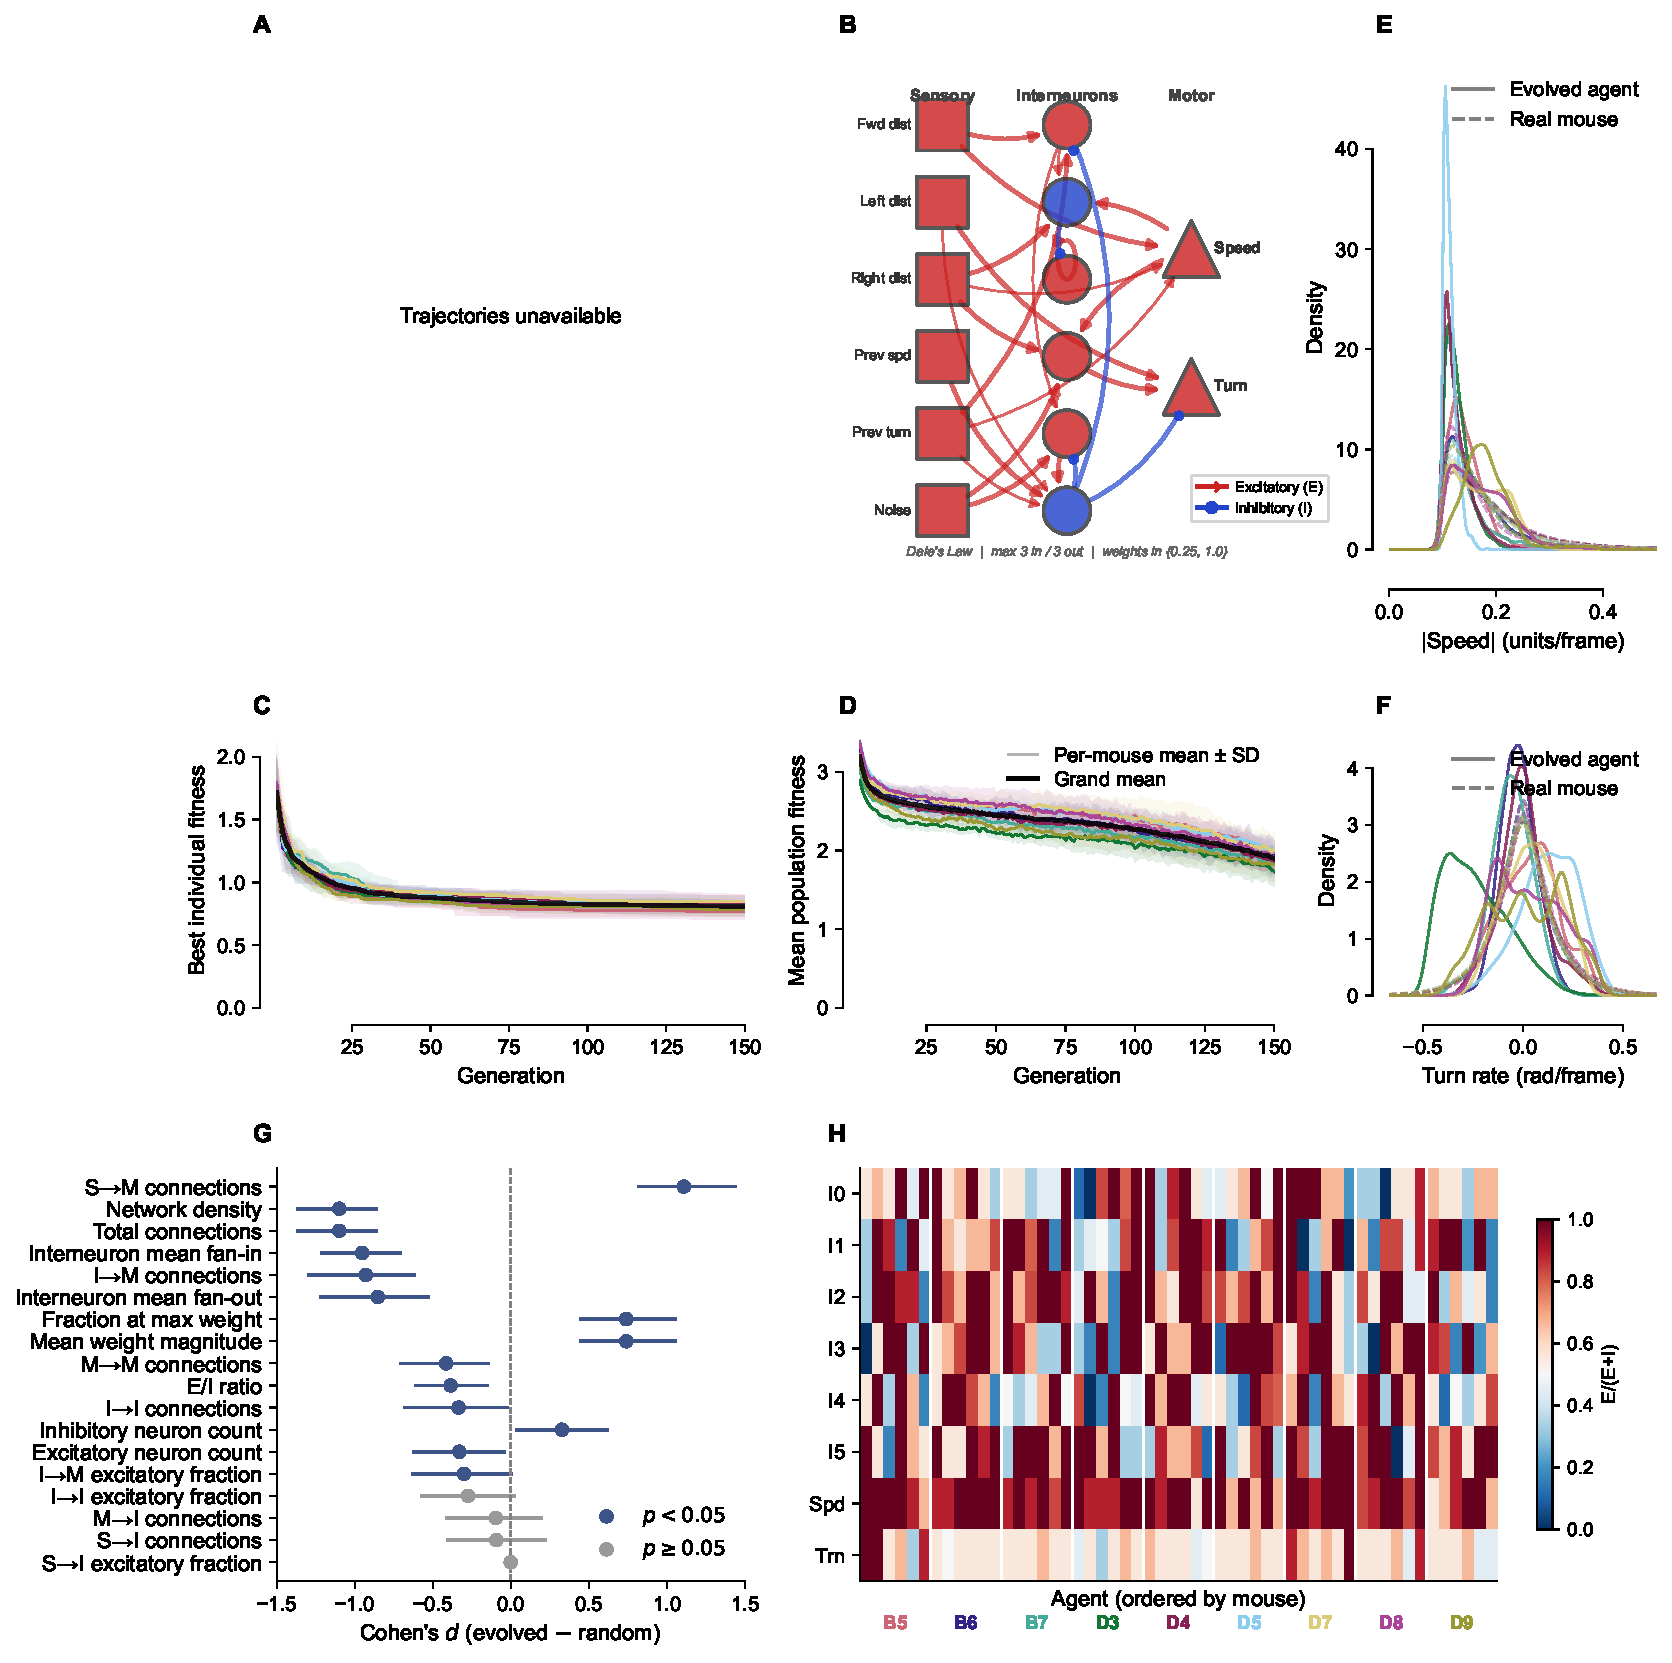
\includegraphics[width=\textwidth]{fig1_system_v2.pdf}
  \caption{\textbf{The constrained neuroevolution system.}
  (A)~Hierarchical binary Y-maze with representative mouse trajectories (5 bouts, B5).
  (B)~14-neuron recurrent agent architecture: 6 sensory inputs (squares), 6 interneurons
  (circles), 2 motor outputs (triangles). Excitatory connections in red, inhibitory in blue.
  Dale's Law, sparse connectivity (max 3 in/3 out), and quantised weights $\{0.25, 1.0\}$
  are enforced throughout evolution.
  (C)~Population mean fitness $\pm$ SD across 6 replicates per mouse over 150 generations
  (lower = better behavioral match). Fitness decreases steeply in generations 1--50, with
  slow improvement continuing to generation 100--120 before plateauing.
  (D)~Best individual fitness per mouse. The best agent in each replicate plateaus earlier
  and more cleanly than the population mean, confirming that evolutionary improvement
  concentrates in the leading individuals.
  (E)~Speed distributions for evolved agents (solid) and real mice (dashed), per mouse.
  Agents reproduce the characteristic speed profile of their target mouse without
  explicit selection for speed.
  (F)~Turn rate distributions for evolved agents (solid) and real mice (dashed), per mouse.
  Agents reproduce the characteristic turn rate profile of their target mouse without
  explicit selection for turn rate statistics.
  (G)~Evolved vs random circuit features: Cohen's $d$ with 95\% bootstrap CI for all
  18 aggregate structural features. Navy $p < 0.05$; grey $p \geq 0.05$. Evolved
  circuits are sparser, more feedforward, and use stronger connections than random agents.
  (H)~E/I balance at generation 150 for all 8 non-sensory neurons ($54 \times 8$
  heatmap, agents ordered by mouse; white lines separate mouse groups). Speed motor (Spd)
  converges uniformly to mean $\approx\statEiBalanceSpeedMean$ excitatory across all mice;
  turn motor (Trn) converges to mean $\approx\statEiBalanceTurnMean$ with greater
  variability, consistent with closed-loop inhibitory modulation of turning.}
  \label{fig:system}
\end{figure}


% ---------------------------------------------------------------------------
\subsection{Architectural constraints impose structural degeneracy,
            yet enable behavioral individuation}
\label{sec:paradox}
% ---------------------------------------------------------------------------
%%% Sources: v1 sec 2.5 (0/18 ANOVA) + 2.6 (9x9 matrix, specialisation index)
%%%          Holdout -> Supplementary
%%% Figure: Fig 2 (Cosine matrix | 18-feature ANOVA summary | 9x9 matrix | spec index bars)
%%% Target: ~700 words
%%% Closing: "Circuits with identical aggregate structure are behaviourally
%%%           specialized. The remainder asks why, and what mechanism
%%%           selection uses to produce it."

Evolved circuits occupy a significantly narrower region of weight space than
randomly initialised constrained agents (pairwise cosine similarity: evolved
$= \statCosineEvolvedRandomEvolvedMean$ vs random
$= \statCosineEvolvedRandomRandomMean$; Mann-Whitney
$p = \statCosineEvolvedRandomMannwhitneyP$;
Supplementary Figure~\ref{fig:supp_cosine_dist}), but the resulting $54 \times 54$
similarity matrix shows no mouse-level block structure
(Figure~\ref{fig:paradox}A). Evolution compresses all circuits toward a
shared structural profile, not toward mouse-specific ones: this is structural
degeneracy at the aggregate level.

Testing 18 aggregate structural features with one-way ANOVA (Benjamini-Hochberg
FDR; \citealt{benjamini1995controlling}) yields
$\statAnovaNSignificantFdr/\statAnovaNFeaturesTested$ significant results.
The smallest raw $p$-value is $\statAnovaTopFeatureP$ (interneuron fan-in);
after BH-FDR correction, all adjusted $p > \statAnovaMinPFdrFloor$
(Figure~\ref{fig:paradox}B). This null result reflects an
architectural floor rather than an evolved property: the same ANOVA, run on an
equal-sized matched sample of randomly initialised (unevolved) constrained agents
(54 agents in a matched 9-group $\times$ 6 design, identical power to the evolved
test), returns an identical 0/18.
The degree limit, quantized weights, and Dale's Law constrain the space of
realisable circuits so tightly that no aggregate structural feature can diverge
across mice regardless of training target. The study is adequately powered to
detect the observed effect sizes: the three largest-effect features each exceed
the 80\% power threshold, and their non-significance reflects the absence of a
detectable effect (Supplementary
Figure~\ref{fig:supp_power}). Both magnitude features likewise show no
between-mouse differences ($p_\text{FDR} = \statAnovaMinPFdrMag$). Every measurable
aggregate structural property converges to a common floor.

Despite this structural uniformity, evolved agents are strongly specialised to
their training mouse. We evaluated each mouse's best agent on all 9 behavioral
targets to construct a $9 \times 9$ cross-mouse generalisation matrix
(Figure~\ref{fig:paradox}D). Within-mouse fitness averaged
$\statCrossMouseDiagMean \pm \statCrossMouseDiagStd$ (diagonal; lower = better
match), compared to
$\statCrossMouseOffMean \pm \statCrossMouseOffStd$ for cross-mouse evaluations
(off-diagonal). The mean behavioral specialisation index
($1 - \text{own/cross fitness}$) was $\statCrossMouseSpecIndex$: cross-mouse
fitness error is $\statCrossMouseSpecGapPct$\% higher than own-mouse error. All
9 mice showed positive indices (\statCrossMouseMostSpecializedMouse{} most
specialised, index $= \statCrossMouseMostSpecializedIndex$;
\statCrossMouseLeastSpecializedMouse{} least, index
$= \statCrossMouseLeastSpecializedIndex$;
Figure~\ref{fig:paradox}C). Specialisation is consistent across all four
fitness components (Supplementary
Figures~\ref{fig:supp_per_metric_heatmaps}--\ref{fig:supp_per_metric_bars})
and within each genetic strain independently of any strain-level grouping
(Supplementary Figures~\ref{fig:supp_strain} and~\ref{fig:supp_weighting_schemes};
Supplementary Table~\ref{tab:supp_weighting}).
Randomly initialised constrained circuits show specialisation indices near zero (mean
$\statRandomNullMeanIndex \pm \statRandomNullStdRatio$; Figure~\ref{fig:paradox}C),
confirming that individual-target optimisation (not the constrained architecture itself)
produces specialisation. Specialisation persists on held-out trajectory data
(Supplementary Analysis~\ref{sec:supp_holdout}).
Specialisation emerges progressively with individual-target training: the population mean
specialisation index rises from $\statSpecEvolSpecInit$ at generation~1 to
$\statSpecEvolSpecFinal$ at generation~150 (Figure~\ref{fig:paradox}E), while
generalist agents trained simultaneously on all nine mice remain near zero throughout
(mean $|\text{bias}|$ at generation~150: $\statSpecEvolGenFinal$). Per-mouse trajectories
are shown in Supplementary Figure~\ref{fig:supp_spec_evol_per_mouse}.

Circuits with identical aggregate structure produce specialised behavior. The
constraint geometry compresses structural variation by design; behavioral
individuation is robust. The remainder of this paper characterises how
this is possible: what degeneracy achieves in this space, and what selection
must do within it.

\begin{figure}[H]
  \centering
  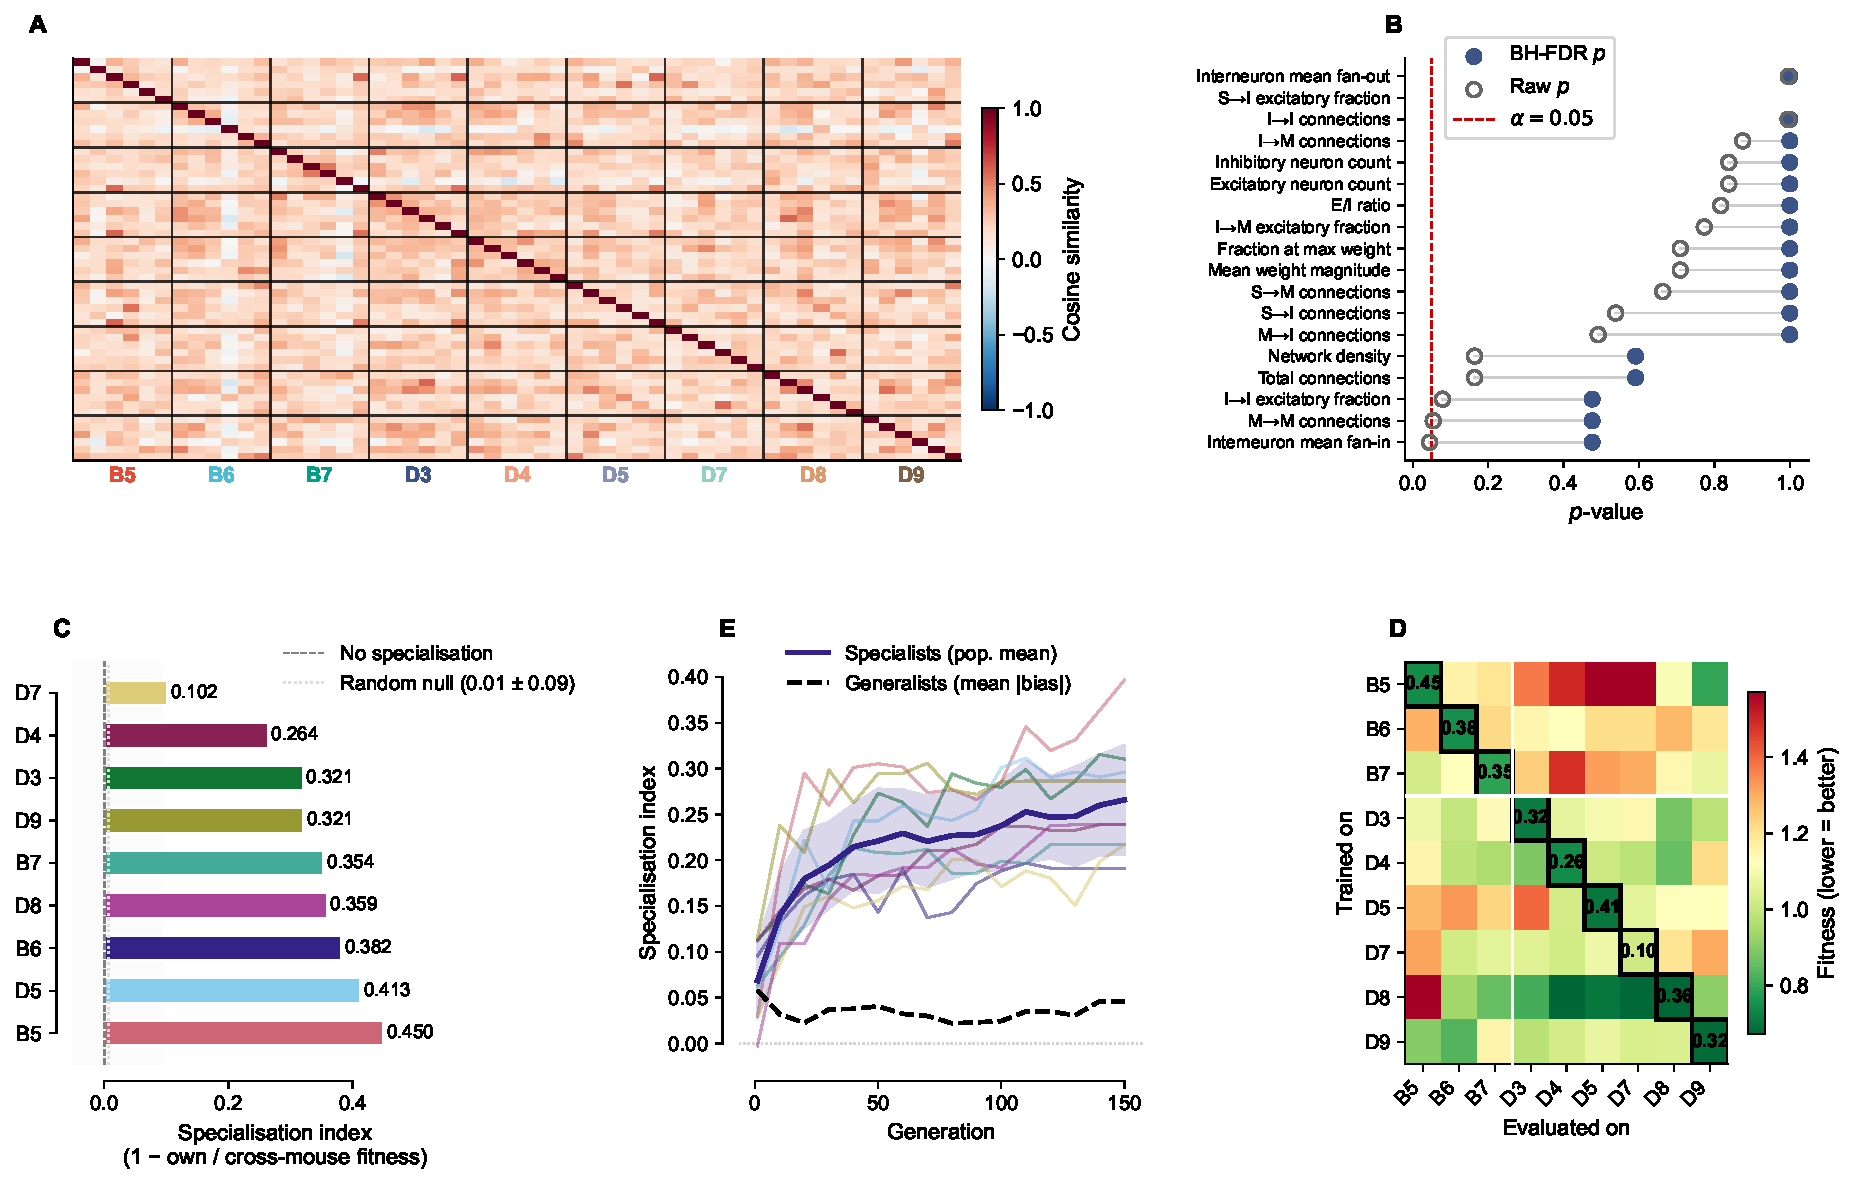
\includegraphics[width=\textwidth]{fig2_paradox_v2.pdf}
  \caption{\textbf{Architectural constraints impose structural degeneracy, yet
  behavioral individuation is robust.}
  (A)~$54 \times 54$ weight cosine similarity heatmap, agents ordered by mouse group
  (separators mark group boundaries). No mouse-level block structure is visible:
  evolution compresses all circuits toward a shared structural region, not toward
  mouse-specific clusters.
  (B)~Raw (open circles) and BH-FDR-corrected (filled, navy) $p$-values for all 18
  aggregate circuit features, sorted ascending by raw $p$, connected by grey lines.
  The smallest raw $p$-value is $\statAnovaTopFeatureP$ (interneuron fan-in); after
  BH-FDR correction, all adjusted $p > \statAnovaMinPFdrFloor$ (red dashed
  line: $\alpha = 0.05$). Zero of 18 features differ across mice regardless of
  correction method.
  (C)~Per-mouse behavioural specialisation index ($1 - \text{own/cross fitness}$),
  sorted descending. All 9 mice show positive indices (dashed line = no specialisation).
  (D)~$9 \times 9$ cross-mouse generalisation matrix. Colour encodes fitness (lower =
  better match), diverging palette centred on the off-diagonal mean. Bold boxes
  highlight diagonal (own-mouse) entries; diagonal annotations show per-mouse
  specialisation index.
  (E)~Specialisation index over 150 generations: coloured per-mouse traces with bold
  population mean (thick line; grey band = $\pm 1$ SD). Dashed black line shows
  generalist mean $|\text{bias}|$, which remains near zero throughout. Specialisation is
  absent at generation 1 and emerges exclusively under individual-target selection pressure.}
  \label{fig:paradox}
\end{figure}



% ---------------------------------------------------------------------------
\subsection{Degeneracy extends to the topology axis: topology variation does
            not predict behavioral identity}
\label{sec:topo_degeneracy}
% ---------------------------------------------------------------------------
%%% Sources: NEW -- A1, A2, A5
%%% Key stats:
%%%   rho_all = \statDegAoneRhoAll (p = \statDegAonePAll)
%%%   rho_within = \statDegAoneRhoWithin, rho_between = \statDegAoneRhoBetween
%%%   A2: rho_topo = \statDegAtwoRhoTopo (p = \statDegAtwoPTopo)
%%%   A5: rho_rand = \statDegAfiveRhoRand (p = \statDegAfivePRand)
%%%   behavioural specialisation confirmed: MW p = \statDegAoneMwBehP
%%% Figure: New Fig A (54x9 heatmap | topo dist vs beh dist scatter |
%%%         rho_rand vs rho_evolved comparison)
%%% Target: ~500 words

The structural floor established in Section~\ref{sec:paradox} operates at the level
of aggregate statistics. Does degeneracy also extend to the specific pattern of
connections? If topology were the axis on which mice differ, we would expect
agents with similar topologies to produce similar behavioral profiles, and agents
trained on the same mouse to converge to more similar topologies than agents
trained on different mice. Neither is the case.

We computed pairwise Spearman correlations between topology distance (Jaccard)
and behavioral profile distance (cosine) across all $\statDegAoneNPairs$ agent
pairs (Figure~\ref{fig:topo_flat}B--C). The overall correlation was
$\rho = \statDegAoneRhoAll$ ($p = \statDegAonePAll$), indistinguishable from
zero. Splitting by pair type makes no difference: within-mouse pairs (agents
trained on the same mouse) give $\rho = \statDegAoneRhoWithin$
($p = \statDegAonePWithin$); between-mouse pairs give
$\rho = \statDegAoneRhoBetween$ ($p = \statDegAonePBetween$). Agents with very
similar topologies are no more behaviorally similar than agents with very
different topologies. Nor did individual-target selection converge topology
within mouse groups: within-mouse Jaccard distances
(mean $= \statDegAoneTopoDistWithinMean$) are indistinguishable from
between-mouse (mean $= \statDegAoneTopoDistBetweenMean$; Mann-Whitney
$p = \statDegAoneMwTopoP$; Figure~\ref{fig:topo_flat}B). The
$9 \times 9$ behavioral specialization structure is robust (Mann-Whitney
$p = \statDegAoneMwBehP$ for within vs between behavioral distance), but it
is invisible in the topology distance matrix.

The same null holds within each mouse. Among the $\statDegAtwoNPairs$
within-mouse replicate pairs, neither topology distance
($\rho = \statDegAtwoRhoTopo$, $p = \statDegAtwoPTopo$) nor magnitude distance
($\rho = \statDegAtwoRhoMag$, $p = \statDegAtwoPMag$) predicts fitness
difference. Partial correlations controlling for the other axis are equally null
(topology controlling for magnitude: $\rho = \statDegAtwoPartialRhoTopo$,
$p = \statDegAtwoPartialPTopo$). The within-mouse fitness landscape is many-to-one
on both structural axes: many topologies achieve equivalent fitness for the same
behavioral target.

Critically, this flatness is not a product of selection. We evaluated 54 randomly
initialised constrained agents (same architecture, no training) on all 9 behavioral
targets and computed the same topology-behavior correlation. Random agents show
$\rho = \statDegAfiveRhoRand$ ($p = \statDegAfivePRand$), and their within/between
behavioral distance structure is absent (Mann-Whitney $p = \statDegAfiveMwWithinP$;
Figure~\ref{fig:topo_flat}C). Degeneracy on the topology axis is thus architectural:
the constraint geometry prevents topology from encoding behavioral identity.

\begin{figure}[H]
  \centering
  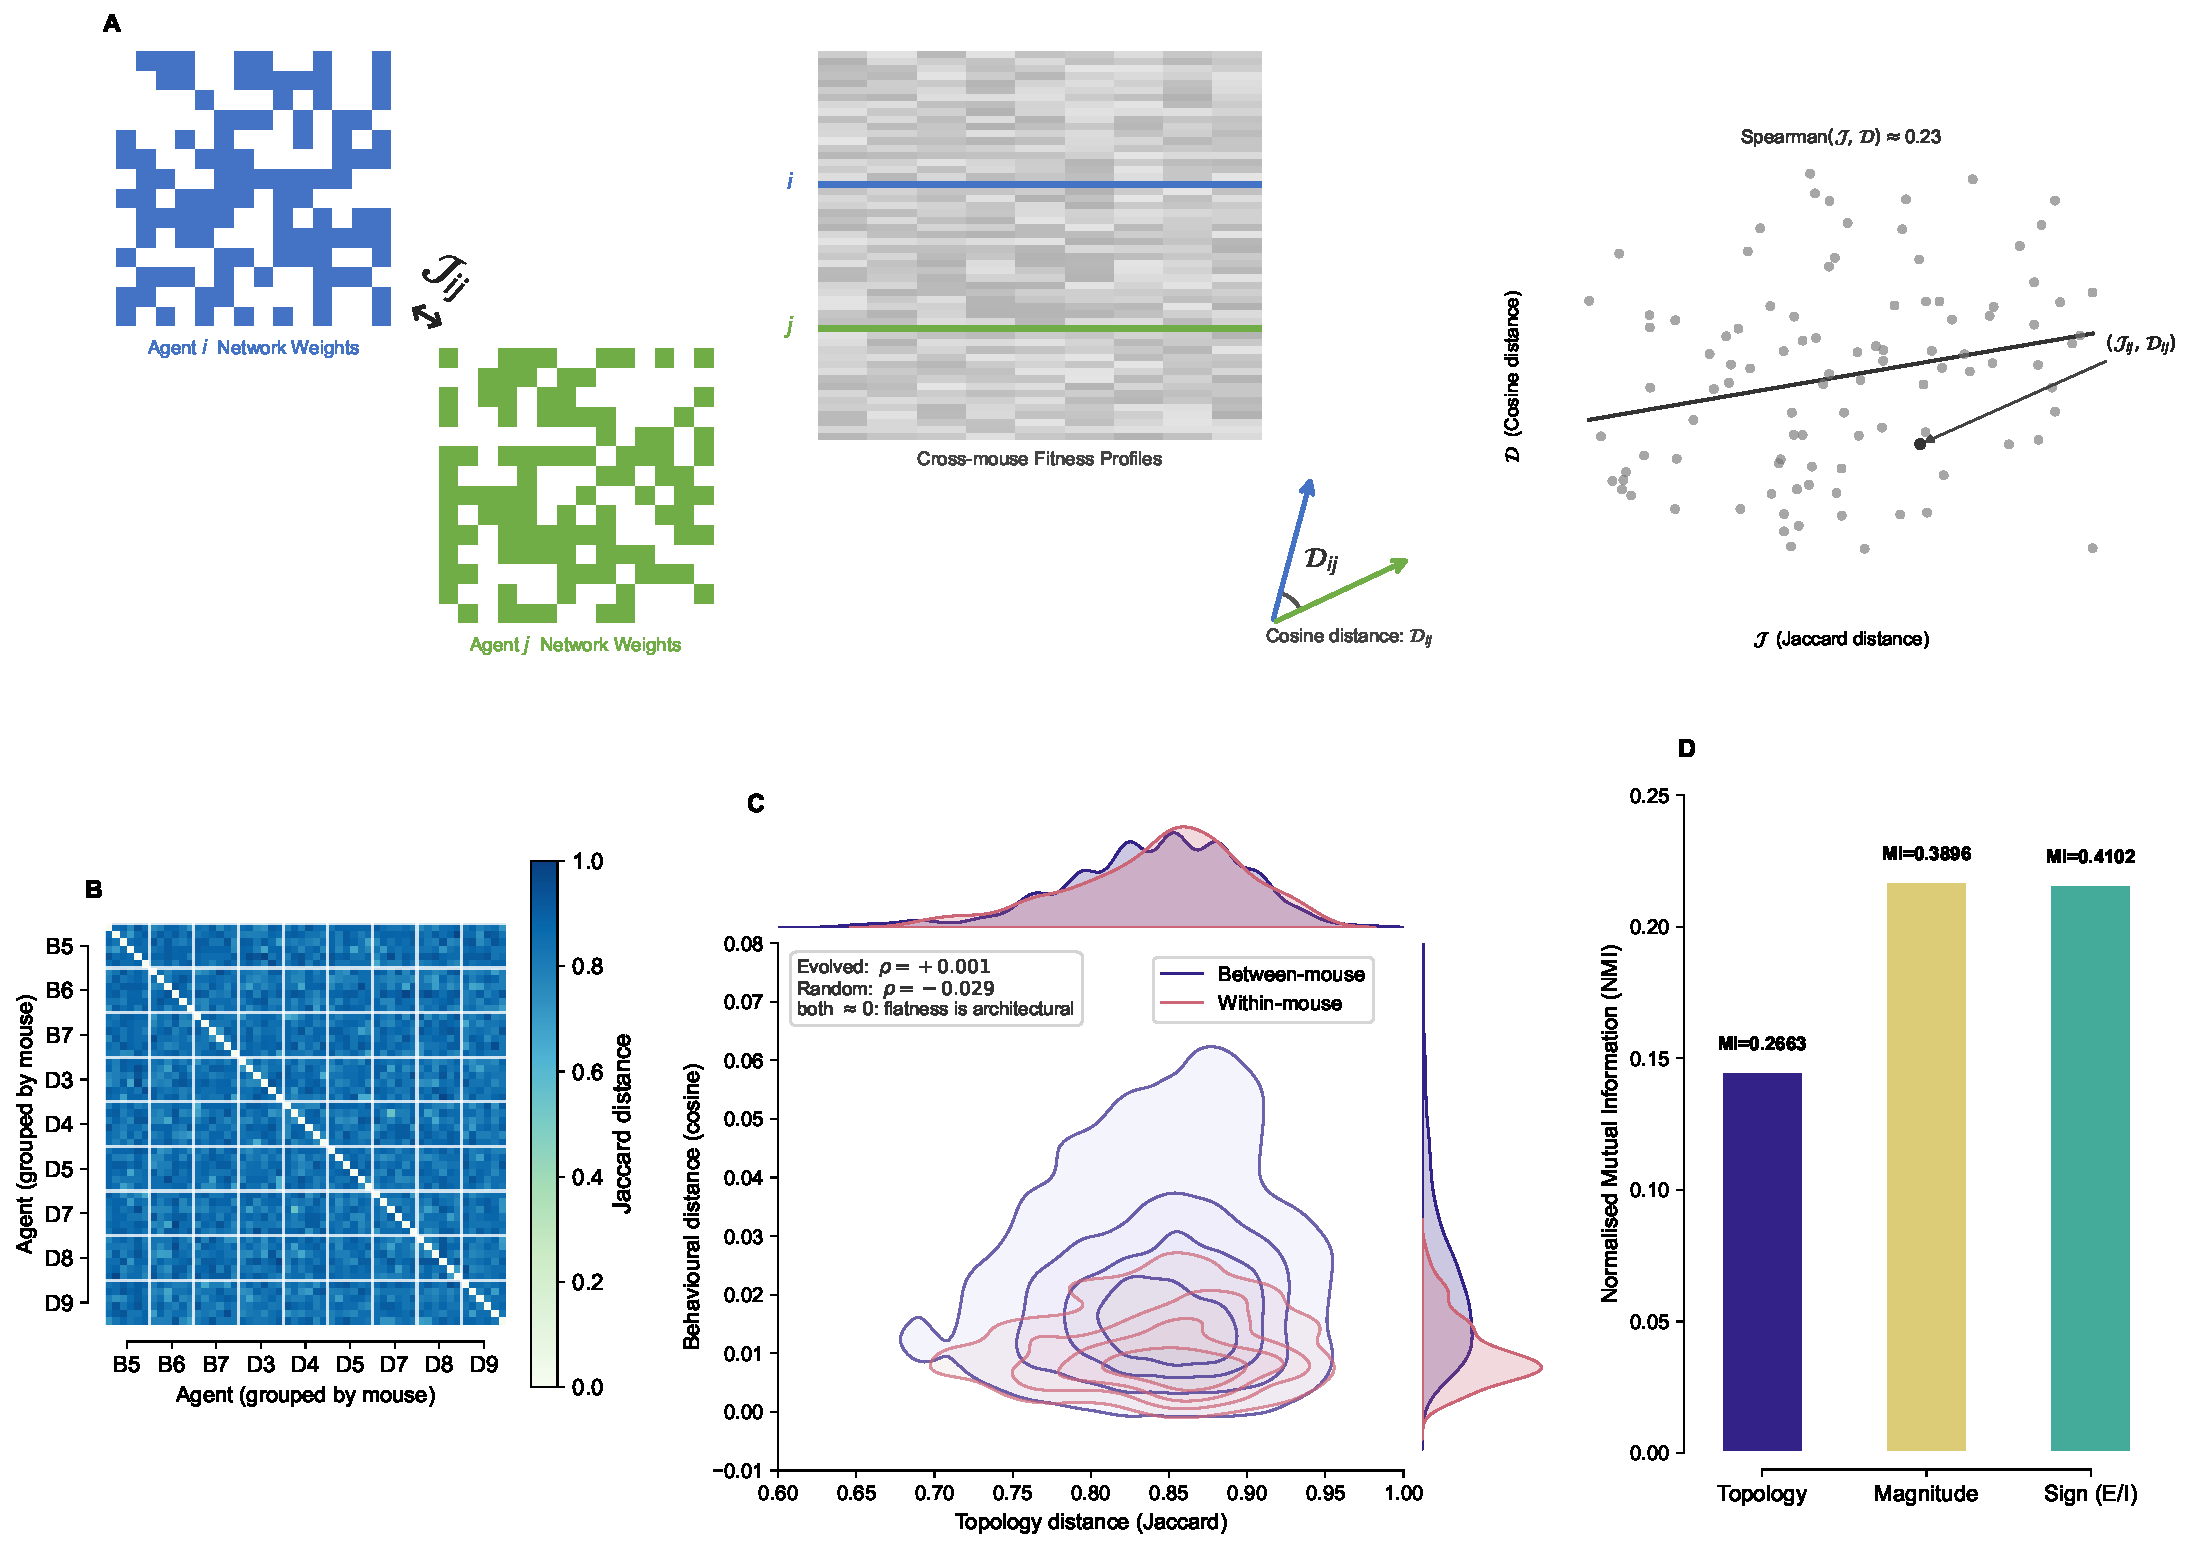
\includegraphics[width=\textwidth]{figA_topo_flat_v2.pdf}
  \caption{\textbf{Structural degeneracy extends across all measurable axes.}
  (A)~Analysis schematic: each agent is characterised by a binary $14 \times 14$
  topology matrix and a 9-dimensional behavioural profile vector; pairwise Jaccard
  distance $J$ (topology) and cosine distance $\mathcal{D}$ (behaviour) are computed
  across all $\statDegAoneNPairs$ agent pairs, and Spearman $\rho$ quantifies their
  correlation.
  (B)~$54 \times 54$ topology Jaccard distance heatmap (agents ordered by mouse
  group; white lines mark boundaries). No within-mouse block structure is visible:
  within-mouse topology distances (mean $= \statDegAoneTopoDistWithinMean$) are
  indistinguishable from between-mouse (mean $= \statDegAoneTopoDistBetweenMean$;
  MW $p = \statDegAoneMwTopoP$). Contrast with the behavioural
  specialisation block structure in Figure~\ref{fig:paradox}A.
  (C)~Joint KDE of topology Jaccard distance vs behavioural cosine distance for all
  $\statDegAoneNPairs$ agent pairs (contours only; rose = within-mouse,
  indigo = between-mouse). Top marginal: topology distance KDE — within- and
  between-mouse distributions overlap completely (MW $p = \statDegAoneMwTopoP$),
  confirming topology flatness. Right marginal: behavioural cosine KDE —
  within-mouse distances are lower than between-mouse (MW $p = \statDegAoneMwBehP$),
  confirming specialisation. Spearman $\rho$ annotated for both evolved
  ($\rho = \statDegAoneRhoAll$, $p = \statDegAonePAll$) and randomly initialised
  constrained agents ($\rho = \statDegAfiveRhoRand$, $p = \statDegAfivePRand$);
  both are indistinguishable from zero: topology-behaviour flatness is architectural.
  (D)~Normalised mutual information (NMI) between each structural axis and mouse
  identity, computed via $k$-means clustering ($k=5$) across all 54 agents.
  Maximum NMI $= \statDegAthreeNmiMax$ across all three axes; all at or below chance
  expectation (adjusted MI near zero or negative across $k = 3$--$9$).
  Reference line at NMI $= 0.5$ provides a calibration anchor for moderate
  association.}
  \label{fig:topo_flat}
\end{figure}


% ---------------------------------------------------------------------------
\subsection{No structural axis carries behavioral identity information}
\label{sec:mi}
% ---------------------------------------------------------------------------
%%% Sources: NEW -- A3
%%% Key stats:
%%%   NMI_topo = \statDegAthreeNmiTopo, NMI_mag = \statDegAthreeNmiMag
%%%   NMI_sign = \statDegAthreeNmiSign, NMI_max = \statDegAthreeNmiMax
%%% Figure: New Fig B (MI/NMI bar chart across three axes)
%%% Target: ~300 words

The correlational analyses of Section~\ref{sec:topo_degeneracy} establish that
topology does not predict behavioral identity. To quantify degeneracy across all
three structural axes (connection topology, synaptic magnitude, and
excitatory/inhibitory sign) simultaneously, we computed mutual information (MI)
between each axis and behavioral identity (the 9-category label indicating which
of the 9 mice each agent was trained on), following the framework of
\citet{tononi1999measures}.

For each structural axis, we represented all 54 agents as feature vectors and
assigned cluster membership via k-means ($k = 5$), grouping agents by structural
similarity on that axis. MI and normalised MI (NMI) were then computed between
cluster assignment and mouse identity (Figure~\ref{fig:topo_flat}D; Methods,
Section~\ref{sec:methods_topo_corr};
Supplementary Figure~\ref{fig:supp_mi_clustering}). No axis carries more than
weak information: NMI $= \statDegAthreeNmiTopo$ for topology,
$\statDegAthreeNmiMag$ for magnitude, and $\statDegAthreeNmiSign$ for
excitatory/inhibitory sign. The maximum NMI across all axes is
$\statDegAthreeNmiMax$, well below NMI $= 0.5$ (moderate association; reference
line, Figure~\ref{fig:topo_flat}D), and at or below chance expectation (adjusted
MI near zero or negative across $k = 3$--$9$; Methods,
Section~\ref{sec:methods_topo_corr}). The system is degenerate on every measurable
structural dimension simultaneously.


% ---------------------------------------------------------------------------
\subsection{Connection topology is causally necessary but structurally
            degenerate; no structural decomposition fingerprints identity}
\label{sec:causal}
% ---------------------------------------------------------------------------
%%% Sources: v1 sec 2.8 (no localisation, 2 sentences) +
%%%          2.9 (dynamics nulls -> Supp Table ref only; permutation 2.39x) +
%%%          2.10 (own-mouse permutation specificity) +
%%%          2.11 (topology vs magnitude -- CORE of this section) +
%%%          A4 (sensitivity RSA null, 1 para, Supp)
%%% Key stats (causal): \statDynamicsPermOverReplicate x MSE,
%%%   topo perm = \statPermutationOptionbRatioTopology x
%%%   mag perm  = \statPermutationOptionbRatioMagnitude x
%%% Key stats (A4, Supp): Mantel rho = \statDegAfourMantelRho
%%%   (p_perm = \statDegAfourMantelPPerm), MW p = \statDegAfourMwP
%%% Figure: Fig 3 (perm MSE topo/mag/baseline | ablation matrix | dose-response)
%%% Target: ~800 words

The analyses above establish that topology variation is uninformative about
behavioral identity. This raises a sharp question: is topology doing anything at
all? The answer is yes: topology is causally necessary, but its role is causal rather
than informational. These are distinct questions with distinct evidential structures.
The permutation analysis is a causal intervention: it asks whether \emph{this} agent's
specific topology is necessary for \emph{its} computation. The correlation analyses of
Sections~\ref{sec:topo_degeneracy}--\ref{sec:mi} are informational: they ask
whether topology variation \emph{across independently evolved agents} encodes
behavioral identity. That topology is causally necessary for each individual
circuit is fully consistent with topology variation being informationally flat
across circuits: any topology drawn from the constrained space provides a
sufficient causal substrate, but no specific topology is uniquely identifying.

\textbf{Topology is causally necessary for computation.}
We performed a source-preserving topology permutation: the specific source-to-target
identity of each connection (which neuron wires to which) was scrambled while every
aggregate structural feature (pathway counts, weight magnitudes, E/I composition) was
preserved exactly. The manipulation therefore isolates specific wiring identity from
the 18 aggregate statistics. Across all 54 agents, permutation
elevated motor output MSE by $\statDynamicsPermOverReplicate\times$ relative to
replicate pairs ($p = \statPermutationOptionbPTopoVsBaseline$, Mann-Whitney;
Figure~\ref{fig:causal}B).
This disruption is mouse-specific: permuted agents lost significantly more
behavioral fitness on their own training mouse than on other mice
($\Delta\text{fit}_\text{own} = \statPermutationOptionaSpecOwnMean$ vs
$\Delta\text{fit}_\text{other} = \statPermutationOptionaSpecOtherMean$; Wilcoxon
signed-rank $p = \statPermutationOptionaWilcoxonP$, unanimous across all 9 mice;
Figure~\ref{fig:causal}A).
A suggestive positive association links the degree of specificity to behavioural
specialisation: the per-mouse specialisation index trends positively with the
own/other $\Delta$fit ratio (Spearman $\rho = \statPermutationOptionaSpearmanRho$,
permutation $p = \statPermutationOptionaSpearmanPermP$, 95\% bootstrap CI
$= [\statPermutationOptionaSpearmanBootCiLo,\, \statPermutationOptionaSpearmanBootCiHi]$,
$n = 9$; Figure~\ref{fig:causal}C). The wide bootstrap interval at $n = 9$ means this
dose-response relationship is indicative rather than firmly established, and does not
bear the weight of the causal conclusion, which rests on the within-agent permutation
effect above.
The specific pattern of connections matters causally for each agent's computation.

\textbf{Topology, not magnitude, is the computational substrate.}
To distinguish the role of connection targets from connection strengths, we
applied a magnitude-only permutation: the $\{0.25, 1.0\}$ strength assignments
were shuffled among each source neuron's existing connections while targets were
held fixed. This produced an MSE ratio of $\statPermutationOptionbRatioMagnitude\times$,
\emph{below} the replicate baseline of $1.0\times$ (Table~\ref{tab:permutation_metrics}).
Shuffling weight strengths makes agents \emph{more} similar in motor output, not
less: with at most 3 connections per source and only two magnitude values,
$\statMagnitudeDegeneracyEvolvedFrac$\% of source neurons carry uniform magnitude
assignments and are unaffected by magnitude shuffling. Synaptic strength is a
degenerate causal axis; connection topology is not.

\begin{table}[H]
  \centering
  \small
  \caption{\textbf{Permutation MSE metrics (normalised to replicate baseline).}
  $p$-values are Mann-Whitney vs replicate pairs.}
  \label{tab:permutation_metrics}
  \begin{tabular}{lcc}
    \toprule
    Condition & MSE ratio & $p$ \\
    \midrule
    Topology permutation  & $\statPermutationOptionbRatioTopology\times$  & $\statPermutationOptionbPTopoVsBaseline$ \\
    Magnitude permutation & $\statPermutationOptionbRatioMagnitude\times$ & $\statPermutationOptionbPMagVsBaseline$  \\
    Between conditions    & \multicolumn{2}{c}{$p = \statPermutationOptionbPTopoVsMag$} \\
    \bottomrule
  \end{tabular}
\end{table}

\textbf{No structural decomposition fingerprints mouse identity.}
If the distributed topology pattern is causally necessary, does any structural
component (local or distributed) carry mouse-specific information? We tested
this at two levels. First, per-source ablation: permuting each neuron's outgoing
connections individually yielded a $54 \times 14$ sensitivity matrix with no
mouse-level organisation: 0 of 14 source neurons significant after Bonferroni
correction, and within-mouse sensitivity profiles no more correlated than
between-mouse profiles ($r_\text{within} = \statSourceSensitivityWithinRMean$,
$r_\text{between} = \statSourceSensitivityBetweenRMean$,
Mann-Whitney $p = \statSourceSensitivityMwP$; Supplementary Figure~\ref{fig:supp_ablation_heatmap}). Second,
even if no single neuron is a fingerprint, the combined \emph{pattern} of
sensitivities across all neurons might be mouse-specific. We tested this with a
representational similarity analysis (RSA): within-mouse agent pairs were no closer
in 14-dimensional sensitivity space than between-mouse pairs (Mann-Whitney
$p = \statDegAfourMwP$), and a Mantel test between the $54 \times 54$ sensitivity
similarity matrix and a mouse-identity matrix found no correlation
(Mantel $\rho = \statDegAfourMantelRho$, permutation $p = \statDegAfourMantelPPerm$;
Supplementary Figure~\ref{fig:supp_sensitivity_rsa}).

Connection topology is causally necessary for computation and is individually
calibrated to each mouse's behavioral target. But the specific topology an agent
uses is degenerate with respect to behavioral identity: agents with very different
topologies can achieve the same behavioral fitness, and no structural decomposition
(individual neurons or the distributed pattern of ablation sensitivities)
identifies a mouse from its circuit. What individual-target selection achieves
within this degenerate structural space is the question the following section
addresses.

\begin{figure}[H]
  \centering
  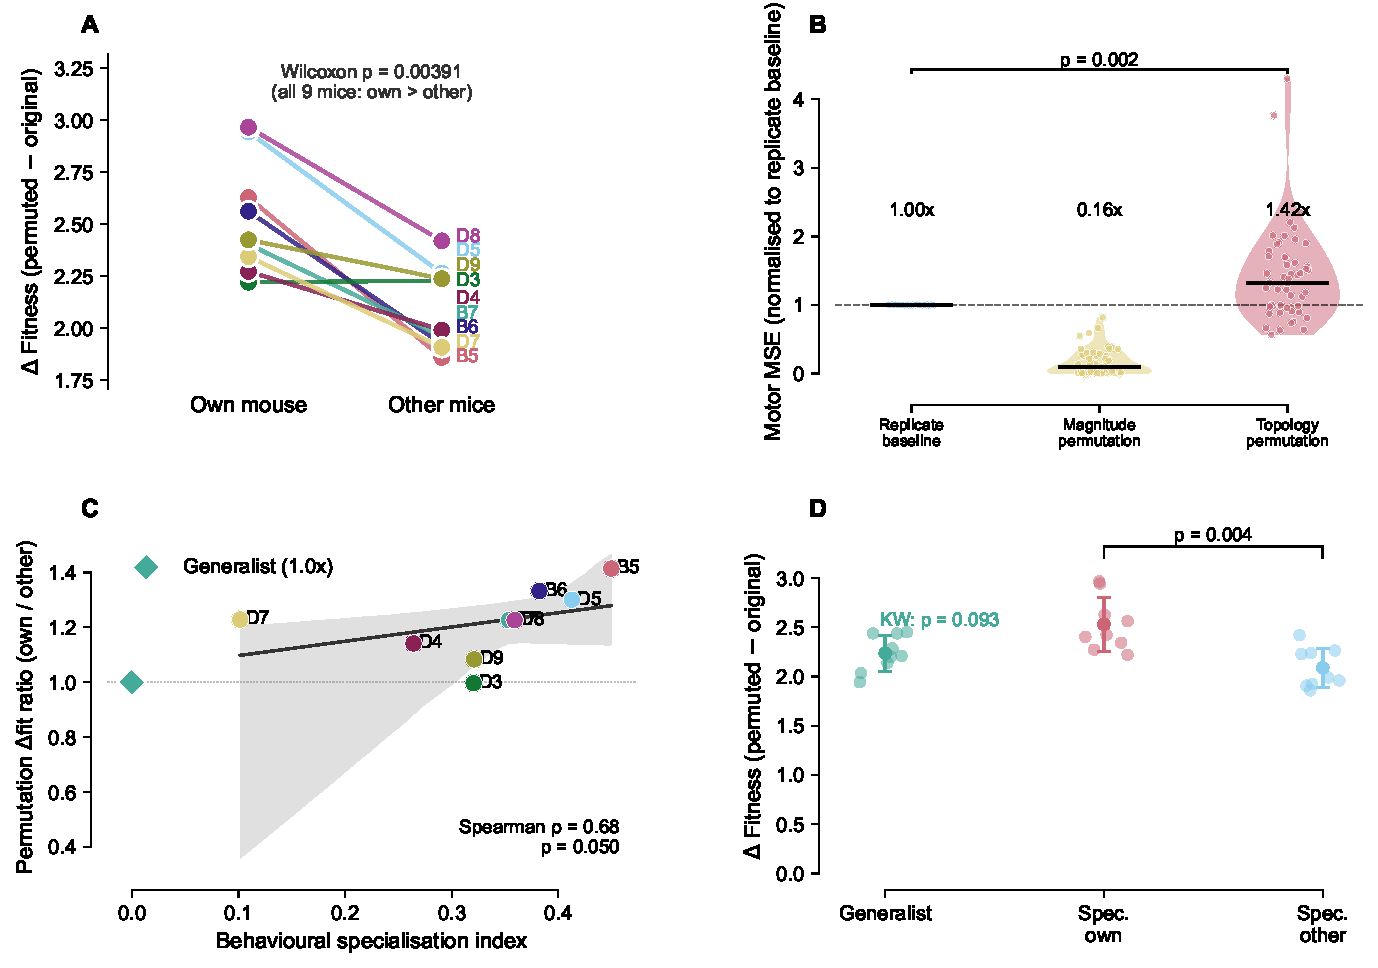
\includegraphics[width=\textwidth]{fig3_causal_v2.pdf}
  \caption{\textbf{Topology is causally necessary but structurally degenerate.}
  (A)~Slope graph: permutation $\Delta$fit on own mouse vs other mice for each
  of the 9 specialist mice (coloured lines). All 9 lines slope upward; own-mouse
  degradation is unanimously greater (Wilcoxon $p = \statPermutationOptionaWilcoxonP$).
  (B)~Motor MSE under topology permutation, magnitude permutation, and replicate
  baseline. Violin + strip plots; median marked. Topology permutation elevates MSE
  ($\statPermutationOptionbRatioTopology\times$ baseline); magnitude permutation
  reduces it ($\statPermutationOptionbRatioMagnitude\times$), reflecting
  architectural degeneracy in weight strengths.
  (C)~Dose-response: per-mouse behavioural specialisation index vs permutation
  $\Delta$fit ratio (own/other). More specialised mice show greater permutation
  specificity (Spearman $\rho = \statPermutationOptionaSpearmanRho$, permutation
  $p = \statPermutationOptionaSpearmanPermP$, 95\% bootstrap CI
  $= [\statPermutationOptionaSpearmanBootCiLo,\, \statPermutationOptionaSpearmanBootCiHi]$,
  $n = 9$). The generalist (teal diamond) anchors ratio $= 1.00\times$.
  (D)~Generalist control: permutation $\Delta$fit for generalist agents,
  specialist-own, and specialist-other conditions (mean $\pm$ SD, individual
  points overlaid). Generalists show no own-mouse elevation
  (Kruskal-Wallis $p = \statGeneralistKruskalP$, n.s.); specialists show
  unanimous own $>$ other (Wilcoxon $p = \statPhaseThreebWilcoxonP$).
  Per-source ablation (54~agents $\times$ 14 source neurons) is shown in
  Supplementary Figure~\ref{fig:supp_ablation_heatmap}.}
  \label{fig:causal}
\end{figure}



% ---------------------------------------------------------------------------
\subsection{Selection shapes functional sensitivity commitment;
            individual-target training is necessary}
\label{sec:sensitivity}
% ---------------------------------------------------------------------------
%%% Sources: v1 sec 2.12 (generalist) + A6
%%% Key stats:
%%%   topo MW p = \statDegAsixMwTopoP (gen = \statDegAsixGenTopoMean,
%%%                                    spec = \statDegAsixSpecTopoMean)
%%%   mean fitness cost = \statDegAsixMeanCostPct\%
%%%   spec sens var = \statDegAsixSpecSensVarMean,
%%%   gen sens var  = \statDegAsixGenSensVarMean
%%%   ratio = \statDegAsixVarRatio x
%%% Figure: New Fig C (topo similarity gen vs spec | fitness cost per mouse |
%%%         sensitivity variance per neuron spec vs gen)
%%% Target: ~600 words

Having established that degeneracy operates on every structural axis, we ask
what individual-target selection actually achieves. We trained six generalist agents
simultaneously on all 9 mice, using fitness equal to the mean across all 9 behavioral
targets, with the same architecture, constraints, and evolutionary parameters as the
per-mouse runs.

\textbf{Generalists and specialists share statistically indistinguishable topological diversity.}
Generalist agents converged structurally, as expected from the architectural floor
(Section~\ref{sec:paradox}). Pairwise topology cosine similarity was
$\statDegAsixGenTopoMean$ for generalists and $\statDegAsixSpecTopoMean$ for
specialists (Mann-Whitney $p = \statDegAsixMwTopoP$;
Figure~\ref{fig:sensitivity_commitment}A). Individual-target training does not
produce a more committed or distinctive topology. The axis on which selection
acts is not topological.

\textbf{Individual-target training shapes functional sensitivity commitment.}
What it does produce is a committed functional sensitivity structure. We measured
sensitivity variance per neuron (the variance of each neuron's ablation
sensitivity across replicates) as a readout of how consistently a circuit
commits to particular pathways. Specialist agents show high, varied sensitivity
($\bar{\sigma}^2 = \statDegAsixSpecSensVarMean$ per neuron): individual-target
training produces circuits that are each strongly committed to perturbations of
specific pathways, but which pathways vary across replicates, even within the
same mouse. Consistent with the RSA null above
(Supplementary Figure~\ref{fig:supp_sensitivity_rsa}), within-mouse sensitivity
profiles are no more similar to each other than to profiles from a different mouse:
at generation~150 the pairwise cosine similarity is if anything marginally lower
within-mouse ($\statClaimTwentyEightWithinSim$) than between-mouse
($\statClaimTwentyEightBetweenSim$), but this small gap does not survive a
pseudoreplication-aware test (label-permutation $p = \statClaimTwentyEightPermP$;
the naive Mann-Whitney $p = \statClaimTwentyEightMwP$ treats the
non-independent agent-pairs as independent and is anticonservative). We therefore do
not claim that replicates commit to \emph{distinct} pathways; the defensible reading is
that no shared, mouse-specific pathway signature emerges. Selection builds the strength
of functional commitment, not convergence to specific pathways. Generalist agents show substantially lower sensitivity variance
($\bar{\sigma}^2 = \statDegAsixGenSensVarMean$; ratio
$= \statDegAsixVarRatio\times$; per-neuron Mann-Whitney $p = \statDegAsixVarMwP$,
one-sided, $n = 14$ neurons per group; Figure~\ref{fig:sensitivity_commitment}C),
reflecting weaker, more distributed sensitivity to perturbations across all pathways.
Generalists achieve comparable structural diversity at the cost of functional
specialization of any kind.

\textbf{Individual targets are necessary: the fitness cost of generalism.}
Generalist behavioral fitness was $\statDegAsixMeanCostPct$\% worse than
specialist fitness on average across mice (range
$\statDegAsixMinCostPct$--$\statDegAsixMaxCostPct$\%;
Figure~\ref{fig:sensitivity_commitment}B). The hardest mouse to generalise across
was \statDegAsixHardestMouse{} ($\statDegAsixMaxCostPct$\% cost) and the easiest
was \statDegAsixEasiestMouse{} ($\statDegAsixMinCostPct$\% cost). The generalist's
permutation profile confirms the mechanism: it shows no own-mouse elevation in
permutation $\Delta$fit (Kruskal-Wallis $p = \statGeneralistKruskalP$), in contrast
to specialists where own-mouse degradation is unanimous
(Figure~\ref{fig:causal}D). A generalist circuit is
disrupted like a specialist evaluated on its wrong mouse: partially calibrated to
everyone, fully calibrated to none.

The fitness cost confirms that generalists do not simply fail to converge: relative
to the per-mouse specialist fitness (mean of replicates), generalist error is higher
by $\statDegAsixCostRatioOfMeans$\% on a ratio-of-means basis (per-mouse range
$\statDegAsixMinCostPct$--$\statDegAsixMaxCostPct$\%), yet they still reproduce each
mouse's behaviour well above chance, confirming clear behavioral learning. The low
sensitivity variance is therefore not underfitting: it reflects the fact that
generalist replicates, each having learned a working solution, show weaker and
more distributed sensitivity to pathway perturbations, with no strong commitment
to any particular subset of pathways.

The A4 sensitivity RSA result (Supplementary Figure~\ref{fig:supp_sensitivity_rsa})
and the A6 sensitivity variance result are compatible and jointly clarify the
mechanism. The \emph{geometry} of the sensitivity profile does not fingerprint mouse
identity (A4: which neurons an agent is sensitive to is not individually consistent).
What individuates a specialist is the \emph{strength} of its sensitivity commitment:
how strongly, and how variably across replicates, its circuits commit to specific
pathway perturbations, even as the particular pathways committed to differ freely.
Individual-target training builds this commitment; generalist training cannot
(Figure~\ref{fig:sensitivity_commitment}D). This commitment co-develops with
behavioural specialisation throughout training: sensitivity variance in specialist
circuits remains elevated above the generalist level from approximately generation~20
onward, while within-mouse sensitivity profiles diverge from a shared baseline as
circuits become mouse-committed (Supplementary Figure~\ref{fig:supp_sens_commitment_evo}).

What individual-target selection shapes is therefore not a distinctive topology, but
the \emph{strength} of a circuit's functional sensitivity commitment: specialists develop
higher sensitivity variance across replicates than generalists, while the RSA null
(Supplementary Figure~\ref{fig:supp_sensitivity_rsa}) shows that the specific committed
pathways are not individually consistent. Behavioral individuation in this constrained
system is thus expressed as a magnitude of functional commitment, not as a distinctive
circuit structure or a mouse-specific pathway signature.

\begin{figure}[H]
  \centering
  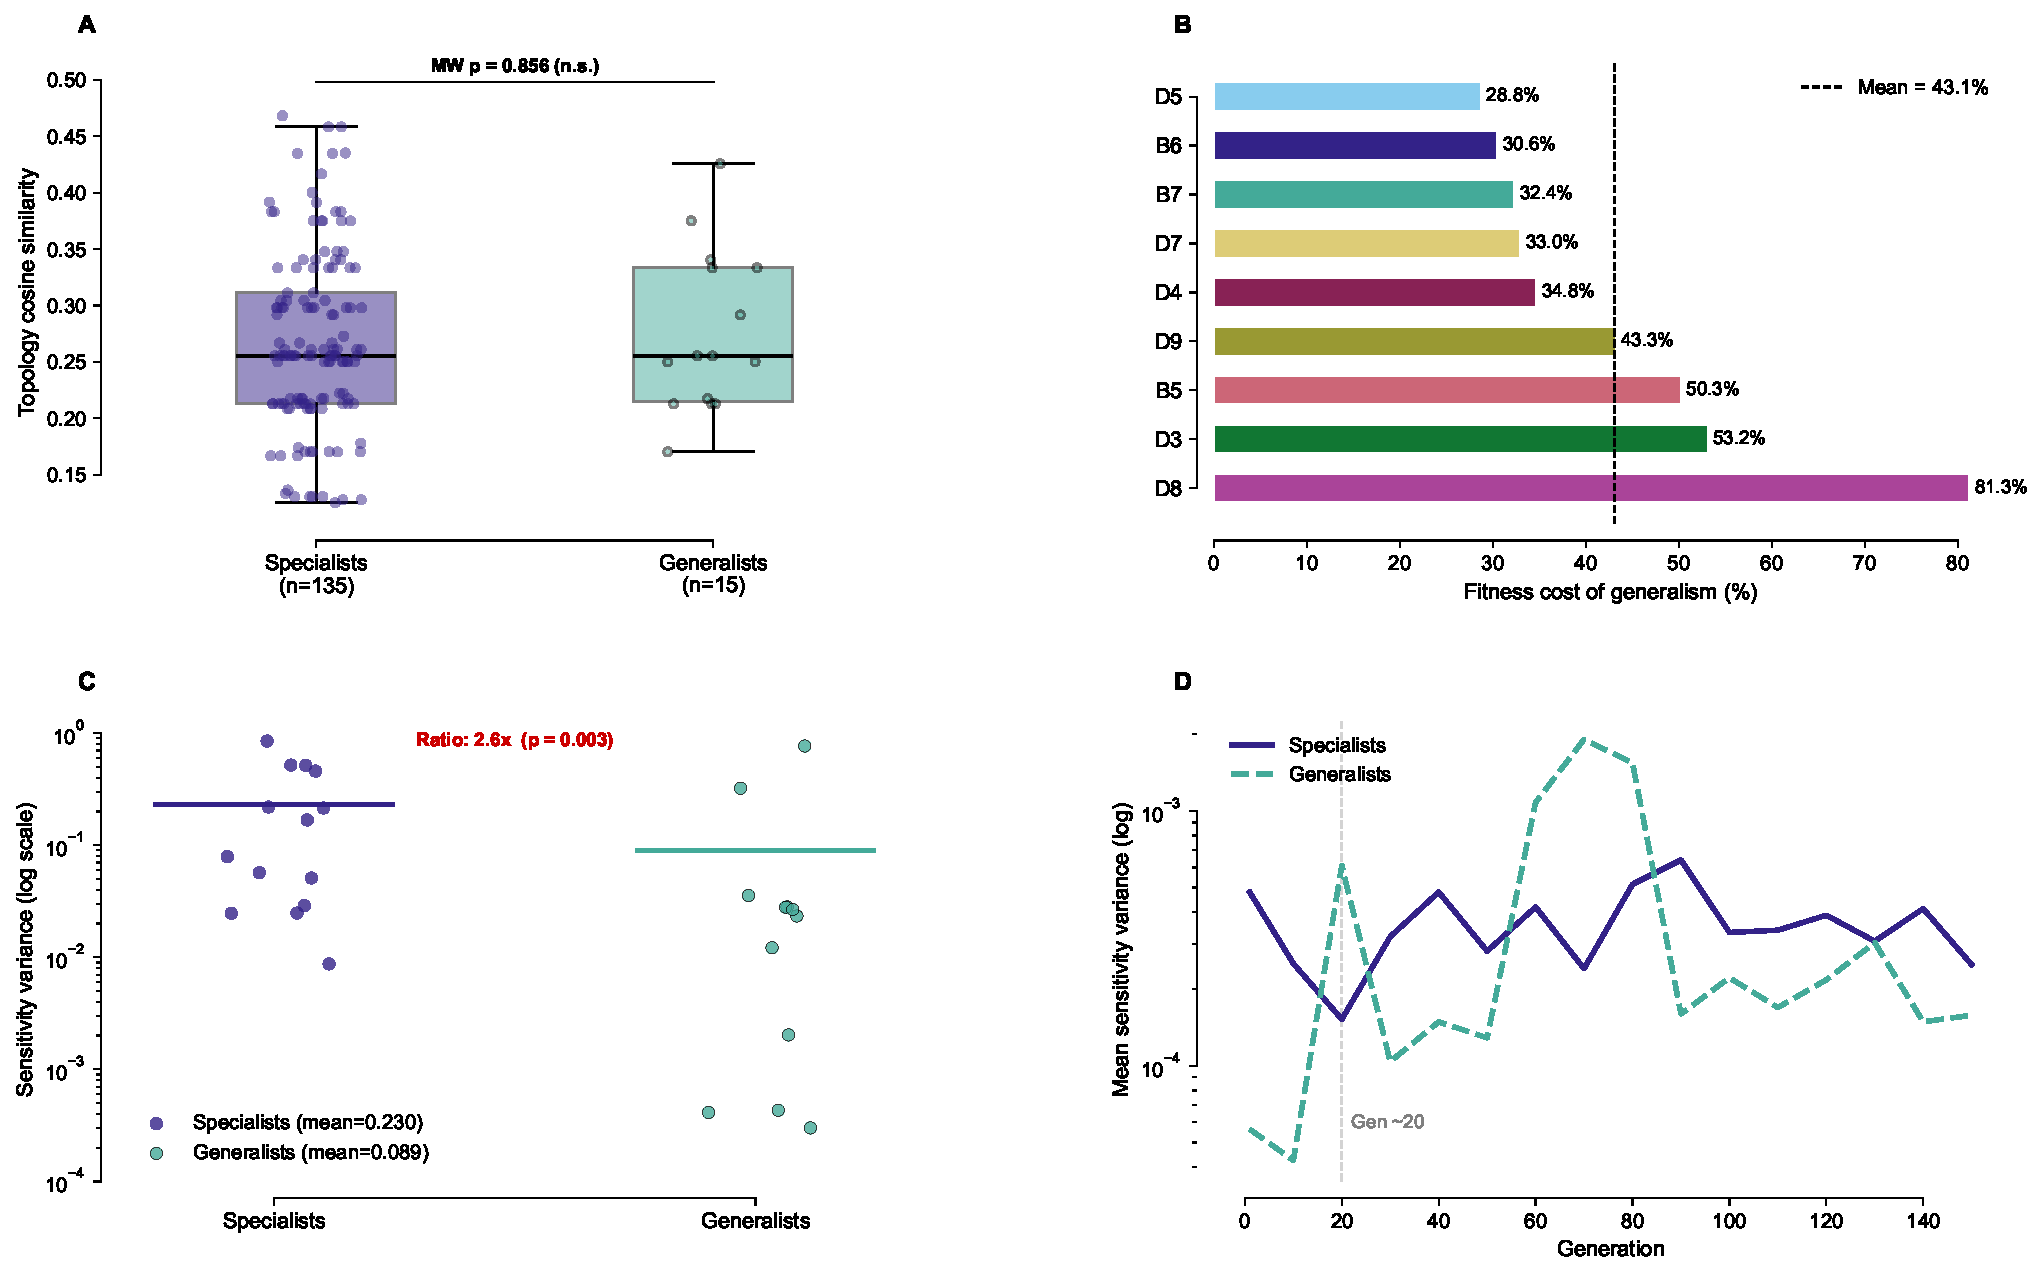
\includegraphics[width=\textwidth]{figC_sensitivity_v2.pdf}
  \caption{\textbf{Selection shapes functional sensitivity commitment.}
  (A)~Topology cosine similarity for generalist and specialist agents (box + strip,
  Mann-Whitney $p = \statDegAsixMwTopoP$). Generalists and specialists show
  indistinguishable topological diversity, confirming that individual-target
  training does not act on topology.
  (B)~Fitness cost of generalism per mouse (percentage worse than specialist fitness),
  sorted descending. Dashed line = mean ($\statDegAsixMeanCostPct$\%).
  (C)~Sensitivity variance per neuron for specialists vs generalists (log scale;
  individual neuron points shown, $n = 14$ per group). Specialists show high, varied
  sensitivity ($\bar{\sigma}^2 = \statDegAsixSpecSensVarMean$); generalists show
  substantially lower sensitivity variance ($\bar{\sigma}^2 = \statDegAsixGenSensVarMean$).
  The specialist:generalist variance ratio is $\statDegAsixVarRatioWithin$--$\statDegAsixVarRatio\times$
  (within-mouse-pooled to across-all-54 definitions; hierarchical-bootstrap 95\% CI
  $[\statDegAsixVarBootCiLo,\,\statDegAsixVarBootCiHi]$). At the mouse level (the independent
  unit), $\statDegAsixMouseNPos$/9 mice exceed the generalist (one-sample Wilcoxon
  $p = \statDegAsixMouseWilcoxP$); the per-neuron Mann-Whitney is $p = \statDegAsixVarMwP$
  (one-sided).
  (D)~Mean sensitivity variance over 150 generations: specialists (solid, blue) vs
  generalists (dashed, orange), log scale. The endpoint shown in Panel~C is the product
  of a progressive process: specialist sensitivity variance diverges from the generalist
  level from approximately generation~20 onward, and continues to rise throughout
  training. Individual-target selection specifically builds functional commitment;
  generalist training does not.}
  \label{fig:sensitivity_commitment}
\end{figure}


% ---------------------------------------------------------------------------
\subsection{Representational geometry is also degenerate}
\label{sec:rep_geometry}
% ---------------------------------------------------------------------------

The structural, causal, and functional analyses above establish degeneracy across
multiple levels of circuit description. Does this degeneracy extend to the
representational level (to the geometry of neuronal activity embeddings)?
A theoretical framework by \citet{pezon2026gerstner} makes this question precise:
even when different circuits produce identical latent dynamics, circuit structure may
leave a ``footprint'' in neuronal embedding geometry, defined as the row loadings of
the activity matrix under principal components analysis (PCA). The framework holds
that circuit structure constrains the distribution of single-neuron functional
properties even when the low-dimensional dynamics are equivalent across circuits.
We operationalise this as a concrete, testable prediction about embedding geometry:
if circuit structure leaves such a footprint, circuits with distinct architectures
should differ in the intrinsic dimensionality or connected-component structure of
their neuronal embeddings, even when their behaviorally relevant dynamics are
identical.

We tested this prediction directly. For each of the 54 best-evolved agents (one per
mouse per replicate), we re-simulated navigation across 20 bouts of up to 2000 frames
each and recorded the full 14-dimensional neural state at every timestep. PCA was
applied to the resulting $(N_\text{neurons} \times T_\text{total})$ activity matrix
for each agent, retaining the top 6 components (which explained \textgreater 90\% of
variance in most agents; Supplementary Figure~\ref{fig:supp_act_emb_ctrl}), yielding neuronal embedding
coordinates of shape $14 \times 6$. Before testing the main question, we verified that
these embeddings are informative at the small scale of our system ($N = 14$): the two
motor neurons (speed, neuron~12; turn, neuron~13) were consistently more separated
from each other in PC1--PC2 loading space than the typical interneuron pair
($\statActEmbMotorDist \pm \statActEmbMotorDistStd$ versus
$\statActEmbInterDist \pm \statActEmbInterDistStd$; Mann-Whitney $p < 0.001$;
Supplementary Figure~\ref{fig:supp_act_emb_ctrl}). Note that PC loading orientation
varies across agents due to the sign ambiguity of independent PCA solutions; all
pairwise comparisons use Procrustes alignment to remove this ambiguity.

The manifold dimensionality of these circuits was near-maximal: the effective
dimensionality at the 90\% variance threshold was
$\statActEmbEffDim \pm \statActEmbEffDimStd$ out of a maximum of 6 retained components,
and the participation ratio was $\statActEmbPR \pm \statActEmbPRStd$, with no
mouse-specific pattern (Supplementary Figure~\ref{fig:supp_b3_dim}). Individual-target circuits
do not converge on a low-dimensional representational cluster; they explore almost
the full embedding space available to them.

To test whether individual-target selection produces convergence in activity embedding
space, we computed pairwise Procrustes distances between the PC loading matrices of all
$54 \times 53 / 2 = 1{,}431$ agent pairs, using orthogonal Procrustes alignment to
remove the sign and rotation ambiguity introduced by independent PCA solutions.
Within-mouse pairs ($n = 135$; 15 pairs per mouse across 6 replicates) showed Procrustes
distances of $\statActEmbWithinProc \pm \statActEmbWithinProcStd$, statistically
indistinguishable from between-mouse pairs ($n = 1{,}296$;
$\statActEmbBetweenProc \pm \statActEmbBetweenProcStd$; Mann-Whitney
$p = \statActEmbRsaMwP$; Figure~\ref{fig:embedding_rsa}A). This null result was robust
across six independent similarity metrics spanning three activity-matrix construction
modes (Procrustes; $p = \statActEmbRobustPLo$--$\statActEmbRobustPHi$),
representational dissimilarity analysis ($p = \statActEmbRsaMwPVal$),
centred kernel alignment ($p = \statActEmbCkaMwPVal$), and covariance Frobenius
distance ($p = \statActEmbCovFrobMwPVal$; Supplementary Figure~\ref{fig:supp_emb_robustness}). Generalist agents,
which were not trained on any individual mouse, occupied the same region of embedding
space as specialists ($\statActEmbGenProc \pm \statActEmbGenProcStd$; Mann-Whitney
versus specialist within-mouse pairs, $p = \statActEmbGenVsWithinP$;
Figure~\ref{fig:embedding_rsa}A).

Degeneracy in this system therefore extends to the representational level: the circuit
variation produced by individual-target selection is insufficient to leave a detectable
footprint in neuronal embedding geometry. Within the framework of
\citet{pezon2026gerstner}, the circuit structure imposes no detectable constraint on
the topology of the similarity-space point cloud (whether measured by Procrustes
distance or effective dimensionality). The footprint is absent.

To test whether this representational degeneracy is simply a downstream consequence of
the structural and functional degeneracy already established, we ran three dissociation
tests using permutation Mantel tests on the full $1{,}431$-pair upper triangle of the
Procrustes distance matrix. Representational distance was uncorrelated with behavioral
distance (Mantel $\rho = \statActEmbBehMantelRho$, $p = \statActEmbBehMantelP$) and with functional
sensitivity distance (Mantel $\rho = \statActEmbSensMantelRho$, $p = \statActEmbSensMantelP$),
confirming that activity geometry is uncorrelated with the functional axis that
individual-target selection does shape. Representational distance showed a weak but significant
positive correlation with topological distance (Mantel $\rho = \statActEmbTopoMantelRho$,
$p < 0.001$; Figure~\ref{fig:embedding_rsa}B, E, H): circuits sharing more topological
scaffold tend toward slightly more similar representations, as expected if structure
constrains dynamics to some degree. This residual structure$\to$representation coupling
does not, however, translate into mouse identity: within-mouse representations are no
closer than between-mouse (MW $p = \statActEmbRsaMwP$), and topology itself carries
negligible identity information (NMI $= \statDegAthreeNmiTopo$;
Section~\ref{sec:mi}). Representational geometry is therefore degenerate with respect to
behavioral identity, even though it is weakly constrained by circuit structure.

Individual-target selection shapes \emph{what} each circuit computes (as shown by
the behavioural specialisation and functional sensitivity results) but not \emph{how}
that computation is organised in representational space. The geometry of neural
activity, like the topology of circuit wiring, is invisible to individual-target
selection. Whether this independence extends to the dynamical geometry of the circuit
(its stability regime, attractor landscape, and driven trajectory structure) is
examined in the following section.

\begin{figure}[H]
  \centering
  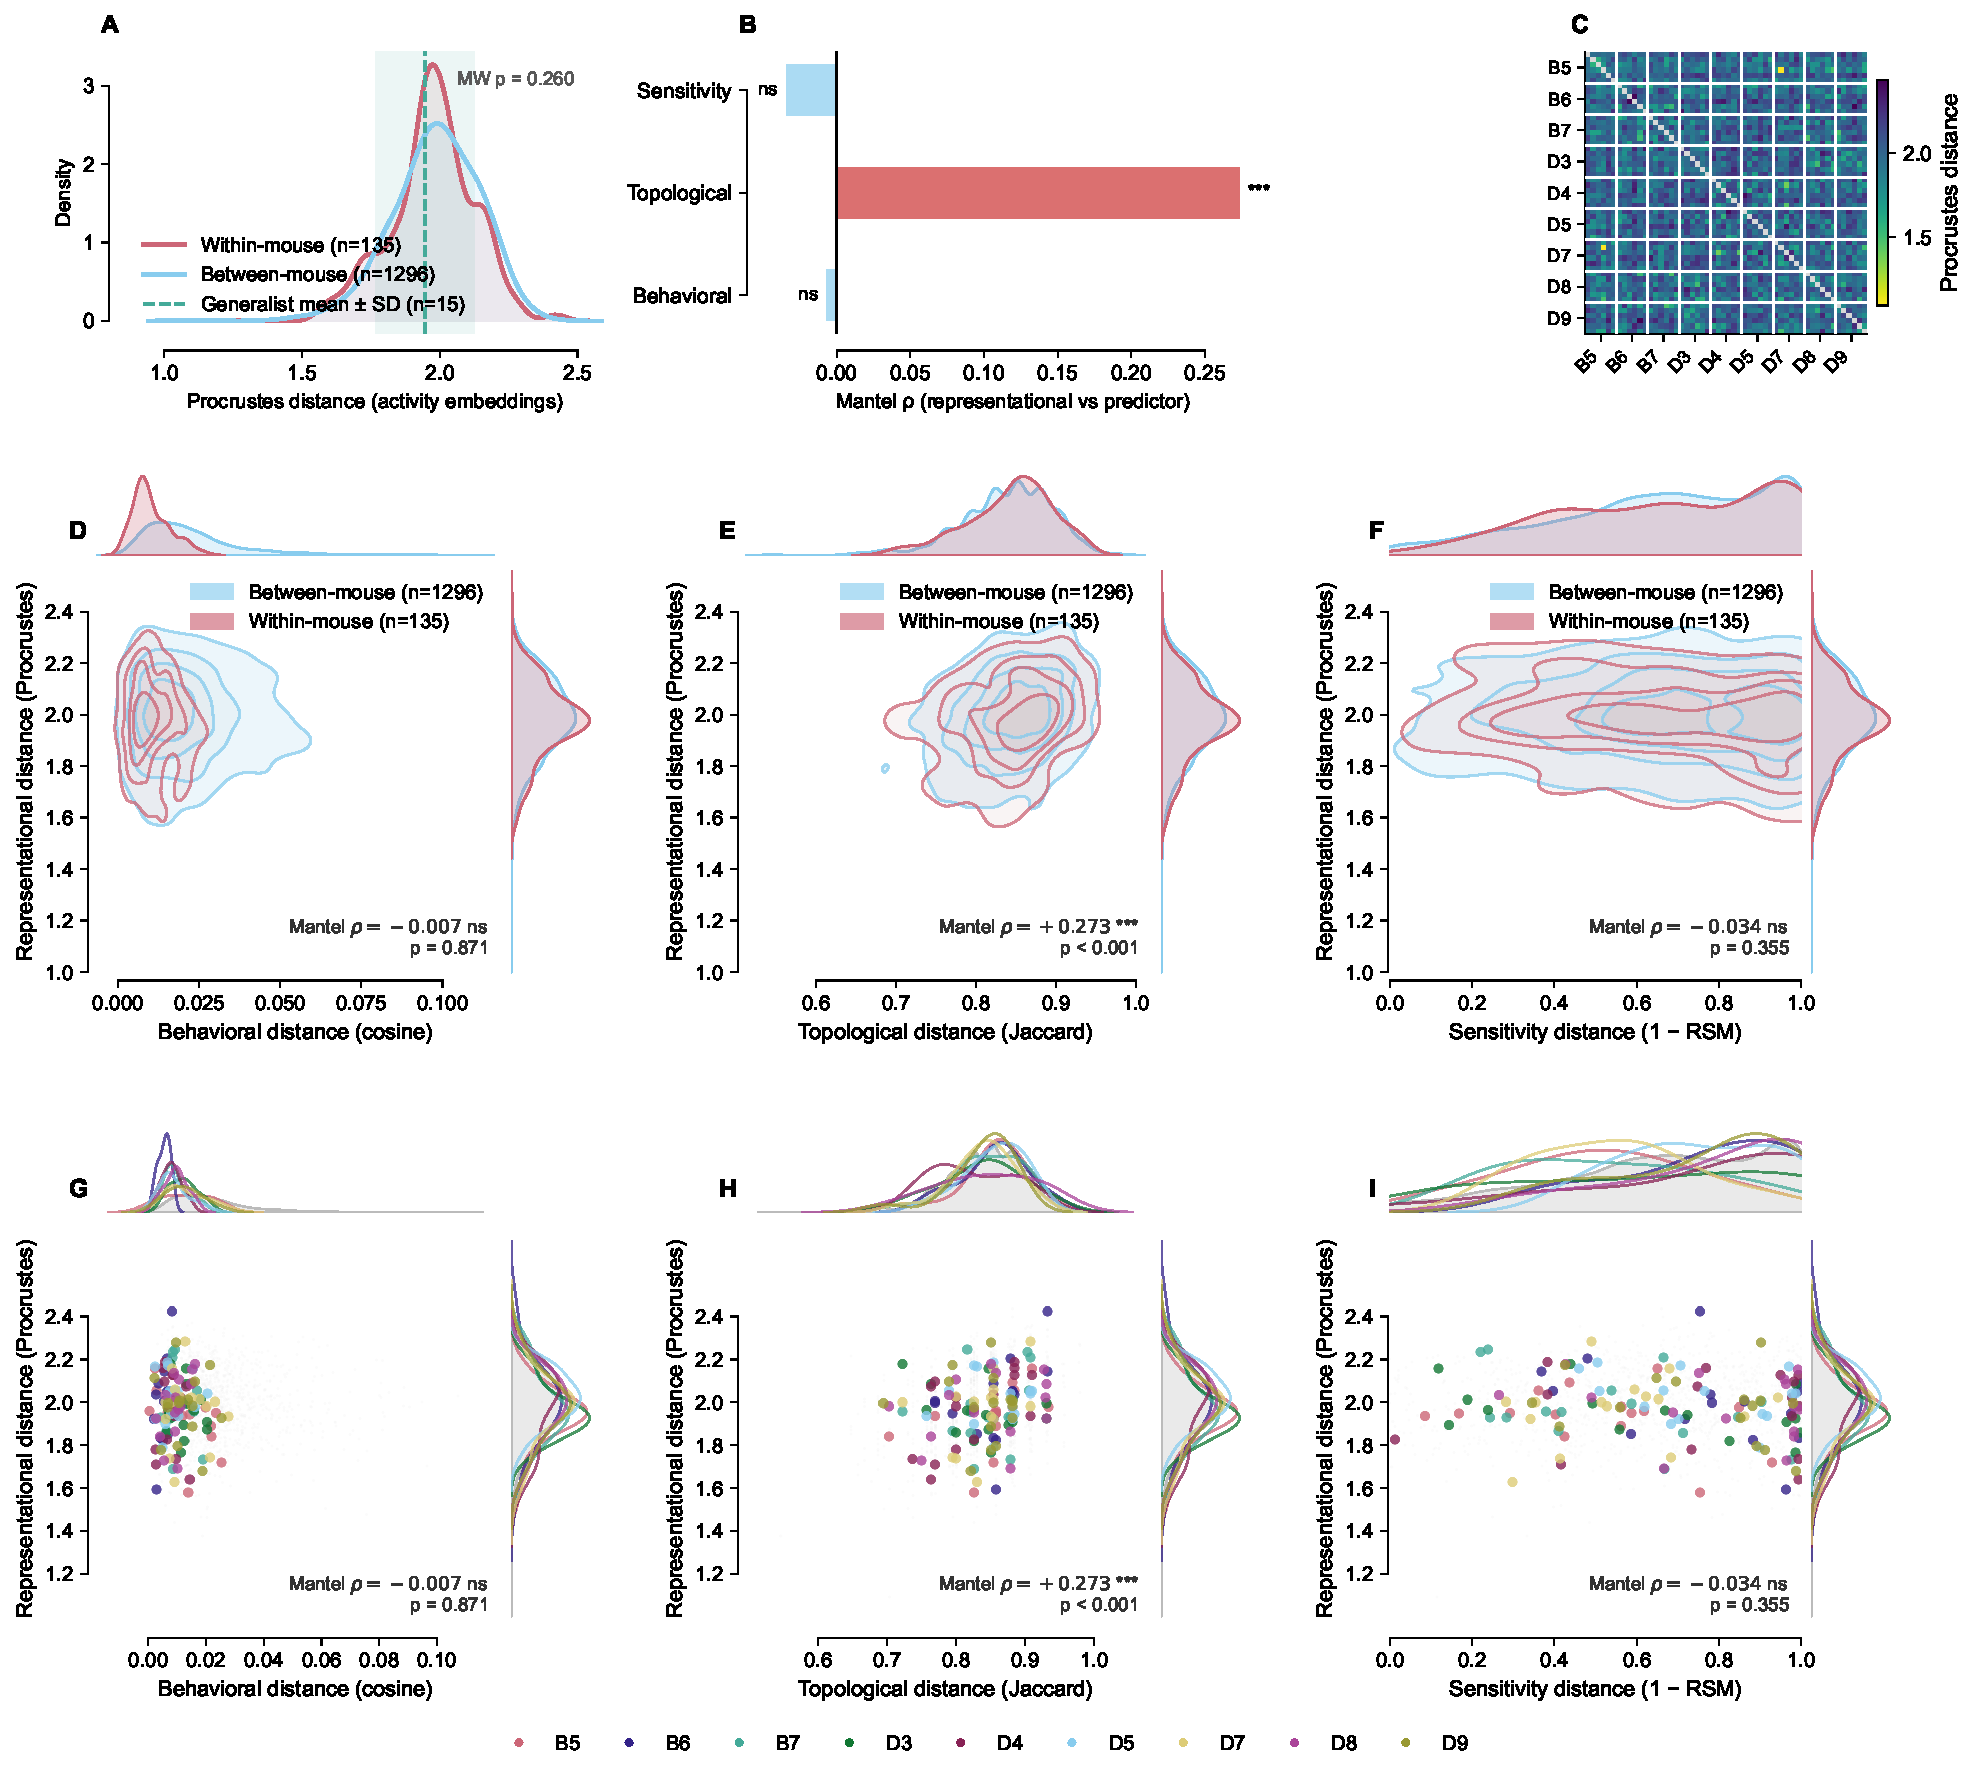
\includegraphics[width=\textwidth]{fig_embedding_rsa_v2.pdf}
  \caption{\textbf{Representational geometry is degenerate across levels.}
  (A)~Procrustes distance between PC loading matrices (activity embeddings), within-mouse
  pairs (red, $n=135$) versus between-mouse pairs (blue, $n=1{,}296$). Dashed line and
  shaded band show generalist mean $\pm$ SD ($n=15$). Distributions are
  indistinguishable (MW $p = \statActEmbRsaMwP$), confirming that individual-target
  selection produces no convergence in embedding space.
  (B)~Mantel $\rho$ between representational distance and three candidate predictor
  distances (behavioral, topological, sensitivity). Red bars indicate significant results;
  only topological distance is significant ($\rho = \statActEmbTopoMantelRho$, $p < 0.001$,
  \textasteriskcentered\textasteriskcentered\textasteriskcentered), in the expected
  \emph{positive} direction: circuits sharing more topological scaffold tend toward
  slightly more similar representations. Behavioral and sensitivity correlations are null
  ($\rho = \statActEmbBehMantelRho$ and $\rho = \statActEmbSensMantelRho$, both $p > 0.3$, ns).
  (C)~$54 \times 54$ Procrustes distance matrix, agents sorted by mouse identity (white lines
  mark $6 \times 6$ group boundaries). Absence of darker blocks on the diagonal confirms no
  within-mouse convergence in representational space.
  (D--F)~KDE joint plots of representational distance versus behavioral (D), topological (E),
  and sensitivity (F) distances for all $1{,}431$ agent pairs. Within-mouse (red) and
  between-mouse (blue) contours overlap on all three axes; Panel~E reveals the only
  significant relationship ($\rho = \statActEmbTopoMantelRho$, $p < 0.001$).
  (G--I)~Same three axes as D--F, with between-mouse pairs shown in grey and within-mouse
  pairs coloured by individual mouse identity (legend below). No mouse's replicates
  cluster at distinctively lower representational distances, confirming that representational
  degeneracy holds at the level of individual mice.}
  \label{fig:embedding_rsa}
\end{figure}


% ---------------------------------------------------------------------------
\subsection{Dynamical geometry is also degenerate}
\label{sec:dynamics_degen}
% ---------------------------------------------------------------------------

The structural degeneracy established in Sections~\ref{sec:paradox}--\ref{sec:sensitivity}
is most starkly illustrated at the level of individual circuit pairs.
Figure~\ref{fig:circuit_comparison}A shows the positions of two within-mouse pairs
within the full topology-behaviour landscape: both lie at near-zero behavioural distance
yet are separated by the full topological range of the dataset (pair~1 at the minimum
within-mouse Jaccard distance, pair~2 at the maximum).
The most topologically similar within-mouse pair in the dataset (mouse~\statCircSimMouse,
replicates~2 and~5; Jaccard distance $= \statCircSimJaccard$) shares only
$\statCircSimSharedEdges$ of $\statCircSimUnionEdges$ edges
(\statCircSimSharedFracPct\%), yet achieves a behavioural distance of
$\statCircSimBehDist$, effectively producing identical navigation fingerprints.
The most topologically dissimilar within-mouse pair (mouse~\statCircDisMouse,
replicates~1 and~5; Jaccard $= \statCircDisJaccard$) shares only
$\statCircDisSharedEdges$ of $\statCircDisUnionEdges$ edges
(\statCircDisSharedFracPct\%), and achieves an equally close behavioural match
($\statCircDisBehDist$).
These two circuits employ architecturally distinct motifs:
replicate~1 concentrates connectivity in the recurrent interneuron layer
($\statCircDisRepOneSensInter$ sensory$\to$interneuron,
$\statCircDisRepOneInterInter$ interneuron$\to$interneuron,
$\statCircDisRepOneInterMotor$ interneuron$\to$motor connections),
while replicate~5 shifts to broader sensory integration with reduced recurrence
($\statCircDisRepFiveSensInter$, $\statCircDisRepFiveInterInter$, $\statCircDisRepFiveInterMotor$).

\begin{figure}[H]
  \centering
  \captionsetup{width=\textwidth}
  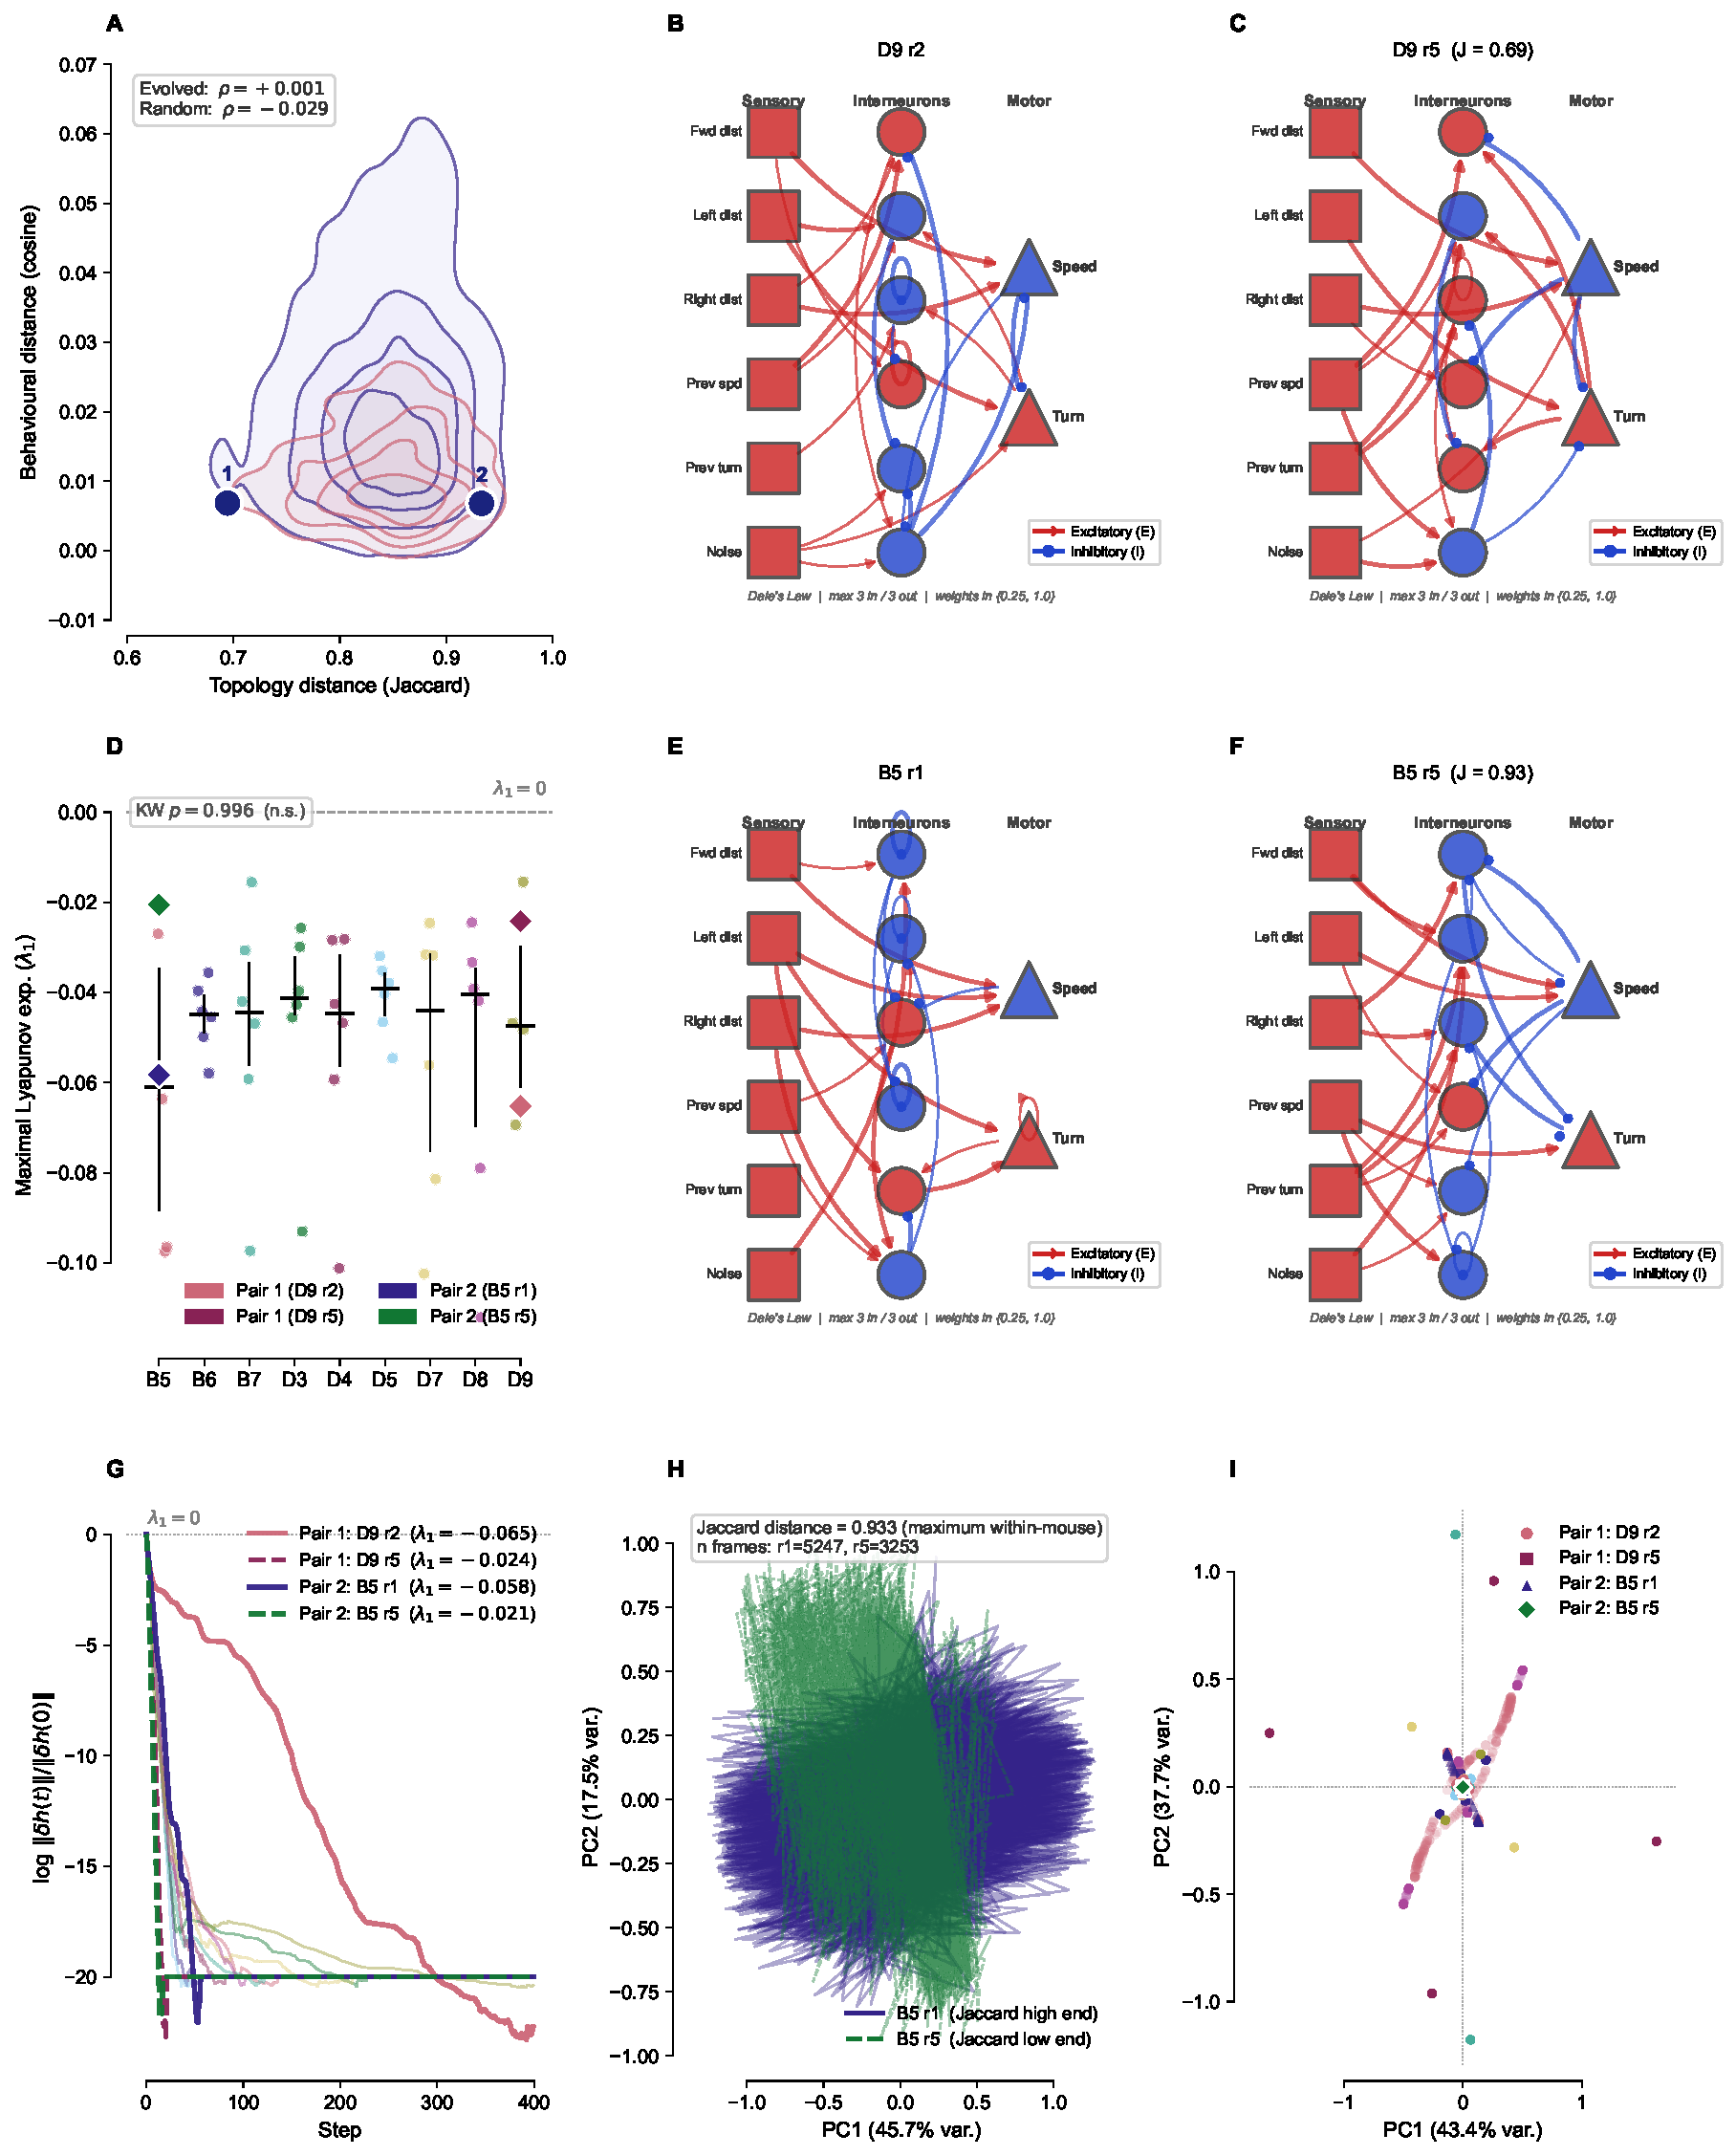
\includegraphics[width=\textwidth]{fig_circuit_comparison.pdf}
  \caption{\textbf{Structural and dynamical degeneracy: topology-disparate circuits are
  behaviourally and dynamically indistinguishable.}}
  \label{fig:circuit_comparison}
\end{figure}

\clearpage
\begin{figure}[H]\ContinuedFloat
  \caption*{%
    \textbf{Structural and dynamical degeneracy contd...}
    (A)~Joint KDE contours of topology Jaccard distance versus behavioural cosine
    distance for all $1{,}431$ evolved agent pairs (within-mouse: rose; between-mouse: indigo).
    Numbered dots mark the two within-mouse pairs selected for circuit comparison:
    \textbf{1}~is the most topologically similar pair
    (mouse~\statCircSimMouse, Jaccard $= \statCircSimJaccard$);
    \textbf{2}~is the most topologically dissimilar
    (mouse~\statCircDisMouse, Jaccard $= \statCircDisJaccard$).
    Both lie at near-zero behavioural distance despite spanning the full topological range.
    \textbf{(B, C)}~Circuit diagrams for pair~1 replicates (\statCircSimMouse{} r2 and r5).
    \textbf{(D)}~Per-mouse maximal Lyapunov exponent $\lambda_1$ for all 54 agents (strip plot
    with median and IQR); diamond markers indicate the four selected agents; dashed line at
    $\lambda_1 = 0$; Kruskal-Wallis $p = \statDynamicsLyaKwP$ (n.s.).
    \textbf{(E, F)}~Circuit diagrams for pair~2 replicates (\statCircDisMouse{} r1 and r5).
    Node colours: sensory (squares, blue/red by Dale type), interneuron (circles), motor
    (triangles). Edge colours: excitatory (red), inhibitory (blue).
    \textbf{(G)}~Perturbation decay curves ($\log\|\delta h(t)\|/\|\delta h(0)\|$):
    per-mouse means across all six replicates (thin lines, nine mouse colours) with
    four selected circuits overlaid in bold; $\lambda_1$ values annotated.
    All circuits collapse toward the same stable regime, with individual trajectories
    lying within the population envelope.
    \textbf{(H)}~Driven trajectory PCA for pair~2 (\statCircDisMouse{} r1 and r5):
    interneuron and motor activations (dims 6--13) from all valid maze bouts projected
    to a shared 2-D PCA. The two circuits -- separated by the maximum within-mouse
    topology distance (Jaccard $= \statCircDisJaccard$) -- trace overlapping
    trajectories, confirming that trajectory-level degeneracy is topology-independent.
    \textbf{(I)}~Autonomous attractor terminal states: all 54 evolved agents run from
    200 random initial conditions for 500 steps under zero sensory drive; terminal
    states projected to a shared 2-D PCA (interneuron and motor dims, colour-coded by
    mouse). The four selected circuits are highlighted (pair~1: \statCircSimMouse{}
    r2 and r5; pair~2: \statCircDisMouse{} r1 and r5). Population-wide convergence
    to a common attractor region supports the absence of mouse-specific stability
    signatures.}
\end{figure}

Extensive structural heterogeneity does not produce corresponding heterogeneity in
dynamical character.
The maximal Lyapunov exponent $\lambda_1$, estimated for all 54 agents via finite
perturbation (Section~\ref{sec:methods_dynamics}), was negative for every agent
(grand mean $\lambda_1 = \statDynamicsLyaMean \pm \statDynamicsLyaStd$,
range $[\statDynamicsLyaMin,\, \statDynamicsLyaMax]$), establishing a uniform
slightly-stable dynamical regime across the population.
One-way ANOVA across mice returned $F = \statDynamicsLyaF$, $p = \statDynamicsLyaP$;
Kruskal-Wallis confirmed the null ($H = \statDynamicsLyaKwH$, $p = \statDynamicsLyaKwP$):
no mouse-specific stability signature exists, despite topological distances
spanning the full range from $\statCircSimJaccard$ to $\statCircDisJaccard$
(Figure~\ref{fig:circuit_comparison}D, G).

The degeneracy extends to autonomous dynamics.
Each agent was run from 200 random initial conditions under zero sensory drive for
500 steps; virtually all agents converged to a single fixed-point attractor,
with no within-versus-between-mouse difference in attractor landscape
(sliced Wasserstein distance: within $\statActEmbAttrWithinWass \pm \statActEmbAttrWithinWassStd$
versus between $\statActEmbAttrBetweenWass \pm \statActEmbAttrBetweenWassStd$;
Mann-Whitney $p = \statActEmbAttrMwP$;
Figure~\ref{fig:circuit_comparison}I).

Driven activity trajectories are likewise degenerate.
All 54 agents were presented with an identical 1000-step standardised sensory sequence
(Section~\ref{sec:methods_dynamics}); pairwise cosine similarity of mean activation
trajectories showed no within-mouse elevation
(Mann-Whitney $p = \statDynamicsTrajectoryP$;
Supplementary Figure~\ref{fig:supp_dynamics_null}B; Figure~\ref{fig:circuit_comparison}H for
the pair-level trajectory PCA).

Across all three dynamical assays, stability regime, attractor landscape, and
driven activity geometry, the circuits are indistinguishable.
The architectural motif differences visible in Figure~\ref{fig:circuit_comparison}
(recurrence-heavy versus sensory-integration-heavy wiring) do not produce different
dynamical regimes.
Degeneracy in this system therefore spans every level examined: aggregate statistics,
topology, causal sensitivity, representational geometry, and dynamical geometry.

% ============================================================================
\section{Discussion}
% ============================================================================

% ---------------------------------------------------------------------------
\subsection{Degeneracy in constrained circuits: pervasive, structurally
            invisible, functionally consequential}
\label{sec:disc_degeneracy}
% ---------------------------------------------------------------------------
%%% Synthesis -- not an introduction to degeneracy (that is now in Intro).
%%% Structure:
%%%   1. State the 4-level finding plainly
%%%   2. Contrast with Tononi 1999 (degeneracy + complexity)
%%%   3. Connect to Hu 2025 (extends to topology axis)
%%%   4. Connect to Huang 2024 (Contravariance -- inverted by architecture)
%%%   5. Functional sensitivity commitment as the positive claim

The central result of this study is a cautionary one for systems neuroscience:
behavioral individuation can be real and reliable yet invisible to the entire
standard toolkit for relating circuit structure to function. The nine individual
targets are genuinely distinguishable---a classifier separates them from the real
behavioral data alone at $\statIndividuationClassAccPct$\% accuracy against a
$\statIndividuationChancePct$\% chance level (Supplementary Analysis~\ref{sec:supp_holdout}),
and evolved specialisation persists on held-out trajectories---yet no aggregate
statistic, connection-topology measure, representational-similarity or manifold
analysis, or attractor/Lyapunov descriptor recovers which mouse a circuit was shaped
to become. An analyst equipped with the methods most commonly used to characterise
neural circuits would conclude these circuits are interchangeable. They are not.

Our constrained system makes degeneracy an architectural fact rather than an inferred
property: the constraint geometry (Dale's Law, degree limits, quantized weights)
compresses all solutions into the same structural region regardless of the behavioral
target. This degeneracy has two faces, which we distinguish deliberately. At the level
of \emph{competence}, it is classical: the reachable structural space is saturated with
equally-good navigators, so selection is free to reach any of them (a many-to-one map
from structure to navigational fitness). At the level of \emph{identity}, it is stronger:
no structural axis distinguishes which mouse a circuit was shaped to replicate, even
though the individual behaviors differ. Individuation exists but leaves no structural
trace. We note that not all of the null results carry equal weight: some are close to
forced by the architecture. A small saturating \texttt{tanh} network under zero drive
contracts to a single stable fixed point, so the absence of a mouse-specific autonomous
attractor or Lyapunov signature (\S\ref{sec:dynamics_degen}) is largely guaranteed a
priori; the non-trivial dynamical test is the driven-trajectory comparison, which is
also flat. The structural, topological, and representational nulls are the substantive
ones, and it is their conjunction with demonstrable behavioral individuation that
constitutes the blind-spot result.

The identity-level degeneracy extends further than the aggregate floor. Connection
topology varies freely within and across mice, yet that variation carries no information
about behavioral identity at any scale: within mice, between mice, or across the full
agent population. The
mutual information between any structural axis and behavioral identity is weak and
non-significant (maximum NMI $= \statDegAthreeNmiMax$). And critically, this
topology-behavior flatness is architectural rather than a product of selection: random
constrained agents show the same flat relationship as evolved ones
($\rho_\text{random} = \statDegAfiveRhoRand$, $p = \statDegAfivePRand$). Selection
does not create the degeneracy; the architecture does. Selection operates within it.

This extends and deepens earlier work on degeneracy in evolved artificial agents.
\citet{hu2025degeneracy} demonstrated degeneracy at behavioral, structural, and
computational levels in Markov brain agents, and showed that it can arise in
systems not explicitly designed for it. Our results push this further: in the
extreme-constraint regime of 14 neurons, quantized weights, and Dale's Law,
degeneracy operates even on the topology axis itself, the level at which one
might most naturally expect individual identity to be encoded. There is no unique
``mouse-B5 topology'': the fitness landscape is many-to-one across the entire
topological space accessible to the constrained architecture.

\citet{tononi1999measures} showed empirically that degeneracy and neural complexity
are positively correlated: more degenerate systems tend to be more complex, because
degeneracy enables diverse responses to diverse stimuli through a shared structural
substrate. Our results are consistent with this picture at the aggregate level but
reveal an additional dimension: degeneracy can be present and pervasive even when
structural axes are entirely uninformative about behavioral identity. The absence of
structural signal does not mean the absence of functional differentiation; it means
the differentiation lives somewhere else.

Where it lives is in functional sensitivity commitment. \citet{huang2024degeneracy}
(preprint) propose a Contravariance Principle: increasing task complexity reduces
dynamical degeneracy, because more complex tasks impose tighter constraints on the
solution space. Our system inverts this logic by imposing constraint from the architecture
rather than the task, and shows that when the architecture saturates the
structural axes, selection routes behavioral individuation through a functional
channel (sensitivity commitment) that leaves no structural trace. Specialists
develop high, varied sensitivity to circuit perturbations, but not convergent:
within-mouse sensitivity profiles are no more similar than between-mouse profiles
($\statClaimTwentyEightWithinSim$ versus $\statClaimTwentyEightBetweenSim$; the small
gap is not significant under a pseudoreplication-aware test,
label-permutation $p = \statClaimTwentyEightPermP$), so even replicates of a single mouse
do not converge on a shared sensitivity signature. Generalists show substantially lower,
more uniformly distributed sensitivity ($\bar{\sigma}^2 = \statDegAsixGenSensVarMean$)
with no strong commitment to any subset of pathways. The
$\statDegAsixVarRatioWithin$--$\statDegAsixVarRatio\times$ difference in sensitivity variance between specialists
and generalists (mouse-level $p = \statDegAsixMouseWilcoxP$) is the signature of what
individual-target selection achieves in a
degenerate space: functional commitment without structural differentiation, and
without convergence on specific pathways.
The representational and dynamical geometry analyses confirm that this absence of
convergence is complete: activity embedding geometry
(§\ref{sec:rep_geometry}) and dynamical regime
(§\ref{sec:dynamics_degen}) are equally uninformative about mouse identity.
Functional sensitivity commitment is the only dimension along which
individual-target selection leaves a detectable trace in this system.


% ---------------------------------------------------------------------------
\subsection{The role of architectural constraints}
\label{sec:disc_constraints}
% ---------------------------------------------------------------------------
%%% Largely retained from v1 sec 3.2.
%%% Remove: "topology is the non-degenerate axis" language.
%%% Replace with: topology is computational substrate but not individuating axis.

Structural convergence in our system reflects an architectural floor rather than an
evolved property: randomly initialised constrained agents return an identical 0/18
significant structural features to evolved agents. The degree limit, quantized
weights, and Dale's Law together reduce the space of realisable circuits so tightly
that no aggregate feature can diverge across populations regardless of training.
Evolution's contribution is not convergence of structure (which would happen
anyway) but convergence of function: finding computationally specific wiring
configurations within that compressed structural space that replicate individual
behavioral signatures.

The binary weight scheme $\{0.25, 1.0\}$ imposes an analogous compression at the
magnitude level. With at most 3 connections per source and only two magnitude
values, $\statMagnitudeDegeneracyEvolvedFrac$\% of source neurons carry uniform
magnitude assignments that are unaffected by shuffling. Magnitude is therefore
a doubly degenerate axis: it carries no information about behavioral identity
(NMI $= \statDegAthreeNmiMag$) and is causally interchangeable (magnitude
permutation reduces MSE rather than elevating it). The architecture forces all
variation that matters to live in the one causally potent axis it leaves free: the
specific pattern of who-connects-to-whom.

But causal potency is not the same as informational sufficiency. Topology is causally necessary: permuting
connection targets disrupts computation ($\statDynamicsPermOverReplicate\times$ MSE
increase). But topological variation is degenerate with respect to behavioral
identity: the specific topology an agent uses carries no information about which
mouse it was trained on. The architecture makes topology the only axis with causal
weight; the fitness landscape makes that axis informationally flat. Selection
navigates this constraint by shaping functional sensitivity structure rather than
topological pattern.
The representational geometry analysis (§\ref{sec:rep_geometry}) confirms that this
structural floor propagates through to the activity level: topology predicts
activity embedding geometry (Mantel $\rho = \statActEmbTopoMantelRho$, $p < 0.001$),
confirming that structure does constrain dynamics, but too weakly and non-specifically
to fingerprint behavioral identity at the individual-mouse level.


% ---------------------------------------------------------------------------
\subsection{Implications for neural coding}
\label{sec:disc_coding}
% ---------------------------------------------------------------------------
%%% Largely retained from v1 sec 3.3.
%%% Add: paragraph connecting functional sensitivity commitment to biological
%%%      circuit individuation literature.

Our results suggest that aggregate circuit statistics (the metrics most commonly
used to characterise neural circuit organisation) may be insufficient to capture
functional differences between individuals. Two circuits can have identical aggregate
structural profiles (pathway counts, weight magnitudes, E/I composition) while being
specialised to distinct behavioral targets. This has direct implications for
connectomics efforts that aim to relate circuit structure to function: the mapping
from structure to function is many-to-one---many structurally distinct circuits realise
the same competence (navigational fitness)---and, more strongly, structure additionally
fails to encode \emph{which individual} a circuit implements. We demonstrate this
many-to-one, identity-degenerate direction directly; we do not claim the converse
plurifunctional (one-structure-to-many-functions) direction, which our design does not
test. This matters most in systems where architectural constraints compress the
structural space \citep{bargmann2013connectome, jonas2017microprocessor}.

The per-source ablation null result (0 of 14 source neurons significant; within-mouse
sensitivity profiles no more correlated than between-mouse profiles) extends this to
the local level. No single neuron bears disproportionate responsibility for
mouse-specific calibration. This holistic distribution parallels ensemble coding in
biological systems, where behaviorally relevant information is encoded in distributed
patterns of neural activity rather than in the firing of any individual cell
\citep{georgopoulos1986neuronal}. Consistent with this principle, no individual neuron carries disproportionate
responsibility for behavioral calibration in our system. Causal weight is
distributed across the circuit topology, yet that distributed pattern is itself
degenerate across agents.

The functional sensitivity commitment result (A6) suggests a specific prediction for
biological circuits. If the principle generalises, one would expect circuits evolved
or trained for individual-specific behavioral targets to show higher, more consistent
sensitivity to perturbations of particular pathways than circuits optimised for
population-level or multi-target performance, even when the circuits are
structurally indistinguishable by any aggregate measure.
The representational degeneracy result (§\ref{sec:rep_geometry}) deepens this
prediction: functional individuation leaves no trace even in the geometry of neural
activity embeddings, suggesting that population-activity analyses commonly used
in systems neuroscience (manifold dimensionality, cross-session RSA, CKA)
may be systematically insensitive to individual-specific circuit organisation
even when that organisation is strong. Measuring functional sensitivity commitment
(rather than structural or representational similarity) may therefore be a more
productive strategy for identifying individual-specific circuit organisation in
biological neural systems.


% ---------------------------------------------------------------------------
\subsection{Limitations}
\label{sec:disc_limitations}
% ---------------------------------------------------------------------------
%%% Largely retained from v1 sec 3.4.
%%% Add: A4 power note (underpowered for sensitivity RSA geometry;
%%%      planned follow-up with additional replicates).

Several limitations apply. First, the quantized weight scheme ($\{0.25, 1.0\}$)
limits the resolution of synaptic strength tuning. Continuous weights might reveal
more pathway-level magnitude variation and could alter the topology-vs-magnitude
result, which may partly reflect the architecture's unusually compressed magnitude
space rather than a general principle \citep{huang2024degeneracy}.

Second, the fitness function captures behavioral statistics rather than
moment-by-moment trajectory matching, and the behavioral fingerprint (4 metrics from
maze navigation) may not represent all relevant dimensions of individual mouse
identity. Other behavioral contexts, additional metrics, or richer trajectory
representations might reveal structural signals invisible to the current fitness
function.

Third, the 14-neuron network is a deliberate minimal model. Real navigation circuits
in rodents involve millions of neurons across hippocampus, entorhinal cortex, and
striatum. Whether topology-dominant causal encoding and functional sensitivity
commitment as the individuating property scale to larger, biologically realistic
networks is an open question. Degeneracy and neural complexity are empirically
positively correlated \citep{tononi1999measures}, suggesting structural convergence
may become more pronounced in larger networks; the topology-behavior flatness we
observe, however, emerges already in the minimal 14-neuron case and is architectural
rather than size-dependent.

Fourth, the sensitivity RSA analysis (A4) is likely underpowered in the current
dataset. The Mantel test and within/between MW statistic are both null (Mantel
$\rho = \statDegAfourMantelRho$, permutation $p = \statDegAfourMantelPPerm$), but
with 54 agents across 9 mice the geometric resolution of the 14-dimensional
sensitivity space is limited. Whether the \emph{geometry} of the sensitivity profile
(as opposed to its variance) carries individual-specific information at higher
replicate counts remains an open question. Additional replicates (targeting $n = 10$
per mouse) are planned.

Fifth, results are drawn from 9 mice across two inbred strains navigating a single
maze geometry without reward. Generalisation to outbred populations, different maze
conditions, or different task structures requires further investigation. These
findings constitute a proof-of-concept demonstration in a controlled minimal system,
not a general claim about neural coding mechanisms.

Sixth, the analysis is null-heavy by design, and the interpretation rests on a small
number of positive results, each tied to a specific pre-specified hypothesis rather
than emerging from an unstructured screen: the topology-to-representation correspondence
(Mantel $\rho = \statActEmbTopoMantelRho$, $p = \statActEmbTopoMantelP$) and the
specificity dose-response (Spearman $\rho = \statPermutationOptionaSpearmanRho$,
permutation $p = \statPermutationOptionaSpearmanPermP$, $n = 9$). We report these with
effect sizes and confidence intervals rather than $p$-values alone, and do not apply a
joint multiple-comparison correction across them because they test distinct,
independently motivated hypotheses. The dose-response in particular is borderline and,
as noted above, indicative rather than firmly established; neither the causal nor the
representational conclusion depends on it.


% ---------------------------------------------------------------------------
\subsection{Future directions}
\label{sec:disc_future}
% ---------------------------------------------------------------------------

Several extensions would strengthen and generalise these findings. First, increasing
replicates to 10--15 per mouse would provide adequate power for the sensitivity RSA
geometry analysis (A4) and would also improve resolution on medium-effect structural
features. This is tractable within the current evolutionary framework.

Second, relaxing architectural constraints, i.e.\ allowing more connections per neuron,
continuous weights, or removing Dale's Law, would test whether the topology-behavior
flatness and functional sensitivity commitment results depend on the extreme-constraint
regime or persist across a wider range of architectures. The representational
(§\ref{sec:rep_geometry}) and dynamical (§\ref{sec:dynamics_degen}) geometry analyses
provide additional comparison axes: whether representational and dynamical degeneracy
persist in less constrained circuits, or whether structural signal propagates through
to activity geometry and stability regime at higher architectural complexity.

Third, the generalist result (Section~\ref{sec:sensitivity}) opens a productive
experimental direction: training agents on subsets of mice (2, 3, or 4 targets)
would allow systematic characterisation of how functional sensitivity commitment
degrades as a function of the number of behavioral targets, and at what point
individual-target specificity becomes impossible to maintain.

Fourth, applying the same framework to other behavioral datasets, i.e.\ different
species, tasks, or maze geometries, would test whether functional sensitivity
commitment as the individuating property is specific to mouse navigation or a more
general consequence of individual-target optimisation in constrained circuit spaces.

Finally, bridging to real neural recordings would test the biological relevance of
the mechanisms identified here. The computational circuit predicts that
individually-calibrated circuits should show higher functional sensitivity commitment
than population-optimised ones, even when structurally indistinguishable. This
prediction is testable using perturbation experiments (optogenetic or pharmacological
silencing of identified pathway types) combined with behavioral readout in animals
with known individual behavioral profiles.


\section*{Methods}
% ----------------------------------------------------------------------------

\subsection{Mouse behavioral data}

We used behavioral data from 9 mice (B5, B6, B7, D3, D4, D5, D7, D8, D9) exploring a
hierarchical binary tree maze without reward, from \citet{rosenberg2021mice}. For each mouse, we
computed four behavioral metrics from the raw trajectory data:
\begin{enumerate}
  \item Transition probabilities between maze arms (Markov property): Decision-making at various nodes in the binary tree representing the maze can be characterised with a Markov-chain analysis. For each node in the maze, we compute the probability distribution over next-node transitions based on the direction of entry (from the bottom, left or right arm), and that of left versus right, yielding a 6-dimensional vector per node. These are averaged across a level and stacked across the tree, both for the agent and the mouse. The Euclidean distance between these bias profiles becomes the penalty for the agent.
  \item Spatial occupancy as a node-visit distribution: A probability distribution over the maze's corridor nodes (runs) is constructed by weighting each node proportionally to the total number of frames the mouse spent there within a bout. Dwell time for each node is computed as the difference between consecutive start-frame entries in the Rosenberg bout traces, matching the reference implementation of \citet{rosenberg2021mice}. The Jensen-Shannon divergence between the agent and mouse node-occupancy distributions is applied as a penalty, encouraging the agent to explore the maze with similar spatial coverage as the mouse.  \item Path tortuosity: Path efficiency is measured using sliding window straightness. For each window, we compute the ratio of the displacement to distance. A penalty is applied according to relative deviation from the mouse baseline. 
  \item Turn bias: A simple turn bias (left versus right) is calculated using the distribution of angular velocities. The turn bias is the signed left--right asymmetry $(\text{n\_right} - \text{n\_left})/\text{n\_total} \in [-1, 1]$, and the agent is penalised for deviation from the mouse's turn bias.
\end{enumerate}
Simulated evaluation consists of 20 independent bouts of 2000 frames each.

\subsection{Network architecture}
\label{sec:network_arch}

Each agent is a recurrent neural network with 14 neurons: 6 sensory (front, left, right wall
distances; previous speed; previous turn rate; Gaussian noise), 6 interneurons, and 2 motor
(speed, turn rate). The network is updated at each timestep according to:
\begin{equation}
  h_j(t\!+\!1) = \tanh\!\Bigl(\sum_{i} W_{ij}\, h_i(t)\Bigr), \quad j \in \{\text{interneuron, motor}\}
\end{equation}
where $\mathbf{W}$ is the $14 \times 14$ weight matrix with $W_{ij}$ denoting the connection
from neuron $i$ to neuron $j$, and $\mathbf{h}$ is the state vector. In matrix notation,
$\mathbf{h}(t\!+\!1) = \tanh(\mathbf{W}^\top \mathbf{h}(t))$, equivalently
$\tanh(\mathbf{h}(t)^\top \mathbf{W})$ for $\mathbf{h}$ a row vector---the form
used in the reference implementation (\texttt{state @ W}), with $W_{ij}$ the weight
from $i$ to $j$ throughout.
Sensory neurons are clamped to their input values at each step; only interneuron and motor
states are updated dynamically.

Three biological constraints are enforced:
\begin{enumerate}
  \item \textbf{Dale's Law}: Each neuron is assigned a fixed type (excitatory or inhibitory).
    All outgoing weights share the source neuron's sign: $w_{ij} = |w_{ij}| \cdot \text{type}_i$.
    Sensory neurons are always excitatory (consistent with the predominantly glutamatergic
    nature of sensory afferents~\citep{kandel2021principles}); interneuron and motor types are evolved.
  \item \textbf{Sparse connectivity}: Each neuron has a maximum of 3 incoming and 3 outgoing
    connections. Sensory neurons receive no incoming connections. All other connection types
    are permitted: sensory$\to$interneuron, sensory$\to$motor, interneuron$\to$interneuron,
    interneuron$\to$motor, and motor$\to$interneuron (recurrent feedback). Self-connections
    (autapses) are permitted; empirically, $\statNetworkArchAutapsePct$\% of evolved agents
    ($\statNetworkArchAutapseN$ of $\statNetworkArchAutapseTotal$) acquired at least one
    self-connection on interneurons or motor neurons.
  \item \textbf{Quantized weights}: Magnitudes are drawn from $\{0.25, 1.0\}$. Combined with
    Dale's Law, the effective weights take values in $\{-1.0, -0.25, 0, +0.25, +1.0\}$.
\end{enumerate}

\subsection{Simulation environment}

The agent navigates a hierarchical binary tree maze rendered as a 2D polygon. At each timestep, sensory
inputs include 3 raycasts (front, left, right wall distances), previous speed, previous turn
rate, and noise ($\mathcal{N}(0, 0.1)$). Motor outputs are filtered through momentum dynamics:
\begin{align}
  v(t\!+\!1) &= (1 - \alpha_v) \, v(t) + \alpha_v \, v_\text{max} \, \tanh(m_\text{speed}) \\
  \omega(t\!+\!1) &= (1 - \alpha_\omega) \, \omega(t) + \alpha_\omega \, \omega_\text{max} \, \tanh(m_\text{turn})
\end{align}
where $\alpha_v = 0.263$ and $\alpha_\omega = 0.437$ are momentum coefficients, and $v_\text{max} = 1.949$ and
$\omega_\text{max} = 1.191$ are the maximum speed and turn rate, all derived empirically
from cross-subject medians of mouse trajectory statistics (lag-1 autocorrelations for speed
and turn rate; 99th-percentile speed and turn distributions; Gaussian smoothing
$\sigma = 1.0$ applied prior to parameter estimation). Full derivation details are provided
in Supplementary Methods. Each evaluation consists of 20 bouts of 2000 frames.

\subsection{Evolutionary algorithm}

We use a $(\mu + \lambda)$ evolutionary strategy with a population size of 500 and an elite
fraction of 10\% (50 agents). Three mutation operators are applied to offspring:
\begin{enumerate}
  \item Weight magnitude toggle (probability $p_w$): flips a connection's magnitude between
    0.25 and 1.0
  \item Structural rewiring (probability $p_s$): adds, removes, or redirects a connection
  \item E/I type flip (probability $p_n$): toggles a neuron between excitatory and inhibitory
\end{enumerate}
Mutation rates follow a linear decay from 15\% to 1\% over 200 total generations.
All results are reported at generation 150, where population fitness had plateaued in all
54 runs (defined as $<$2\% change across the final 30 generations); at this checkpoint the mutation
rate was approximately 4.5\%, which did not affect outcomes as fitness had plateaued by
generation 100--120 for all runs. The remaining 50 generations produced negligible improvement.
A connectivity repair step re-enforces structural constraints after each mutation:
(i) per-neuron degree limits (max 3 in/out) by pruning excess connections uniformly at random;
(ii) no incoming connections to sensory neurons; (iii) minimum 1
outgoing connection per non-motor neuron. Self-connections (autapses) are not prohibited
and frequently arise during evolution (see Section~\ref{sec:network_arch}).

\subsection{Fitness function}

Fitness is defined as:
\begin{equation}
  F = 2 \cdot \hat{M} + 2 \cdot \hat{O} + \hat{T} + \hat{B}
\end{equation}
where each component is normalized to $[0,1]$ using fixed reference constants derived from
the behavioral range of random agents: $\hat{M} = \min(1,\, d_{\mathrm{Eucl}}^{\mathrm{Markov}} / 6)$,
$\hat{O} = \min(1,\, d_{\mathrm{JS}}^{\mathrm{Occupancy}})$,
$\hat{T} = \min(1,\, |\Delta\text{tortuosity}| / \text{tortuosity}_\text{mouse})$, and
$\hat{B} = \min(1,\, |\Delta\text{turn bias}|)$.
The Occupancy component uses Jensen-Shannon divergence; the Markov component uses Euclidean distance between agent and target
bias profiles. Tortuosity and Turn bias use differences from target scalar values.
Lower fitness indicates a better match to the target mouse.
The 2$\times$ weighting on Markov and Occupancy reflects that these distributional measures
(JS divergence over decision-making transition patterns and spatial coverage) are richer in
individual-specific information than the scalar statistics captured by Tortuosity and Turn bias.
The sensitivity of this fitness function to individual mouse differences is validated by the
cross-mouse generalization result (Section~\ref{sec:paradox}): agents optimized for one mouse achieve
substantially higher fitness errors on other mice's behavioral profiles (off-diagonal mean
$\statCrossMouseOffMean \pm \statCrossMouseOffStd$ vs diagonal $\statCrossMouseDiagMean \pm \statCrossMouseDiagStd$).

\begin{figure}[H]
  \centering
  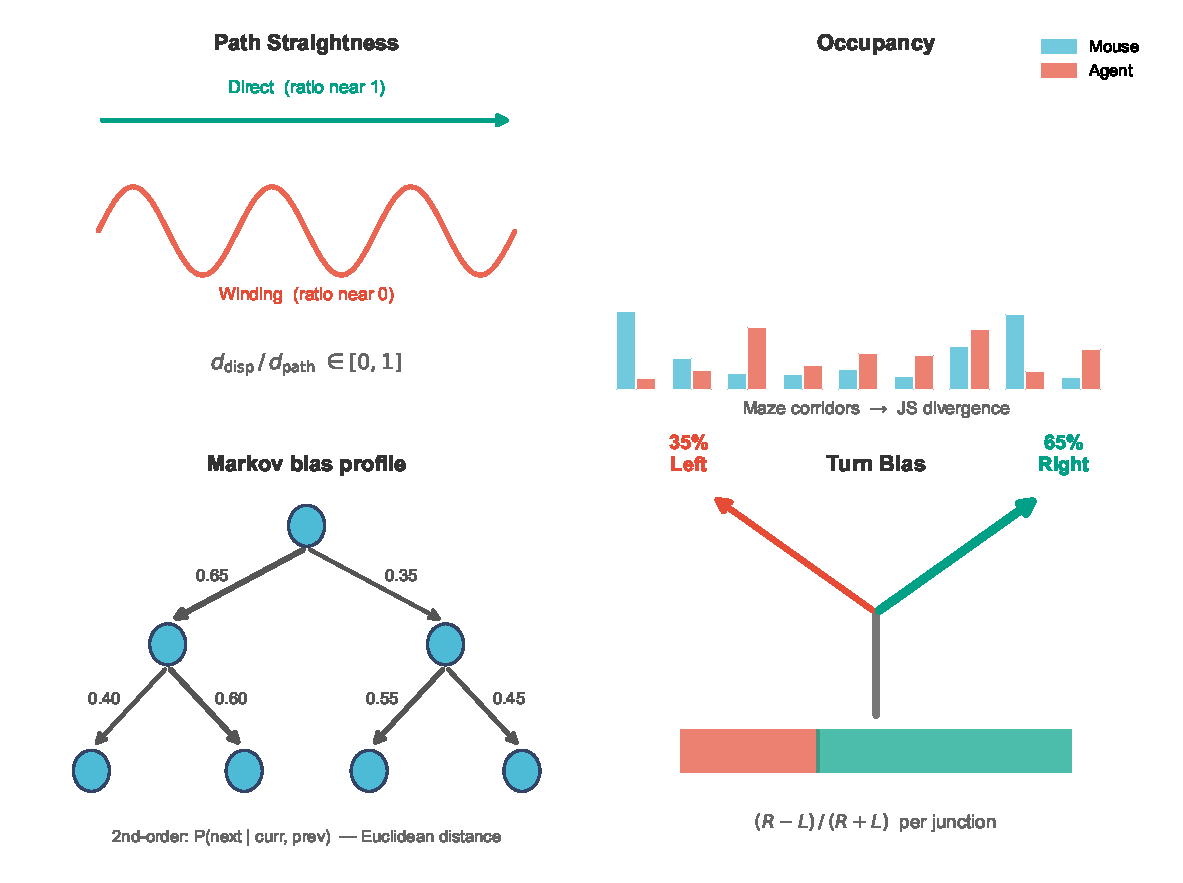
\includegraphics[width=0.65\textwidth]{fig_methods_fitness_metrics.pdf}
  \caption{\textbf{Behavioral fitness metrics.}
  The four components of the fitness function: transition probabilities (Markov bias
  profile), spatial occupancy (Jensen-Shannon divergence over node-visit distribution),
  path tortuosity (sliding-window straightness ratio), and turn bias (signed left--right
  angular velocity asymmetry). Each component is normalized to $[0,1]$ before weighting.}
  \label{fig:methods_fitness_metrics}
\end{figure}

\subsection{Circuit feature extraction}

For each of 54 best-evolved agents, we extracted 18 structural features spanning four
categories: connectivity (total connections, density), E/I composition (ratio,
excitatory/inhibitory counts), pathway counts (SI, SM, II, IM, MI, MM), E/I fractions per
pathway, interneuron degree statistics, and weight statistics (mean magnitude, fraction at
maximum). A baseline of 200 random agents was generated for comparison.

\subsection{Statistical analysis}

\paragraph{Per-mouse ANOVA.}
One-way ANOVA with Benjamini-Hochberg FDR correction ($\alpha = 0.05$) tested 18 features
across 9 mice ($k = 9$, $n = 6$ per group). Permutation tests (10,000 permutations) provided
non-parametric validation. BH-FDR was preferred over familywise-error correction (e.g., Bonferroni) because it controls the expected proportion of false discoveries rather than the probability of any false discovery, providing greater power for this discovery analysis across 18 features. The FDR guarantee holds under positive dependence among test statistics~\citep{benjamini1995controlling}, which applies here as pathway counts co-vary with total connection count. The null result is robust to correction method: although the smallest raw $p$-value is $\statAnovaTopFeatureP$ (interneuron fan-in), it does not survive correction ($p_\text{FDR} = \statAnovaTopFeaturePFdr$), the permutation test agrees ($p_\text{perm} = \statAnovaTopFeaturePPerm$), and no feature is significant after BH-FDR (0/18, all $p_\text{FDR} > \statAnovaMinPFdrFloor$).

\paragraph{Evolved vs random comparison.}
One-sample $t$-tests with Cohen's $d$ and bootstrap 95\% CIs (10,000 resamples).

\paragraph{Power analysis.}
Post-hoc power for the Wilcoxon signed-rank permutation specificity test ($n = 9$ paired
observations, one-tailed $\alpha = 0.05$) was computed via the normal approximation to the
Wilcoxon distribution. The observed effect size was Cohen's $d_z = \statPhaseThreecCohenDz$, yielding attained
power $> 0.999$. The minimum detectable effect at 80\% power was $d_z = \statPhaseThreecMdeD$ ($\statPhaseThreecMdeRaw$ fitness
units); the observed effect exceeds this threshold by a factor of $\statDerivedCohenDzOverMde$, making the $n = 9$
design adequate (Figure~\ref{fig:supp_power_curve}). For the circuit-level and structural
feature analyses, achieved power was computed via the non-central $F$ distribution and
minimum detectable $\eta^2$ was determined by binary search.

\paragraph{Cross-mouse generalization.}
A $9 \times 9$ fitness matrix was computed by evaluating each mouse's best agent on all 9
behavioral targets. The behavioral specialization index is defined as $1 -$ (diagonal mean /
off-diagonal mean); a value of 0 indicates no specialization, positive values indicate
specialization. The raw own/cross ratio equals $1 -$ index.

\paragraph{Strain clustering.}
Mann-Whitney $U$ test comparing within-strain vs between-strain off-diagonal fitness values.

\paragraph{Weight similarity.}
Pairwise cosine similarity of flattened weight matrices. Within-mouse vs between-mouse
comparison via Mann-Whitney $U$.

\paragraph{Activation trajectory analysis.}
All 54 best agents were run on an identical 1000-step standardized sensory input sequence
(random seed fixed at 42). Only the three wall-distance inputs ($d_f$, $d_l$, $d_r$) follow
a sinusoidal profile; the speed and turn proprioceptive inputs are derived from the agent's
own motor outputs at each step (closed-loop feedback), consistent with how agents operate
during actual maze navigation. This sequence does not come from actual maze trajectories; it
is a synthetic standardized probe designed to elicit comparable dynamics across all agents. Hidden-unit
states (8 dimensions: 6 interneurons + 2 motors) were recorded at each timestep.

Two representational similarity matrices (RSMs) were computed: (1) pairwise cosine similarity
of per-agent mean activation vectors, and (2) mean pairwise Pearson correlation across all 8
dimensions of the full 1000-step trajectory. Within- vs between-mouse similarity was compared
via Mann-Whitney $U$ (one-sided, $\alpha = 0.05$). PCA was applied to mean activation vectors
for visualization.

Maximal Lyapunov exponents were estimated for all 54 agents via finite perturbation
($\varepsilon = 10^{-6}$, 8 random unit-vector perturbation directions). Log divergence
$\Lambda(t) = \log(\|\mathbf{h}(t) - \mathbf{h}_\varepsilon(t)\| / \varepsilon)$ was tracked
for 400 steps; $\lambda_1$ was estimated as the mean log-divergence rate over the full
400-step trajectory (Equation~\ref{eq:lyapunov}), averaged over the 8 perturbation directions.
One-way ANOVA and Kruskal-Wallis tests compared $\lambda_1$
across mice.

\paragraph{Fixed point analysis.}
For each agent's 8$\times$8 autonomous submatrix
$\mathbf{W}_\text{sub} = \mathbf{W}_{[6:14, 6:14]}$ (interneurons and motors under zero
sensory drive, i.e.\ the circuit's intrinsic attractor structure independent of input),
fixed points were found via iterative
convergence ($h \leftarrow \tanh(\mathbf{W}_\text{sub}^\top h)$, 300 random restarts, tolerance
$10^{-5}$, maximum 5000 iterations), consistent with the forward-pass convention
$h_j = \tanh(\sum_i W_{ij} h_i)$. Duplicate fixed points were removed at distance
$< 10^{-3}$.

The Jacobian at each fixed point was computed as
$\mathbf{J} = \mathrm{diag}(1 - (\mathbf{h}^*)^2) \cdot \mathbf{W}_\text{sub}^\top$, and the
dominant eigenvalue $|\lambda_\mathrm{max}|$ was obtained via
\texttt{scipy.linalg.eigvals}. One-way ANOVA and Kruskal-Wallis tests compared fixed point
count and $|\lambda_\mathrm{max}|$ across mice.

\paragraph{Weight permutation ablation.}
For each of 54 agents, 20 permuted variants were generated using a source-preserving scheme.
Within each of 6 pathway blocks (SI, SM, II, IM, MI, MM), we permuted only which target
neurons each source connects to, keeping per-source out-degree, weight magnitudes, and Dale's
Law sign fixed. By \emph{connection topology} we mean precisely this assignment of
source-to-target pairs within each pathway block: which $k$ of the available target neurons
each source connects to, given fixed out-degree, Dale's Law sign, and weight magnitudes. This
is distinct from graph-theoretic topology (cycle structure, path lengths, spectral properties),
which is preserved by construction since the degree sequence and block structure are unchanged.
This preserves all 18 structural features exactly, including E/I fractions per pathway block.

Each evolved agent's permutation space is large: the mean number of distinct connectivity
assignments consistent with the structural constraints is
$10^{\statPermSpaceLogConfigsMean}$ configurations
(range $10^{\statPermSpaceLogConfigsMin}$--$10^{\statPermSpaceLogConfigsMax}$
across 54 agents; Supplementary Analysis).
Of source-pathway combinations, $\statPermSpaceFracNontrivialPct$\% have non-trivial
permutation freedom ($>$1 available target assignment).
Sensory-to-interneuron connections carry the most freedom
(SI: mean $C = \statPermSpaceChoicesSiMean \pm \statPermSpaceChoicesSiStd$ choices per source);
motor-target pathway blocks are near-deterministic
(SM: $C = \statPermSpaceChoicesSmMean$,
IM: $C = \statPermSpaceChoicesImMean$,
MM: $C = \statPermSpaceChoicesMmMean$),
reflecting the extreme sparsity of motor connectivity. Preservation was verified programmatically:
$\text{Max}\,|\Delta\text{feature}| < 0.001$ across all 18 features for all tested agents.

Motor output MSE between original and permuted agents was computed on the same standardized
1000-step input sequence. Mann-Whitney $U$ (one-sided) compared the permutation MSE
distribution to same-mouse replicate-pair MSE, which serves as the natural within-mouse
variability floor.

\subsection{Mouse-specific permutation fitness test}
\label{sec:methods_specificity}

For each of 9 mice, the best-evolved agent (minimum fitness across all 6 replicates at
generation 150) was selected. Ten source-preserving permuted variants were generated per
agent (rationale below). The original and all 10 permuted agents were evaluated against each of the 9 mice's
behavioral baselines using the full simulation pipeline (20 bouts $\times$ 2000 frames per
evaluation).

Fitness degradation was computed as
$\Delta\text{fit} = \text{fitness}_\text{permuted} - \text{fitness}_\text{original}$ for each
(agent, permutation, test-mouse) triple. $\Delta\text{fit}_\text{own}$ is the mean degradation
when the test mouse matches the training mouse; $\Delta\text{fit}_\text{other}$ is the mean
over the 8 non-training mice.

This number of permutations was chosen to
balance computational cost (each evaluation requires 20 bouts $\times$ 2000 frames $\times$
9 behavioral targets per agent, totalling $\sim$360,000 simulation steps per permutation)
against statistical resolution. The pooled Mann-Whitney test aggregates $n = 90$ own-mouse
and $n = 720$ other-mouse $\Delta$fit observations across all 9 mice, providing adequate power.
With only $n = 10$ paired observations per mouse, the within-mouse Wilcoxon
signed-rank test is near its minimum achievable $p$-value ($\sim 0.001$); the pooled
Mann-Whitney $U$ is the primary statistic.

Statistical tests: pooled Mann-Whitney $U$ (one-sided:
$\Delta\text{fit}_\text{own} > \Delta\text{fit}_\text{other}$); Wilcoxon signed-rank
on the 9 per-mouse paired means ($\Delta\text{fit}_\text{own} - \Delta\text{fit}_\text{other}$,
$n = 9$, one-tailed) as confirmation. The D5 analysis used D5's single best agent
($n = 10$ permutations); no within-agent significance test is possible with $n = 1$ agent.

\subsection{Magnitude-only permutation}
\label{sec:methods_magnitude}

To isolate the contribution of connection topology vs synaptic strength, we implemented a
magnitude-only permutation. For each source neuron, the connection targets (topology) are held
fixed, and only the $\{0.25, 1.0\}$ magnitude assignments are shuffled among that source's
existing connections. Dale's Law sign is preserved. Motor output MSE was computed as for the
topology permutation ($N = 20$ permutations per agent, same 1000-step sensory sequence). The
replicate baseline ($1.0\times$ by definition) serves as the null expectation.

\subsection{Per-source ablation sensitivity analysis}
\label{sec:methods_ablation}

For each of 54 best-evolved agents and each of 14 neurons (indices 0--13), a source-ablated
agent was generated by permuting only that neuron's outgoing connections within its relevant
pathway blocks, keeping all other connections unchanged. Motor output MSE against the original
agent was computed on a fixed 500-step sensory sequence (random seed 99). Raw MSE values were
normalized by each agent's full-circuit permutation baseline MSE, yielding a $54 \times 14$
relative sensitivity matrix.

Statistical analysis: one-way ANOVA per source neuron across 9 mice (sensitivity as dependent
variable, mouse identity as factor; Bonferroni correction for 14 simultaneous tests).
Sensitivity vector correlation: Pearson $r$ between all pairs of agents' 14-dimensional
sensitivity vectors, classified as within-mouse (same training mouse, different replicates) or
between-mouse. Mann-Whitney $U$ compared the two distributions (one-sided, within $>$ between).


% ----------------------------------------------------------------------------


\subsection{Topology-behavior correlation analyses (A1--A5)}
\label{sec:methods_topo_corr}

To quantify the relationship between structural variation and behavioral identity,
we computed pairwise Spearman correlations between topology distance and behavioral
distance across all agent pairs. Topology distance was measured as Jaccard distance
between binarised weight matrices (connection presence/absence). Behavioral distance
was measured as cosine distance between each agent's row of the $54 \times 9$
fitness matrix. Analysis A1 computed these correlations across all $\binom{54}{2}
= 1431$ agent pairs and separately within and between mouse groups. Analysis A2
restricted to within-mouse replicate pairs ($n = 135$) and additionally computed
partial Spearman correlations controlling for magnitude and sign distance. Analysis
A3 quantified mutual information (MI) and normalised mutual information (NMI) between
each structural axis and mouse identity using $k$-means clustering ($k = 5$) as a
discretisation step, following the framework of \citet{tononi1999measures}. We chose
$k = 5$ as a number of clusters well-supported by 54 agents (${\approx}11$ per cluster
on average), providing resolution to detect structural grouping without overfitting
noise. To confirm the null result is not an artefact of this choice, we additionally
computed adjusted mutual information (AMI), which corrects for chance-level agreement
and is independent of cluster count. AMI was near zero or negative for all three axes
across $k = 3$--$9$ (topology: $\statDegAthreeAmiTopoMin$--$\statDegAthreeAmiTopoMax$;
magnitude: $\statDegAthreeAmiMagMin$--$\statDegAthreeAmiMagMax$;
sign: $\statDegAthreeAmiSignMin$--$\statDegAthreeAmiSignMax$),
confirming that the null holds regardless of discretisation choice. Analysis
A4 performed representational similarity analysis (RSA) on the $54 \times 14$
per-source ablation sensitivity matrix, computing Mantel test correlation between
the resulting $54 \times 54$ sensitivity RSM and a mouse-identity RSM (within = 1,
between = 0); permutation $p$-values used 10,000 random permutations. Analysis A5
repeated the topology-behavior correlation on 54 randomly initialised (unevolved)
constrained agents to establish the architectural null.

\subsection{Generalist vs specialist sensitivity comparison (A6)}
\label{sec:methods_sensitivity_comparison}

To compare functional sensitivity commitment between individual-target specialists
and generalist agents, we computed per-neuron sensitivity variance across replicates.
For each of the 14 source neurons, we recorded the ablation sensitivity
(MSE increase under individual source permutation) for all replicates of each
agent type. Raw MSE values were first normalised by each agent's full-circuit
permutation baseline MSE (the expected MSE under random topology permutation of all
connections simultaneously, estimated from the $N = 20$ full permutations used in
the topology permutation analysis), yielding a relative sensitivity score that is
comparable across agents regardless of each agent's baseline computational output
scale. Sensitivity variance per neuron was defined as the variance of these
normalised sensitivity scores across the replicate set. For specialists, this
variance was computed across the 6 replicates per mouse, then pooled across all 9
mice; for generalists, across the 6 generalist replicates. The within-mouse-pooled
specialist:generalist ratio is $\statDegAsixVarRatioWithin\times$; because between-mouse
variance is negligible, computing the specialist variance across all 54 agents instead
gives $\statDegAsixVarRatio\times$, so we report the range
$\statDegAsixVarRatioWithin$--$\statDegAsixVarRatio\times$. Because per-neuron variances
within a circuit are not independent, the primary test uses the mouse as the unit
(one-sample Wilcoxon on the 9 per-mouse commitment scalars against the generalist:
$\statDegAsixMouseNPos$/9 mice exceed it, $p = \statDegAsixMouseWilcoxP$); a
hierarchical bootstrap (resampling mice, replicates, and generalists; seed~1) gives a
95\% CI of $[\statDegAsixVarBootCiLo,\,\statDegAsixVarBootCiHi]$. The per-neuron
Mann-Whitney ($n = 14$ per group, one-sided specialist $>$ generalist;
$p = \statDegAsixVarMwP$) is reported for comparability but is pseudoreplicated.
Topology cosine similarity was compared
between groups using a two-sided Mann-Whitney $U$ test. Generalist fitness cost per
mouse was computed as the percentage difference between mean generalist fitness and
specialist fitness on the same mouse's behavioral target.

\subsection{Representational geometry analysis (B1--B5)}
\label{sec:methods_rep_geometry}

To test whether individual-target selection produces convergence in neuronal embedding space, we re-simulated all 54 best-evolved agents under a fixed random seed (seed = 42) for 20 independent maze bouts of up to 2{,}000 steps each (identical maze geometry and physics parameters as fitness evaluation). The full 14-dimensional network state was recorded at every timestep. For each agent, all valid activity frames across bouts were concatenated to form a $14 \times T_\text{total}$ activity matrix, where $T_\text{total}$ is the sum of exit-frame counts across bouts. Each neuron's time series was independently standardised to zero mean and unit variance.

\textbf{PCA loadings.} PCA (6 components) was applied per agent to the transposed activity matrix ($T_\text{total} \times 14$). The \emph{loading matrix} $\mathbf{L} \in \mathbb{R}^{14 \times 6}$ (columns = PC directions in neuron space, i.e. \texttt{pca.components\_.T}) constitutes the neuronal embedding \citep{pezon2026gerstner}: neurons whose activity covaries across maze bouts cluster in loading space. Because each PC direction has unit norm by construction, the columns of $\mathbf{L}$ are orthonormal. The sign ambiguity of independent PCA solutions was removed by aligning each agent's loading matrix to the first agent: any PC column whose dot product with the corresponding reference column was negative was sign-flipped.

\textbf{Manifold dimensionality.} The effective dimensionality at the 90\% variance threshold was defined as the smallest $k$ such that $\sum_{i=1}^{k} \lambda_i \geq 0.90$, where $\lambda_1 \geq \cdots \geq \lambda_6$ are the explained variance ratios. The participation ratio
\begin{equation}
  \mathrm{PR} = \frac{\left(\displaystyle\sum_{i=1}^{d} \lambda_i\right)^{2}}{\displaystyle\sum_{i=1}^{d} \lambda_i^{2}}
\end{equation}
provides a continuous effective dimensionality ranging from 1 (one dominant component) to $d = 6$ (all components contribute equally).

\textbf{Procrustes distance.} Pairwise embedding similarity was quantified via orthogonal Procrustes alignment. For agents $a$ and $b$ with loading matrices $\mathbf{L}_a, \mathbf{L}_b \in \mathbb{R}^{14 \times 6}$ (orthonormal columns), we found the rotation $\mathbf{R}^{*}$ minimising $\|\mathbf{L}_a - \mathbf{L}_b \mathbf{R}\|_F$ using \texttt{scipy.linalg.orthogonal\_procrustes}, which returns the alignment quality $s = \mathrm{tr}(\mathbf{L}_a^\top \mathbf{L}_b \mathbf{R}^{*})$ (sum of singular values of $\mathbf{L}_a^\top \mathbf{L}_b$). The Procrustes distance equals the residual Frobenius norm after optimal alignment:
\begin{equation}
  d_P\!\left(\mathbf{L}_a, \mathbf{L}_b\right) = \sqrt{\max\!\left(0,\ 2d - 2s\right)},
  \label{eq:procrustes_dist}
\end{equation}
where $d = 6$ is the number of retained components. This distance is zero when the two loading matrices are identical up to rotation, and reaches $\sqrt{2d}$ when they span orthogonal subspaces.

\textbf{Mantel tests.} To test whether representational distance correlated with behavioral, topological, or functional sensitivity distance, we applied permutation Mantel tests (9{,}999 permutations) to the upper triangle ($n = 1{,}431$ agent pairs) of the $54 \times 54$ Procrustes distance matrix. The test statistic was Spearman $\rho$ between the two distance vectors; the reported $p$-value is the fraction of permuted $\rho$ values exceeding the observed value.

\subsection{Dynamical geometry analysis (§\ref{sec:dynamics_degen})}
\label{sec:methods_dynamics}

\textbf{Maximal Lyapunov exponent.}
For each of the 54 best-evolved agents, the maximal Lyapunov exponent $\lambda_1$ was
estimated via finite perturbation.
The agent was initialised under the standardised synthetic sensory sequence used
throughout (identical to the sequence in Section~\ref{sec:methods_specificity}),
and $N_\mathrm{dir} = 8$ random perturbation directions of magnitude $\varepsilon = 10^{-6}$
were applied to the initial network state.
Each perturbed trajectory was evolved for 400 steps under the same sensory input,
and the log-ratio of perturbation norms at each step was recorded.
The Lyapunov exponent was obtained as the mean log-divergence rate over the full
400-step trajectory, averaged over the 8 perturbation directions:
\begin{equation}
\label{eq:lyapunov}
  \lambda_1 = \frac{1}{400}\,\frac{1}{8}
  \sum_{k=1}^{8} \log \frac{\|\delta \mathbf{h}_{400}^{(k)}\|}{\|\delta \mathbf{h}_0^{(k)}\|}.
\end{equation}
Between-mouse differences in $\lambda_1$ were assessed with one-way ANOVA (9 groups)
and confirmed with Kruskal-Wallis.

\textbf{Attractor landscape.}
Each agent was initialised from 200 random network states drawn uniformly in
$[-1, 1]^{14}$, with zero sensory input, and evolved for 500 steps.
The distribution of terminal states was used to characterise the attractor landscape.
Pairwise landscape dissimilarity was quantified as sliced Wasserstein distance
(50 random projections) between the two sets of terminal states.
The $54 \times 54$ distance matrix was partitioned into within-mouse and
between-mouse pairs; a Mann-Whitney $U$ test compared the two distributions.

\textbf{Trajectory RSM.}
All 54 agents were run on the same 1{,}000-step standardised sensory input sequence
(Section~\ref{sec:methods_specificity}).
The mean activation vector was computed for each agent by averaging the
$14$-dimensional network state across all 1{,}000 steps, yielding a single
population-mean representation per agent.
Pairwise cosine similarity between all 1{,}431 agent pairs formed the trajectory
representational similarity matrix (RSM).
Within-mouse and between-mouse similarity distributions were compared with a
Mann-Whitney $U$ test.

\section*{Data availability}
% ----------------------------------------------------------------------------

All code, the distilled best-evolved agents, and analysis scripts are available at
\url{https://github.com/pranetkhetan/constrained-neuroevolution}. The full evolved-agent
archive and intermediate analysis outputs are deposited on Zenodo (DOI:
\texttt{[ZENODO-DOI]}). Raw mouse behavioral data are from \citet{rosenberg2021mice}.


% ----------------------------------------------------------------------------


\section*{Acknowledgments}
% ----------------------------------------------------------------------------

We thank the Ashoka University Lodha Genius Program, 2025, for support. Computation was
carried out on Google Colab and personal workstations. We are grateful to the authors of
\citet{rosenberg2021mice} for making their data publicly available.


% ----------------------------------------------------------------------------


\section*{Author Contributions}
% ----------------------------------------------------------------------------

PK: Conceptualization, Investigation, Writing -- Original Draft.
AA: Conceptualization, Formal analysis, Investigation, Visualization, Writing -- Review \& Editing.
Both authors approved the final version.


% ----------------------------------------------------------------------------


\bibliographystyle{plainnat}
\bibliography{references_v2}


% ============================================================================
% SUPPLEMENTARY — ordered by first mention in Results
% S1–S5:  §2.1  (system validation)
% S6–S11: §2.2  (structural floor + specialisation)
% S12–S15: §2.3+ (degeneracy, causal, sensitivity)
% ============================================================================
\appendix
% Supplementary figures/tables use an S-prefix so they are unambiguously distinct
% from main-text Figures 1-7 / Table 1 (which continue their own counters above).
\setcounter{figure}{0}
\renewcommand{\thefigure}{S\arabic{figure}}
\setcounter{table}{0}
\renewcommand{\thetable}{S\arabic{table}}
\section*{Supplementary Analysis}

% ----------------------------------------------------------------------------
\subsection*{S1. Per-mouse individual replicate trajectories}
\label{sec:supp_per_mouse_individual}

Population mean and best-of-generation fitness for each of the 9 mice across 150
generations. Each panel shows a single mouse; 6 individual replicate trajectories
are shown. All runs converge by generation 100--120 with no aberrant behaviour.

\begin{figure}[H]
  \centering
  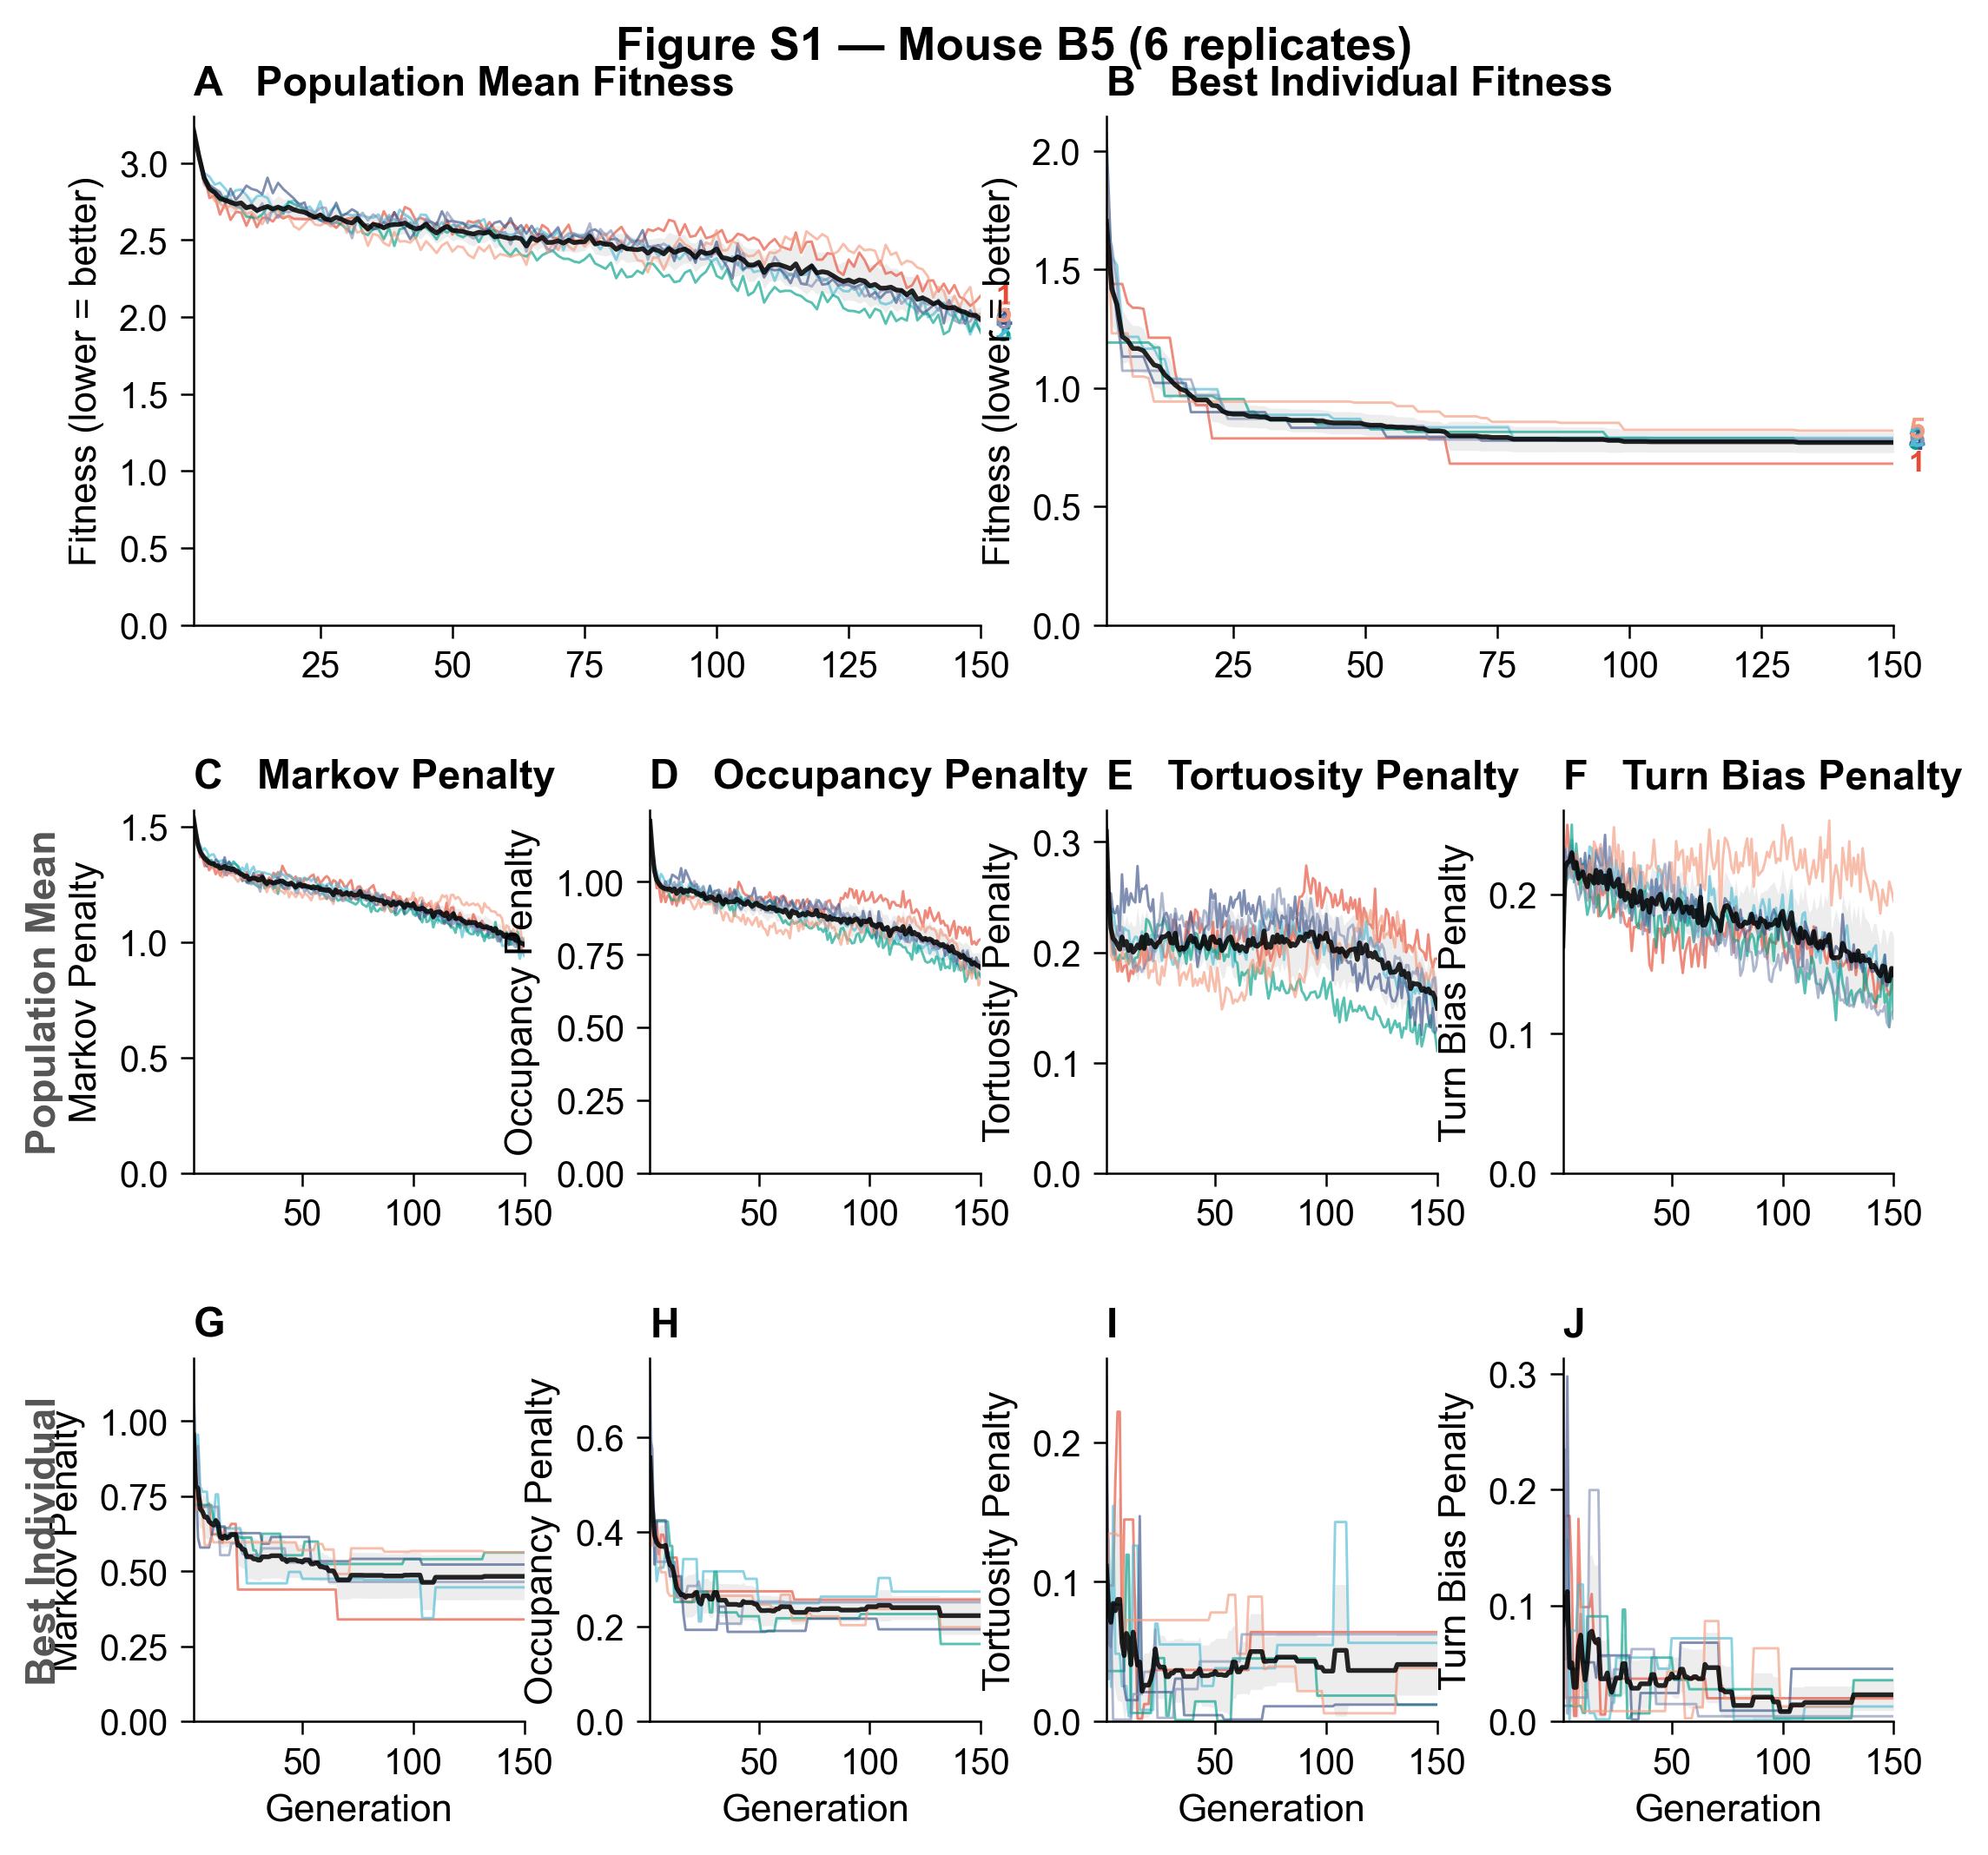
\includegraphics[width=0.45\textwidth]{fig_s1_B5.png}\hfill
  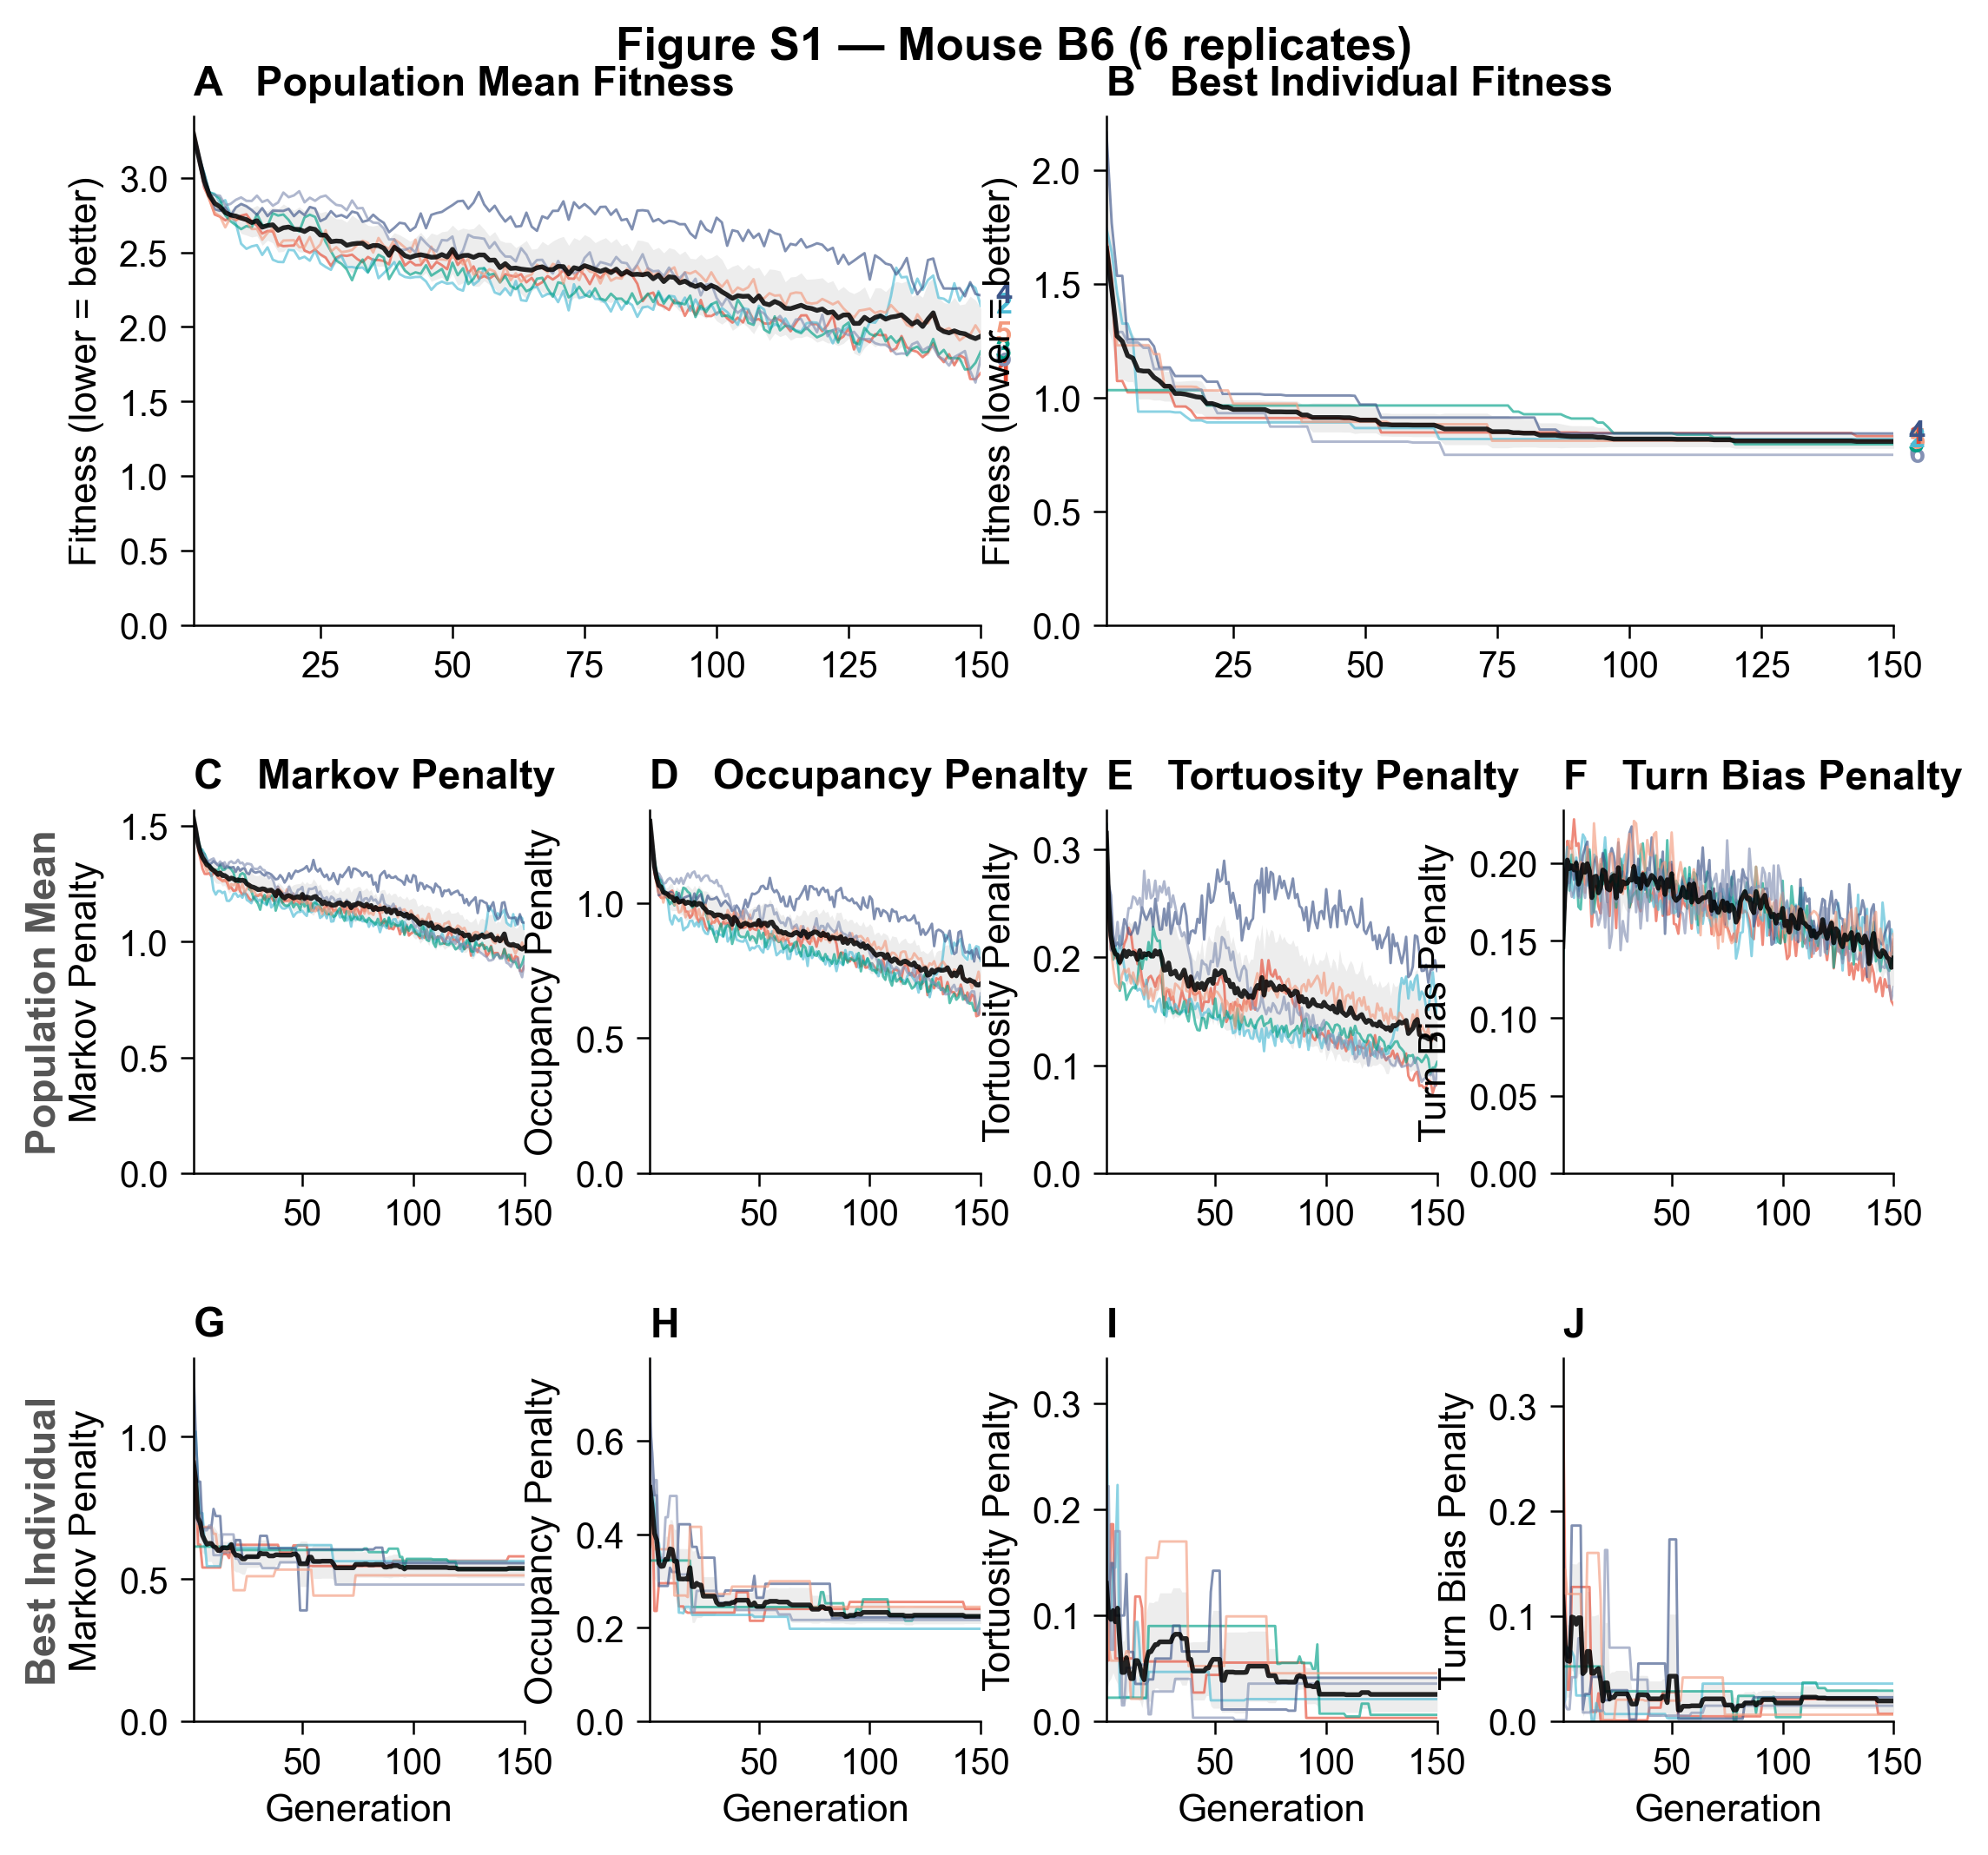
\includegraphics[width=0.45\textwidth]{fig_s1_B6.png}\\[12pt]
  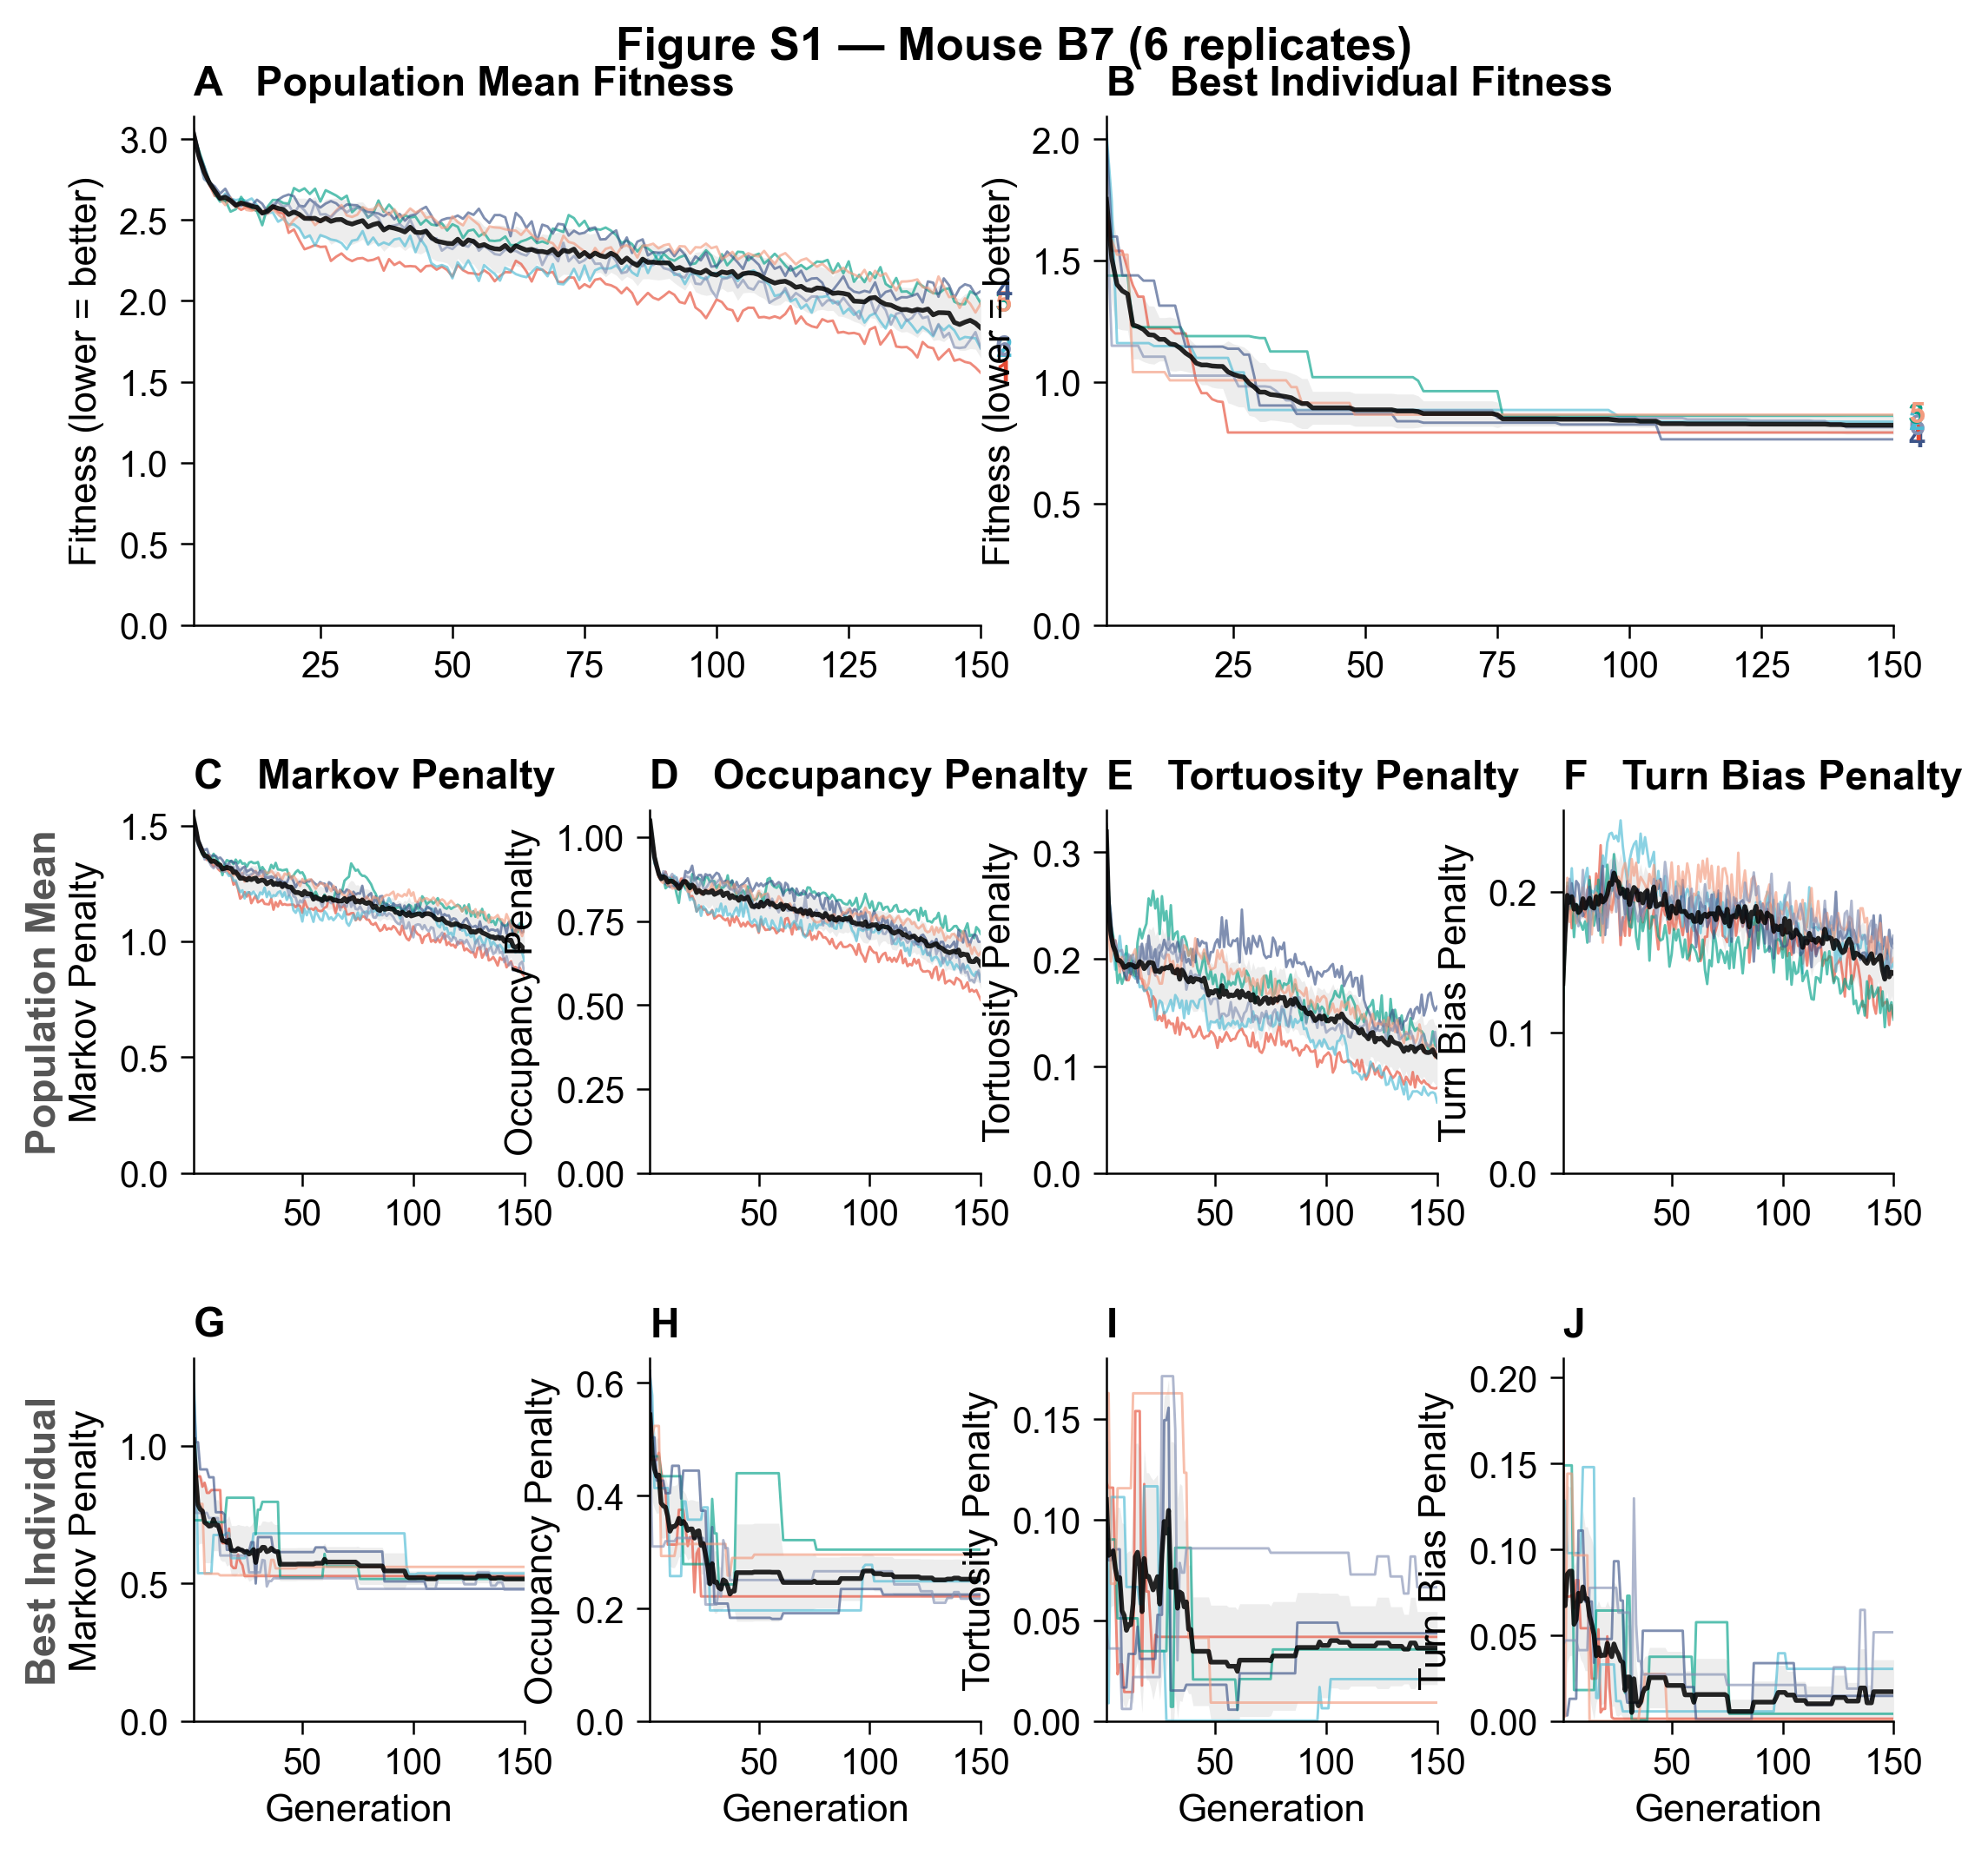
\includegraphics[width=0.45\textwidth]{fig_s1_B7.png}\hfill
  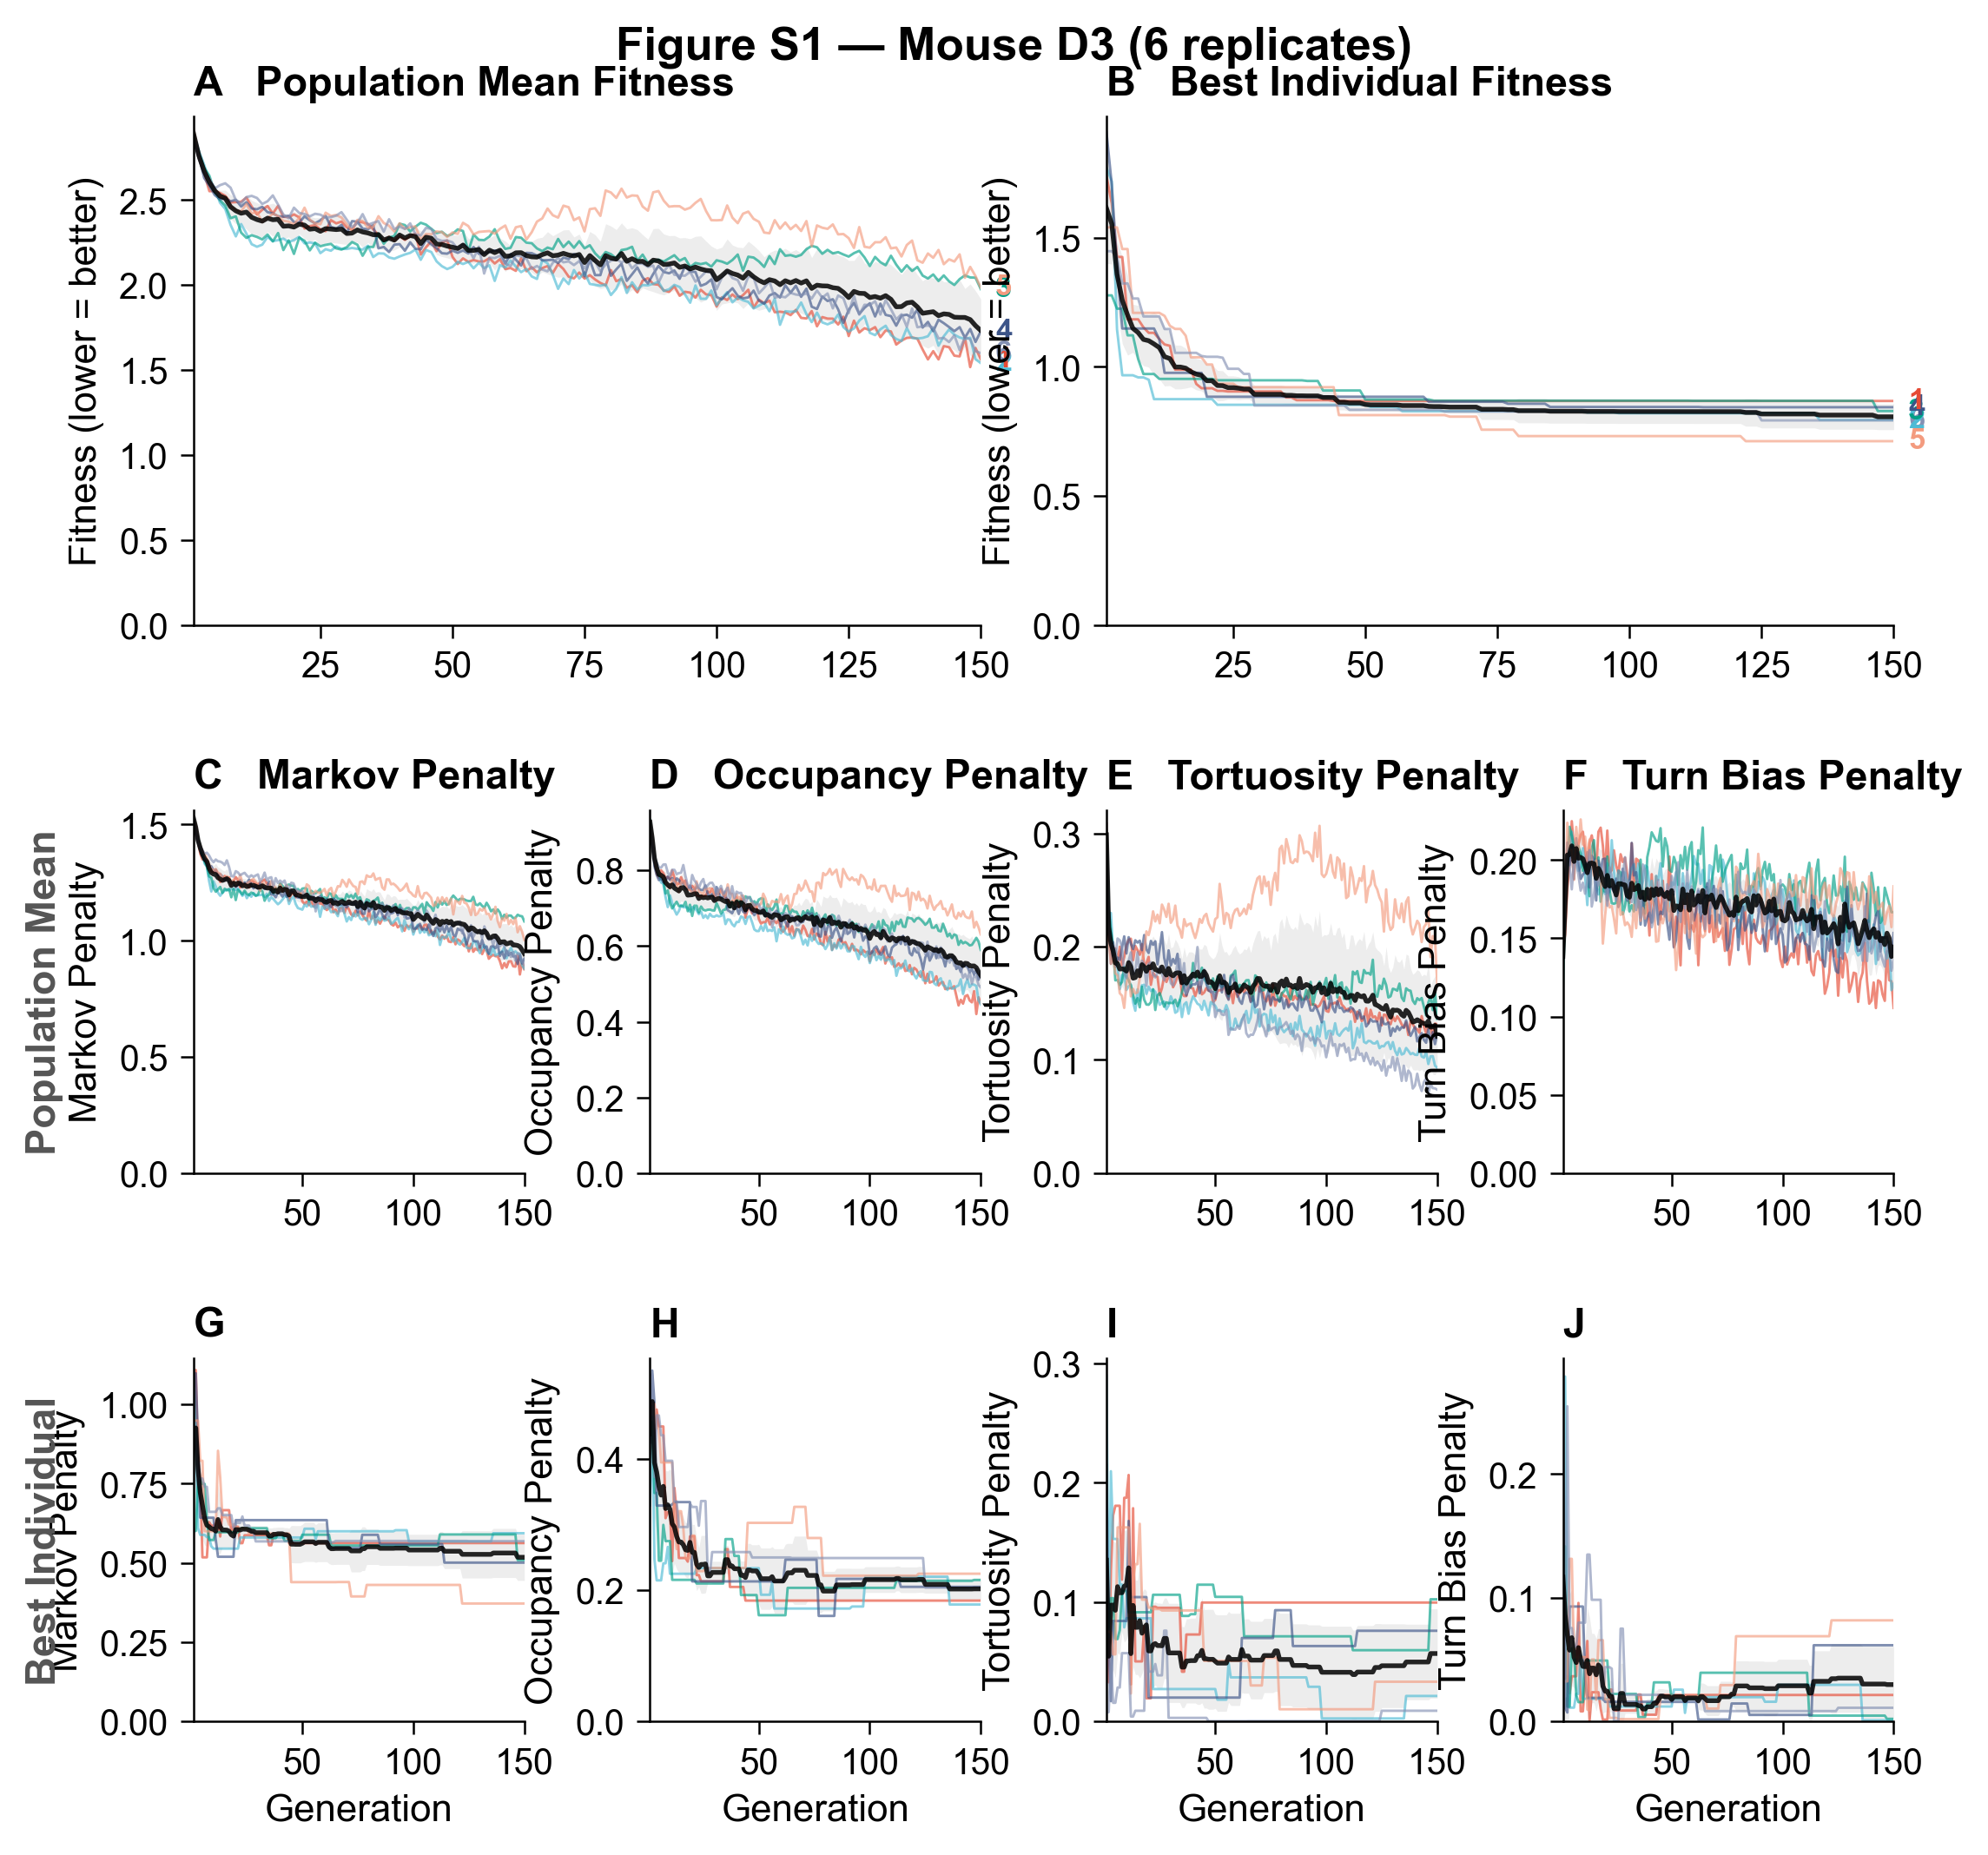
\includegraphics[width=0.45\textwidth]{fig_s1_D3.png}\\[12pt]
  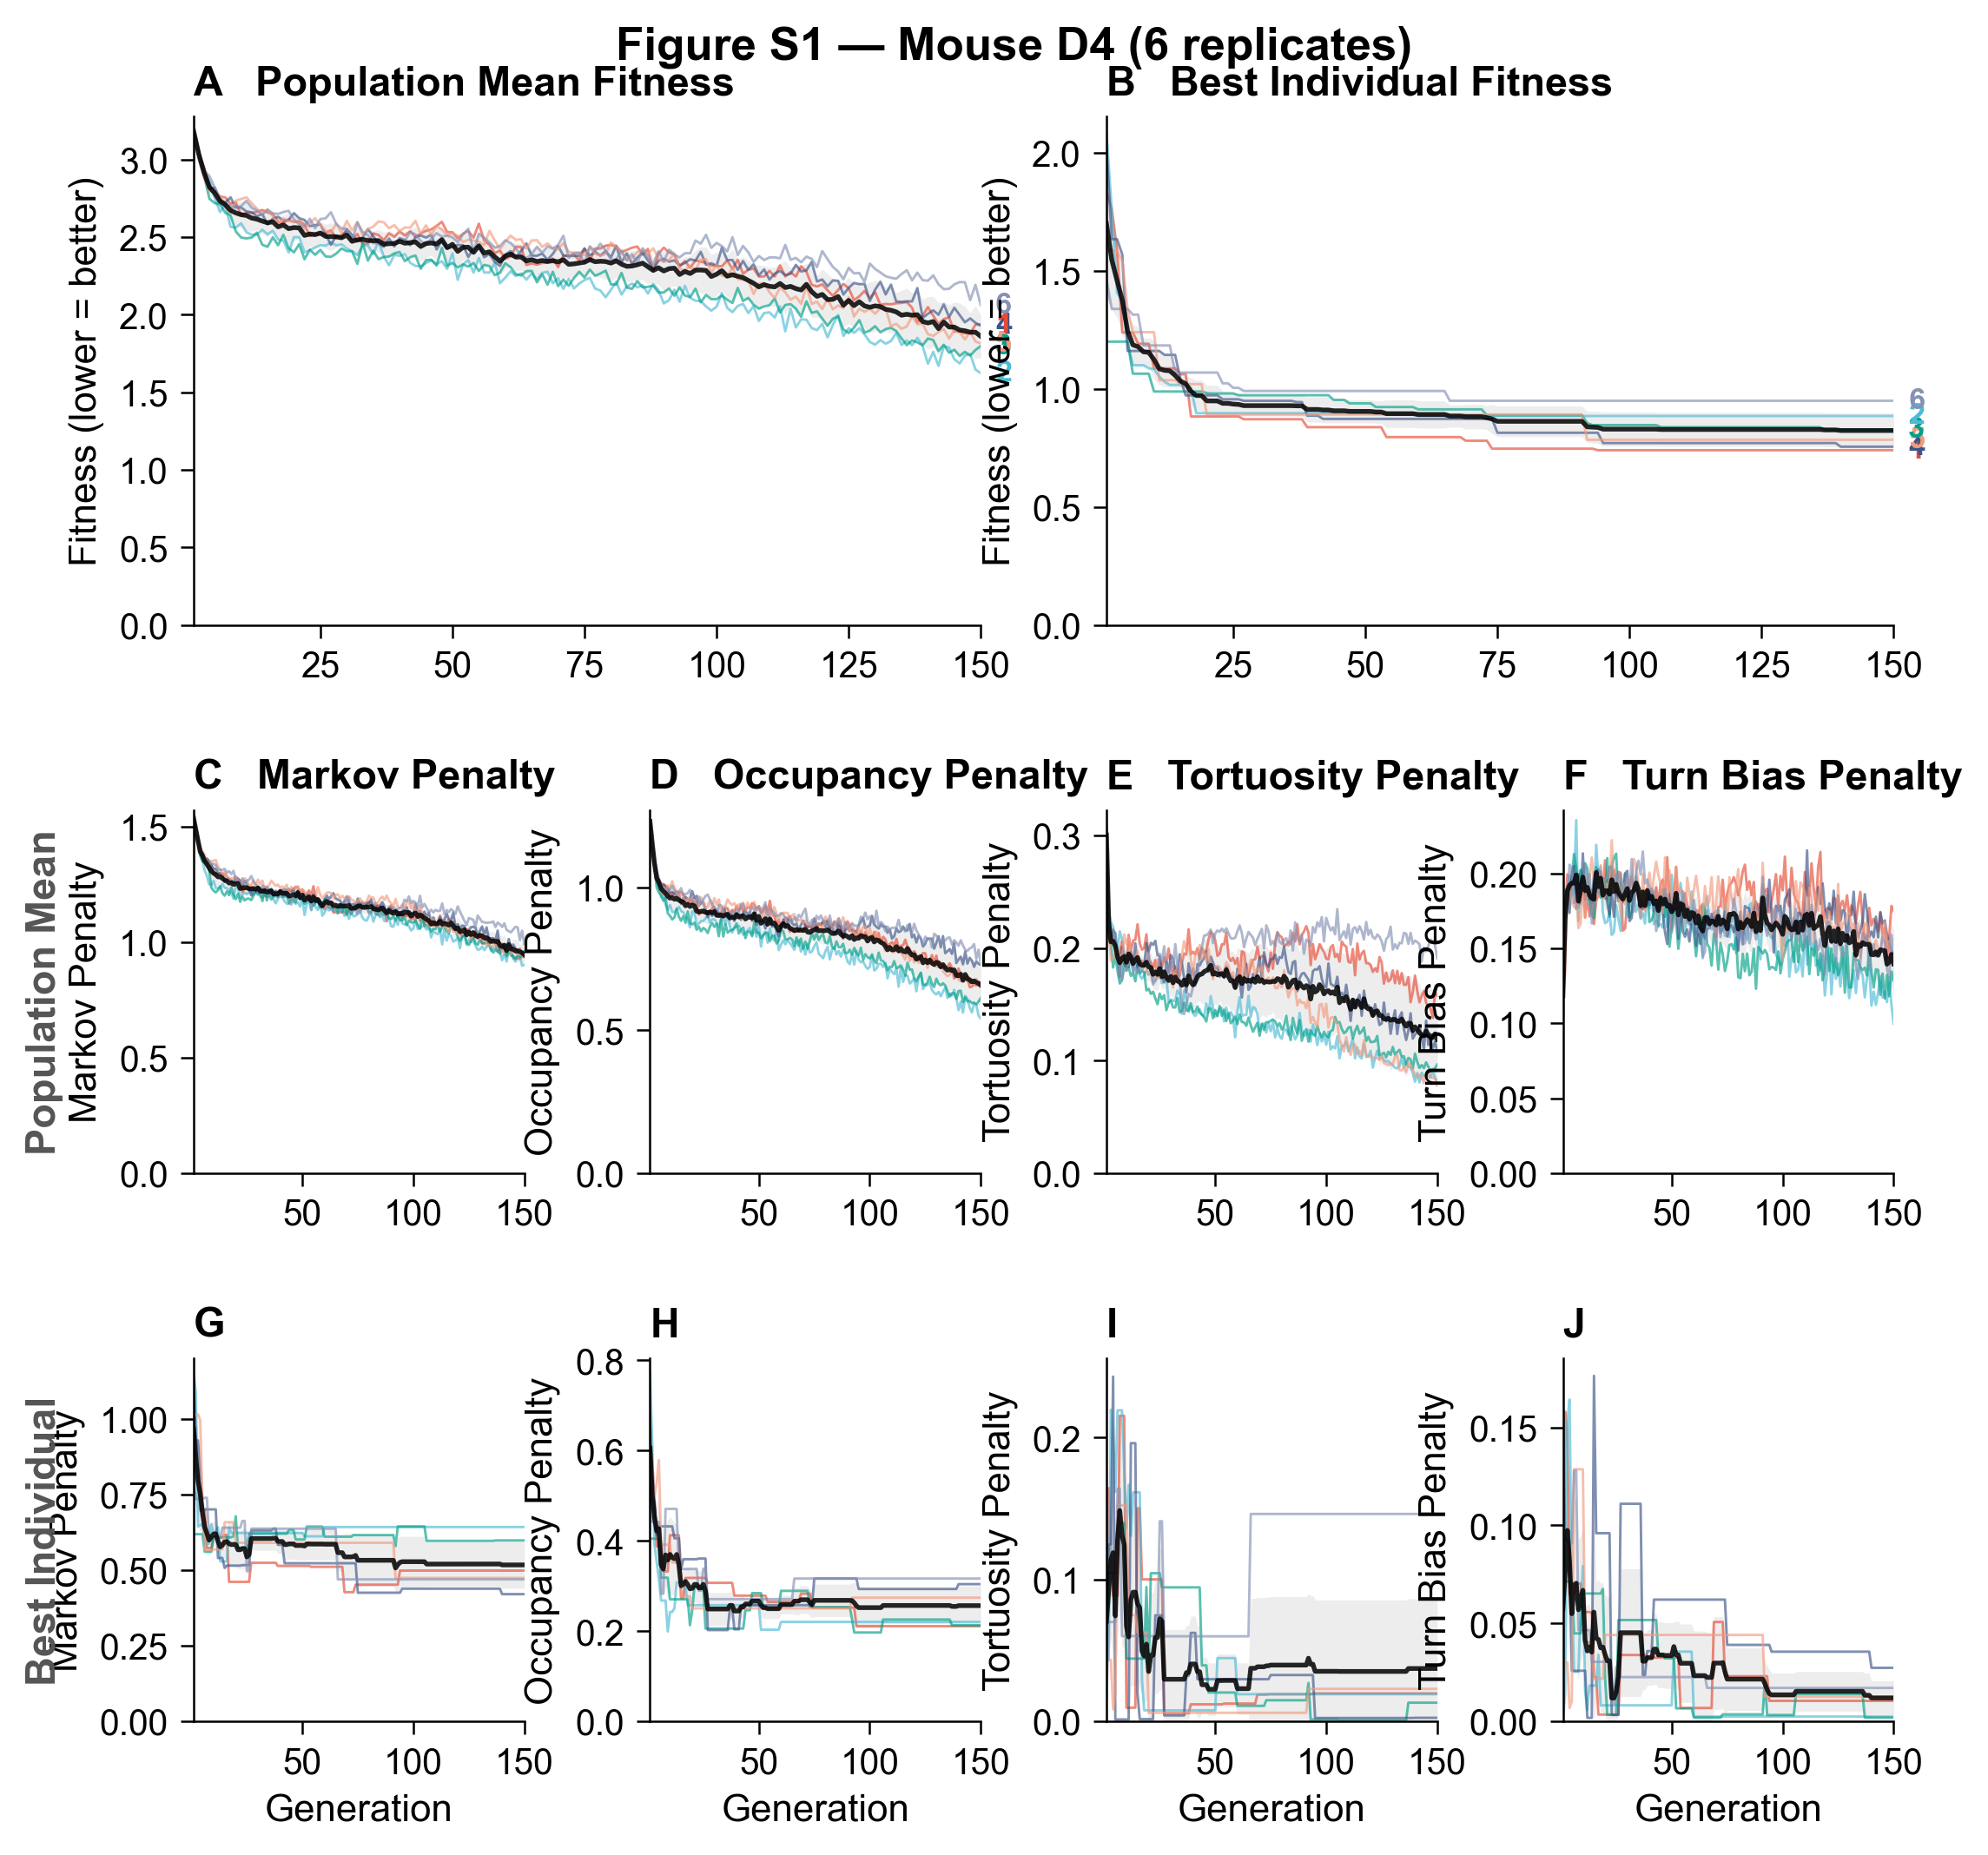
\includegraphics[width=0.45\textwidth]{fig_s1_D4.png}\hfill
  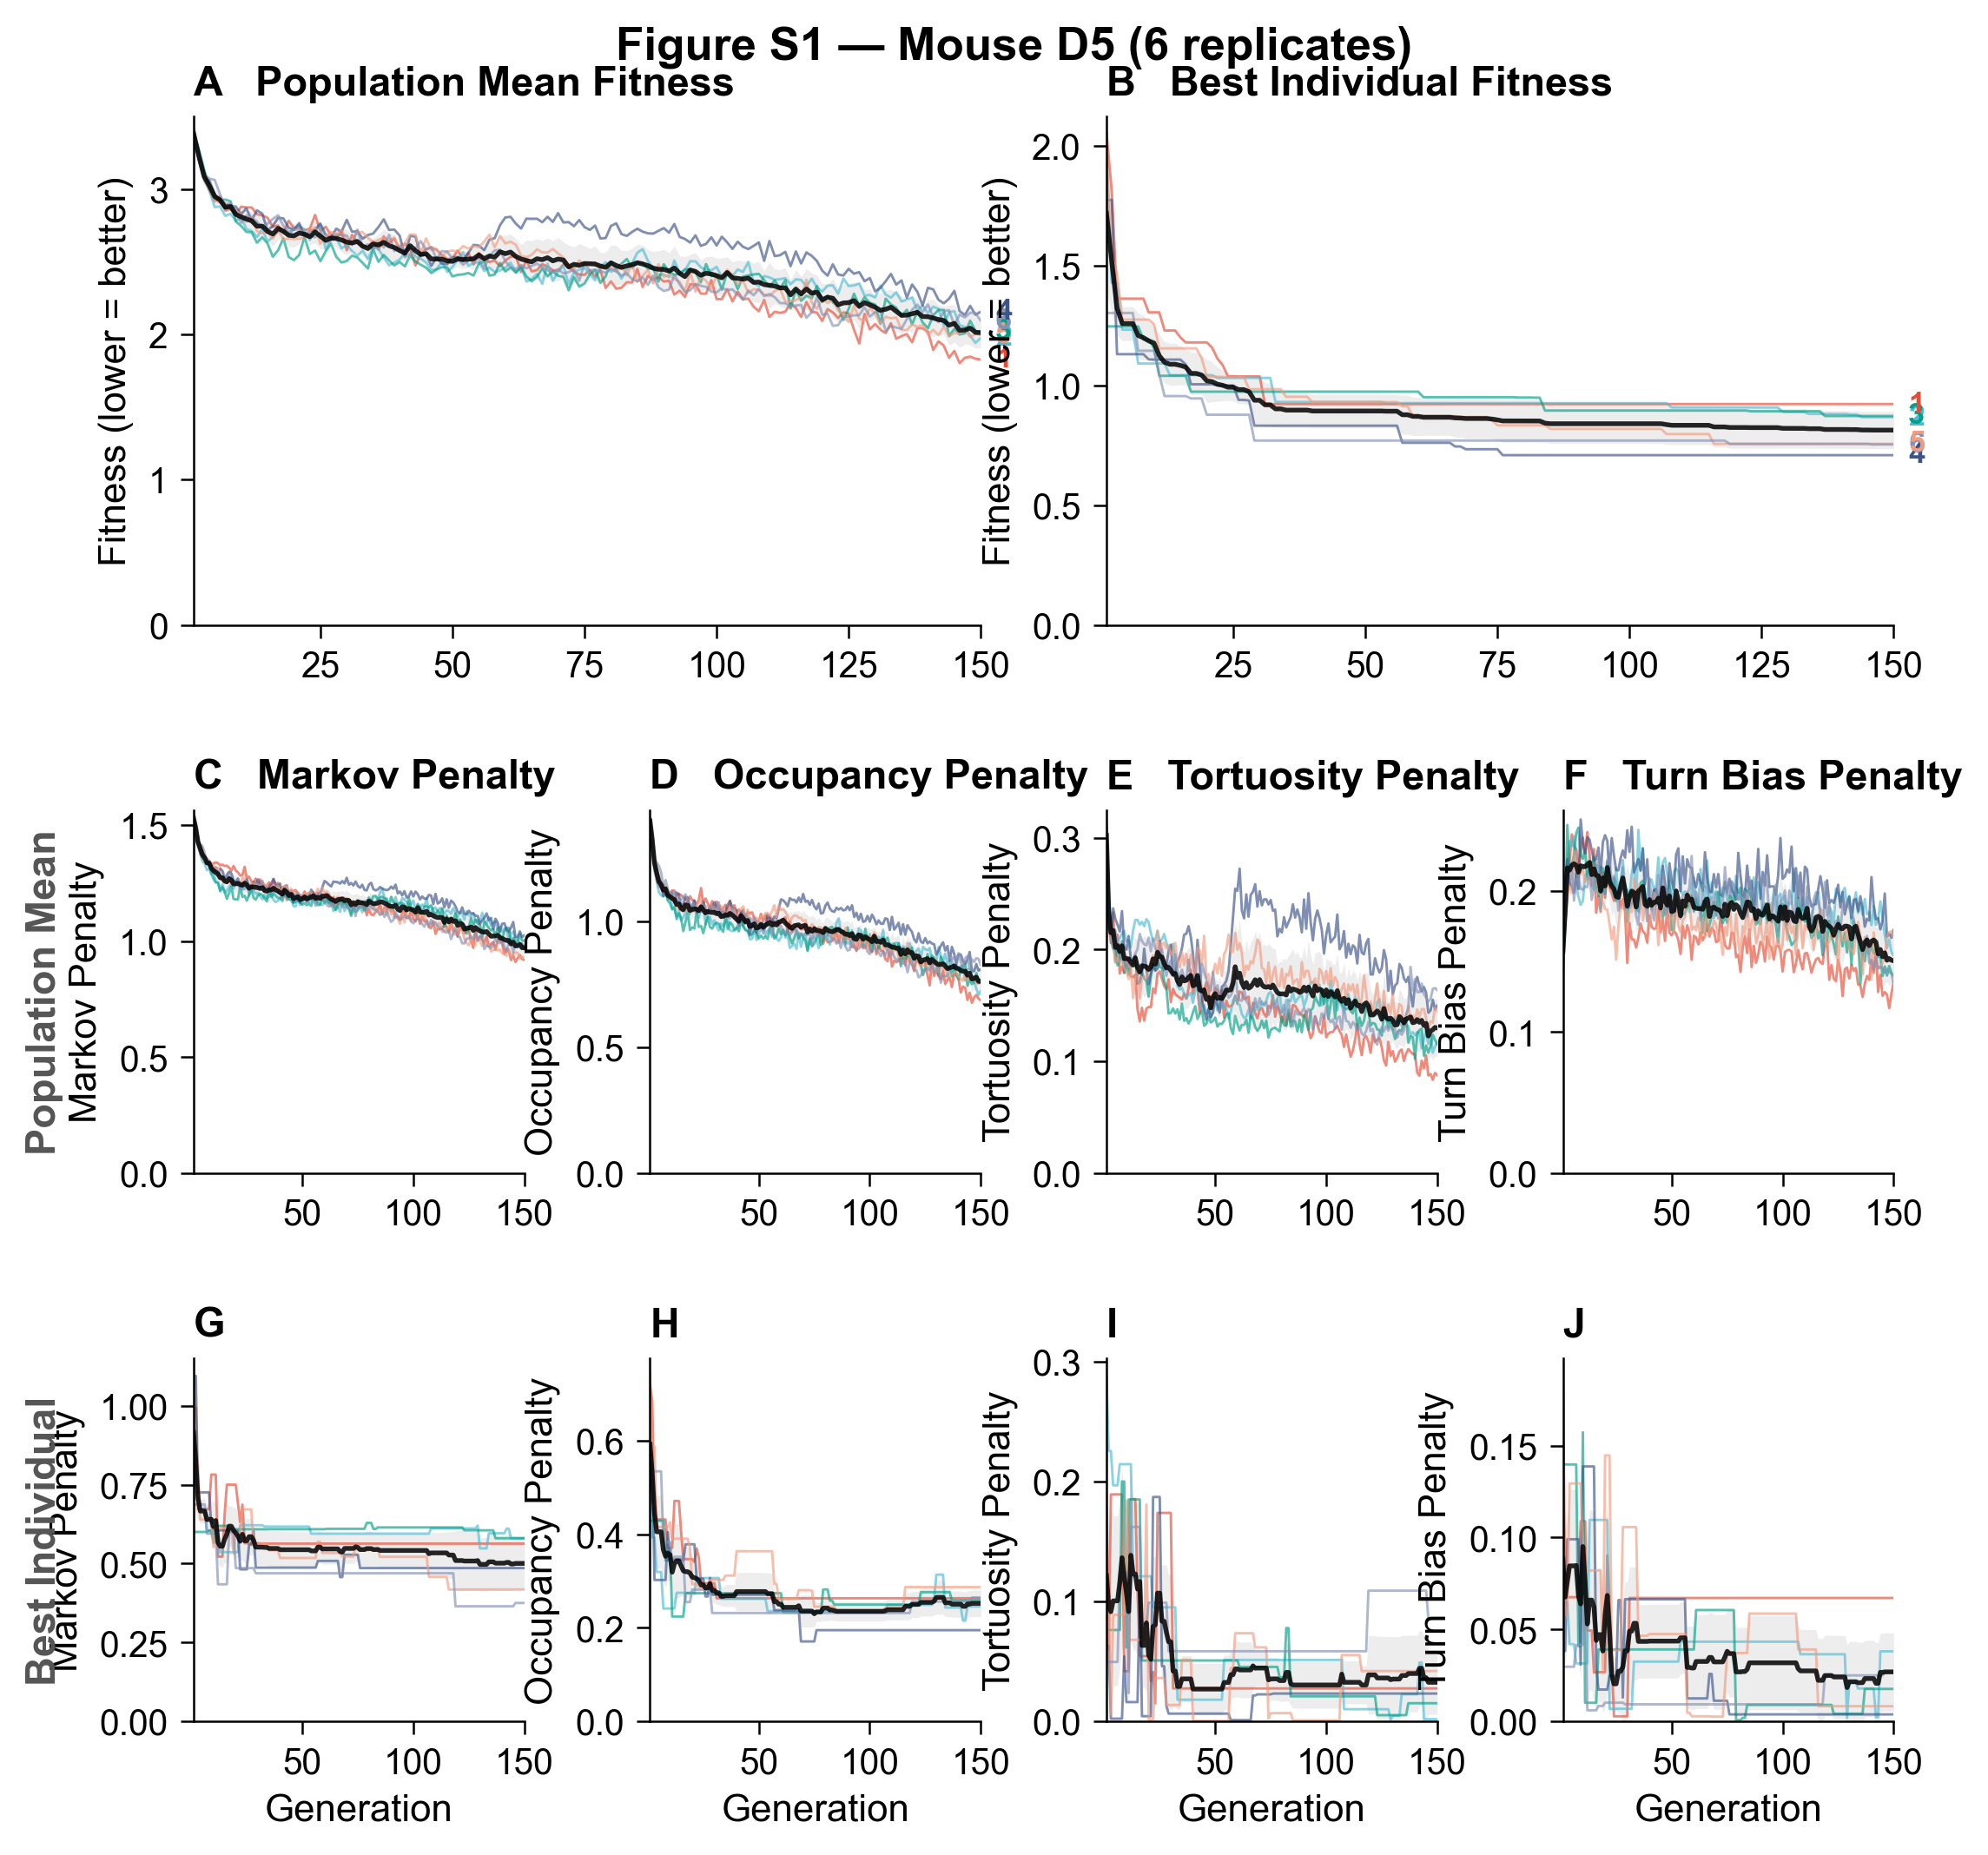
\includegraphics[width=0.45\textwidth]{fig_s1_D5.png}\\[12pt]
  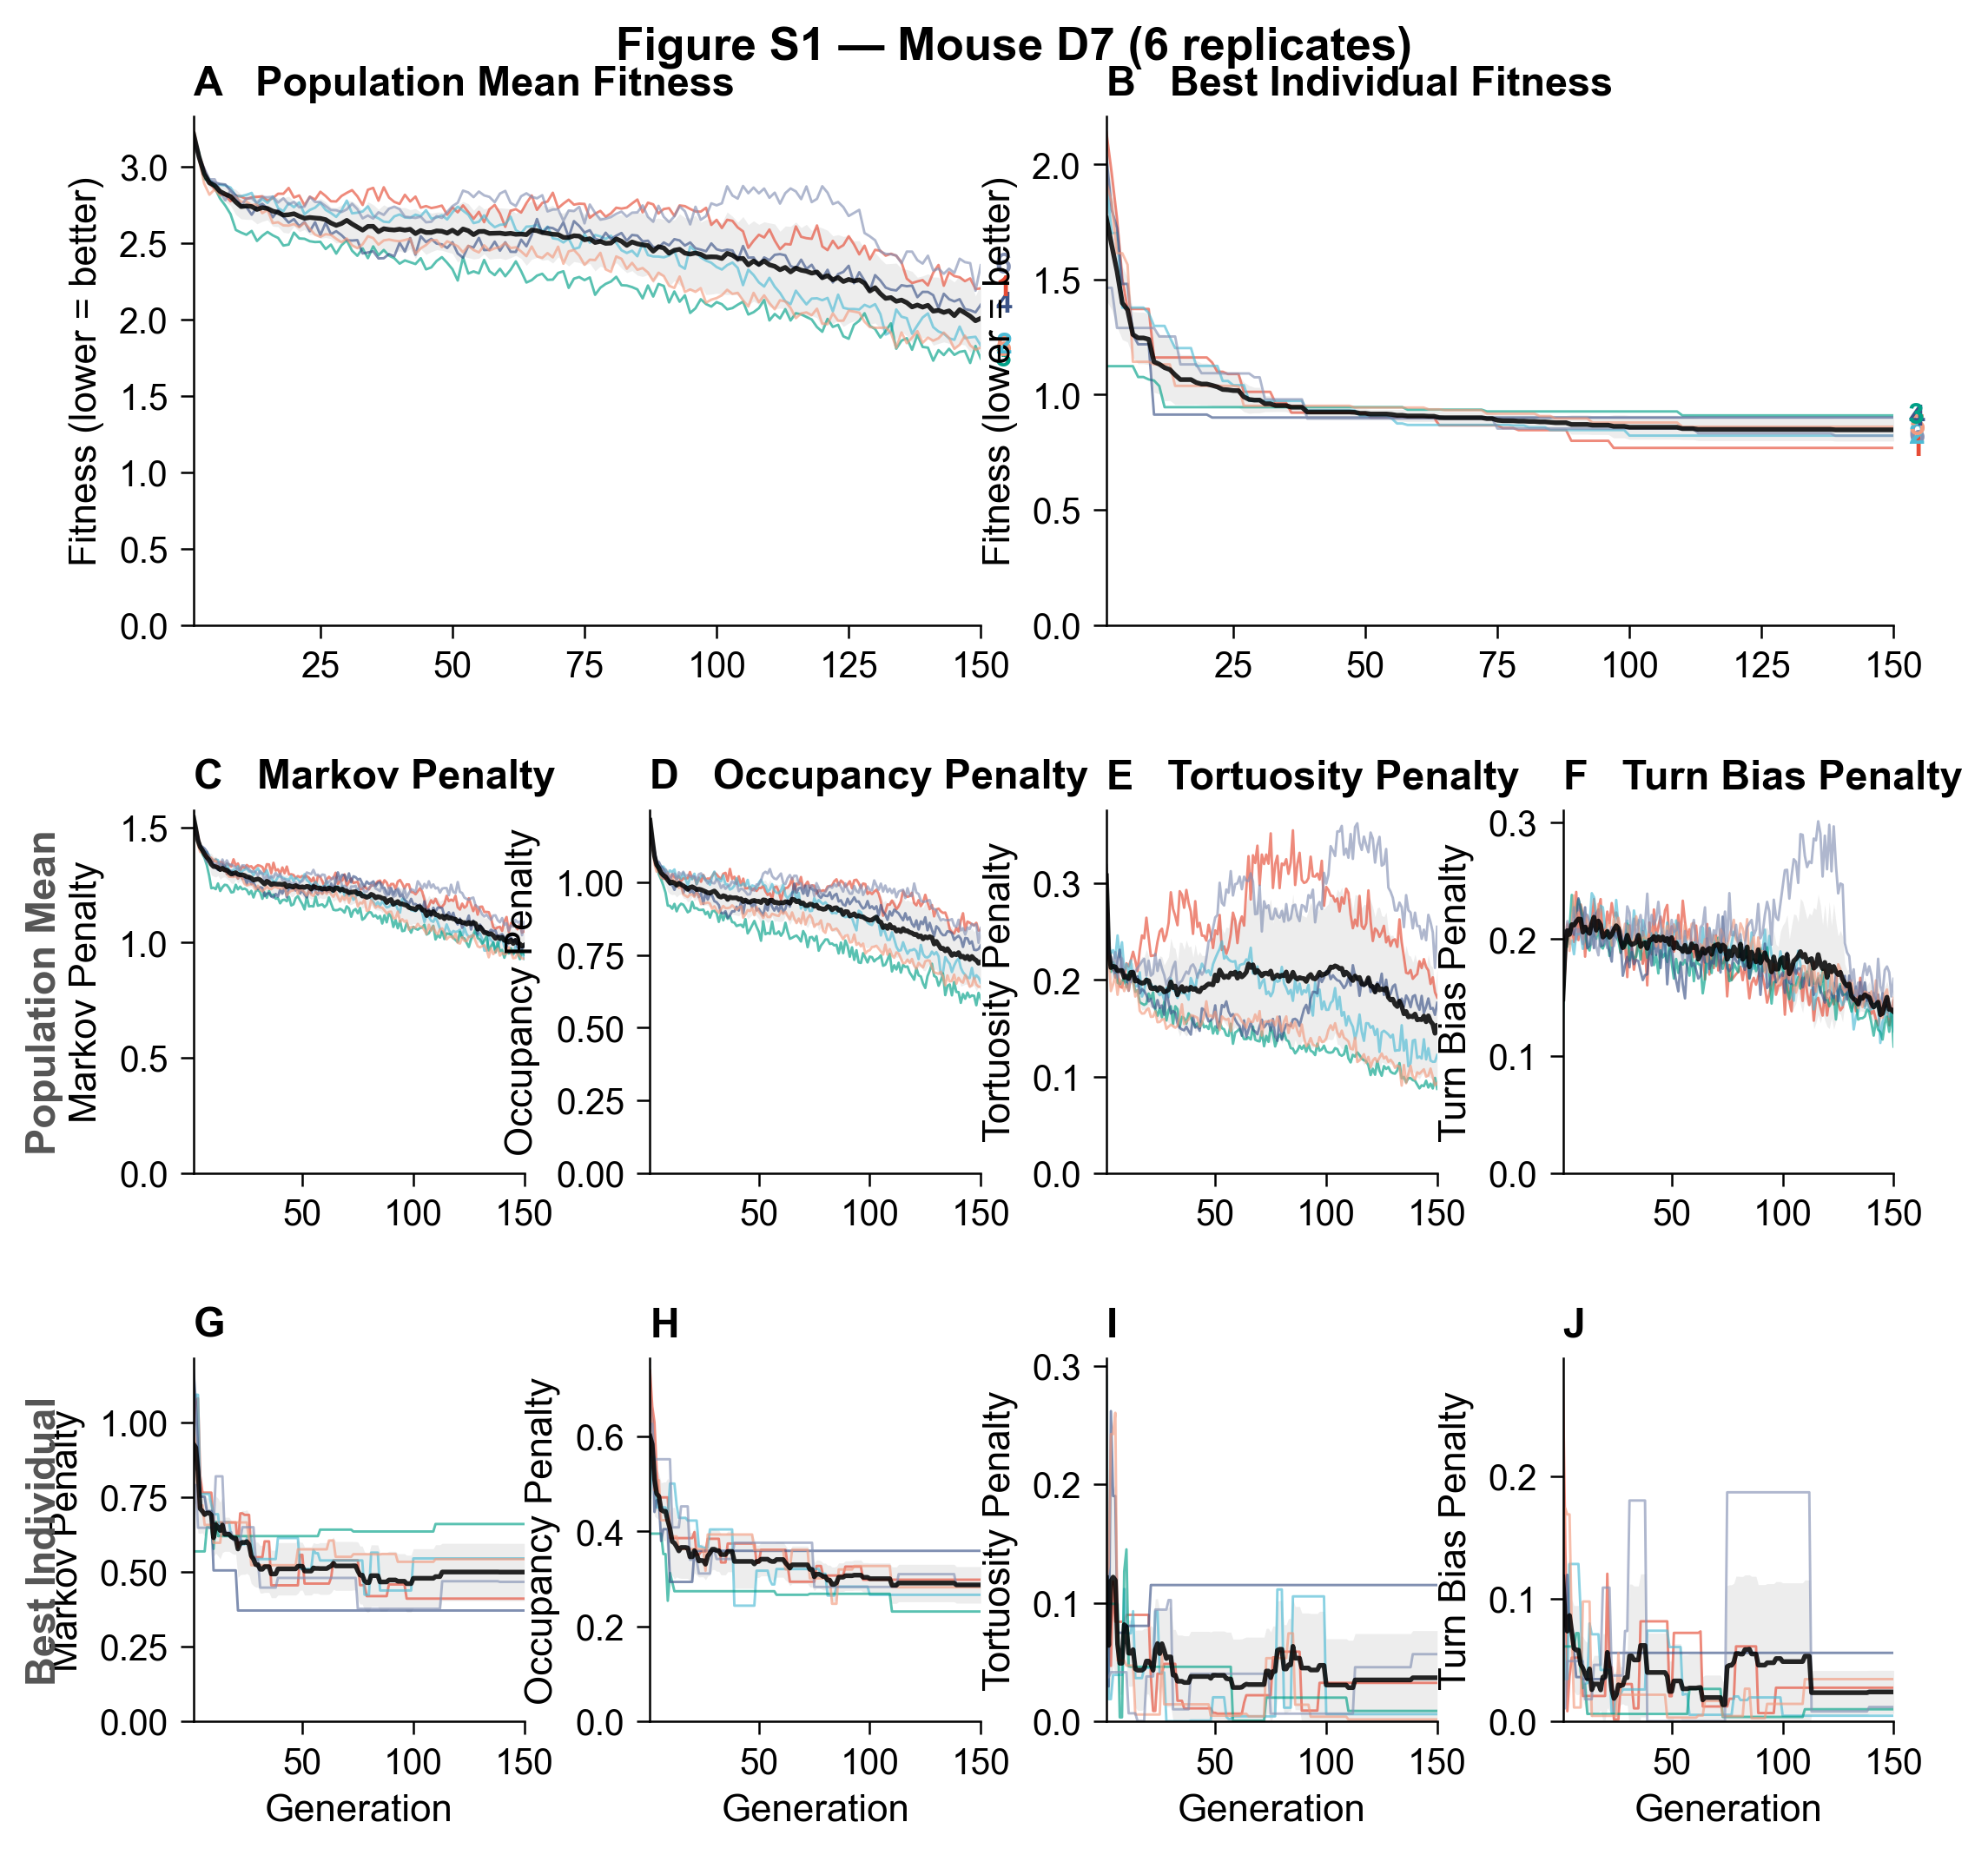
\includegraphics[width=0.45\textwidth]{fig_s1_D7.png}\hfill
  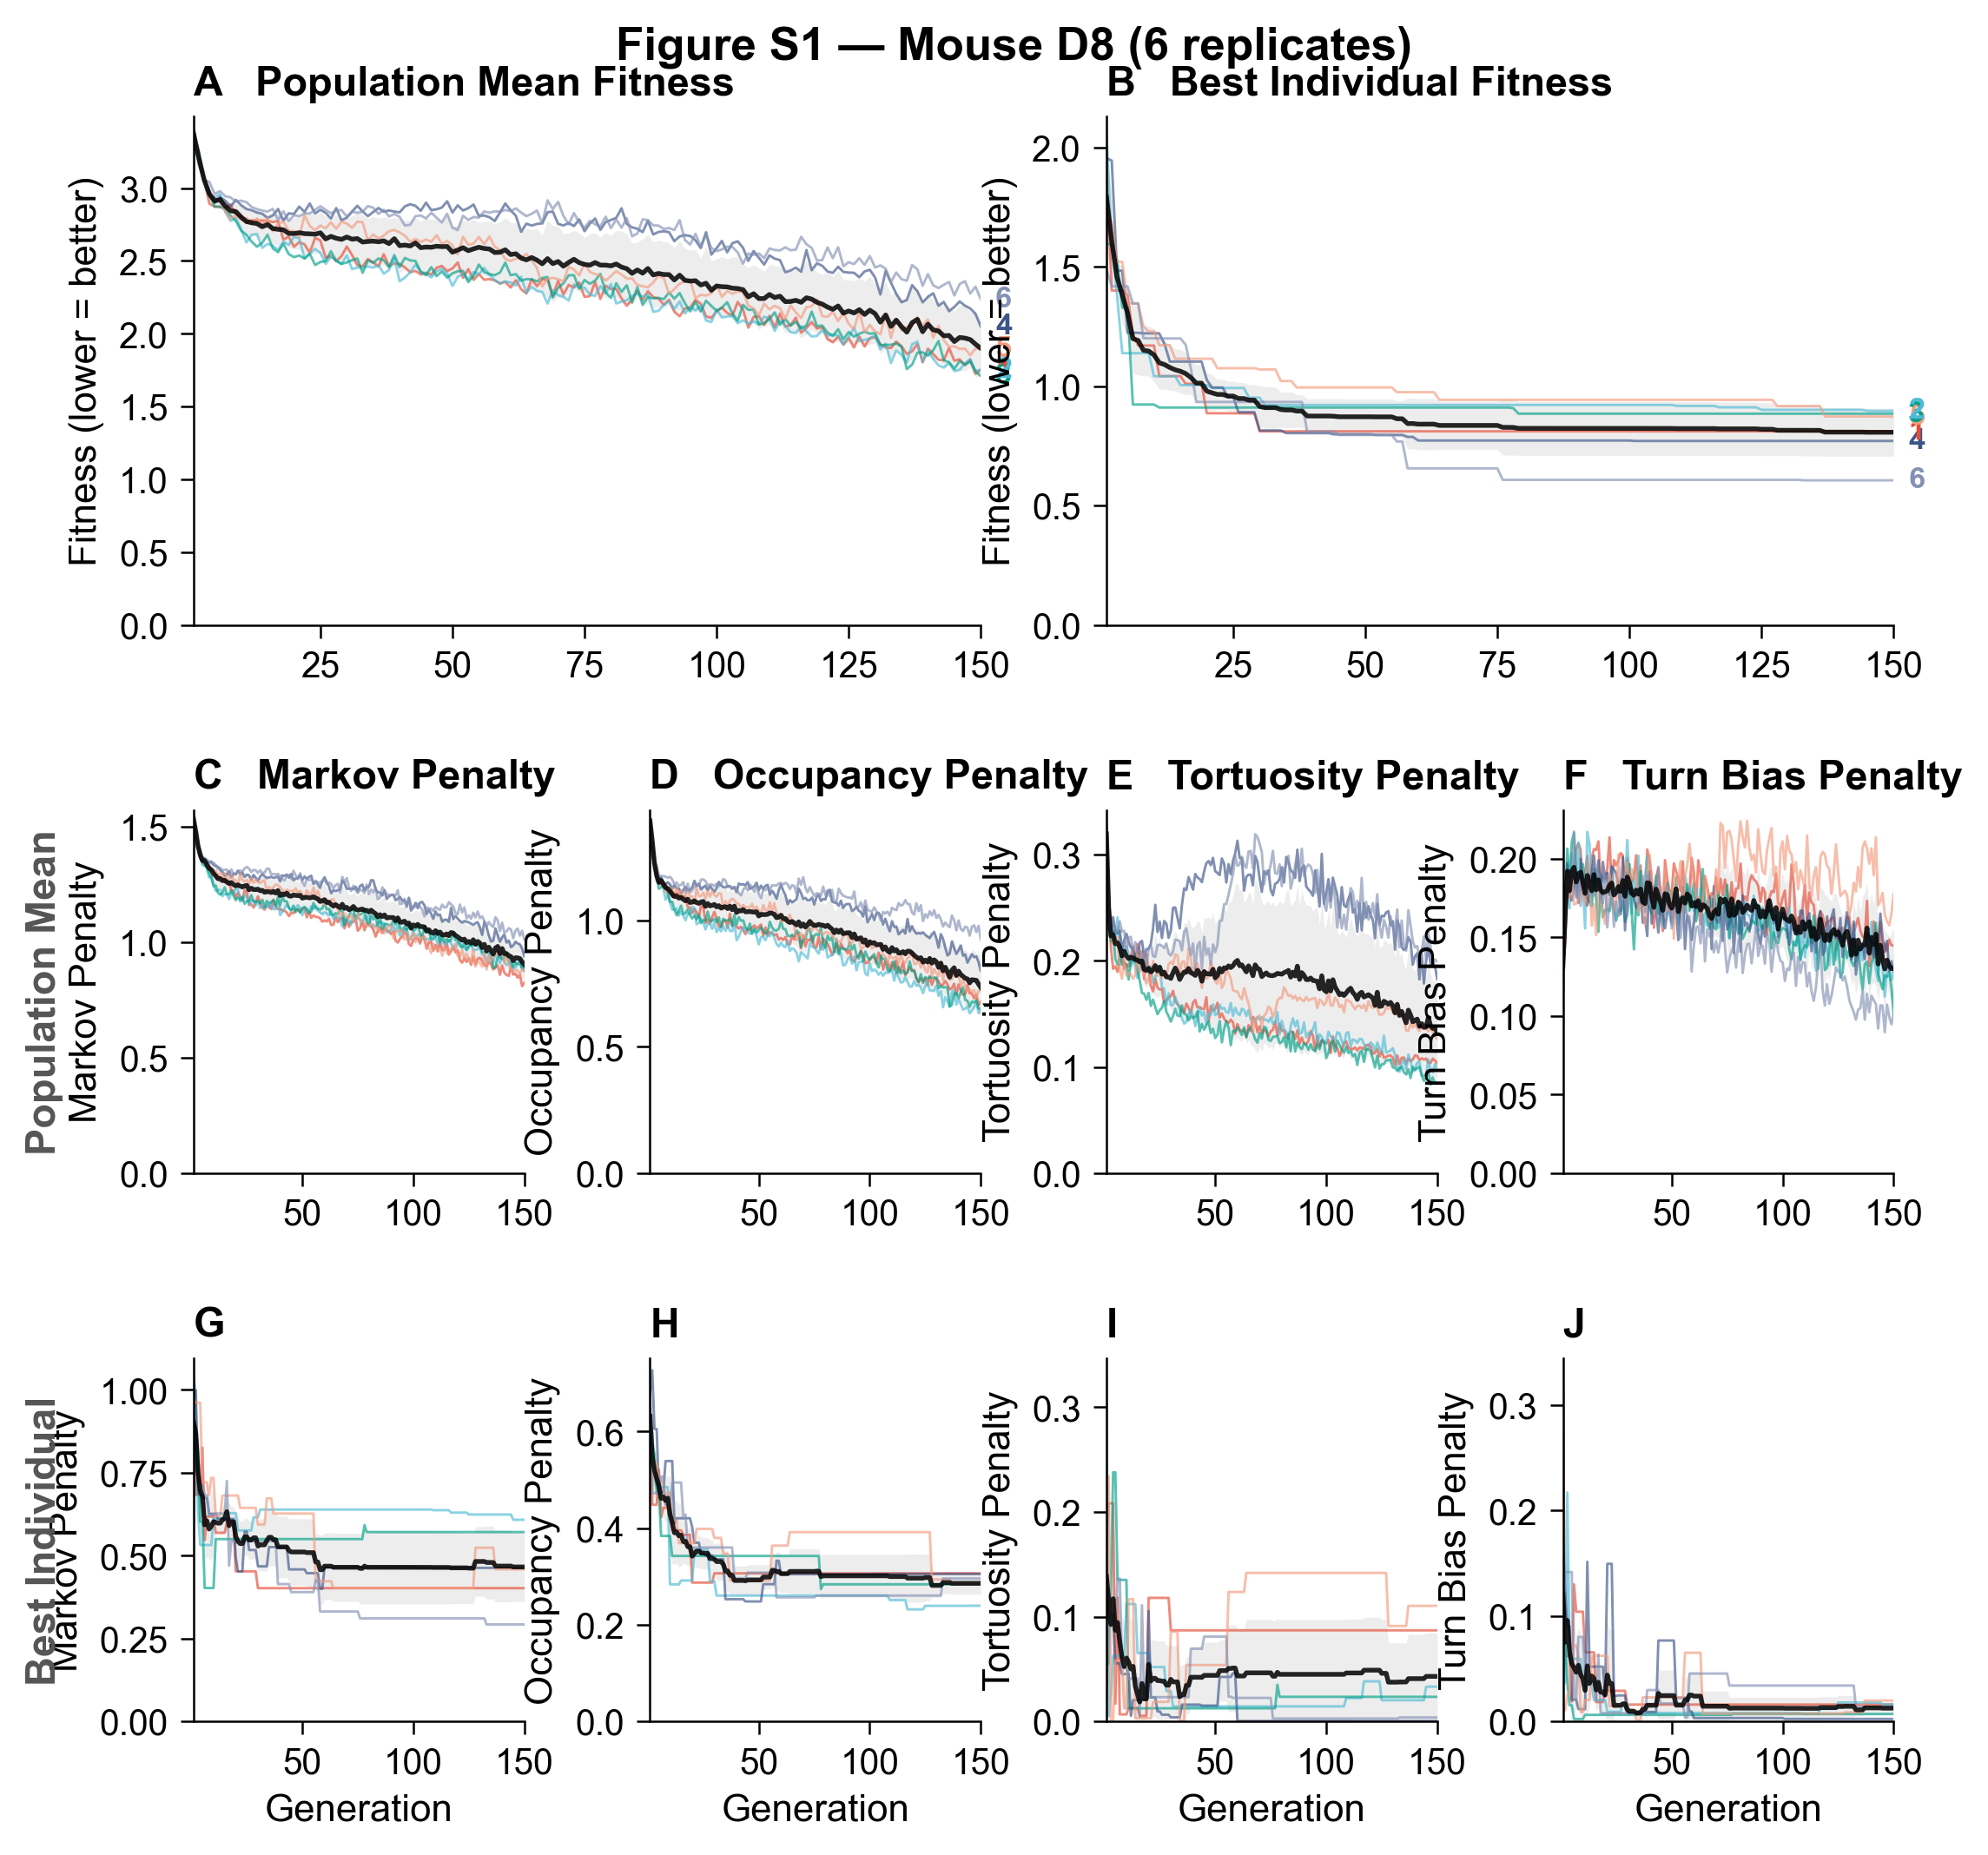
\includegraphics[width=0.45\textwidth]{fig_s1_D8.png}\\[12pt]
  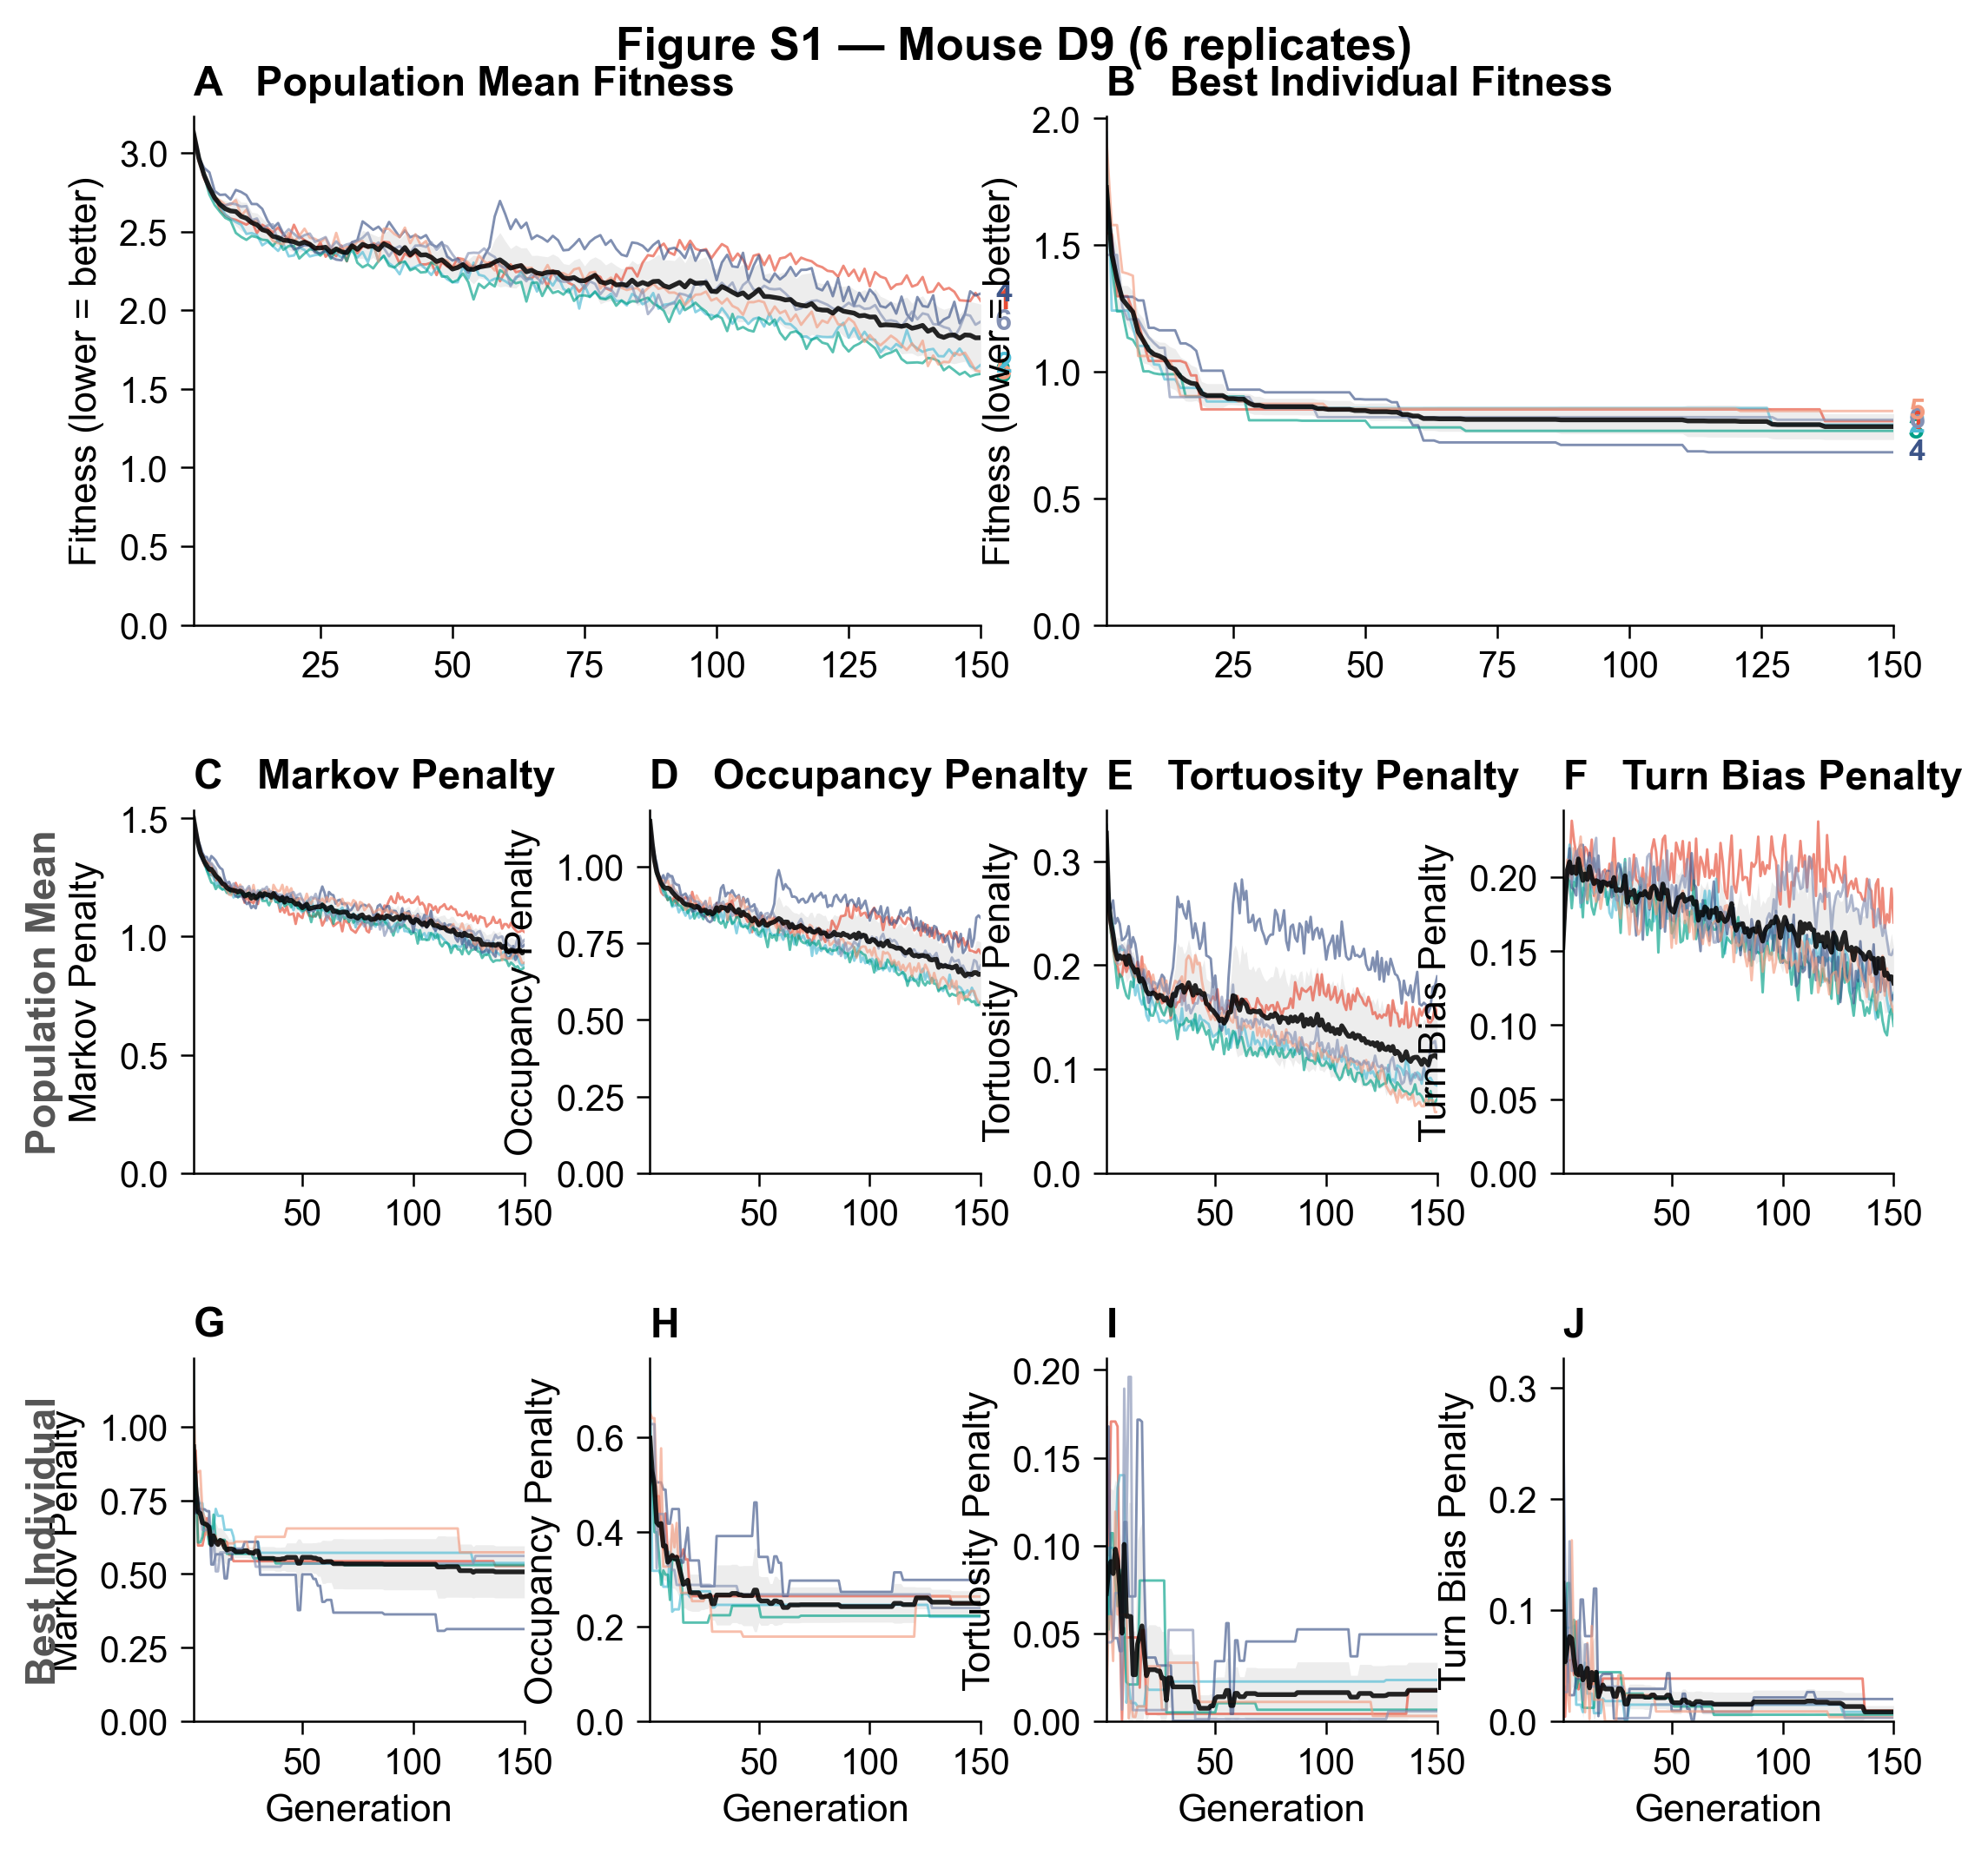
\includegraphics[width=0.45\textwidth]{fig_s1_D9.png}
  \caption{\textbf{Per-mouse individual replicate trajectories.}
  Population mean fitness (solid lines) and best-of-generation fitness (dashed lines)
  across 150 generations. Lower fitness = better behavioral match to the target mouse.}
  \label{fig:supp_per_mouse_individual}
\end{figure}

% ----------------------------------------------------------------------------
\subsection*{S2. Evolved network diagrams per mouse}
\label{sec:supp_networks_per_mouse}

Representative best-evolved network diagram for each of the 9 mice. Excitatory
connections are shown in red, inhibitory in blue; connection width encodes weight
magnitude. Despite identical aggregate structural statistics, the specific
who-connects-to-whom topology varies across mice and replicates.

\begin{figure}[H]
  \centering
  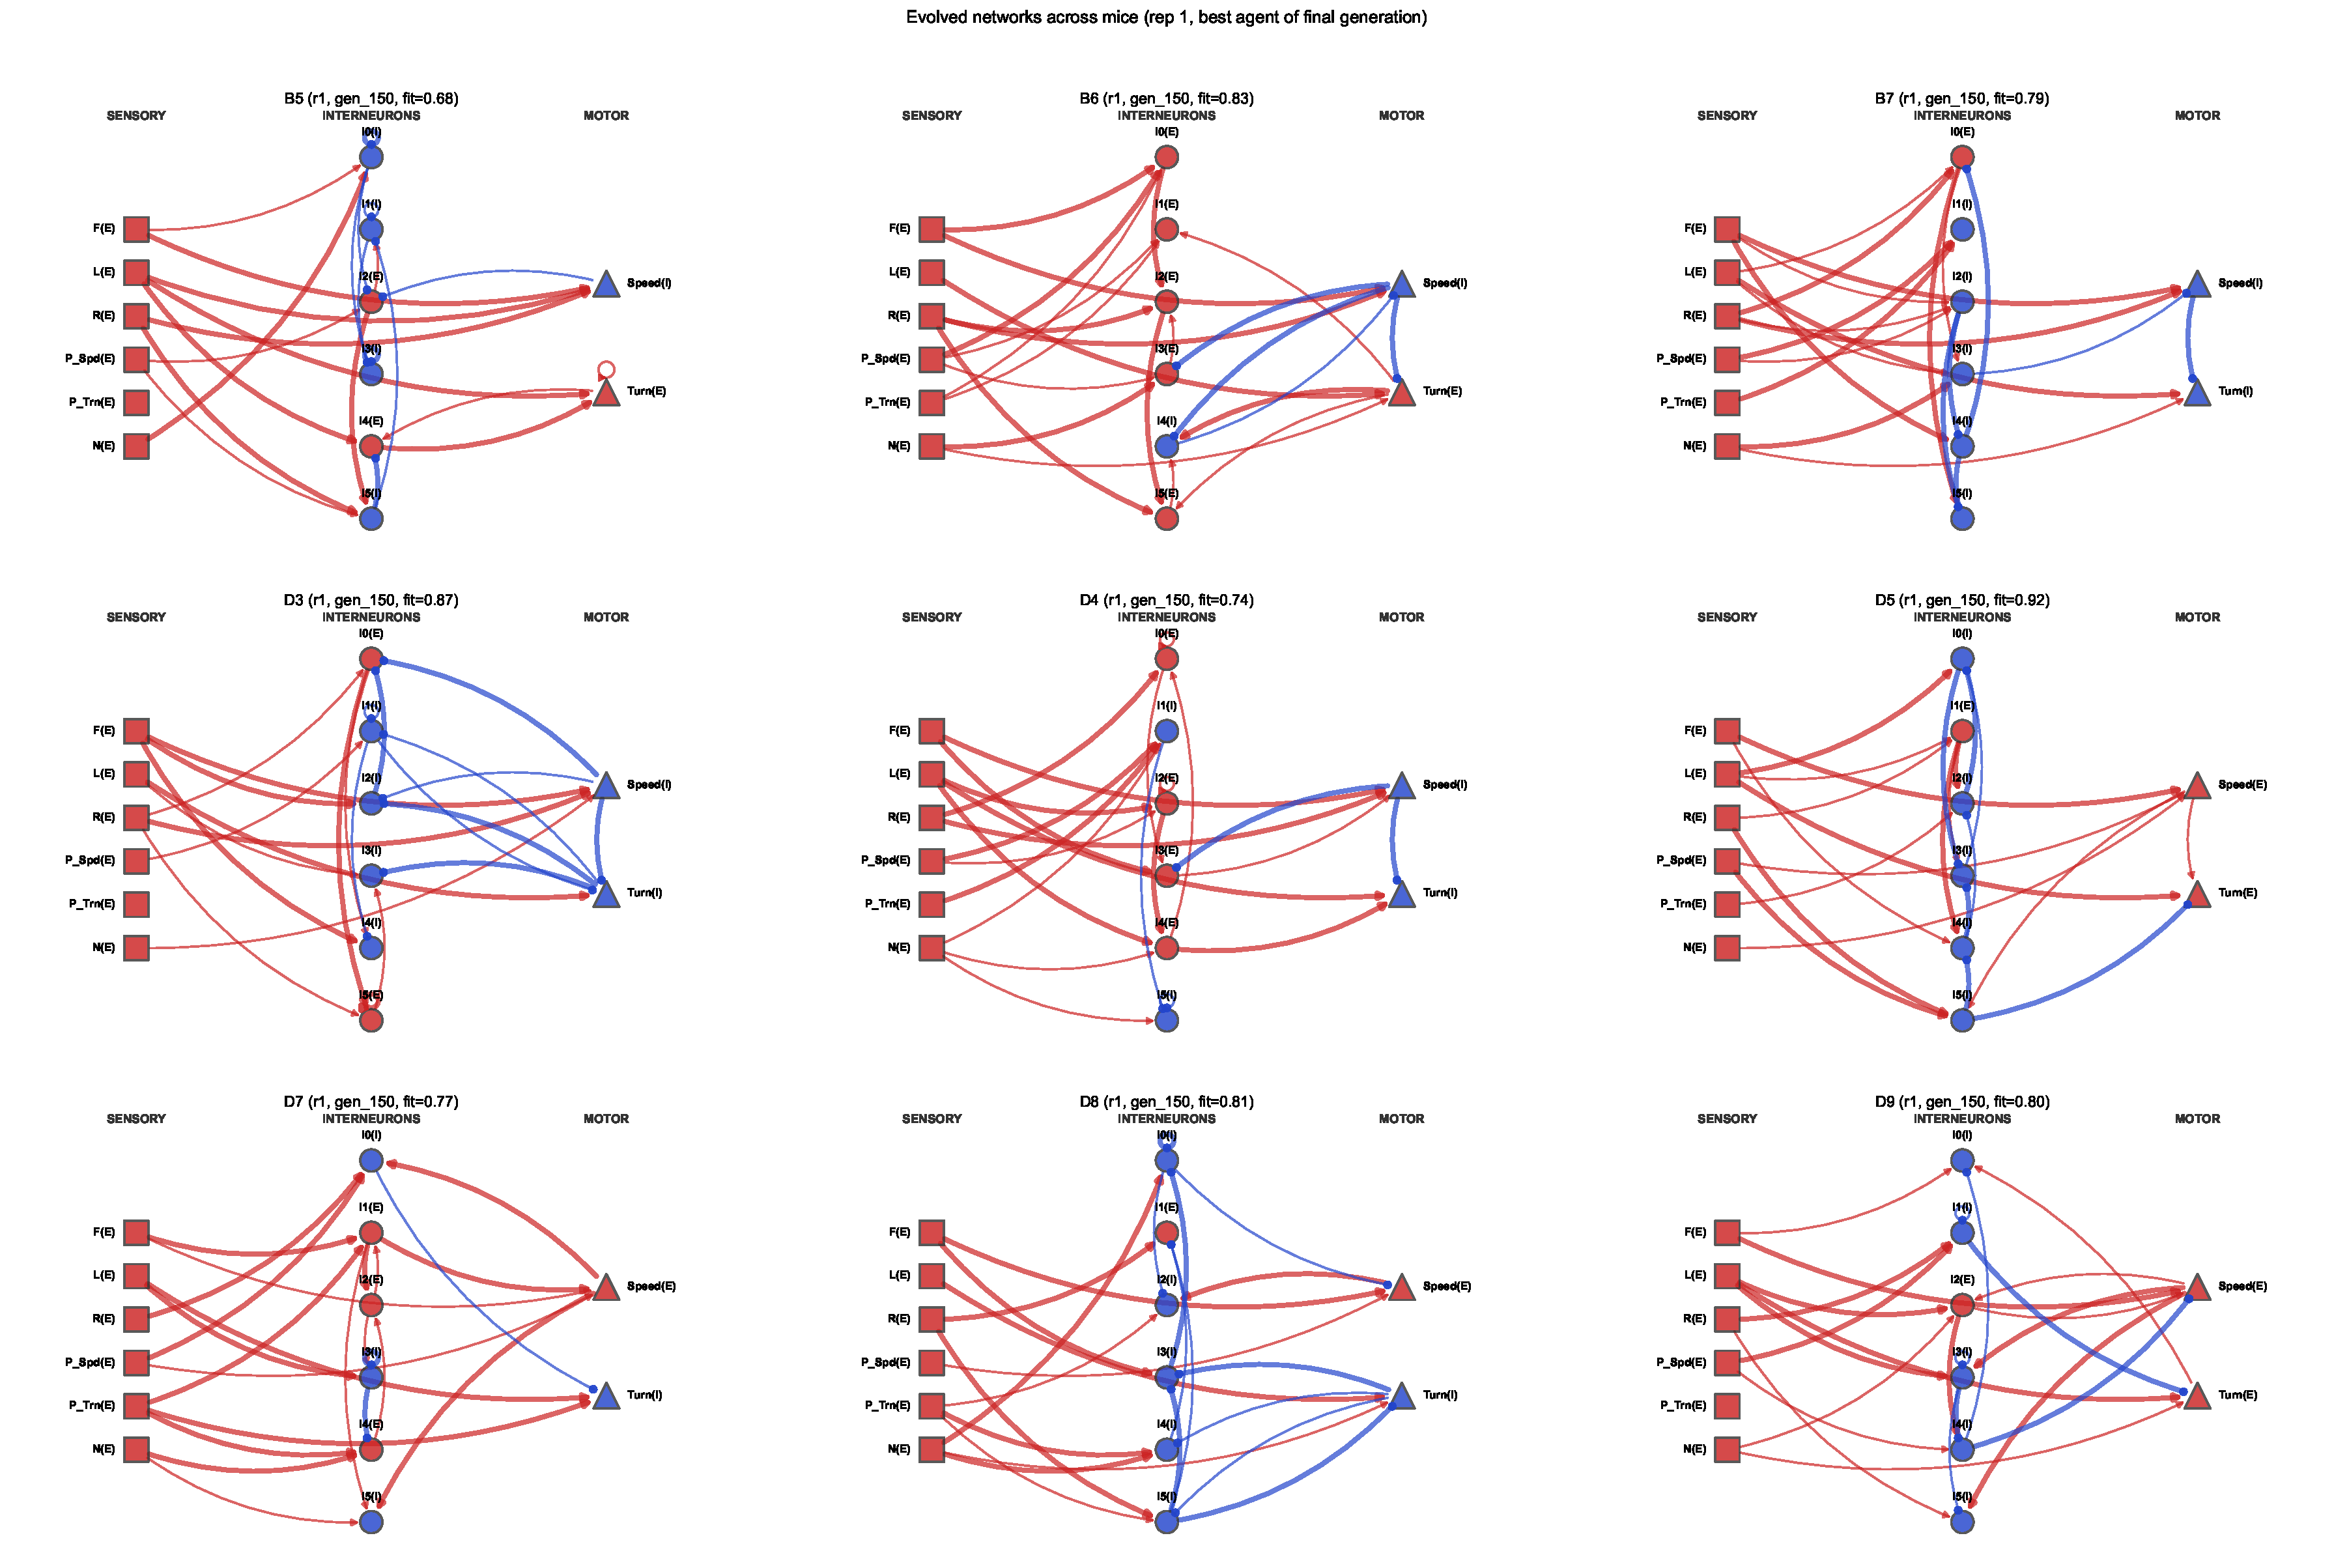
\includegraphics[width=\textwidth]{fig_supp_networks_per_mouse.pdf}
  \caption{\textbf{Evolved network diagrams for all 9 mice.}
  Best-evolved agent per mouse at generation 150. Node types: squares = sensory,
  circles = interneuron, triangles = motor. Red = excitatory, blue = inhibitory;
  line width $\propto$ weight magnitude.}
  \label{fig:supp_networks_per_mouse}
\end{figure}

% ----------------------------------------------------------------------------
\subsection*{S3. Per-metric convergence curves}
\label{sec:supp_convergence_permouse}

Figure~\ref{fig:supp_convergence_permouse} shows the evolutionary convergence
broken down by the four fitness components, with population mean and
best-of-generation curves per mouse. KDE insets (panels C--F) show the
distribution of generation-150 fitness values across replicates for each mouse.
The Markov and occupancy components (weighted 2$\times$) account for most
early-generation improvement.

\begin{figure}[H]
  \centering
  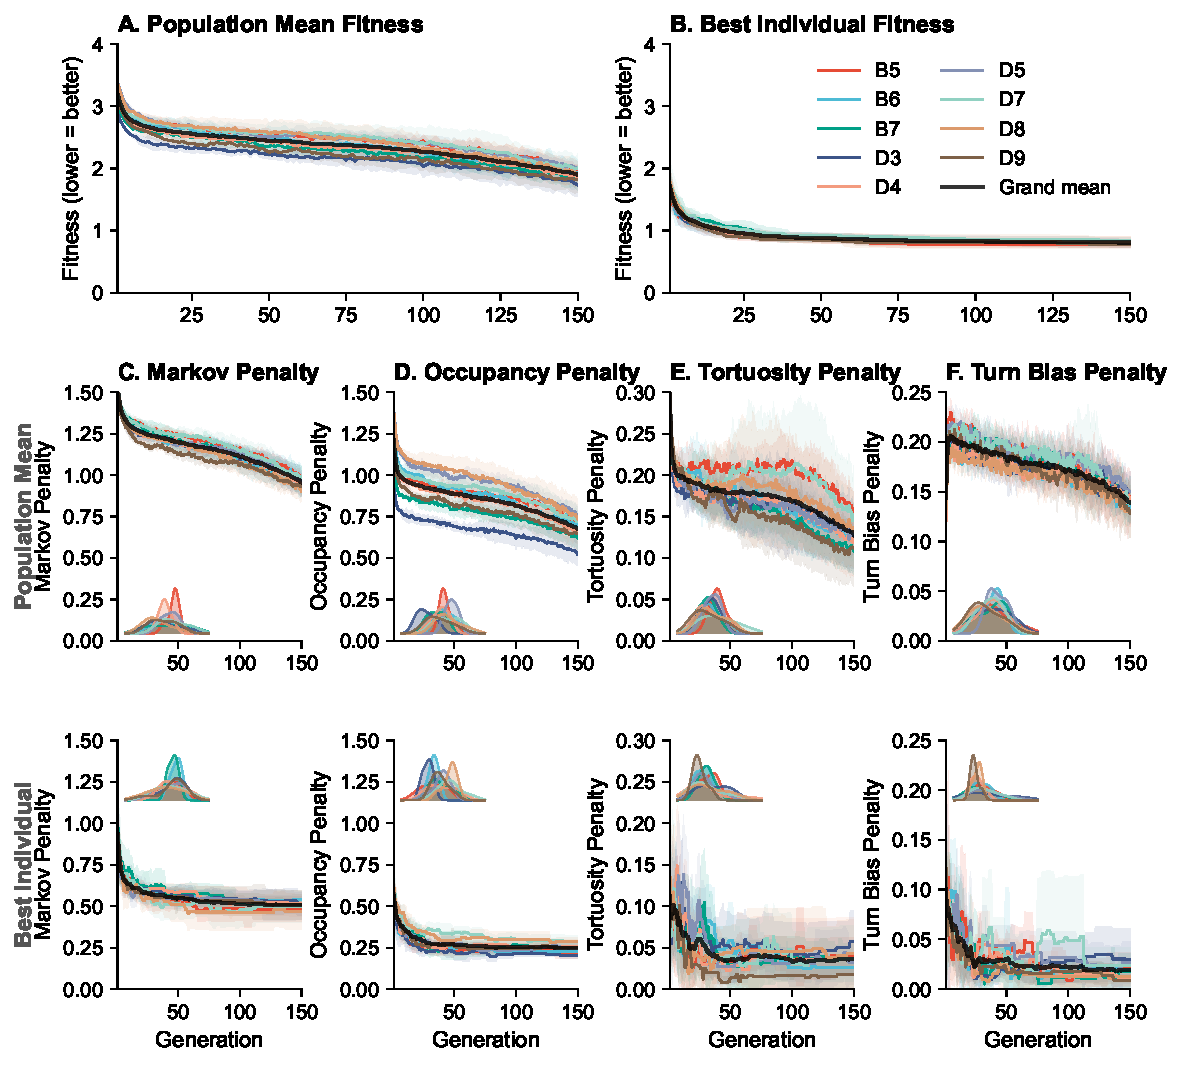
\includegraphics[width=\textwidth]{fig1_permouse.pdf}
  \caption{\textbf{Per-metric evolutionary convergence across 9 mice.}
  (A)~Population mean total fitness (all mice, 6 replicates each).
  (B)~Best individual total fitness.
  (C--F)~Population mean fitness (top sub-row) and best-of-generation fitness
  (bottom sub-row) for each of the four behavioral components: Markov (C),
  Occupancy (D), Tortuosity (E), Turn Bias (F). KDE insets show the
  generation-150 fitness distribution per mouse. Lower = better match.}
  \label{fig:supp_convergence_permouse}
\end{figure}

\subsection*{S3b. Evolved vs random circuit features (numerical summary)}
\label{sec:supp_evr_table}

Table~\ref{tab:evolved_vs_random} lists the seven key structural features from
Figure~\ref{fig:system}G with exact means, Cohen's $d$, and $p$-values for reference.
The forest plot (Figure~\ref{fig:system}G) shows all 18 features with 95\% bootstrap CIs.

\begin{table}[H]
  \centering
  \small
  \caption{\textbf{Evolved vs random circuit features (selected).} One-sample $t$-test
  (evolved values vs random mean; $n_\text{evolved} = 54$, $n_\text{random} = 200$).
  Cohen's $d$ measures effect size (positive = evolved $>$ random). Full 18-feature
  comparison with bootstrap CIs is shown in Figure~\ref{fig:system}G.}
  \label{tab:evolved_vs_random}
  \begin{tabular}{lccrr}
    \toprule
    Feature & Evolved & Random & Cohen's $d$ & $p$ \\
    \midrule
    Total connections          & \statEvolvedVsRandomNConnectionsEvolvedMean & \statEvolvedVsRandomNConnectionsRandomMean & $\statEvolvedVsRandomNConnectionsD$ & \statEvolvedVsRandomNConnectionsP \\
    Sensory-to-motor shortcuts & \statEvolvedVsRandomSmCountEvolvedMean      & \statEvolvedVsRandomSmCountRandomMean      & $+\statEvolvedVsRandomSmCountD$    & \statEvolvedVsRandomSmCountP \\
    Inter-to-motor connections & \statEvolvedVsRandomImCountEvolvedMean      & \statEvolvedVsRandomImCountRandomMean      & $\statEvolvedVsRandomImCountD$     & \statEvolvedVsRandomImCountP \\
    Motor-to-motor connections & \statEvolvedVsRandomMmCountEvolvedMean      & \statEvolvedVsRandomMmCountRandomMean      & $\statEvolvedVsRandomMmCountD$     & \statEvolvedVsRandomMmCountP \\
    Mean weight magnitude      & \statEvolvedVsRandomWMeanMagEvolvedMean     & \statEvolvedVsRandomWMeanMagRandomMean     & $+\statEvolvedVsRandomWMeanMagD$   & \statEvolvedVsRandomWMeanMagP \\
    Fraction at max weight     & \statEvolvedVsRandomFracStrongEvolvedPct\%  & \statEvolvedVsRandomFracStrongRandomPct\%  & $+\statEvolvedVsRandomFracStrongD$ & \statEvolvedVsRandomFracStrongP \\
    Interneuron mean fan-in    & \statEvolvedVsRandomInterInMeanEvolvedMean  & \statEvolvedVsRandomInterInMeanRandomMean  & $\statEvolvedVsRandomInterInMeanD$ & \statEvolvedVsRandomInterInMeanP \\
    \bottomrule
  \end{tabular}
\end{table}

% ----------------------------------------------------------------------------
\subsection*{S4. Emergent behavioral properties: comparison to real mice}
\label{sec:supp_emergent}

Thigmotaxis (wall contact fraction), median speed, and mean absolute turn rate
were computed for all 54 best-evolved agents and compared to their target mouse.
Each property was reproduced without explicit selection: evolved agents were not
optimised for wall proximity, speed magnitude, or turn rate, yet all three
statistics fall within the range of real mouse values across all 9 mice
(Figure~\ref{fig:supp_emergent}). Speed and turn rate distribution panels
appear in Figure~\ref{fig:system}F--G in the main text.

\begin{figure}[H]
  \centering
  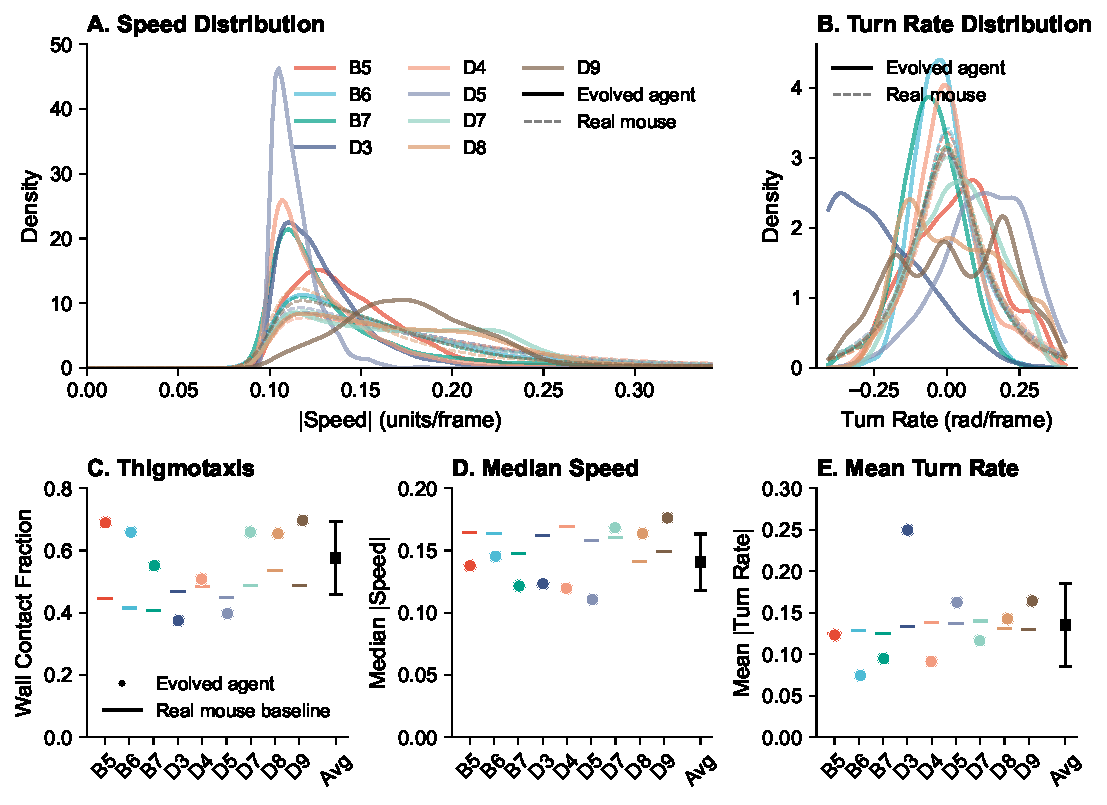
\includegraphics[width=\textwidth]{fig2_permouse.pdf}
  \caption{\textbf{Emergent behavioral properties per mouse (panels C--E).}
  Panels A--B (speed and turn rate distributions) appear in
  Figure~\ref{fig:system}F--G.
  (C)~Wall contact fraction (thigmotaxis): strip plots for evolved replicates
  (dots) overlaid on real mouse baseline (horizontal line).
  (D)~Median speed. (E)~Mean absolute turn rate.
  In all panels, evolved agent values bracket the real mouse value, confirming
  that these emergent properties arise from the general behavioral policy.}
  \label{fig:supp_emergent}
\end{figure}

% ----------------------------------------------------------------------------

\subsection*{S5. Excitatory-inhibitory balance dynamics}
\label{sec:supp_ei_dynamics}

Figure~\ref{fig:supp_ei_dynamics} shows the temporal evolution of E/I balance
across generations for interneurons and motor neurons. Interneurons show no
consistent convergence pattern (panel A). The speed motor neuron converges
uniformly to a strongly excitatory-dominated regime (mean $\approx\statEiBalanceSpeedMean$)
across all 9 mice (panel B). The turn motor neuron converges to a more balanced
regime (mean $\approx\statEiBalanceTurnMean$) with greater inter-mouse variability
(panel C). The per-neuron E/I heatmap at generation 150 appears in
Figure~\ref{fig:system}H.

\begin{figure}[H]
  \centering
  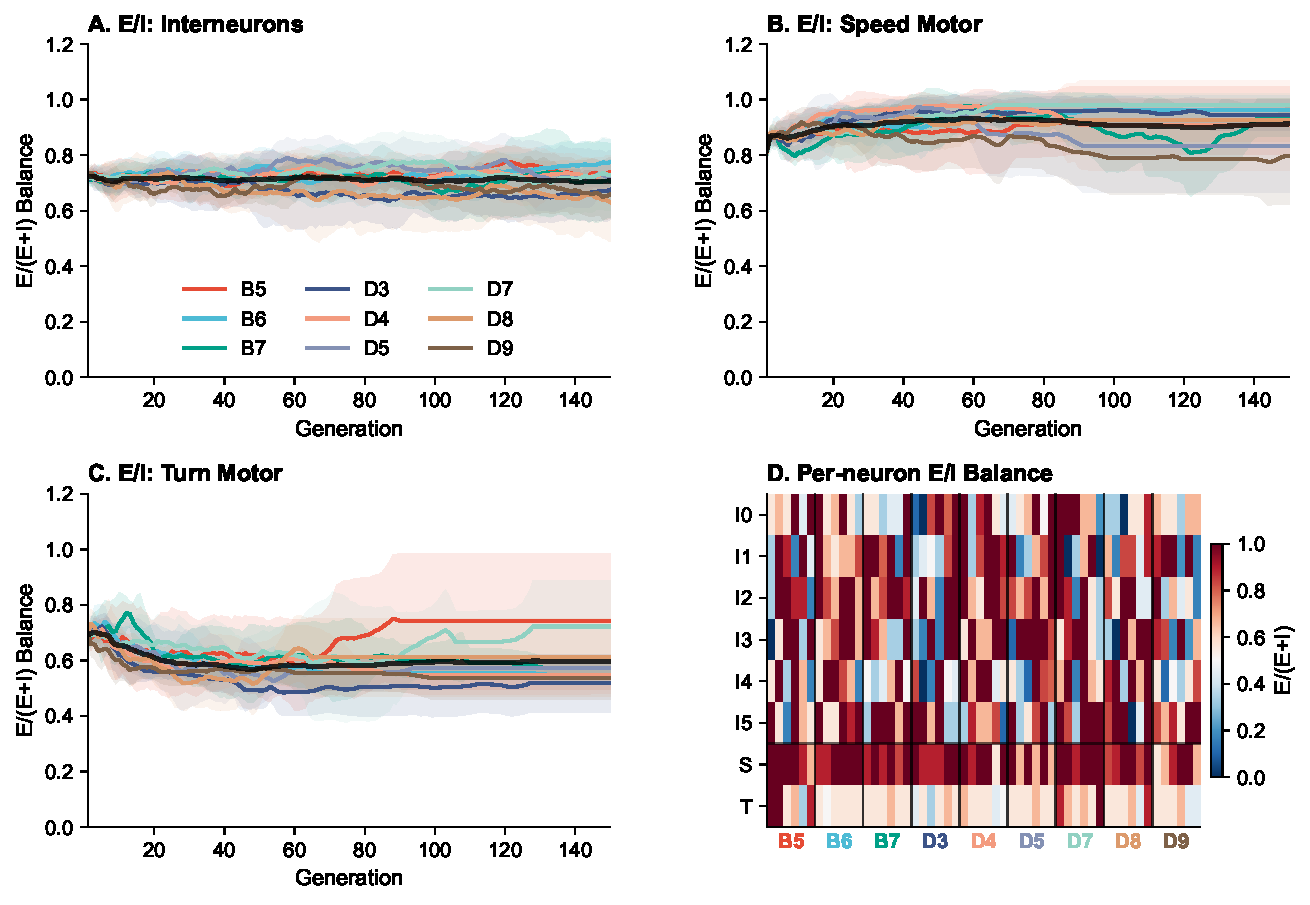
\includegraphics[width=\textwidth]{fig3_network_ei.pdf}
  \caption{\textbf{Excitatory-inhibitory balance dynamics (panels A--C).}
  Panel D (per-neuron E/I heatmap at generation 150) appears in
  Figure~\ref{fig:system}H.
  (A)~E/I balance for all six interneurons over 150 generations (coloured lines
  = per-mouse mean $\pm$SD; black = grand mean). No consistent convergence pattern
  emerges.
  (B)~E/I balance for the speed motor neuron, converging uniformly to
  mean $\approx\statEiBalanceSpeedMean$ excitatory across all 9 mice.
  (C)~E/I balance for the turn motor neuron, converging to
  mean $\approx\statEiBalanceTurnMean$ with greater variability, consistent with
  closed-loop inhibitory modulation of turning direction.}
  \label{fig:supp_ei_dynamics}
\end{figure}

% ----------------------------------------------------------------------------

\subsection*{S6. Evolved vs random weight similarity distributions}
\label{sec:supp_cosine_dist}

\begin{figure}[H]
  \centering
  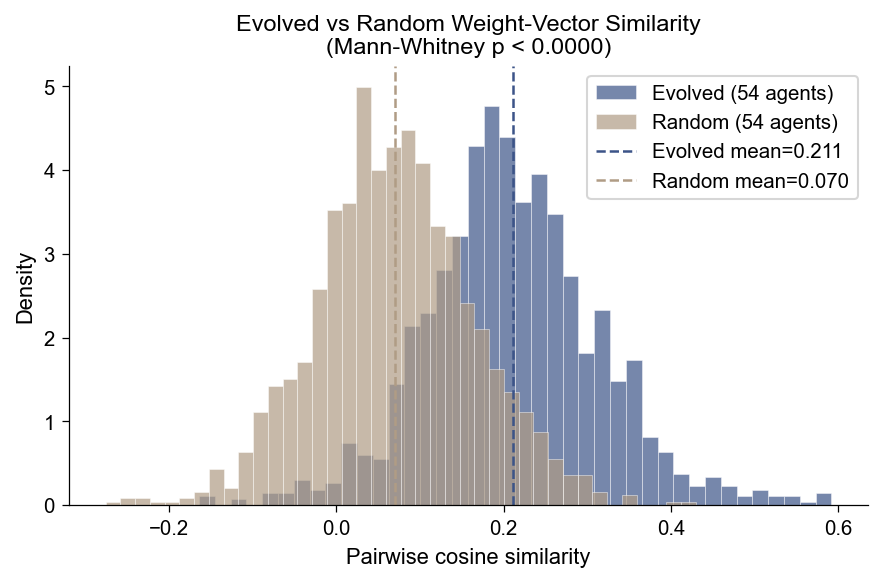
\includegraphics[width=0.65\textwidth]{fig_c1_cosine_evolved_vs_random.png}
  \caption{\textbf{Evolved circuits occupy a significantly narrower region of
  weight space than random agents.}
  Pairwise cosine similarity distributions for evolved (blue; $n = 54$) and
  randomly initialised constrained agents (tan; $n = 200$). Evolved mean
  $= \statCosineEvolvedRandomEvolvedMean$; random mean
  $= \statCosineEvolvedRandomRandomMean$; Mann-Whitney
  $p = \statCosineEvolvedRandomMannwhitneyP$. Evolution compresses all circuits
  into a shared structural region, though the $54 \times 54$ similarity matrix
  (Figure~\ref{fig:paradox}A) shows no mouse-level block structure within that
  region.}
  \label{fig:supp_cosine_dist}
\end{figure}

% ----------------------------------------------------------------------------

\subsection*{S7. Power analysis}
\label{sec:supp_power_analysis}

Post-hoc power analysis for the 18-feature ANOVA is shown in
Figure~\ref{fig:supp_power}. At $N = 54$ and $k = 9$ groups, the minimum
detectable $\eta^2$ at 80\% power is $\statPowerTopFeatureMde$. The three
largest-effect features each exceed this threshold (82--88\% power), confirming
the null result is not due to insufficient power for large effects. Medium-effect
features ($\eta^2 \approx \statPowerMedEtaTwoLow$--$\statPowerMedEtaTwoHigh$) would require
$\statPowerRequiredNMedLow$--$\statPowerRequiredNMedHigh$ replicates per mouse.

\begin{figure}[H]
  \centering
  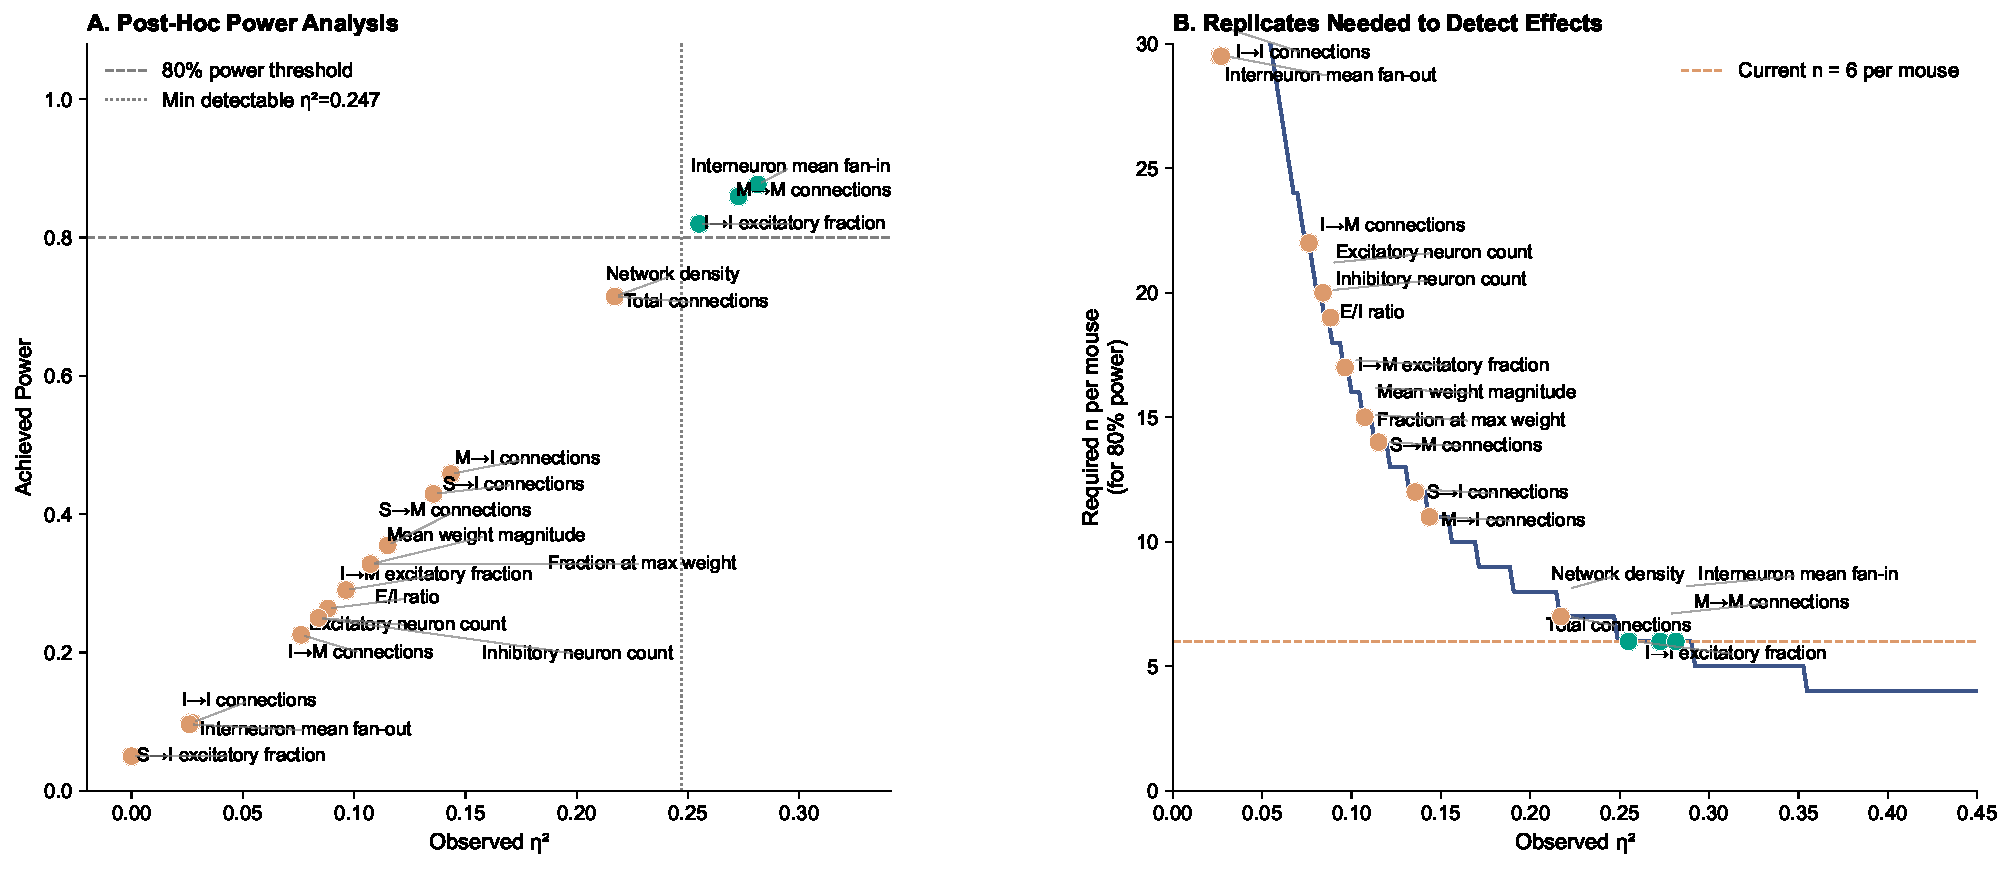
\includegraphics[width=\textwidth]{fig_supp_power_v2.pdf}
  \caption{\textbf{Post-hoc power analysis.}
  (A)~Observed $\eta^2$ vs achieved power. Teal points exceed 80\% power
  threshold; orange points fall below it.
  (B)~Required replicates per mouse for 80\% power at each observed effect size.
  Current $n = 6$ per mouse (dashed orange line) is sufficient for large effects.}
  \label{fig:supp_power}
\end{figure}

\begin{figure}[H]
  \centering
  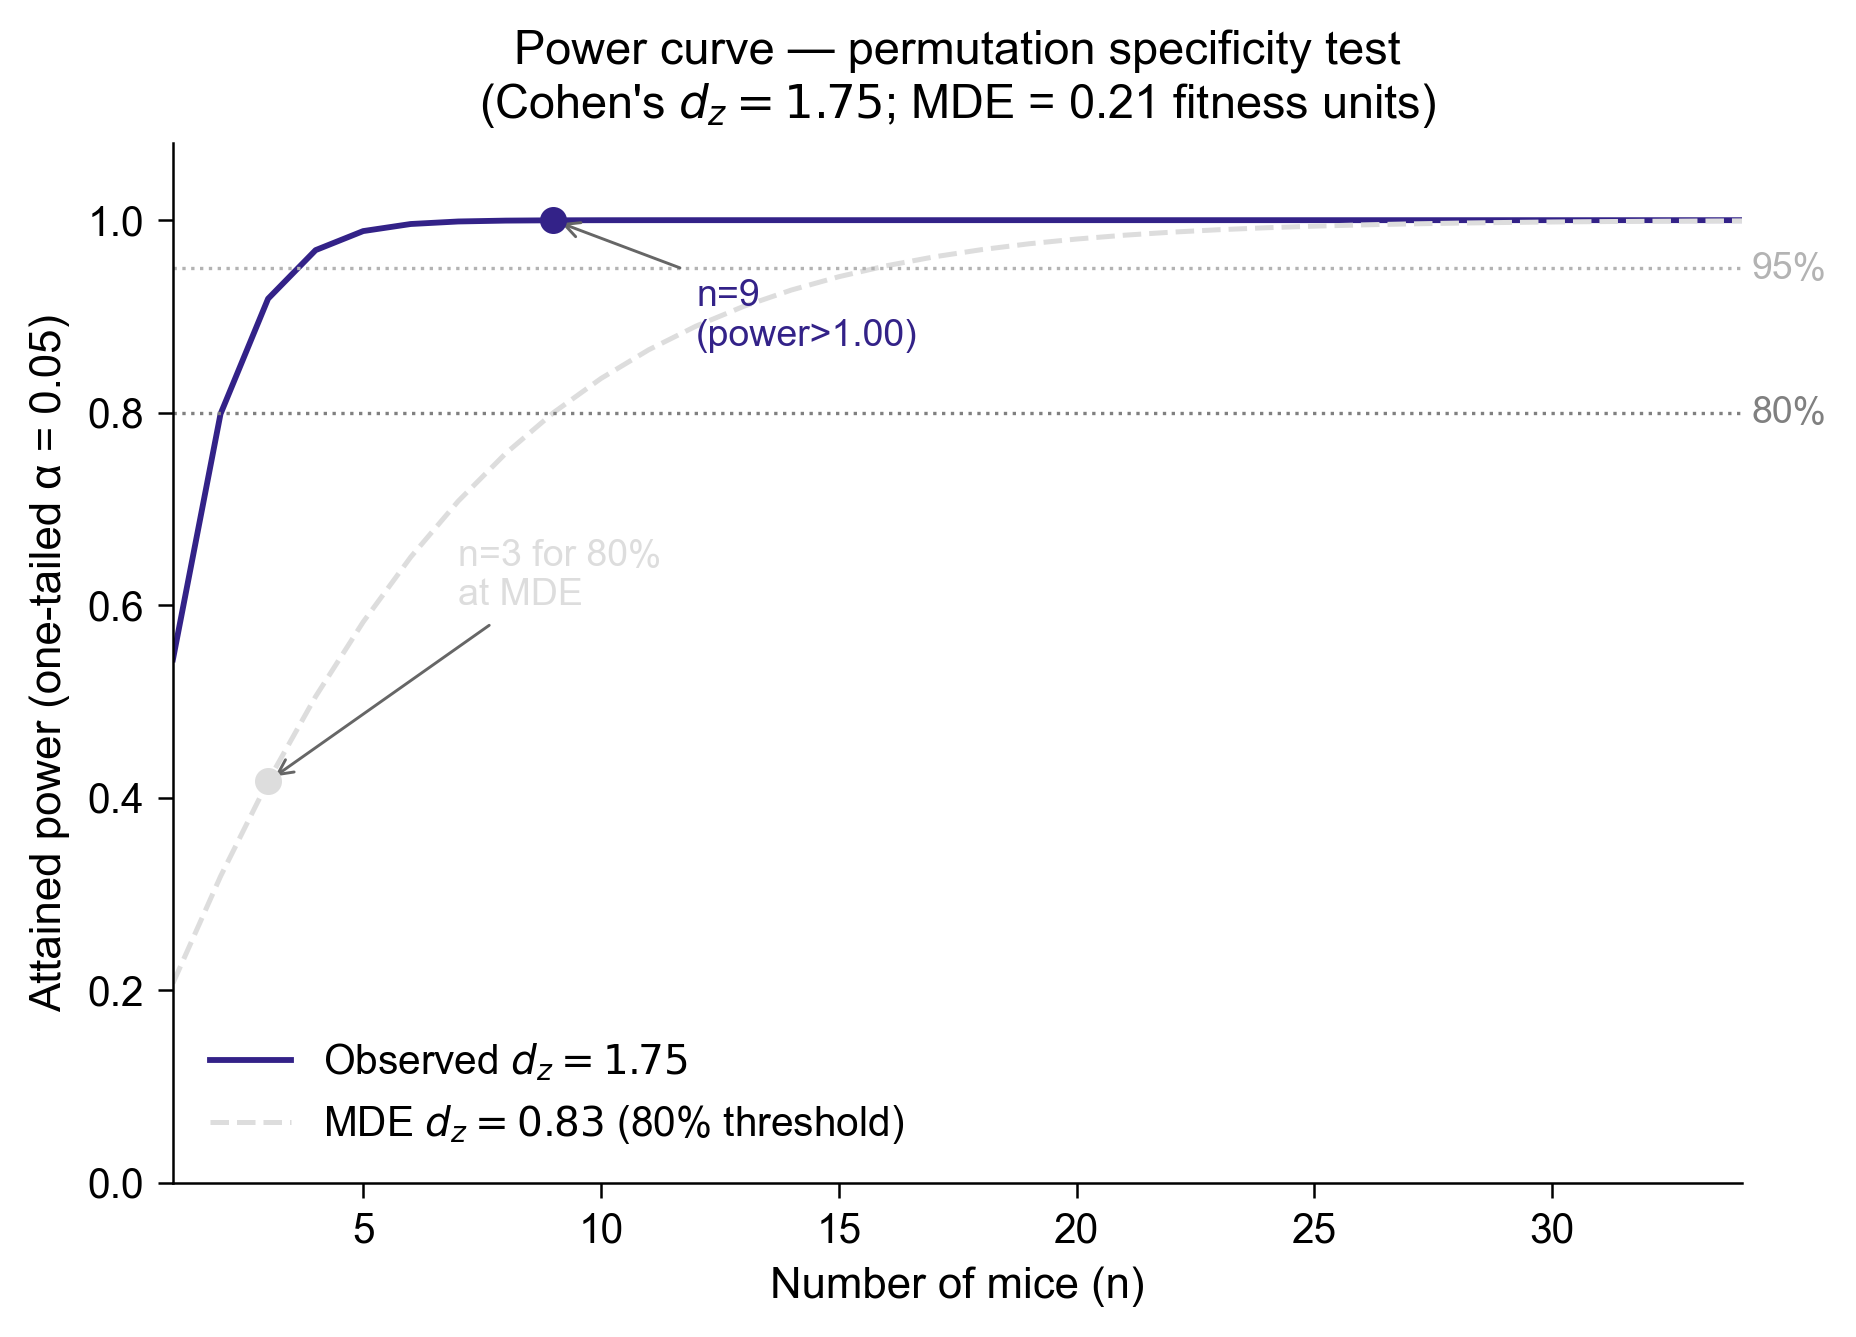
\includegraphics[width=0.6\textwidth]{fig_supp_power_curve.png}
  \caption{\textbf{Power curve.} Required replicates per mouse for 80\%
  power across a range of effect sizes ($\eta^2$).}
  \label{fig:supp_power_curve}
\end{figure}

% ----------------------------------------------------------------------------

\subsection*{S8. Per-metric specialisation: cross-evaluation heatmaps}

The cross-evaluation structure visible in the total fitness matrix
(Figure~\ref{fig:paradox}D) replicates independently within each fitness
component. Each of the four per-metric $9 \times 9$ matrices shows the same
diagonal pattern: agents consistently achieve lower error on their own target
mouse than on other mice
(Figure~\ref{fig:supp_per_metric_heatmaps}).

\begin{figure}[H]
  \centering
  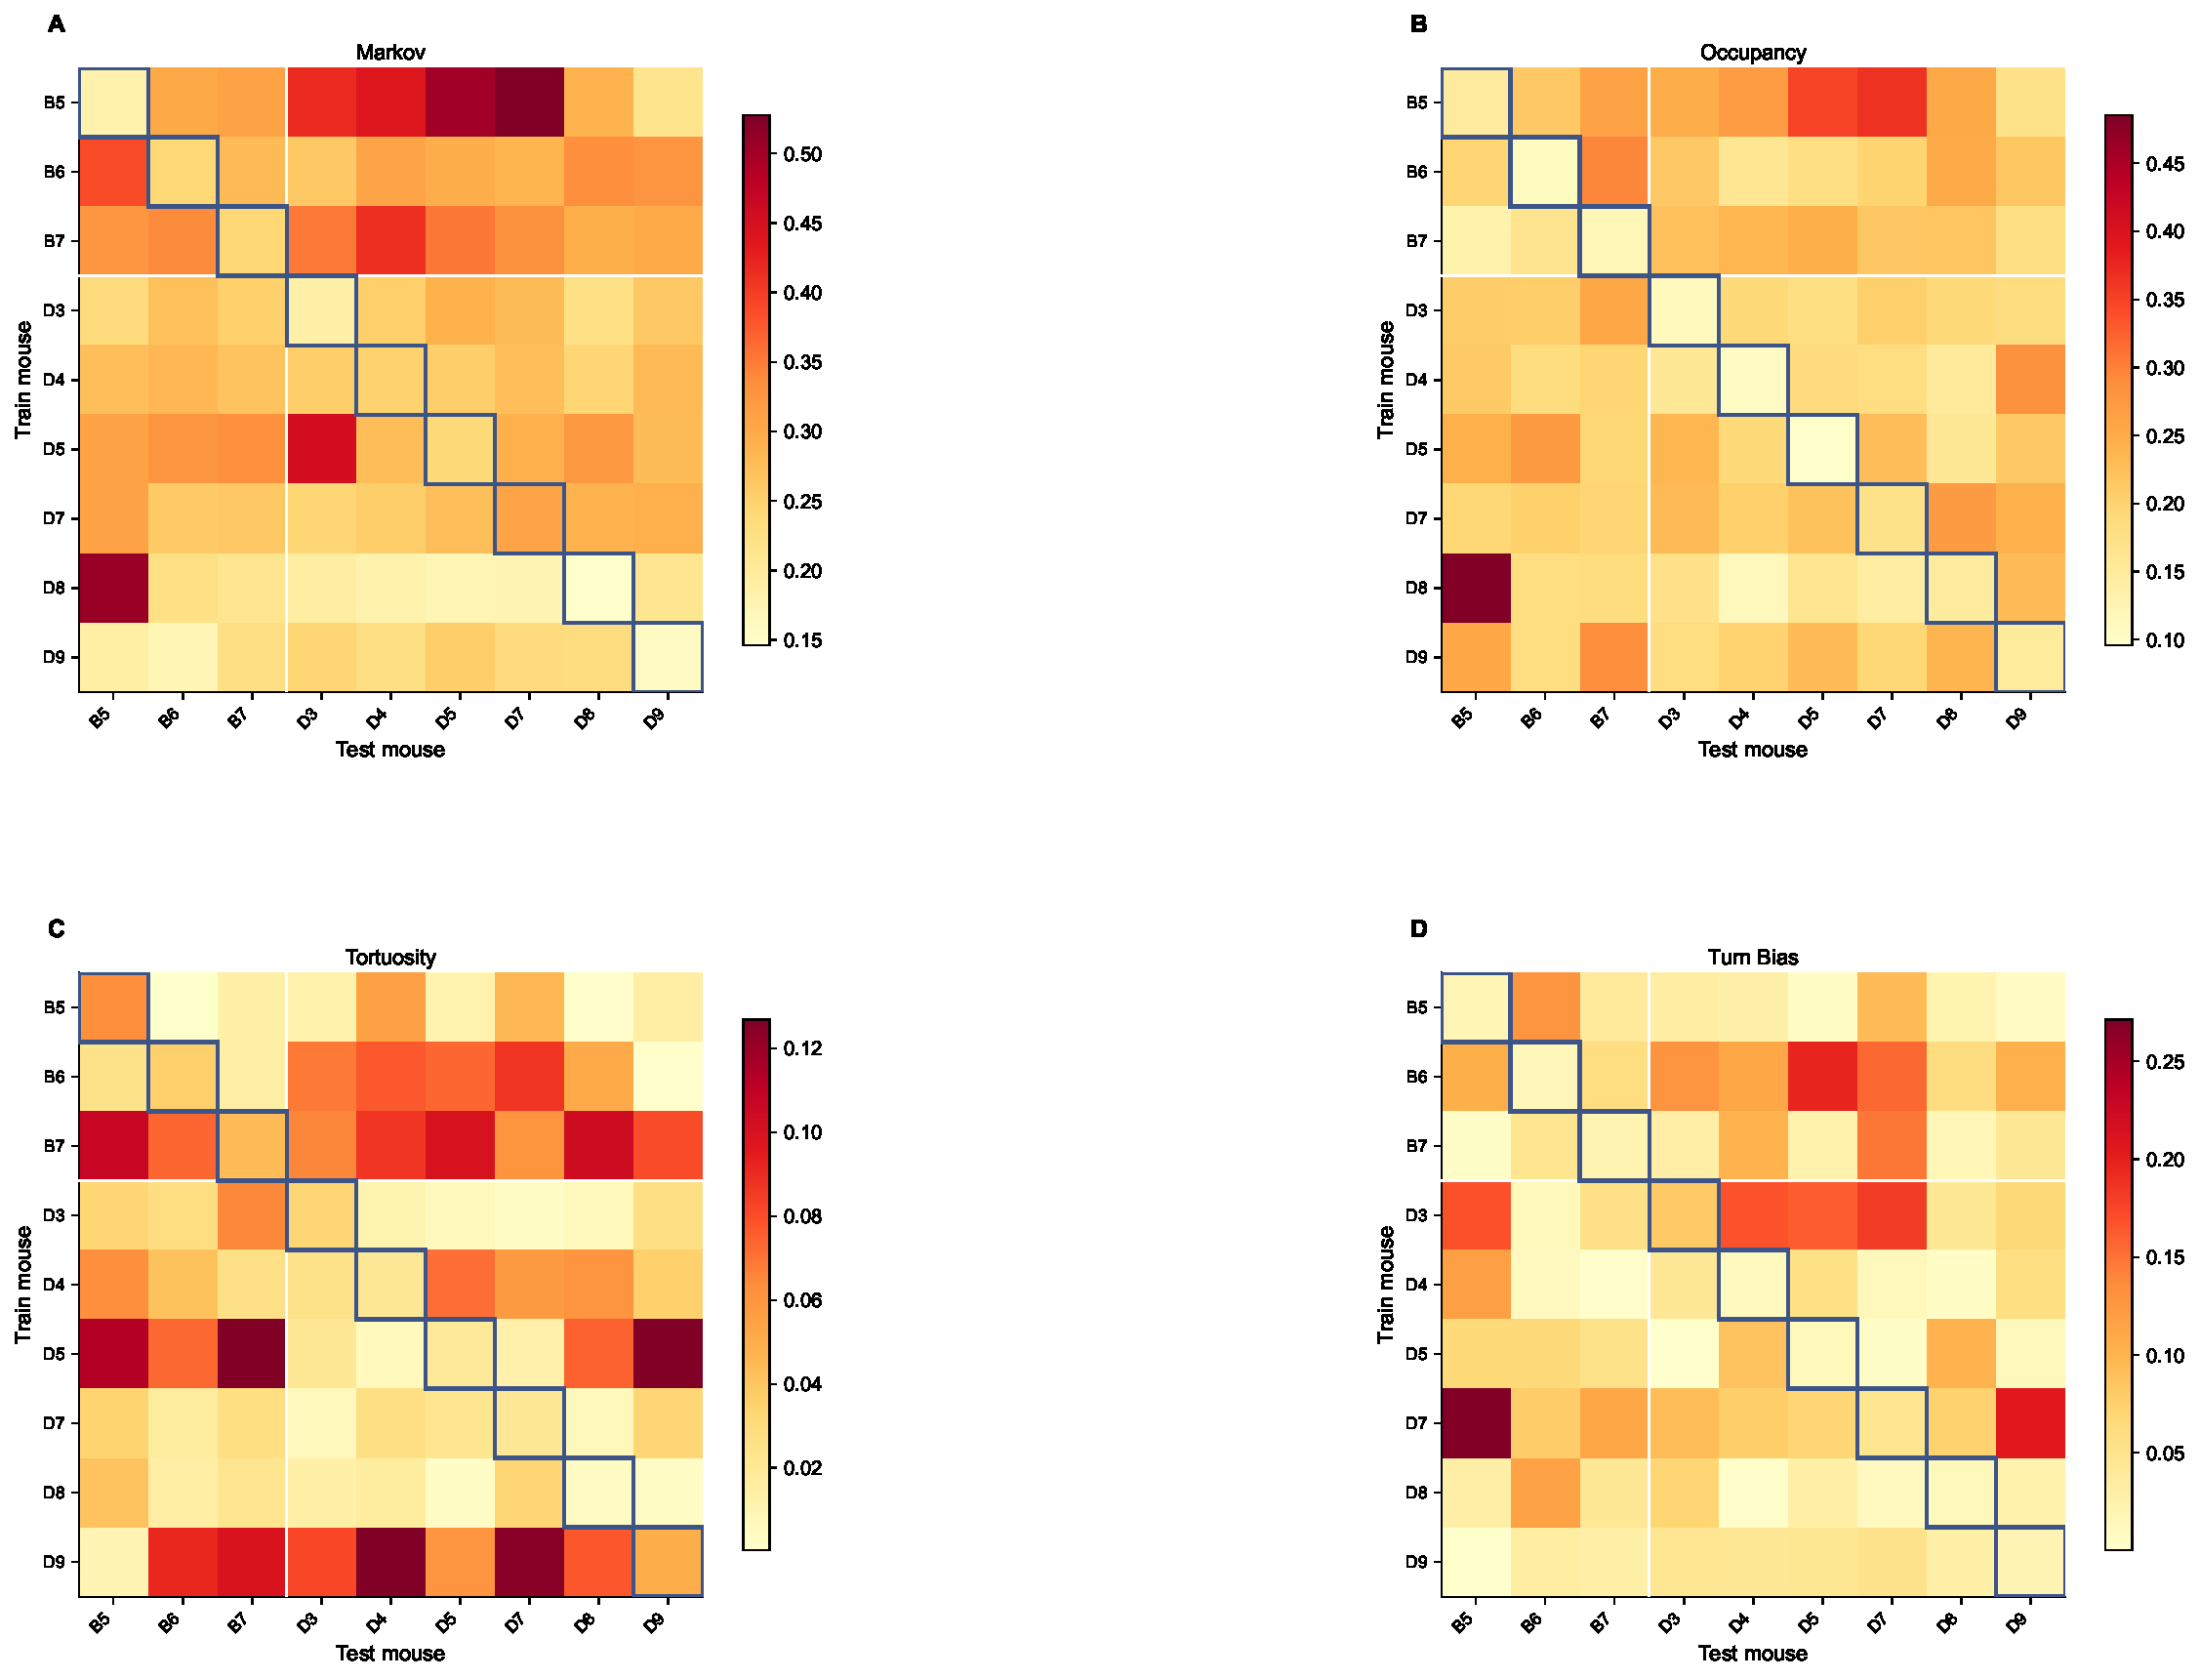
\includegraphics[width=\textwidth]{fig_per_metric_crosseval.pdf}
  \caption{\textbf{Per-metric $9 \times 9$ cross-evaluation matrices.}
  Each panel shows the cross-evaluation fitness matrix for one of the four
  behavioural components (Markov, Occupancy, Tortuosity, Turn Bias).
  Colour encodes component fitness error (lower = better match). Blue boxes
  mark diagonal (own-mouse) entries. The diagonal specialisation structure
  replicates independently in every component.}
  \label{fig:supp_per_metric_heatmaps}
\end{figure}

% ----------------------------------------------------------------------------

\subsection*{S9. Per-metric specialisation: own vs cross-mouse bars}

Cross-mouse error exceeds own-mouse error in every fitness component; the
own/cross ratio ranges from $\statPerMetricTurnBiasRatio$ (turn bias, most
individual-specific) to $\statPerMetricMarkovRatio$ (Markov transitions;
Figure~\ref{fig:supp_per_metric_bars}).

\begin{figure}[H]
  \centering
  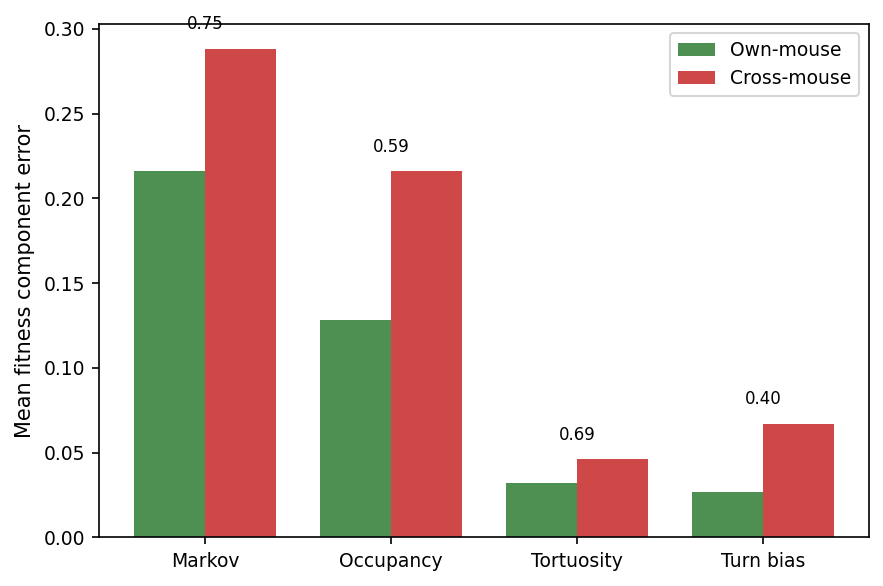
\includegraphics[width=0.75\textwidth]{supp_A6_per_metric.png}
  \caption{\textbf{Own-mouse vs cross-mouse error per fitness component.}
  Mean fitness component error for own-mouse (green) and cross-mouse (red)
  evaluations, averaged across all 9 mice. Ratio annotated above each
  cross-mouse bar (own/cross; lower = more specialised). Turn bias shows
  the strongest individual-specificity (ratio $= \statPerMetricTurnBiasRatio$),
  followed by occupancy ($\statPerMetricOccupancyRatio$), tortuosity
  ($\statPerMetricTortuosityRatio$), and Markov transitions
  ($\statPerMetricMarkovRatio$).}
  \label{fig:supp_per_metric_bars}
\end{figure}

% ----------------------------------------------------------------------------

\subsection*{S10. Strain control}

Specialisation indices computed within each genetic strain independently
(B-strain: $\statStrainConfoundBRatio$; D-strain: $\statStrainConfoundDRatio$)
remain close to the overall index ($\statCrossMouseSpecIndex$), confirming that
individual-level behavioral divergence is present within each strain and is not
an artefact of between-strain differences (Figure~\ref{fig:supp_strain}).

\begin{figure}[H]
  \centering
  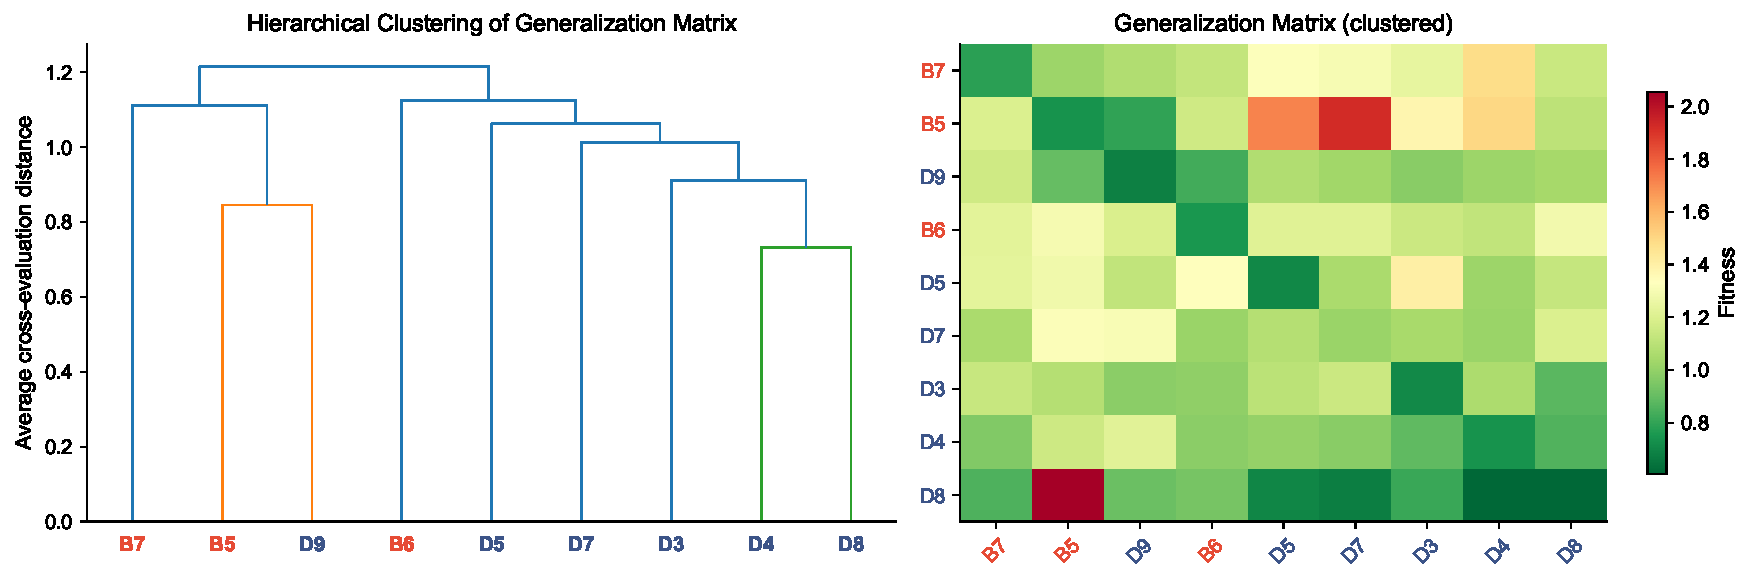
\includegraphics[width=0.7\textwidth]{strain_clustering.pdf}
  \caption{\textbf{Strain control.} Specialisation indices within B-strain and
  D-strain mice remain positive and close to the overall index.}
  \label{fig:supp_strain}
\end{figure}

% ----------------------------------------------------------------------------

\subsection*{S11. Fitness weighting scheme robustness}

The specialisation index was recomputed under five alternative fitness weighting
schemes for the four behavioral components (Markov, Occupancy, Tortuosity,
Turn Bias). All five schemes produce positive mean indices
(Table~\ref{tab:supp_weighting}; Figure~\ref{fig:supp_weighting_schemes}),
confirming the finding is not sensitive to the choice of component weights.

\begin{table}[H]
  \centering
  \small
  \caption{\textbf{Specialisation index under five fitness weighting schemes.}
  The primary analysis uses the Published 2:2:1:1 scheme. Per-mouse breakdown
  is shown in Figure~\ref{fig:supp_weighting_schemes}.}
  \label{tab:supp_weighting}
  \begin{tabular}{lcc}
    \toprule
    Weighting scheme & Mean specialisation index & Mice $> 0$ \\
    \midrule
    Published (2:2:1:1)       & $\statCrossMouseSpecIndex$         & $\statSensitivityPublishedNPos$/9 \\
    Equal (1:1:1:1)           & $\statSensitivityEqualWeightIndex$ & $\statSensitivityEqualWeightNPos$/9 \\
    Turn-dominant (1:1:1:3)   & $\statSensitivityTurnDomIndex$     & $\statSensitivityTurnDomNPos$/9 \\
    Markov-only (1:0:0:0)     & $\statSensitivityMarkovOnlyIndex$  & $\statSensitivityMarkovOnlyNPos$/9 \\
    Turn+Occupancy (0:2:0:1)  & $\statSensitivityOccTurnIndex$     & $\statSensitivityOccTurnNPos$/9 \\
    \bottomrule
  \end{tabular}
\end{table}

\begin{figure}[H]
  \centering
  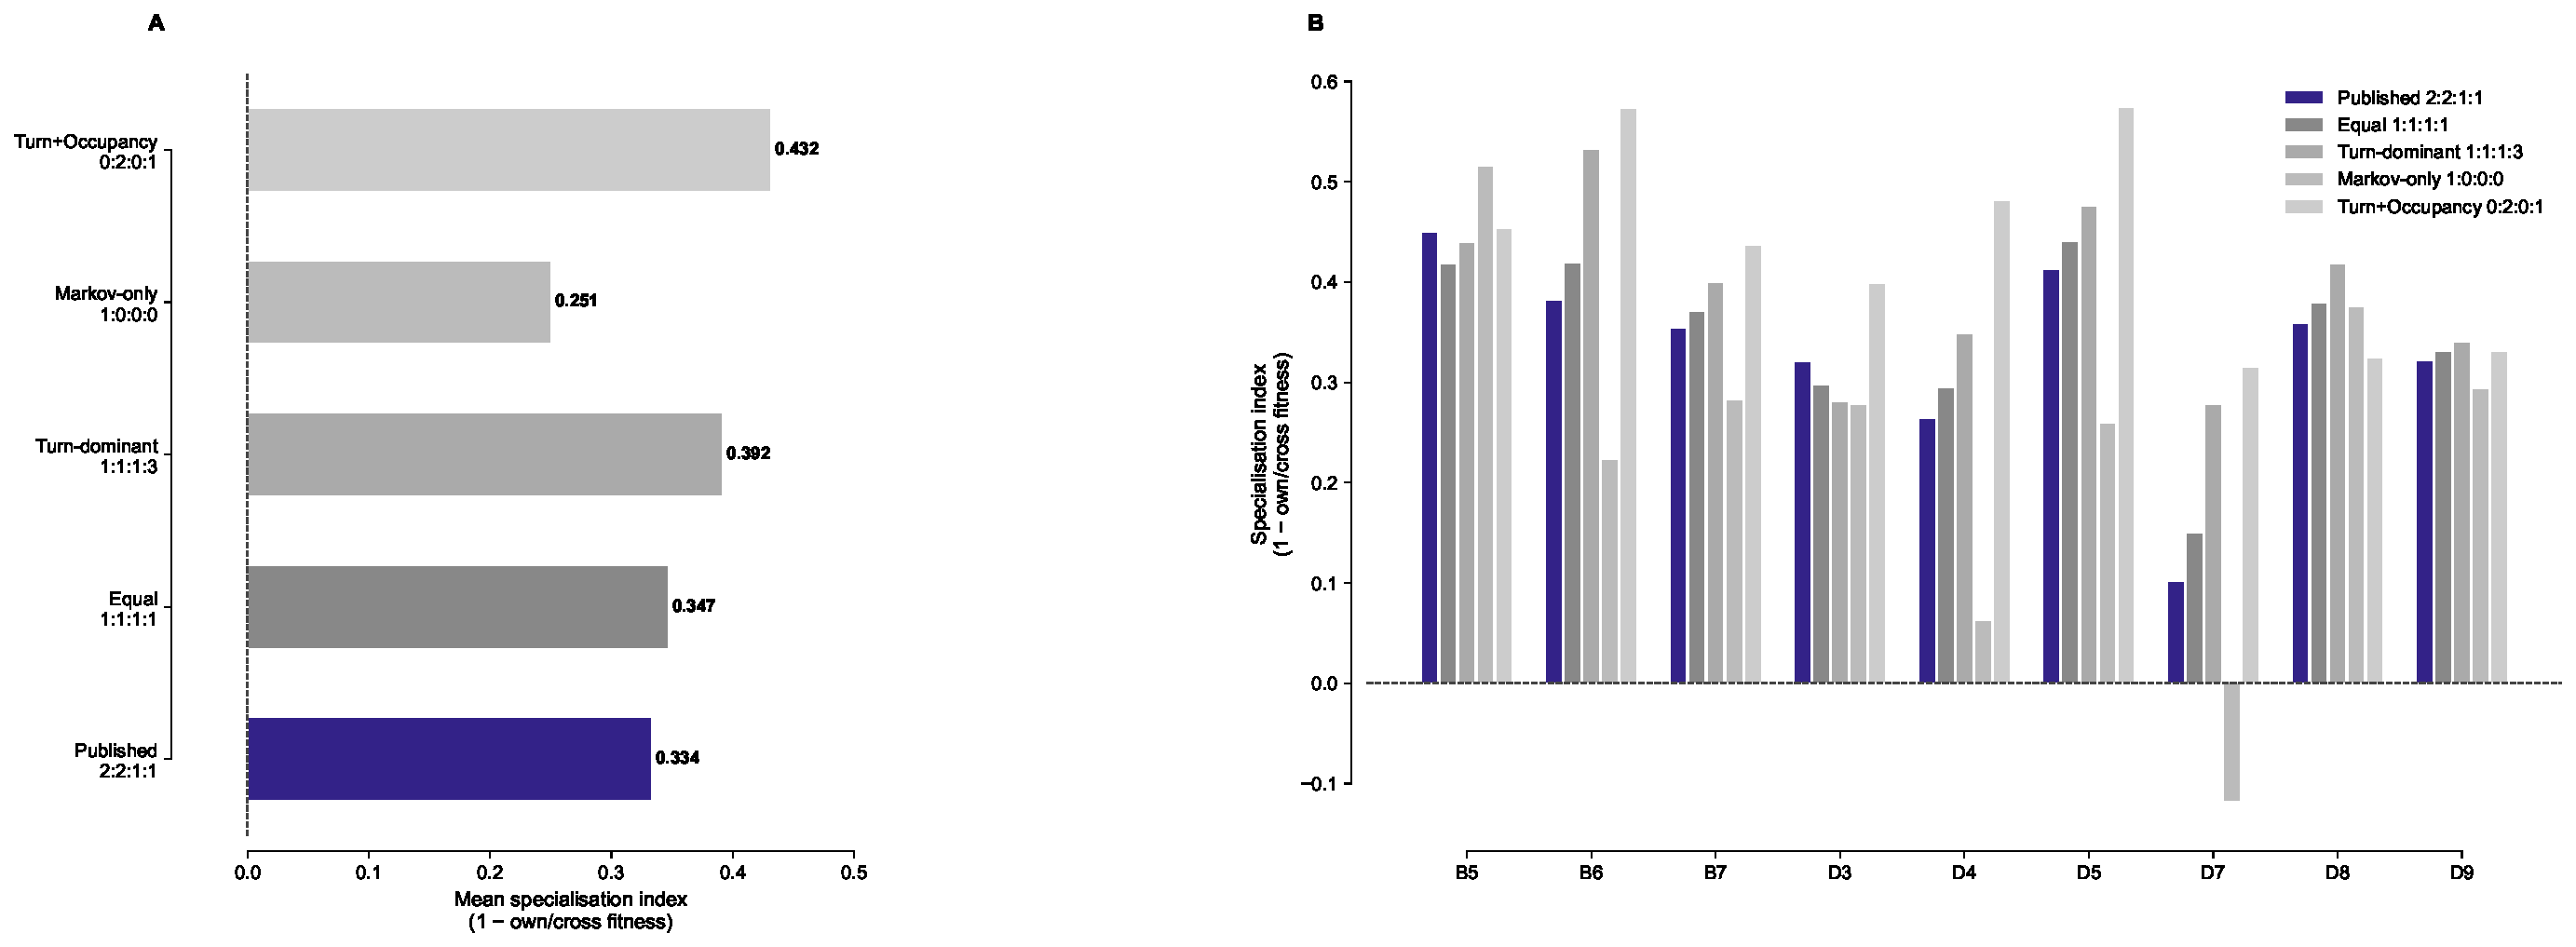
\includegraphics[width=\textwidth]{supp_s_weighting.pdf}
  \caption{\textbf{Specialisation index is robust to fitness weighting choice.}
  (A)~Mean specialisation index ($1 - \text{own/cross fitness}$) across all 9 mice
  for each of five weighting schemes. Published 2:2:1:1 (highlighted) is the
  primary analysis; dashed line at zero indicates no specialisation.
  (B)~Per-mouse specialisation index for all 9 mice across the five schemes.
  All schemes produce positive mean indices.}
  \label{fig:supp_weighting_schemes}
\end{figure}

% ----------------------------------------------------------------------------

\subsection*{S12. Specialisation persists on held-out behavioral data}
\label{sec:supp_holdout}

Behavioral baseline and fitness evaluation used the same trajectory bouts from
each mouse's recording. To test whether specialisation reflects genuine
individual-level encoding rather than bout-specific fitting, we performed
cross-bout evaluation using the second half of each mouse's trajectory as a
held-out test set.

The held-out specialisation index was $\statHoldoutHoldoutIndex$ across all 9
mice (all held-out indices $> 0$; Figure~\ref{fig:supp_holdout}), compared to
$\statHoldoutTrainingIndex$ on the training set. The attenuation reflects
reduced statistical precision of the held-out behavioral baseline rather than
overfitting: each mouse's held-out target is estimated from
${\approx}\statHoldoutMeanBoutsHoldout$ trajectory bouts rather than
${\approx}\statHoldoutMeanBoutsTotal$, reducing the resolution of the behavioral
fingerprint. No agent lost specialisation entirely; the unanimous persistence of
positive indices is inconsistent with genuine overfitting.

We confirmed directly, from the real mouse data alone, that the individual
behavioral targets are stably distinguishable beyond within-mouse bout-to-bout
noise (this is the foundation on which the agent-level specialisation rests). We
partitioned each mouse's bouts into $\statIndividuationNFolds$ folds, computed the
four fitness metrics per fold with the same machinery used for fitness, and compared
within- vs between-mouse fold distances. Within-mouse fold distances were smaller than
between-mouse distances in the combined fitness metric (within $=\statIndividuationWithinDist$,
between $=\statIndividuationBetweenDist$; Mann-Whitney $p \statIndividuationMwP$,
rank-biserial $=\statIndividuationRankBiserial$), and a leave-one-fold-out
nearest-mouse classifier reached $\statIndividuationClassAccPct$\% accuracy against a
$\statIndividuationChancePct$\% chance level (permutation $p \statIndividuationClassP$).
The mice are therefore genuinely individuated in the behavioral metrics, so the
held-out attenuation is target-estimation noise, not a circularity of the fitness
definition.

\begin{figure}[H]
  \centering
  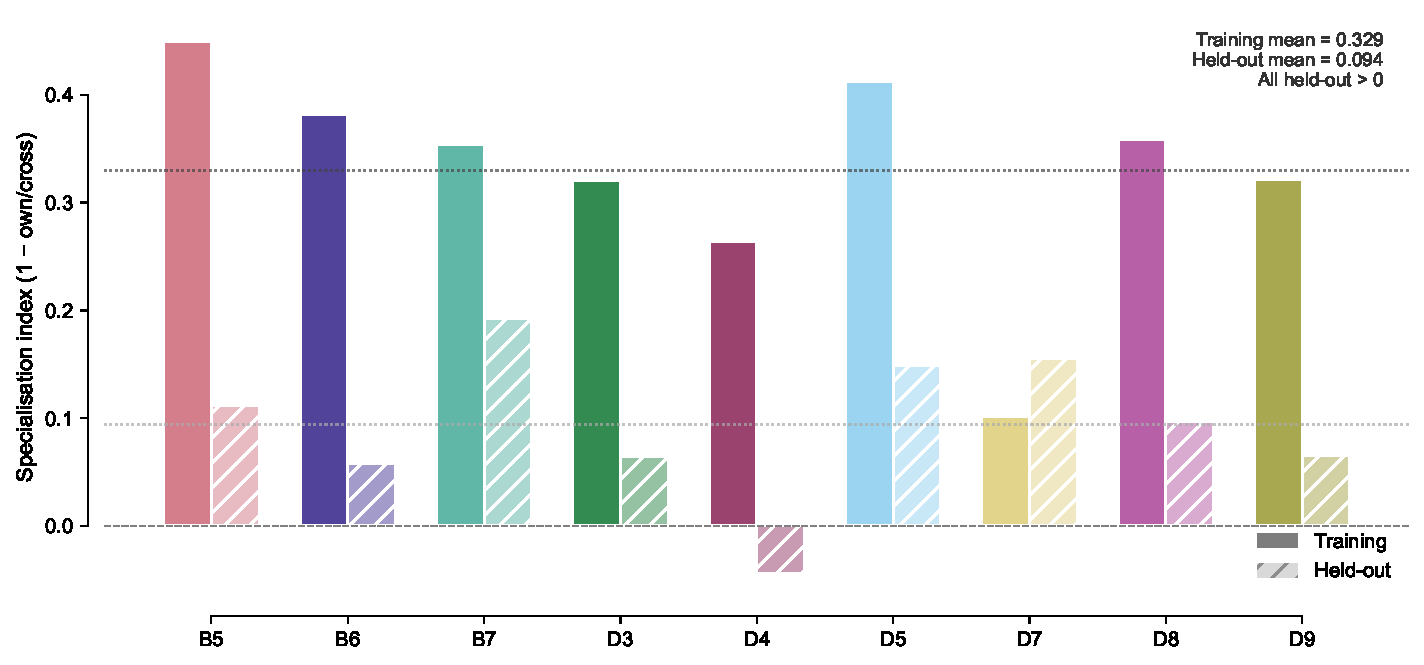
\includegraphics[width=0.85\textwidth]{fig_supp_holdout.pdf}
  \caption{\textbf{Holdout specialisation indices per mouse.}
  Paired bars showing training-set (solid) and held-out (hatched) specialisation
  indices for each of the 9 mice, coloured by mouse identity. All held-out
  indices are positive (population mean $= \statHoldoutHoldoutIndex$), confirming
  that specialisation generalises across trajectory bouts. The attenuation
  relative to training ($\statHoldoutTrainingIndex$) reflects reduced bout
  count in the held-out half, not overfitting.}
  \label{fig:supp_holdout}
\end{figure}

% ----------------------------------------------------------------------------

\subsection*{S12b. Per-source ablation sensitivity (null result)}
\label{sec:supp_ablation_heatmap}

Permuting each source neuron's outgoing connections individually, rather than
the full topology at once, yields a $54 \times 14$ sensitivity matrix
(Figure~\ref{fig:supp_ablation_heatmap}). Agents are ordered by mouse (six
replicates per mouse, separated by white lines). No mouse-level block structure
is visible: 0 of 14 source neurons reach significance after Bonferroni
correction, and within-mouse sensitivity profiles are no more correlated than
between-mouse profiles ($r_\text{within} = \statSourceSensitivityWithinRMean$,
$r_\text{between} = \statSourceSensitivityBetweenRMean$,
Mann-Whitney $p = \statSourceSensitivityMwP$). Individual source neurons do not
fingerprint mouse identity, even though the full topology is causally necessary.

\begin{figure}[H]
  \centering
  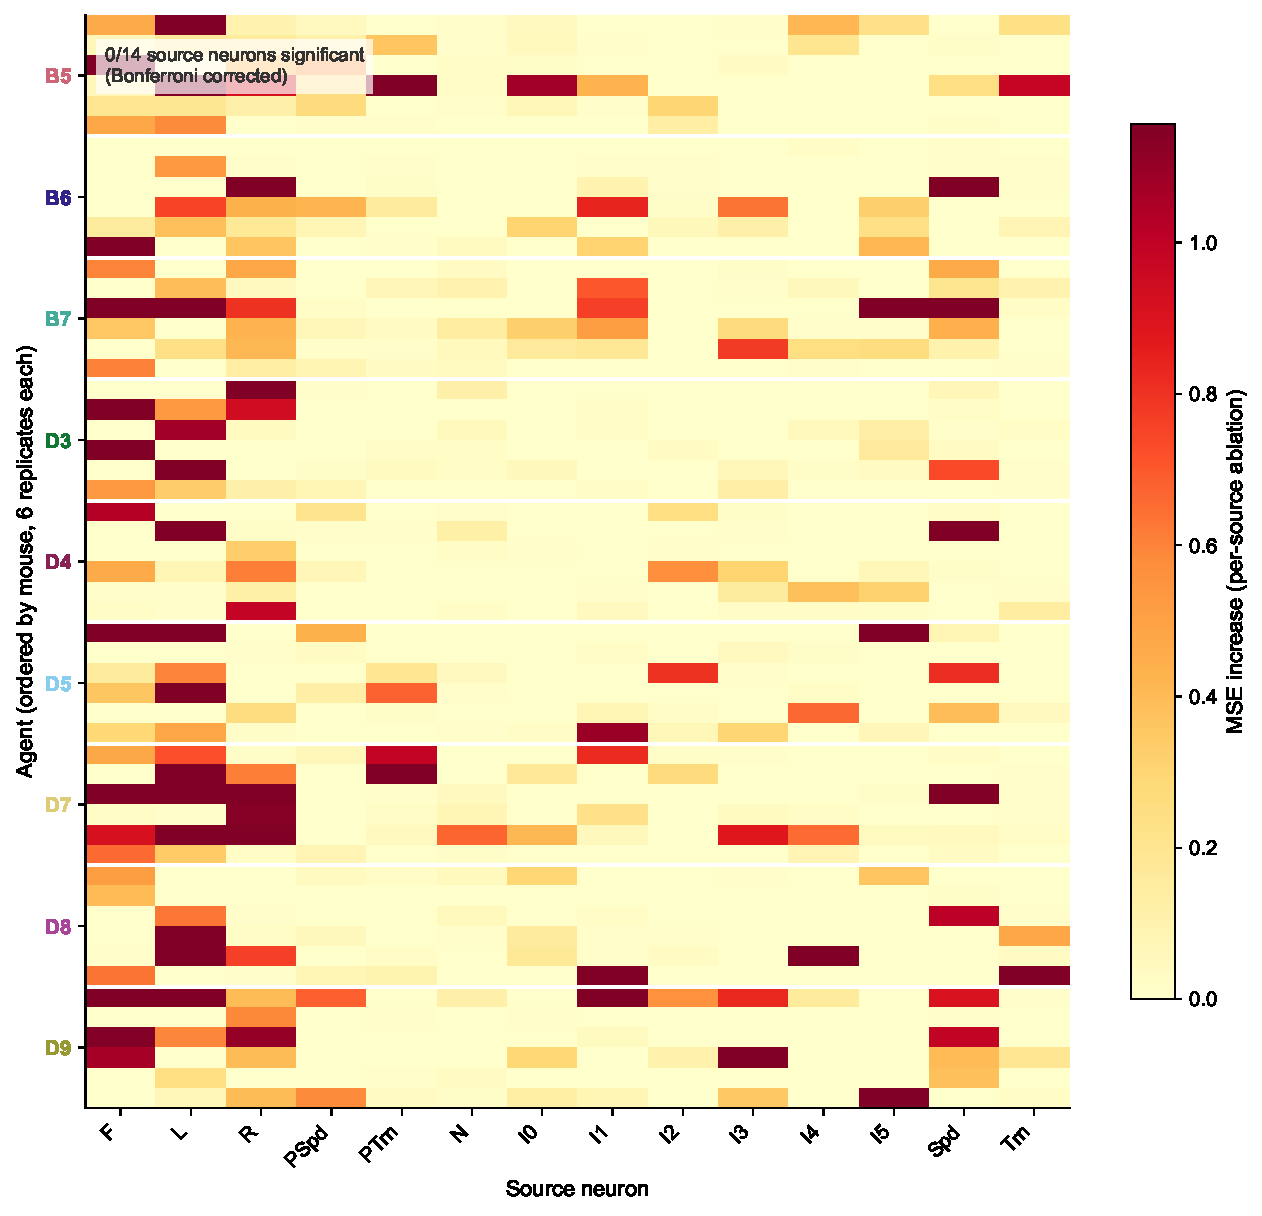
\includegraphics[width=0.75\textwidth]{fig_supp_ablation_heatmap.pdf}
  \caption{\textbf{Per-source ablation sensitivity matrix (54 agents $\times$ 14
  source neurons).} Each cell shows the increase in motor output MSE when that
  source neuron's outgoing connections are permuted individually. Agents are
  ordered by mouse (white separator lines every 6 rows). No mouse-level block
  structure is visible; 0/14 source neurons reach significance after Bonferroni
  correction.}
  \label{fig:supp_ablation_heatmap}
\end{figure}

% ----------------------------------------------------------------------------

\subsection*{S13. Structural clustering visualization: k-means groups do not correspond to mouse identity or performance}
\label{sec:supp_mi_clustering}

The mutual information analysis of Section~\ref{sec:mi} groups each of the 54 agents
into one of $k = 5$ structural clusters via k-means, separately for each structural
axis, and measures how well these cluster labels predict mouse identity. Figure~\ref{fig:supp_mi_clustering}
shows two complementary views of why these structural clusters carry no behavioral information.

Panels A and B show the same PCA embedding of agents in topology feature space with
different color encodings. Panel A colors by k-means cluster: five structural groups are
present in the data. Panel B colors the same points by mouse identity: agents from the same mouse
are scattered across all five clusters, and each cluster contains agents from multiple mice.
Panel C replicates the null on the magnitude axis: mouse identity is equally unrecoverable
from structural similarity in magnitude space. Panel D provides the fitness-quintile
companion analysis: agents ranked by own-mouse fitness (best on left), colored by
topology cluster. If structurally similar agents performed similarly, colors would grade
smoothly across the rank axis; they do not.

\begin{figure}[H]
  \centering
  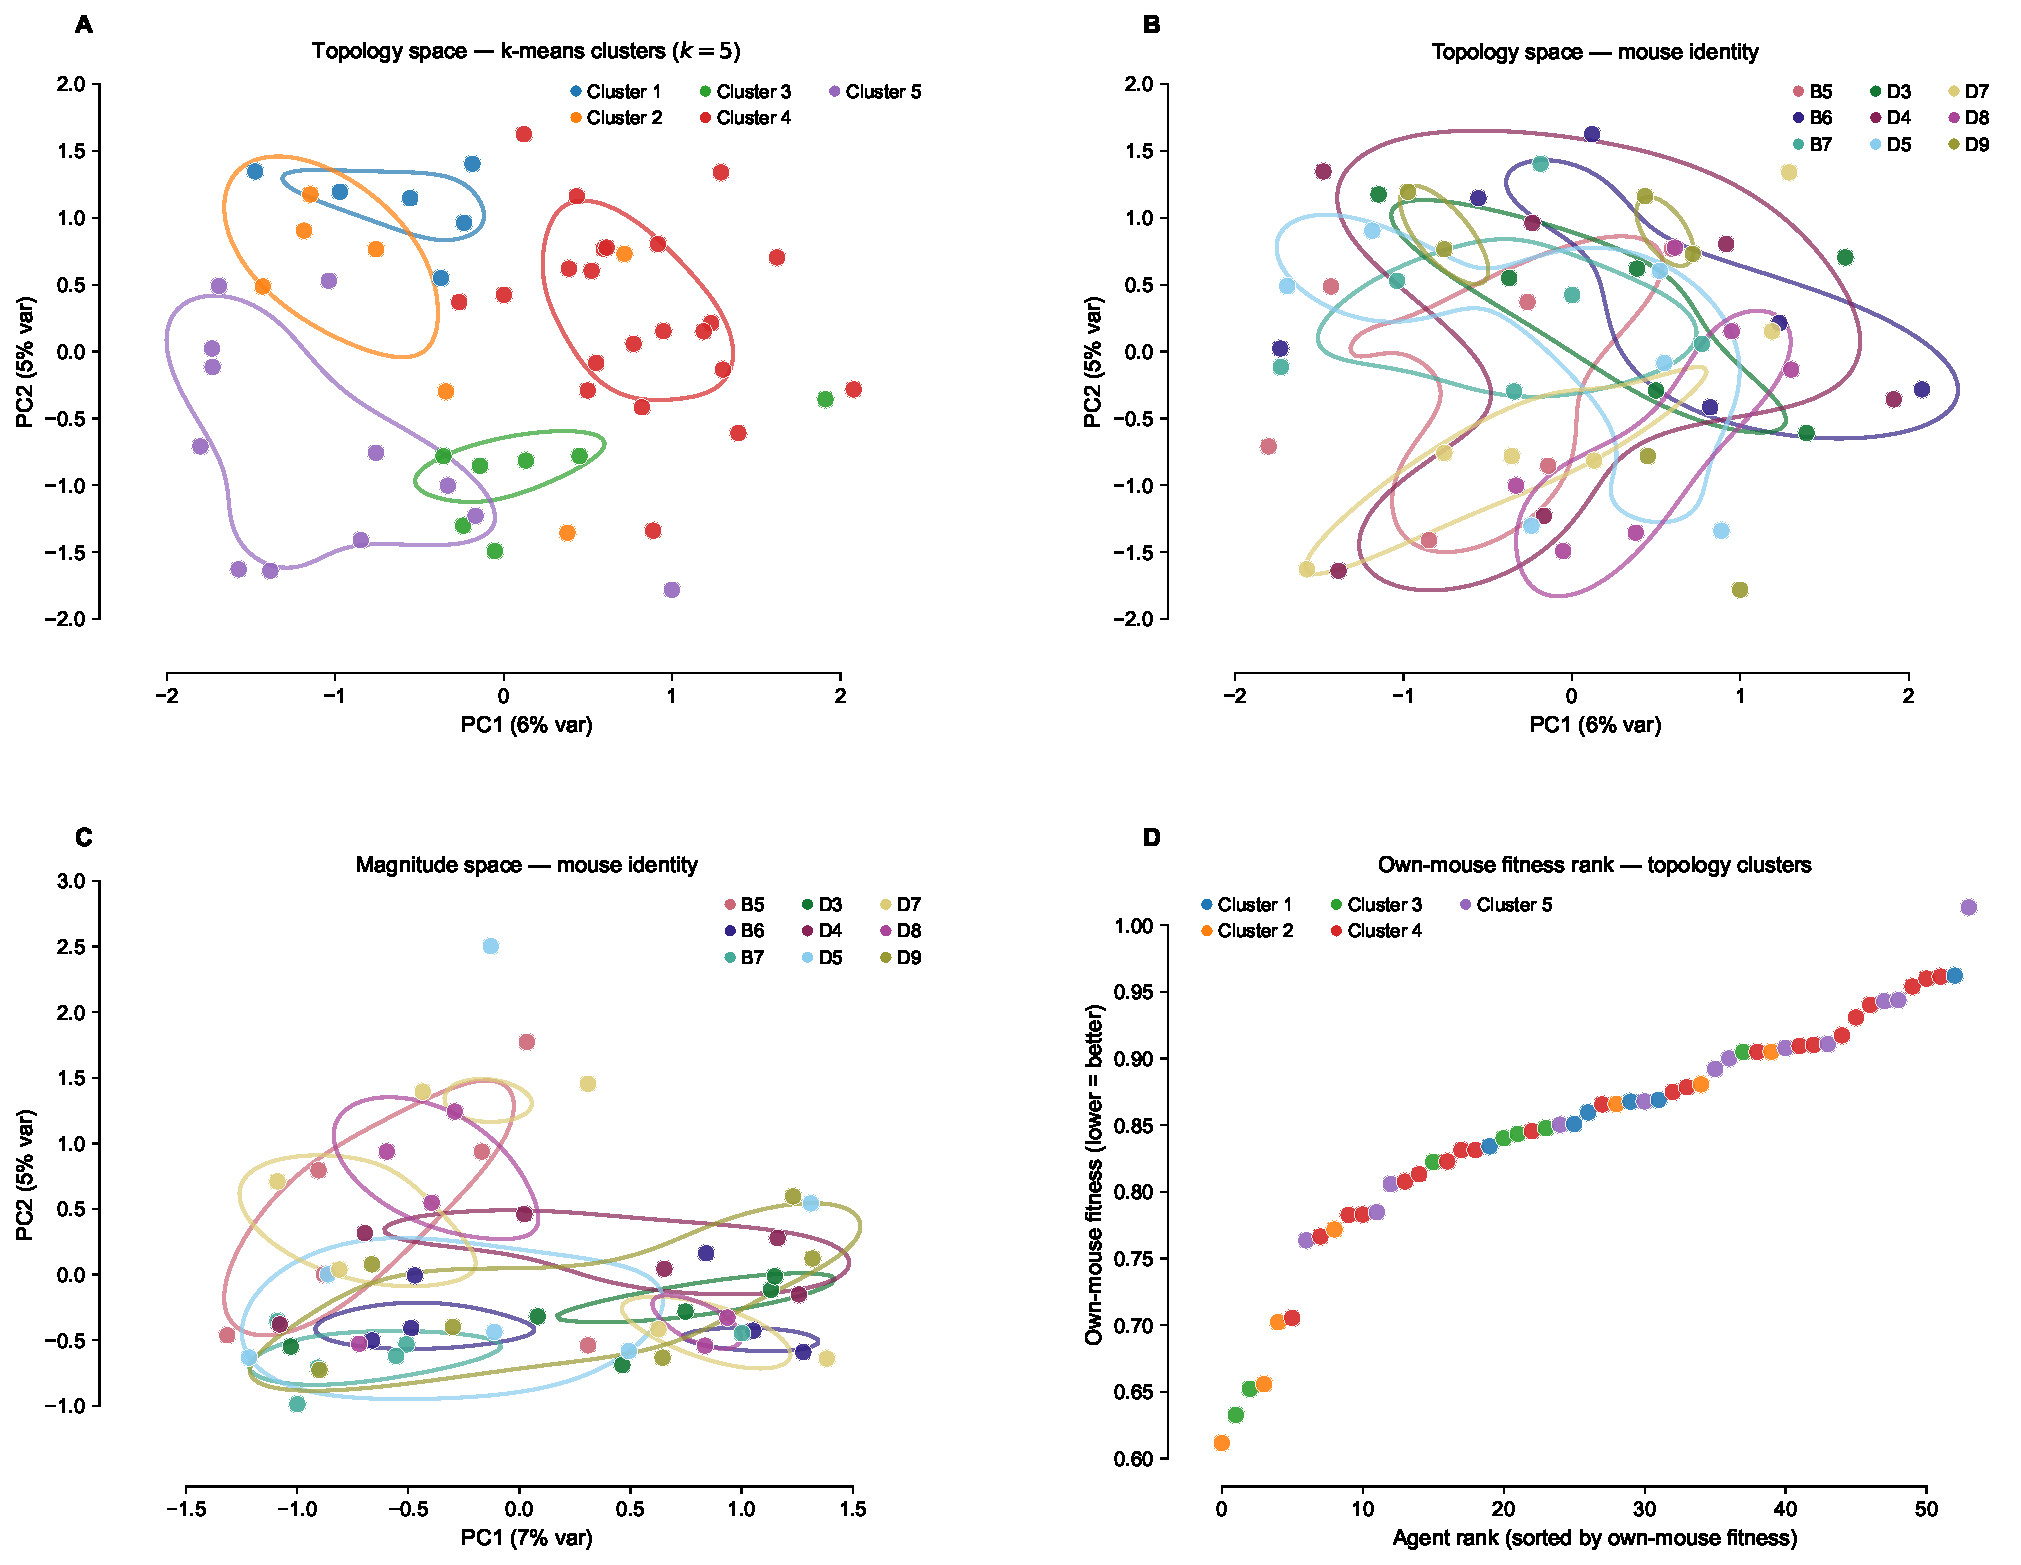
\includegraphics[width=\textwidth]{supp_mi_clustering.pdf}
  \caption{\textbf{Structural k-means clusters do not correspond to mouse identity or
  behavioral performance.}
  (A)~PCA of all 54 agents in topology feature space ($14 \times 14$ binary adjacency,
  196-dimensional), colored by k-means cluster assignment ($k = 5$, blue palette).
  Five structural groups are visible.
  (B)~Same topology PCA, colored by mouse identity (Tol palette, 9 mice). Agents from
  the same mouse are distributed across all structural clusters: topology is degenerate
  with respect to mouse identity.
  (C)~PCA of magnitude feature space, colored by mouse identity. The null replicates on
  a different structural axis.
  (D)~All 54 agents ranked by own-mouse fitness (lower = better; best on left), colored
  by topology cluster. Mixed colors across the performance rank confirm that structurally
  similar agents do not perform similarly: the fitness-quintile companion to the
  mouse-identity MI analysis in the main text.
  Percentage variance explained by PC1 and PC2 shown on axes A--C.}
  \label{fig:supp_mi_clustering}
\end{figure}

% ----------------------------------------------------------------------------

\subsection*{S14. Sensitivity RSA: the geometry of sensitivity profiles does not fingerprint mouse identity}
\label{sec:supp_sensitivity_rsa}

To test whether the full 14-dimensional sensitivity profile holistically
fingerprints mouse identity, we performed a representational similarity analysis
(RSA). We computed pairwise Euclidean distances between agents' 14-dimensional
ablation sensitivity vectors, yielding a $54 \times 54$ sensitivity RSM. We then
tested whether within-mouse pairs have lower sensitivity distance than between-mouse
pairs (Mann-Whitney $U$, $p = \statDegAfourMwP$) and whether the sensitivity RSM
correlates with a mouse-identity RSM (Mantel test: $\rho = \statDegAfourMantelRho$,
permutation $p = \statDegAfourMantelPPerm$; 10,000 permutations).

Both tests are null. The \emph{geometry} of the sensitivity profile does not
fingerprint mouse identity: agents trained on the same mouse are no more similar
in their sensitivity profiles than agents trained on different mice. This is
consistent with the per-source ablation null (0/14 neurons significant; reported
in Section~\ref{sec:causal}), and together they rule out any structural
decomposition of the sensitivity profile as a mouse-identity fingerprint. The
result that individuates specialists from generalists is not the \emph{pattern}
of sensitivity but its \emph{variance} (Section~\ref{sec:sensitivity}).

Note: this analysis is likely underpowered at $n = 6$ replicates per mouse.
Additional replicates are planned (see Section~\ref{sec:disc_limitations}).

\begin{figure}[H]
  \centering
  
\includegraphics[width=0.7\textwidth]{A4_sensitivity_RSA.png}
  \caption{\textbf{Sensitivity RSA: no mouse-level structure.}
  Left: $54 \times 54$ sensitivity RSM (pairwise Euclidean distance between
  ablation sensitivity vectors), agents ordered by mouse. No block-diagonal
  structure is visible. Right: within-mouse vs between-mouse sensitivity
  distance distributions (Mann-Whitney $p = \statDegAfourMwP$).}
  \label{fig:supp_sensitivity_rsa}
\end{figure}

% ----------------------------------------------------------------------------

\subsection*{S15. Representational geometry: positive control and robustness}
\label{sec:supp_rep_geometry}

\begin{figure}[H]
  \centering
  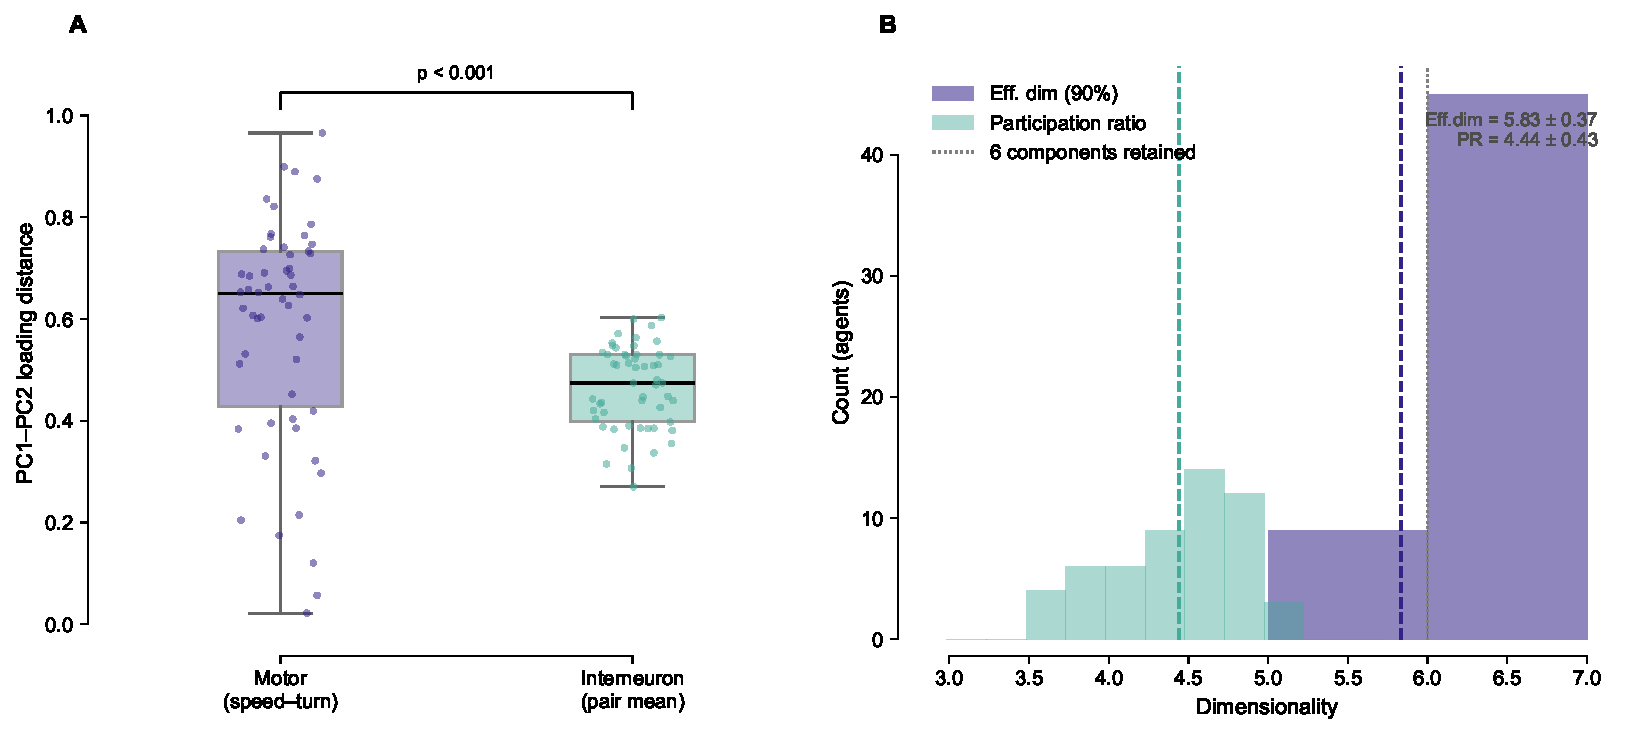
\includegraphics[width=\textwidth]{fig_supp_act_emb_ctrl.pdf}
  \caption{\textbf{Activity embedding positive control.}
  Motor neuron separation in PC1--PC2 loading space as a sanity check for
  embedding informativeness at the small scale of these networks ($N=14$).
  Speed (neuron~12) and Turn (neuron~13) motor neurons are consistently more
  separated from each other than the typical interneuron pair
  ($\statActEmbMotorDist \pm \statActEmbMotorDistStd$ vs
  $\statActEmbInterDist \pm \statActEmbInterDistStd$; Mann-Whitney $p < 0.001$),
  confirming that neuronal embeddings capture functional circuit structure despite
  the small network size.}
  \label{fig:supp_act_emb_ctrl}
\end{figure}

\begin{figure}[H]
  \centering
  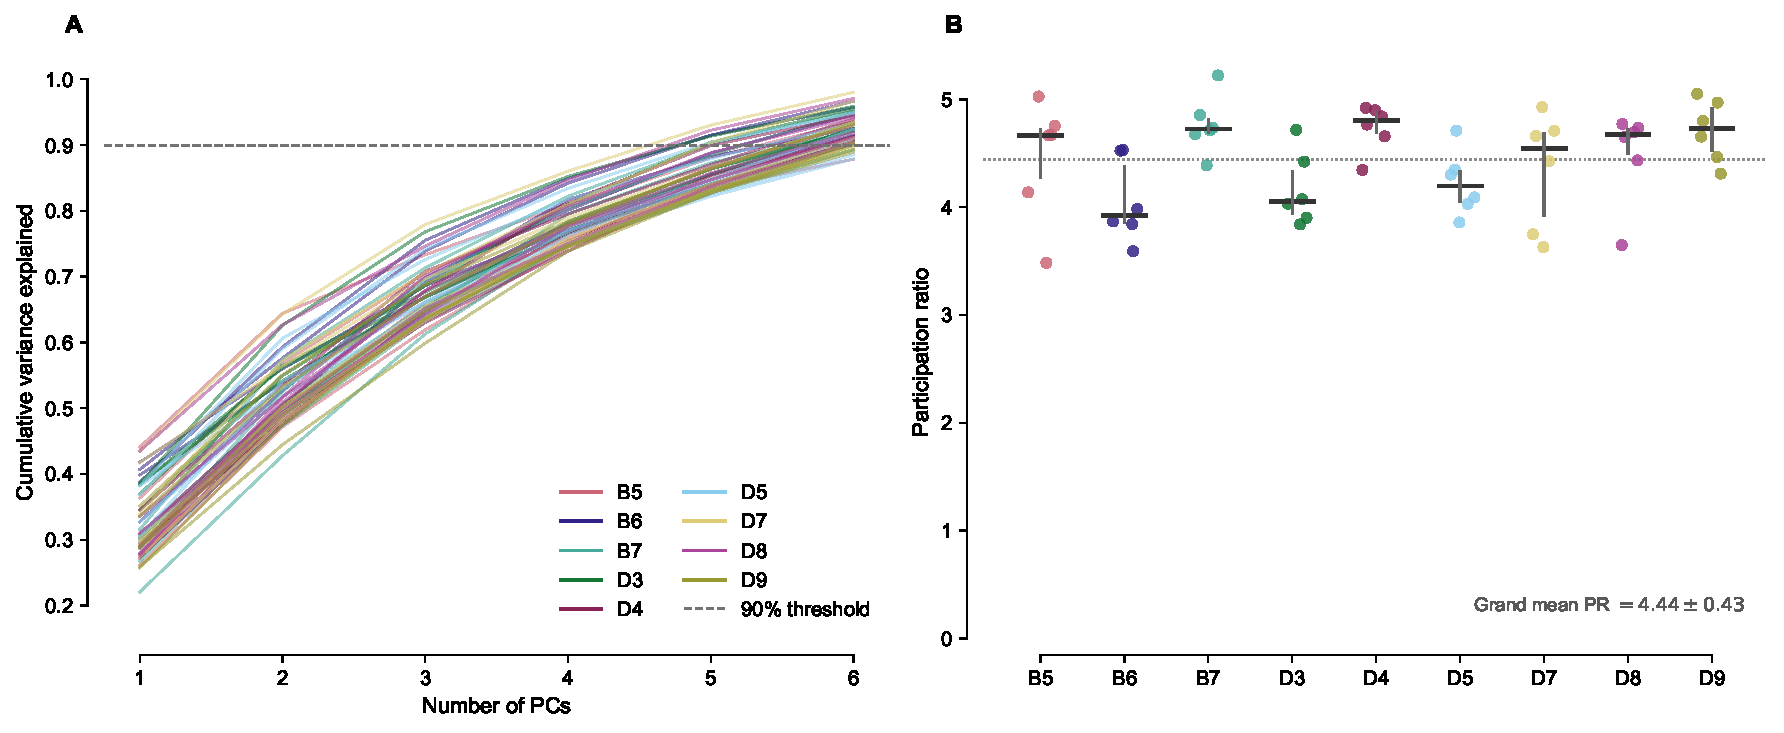
\includegraphics[width=\textwidth]{fig_supp_b3_dim.pdf}
  \caption{\textbf{Manifold dimensionality is near-maximal and uniform across mice.}
  \emph{Left:} Cumulative variance explained by the top 6 PCs for each of the 54 best-evolved
  agents (lines coloured by mouse). The 90\% threshold (dashed grey) is reached by PC~5--6
  in all agents, justifying retention of 6 components. Curves are highly consistent across
  mice, with no mouse-specific variance structure.
  \emph{Right:} Participation ratio (PR) per mouse (strip plot with median and IQR; one dot
  per agent). Grand mean PR $= \statActEmbPR \pm \statActEmbPRStd$ out of a maximum of 6,
  corresponding to effective dimensionality $\statActEmbEffDim \pm \statActEmbEffDimStd$.
  No mouse shows a distinctively lower or higher dimensionality, confirming that individual-target
  selection does not compress or expand the dimensionality of representational space.}
  \label{fig:supp_b3_dim}
\end{figure}

\begin{figure}[H]
  \centering
  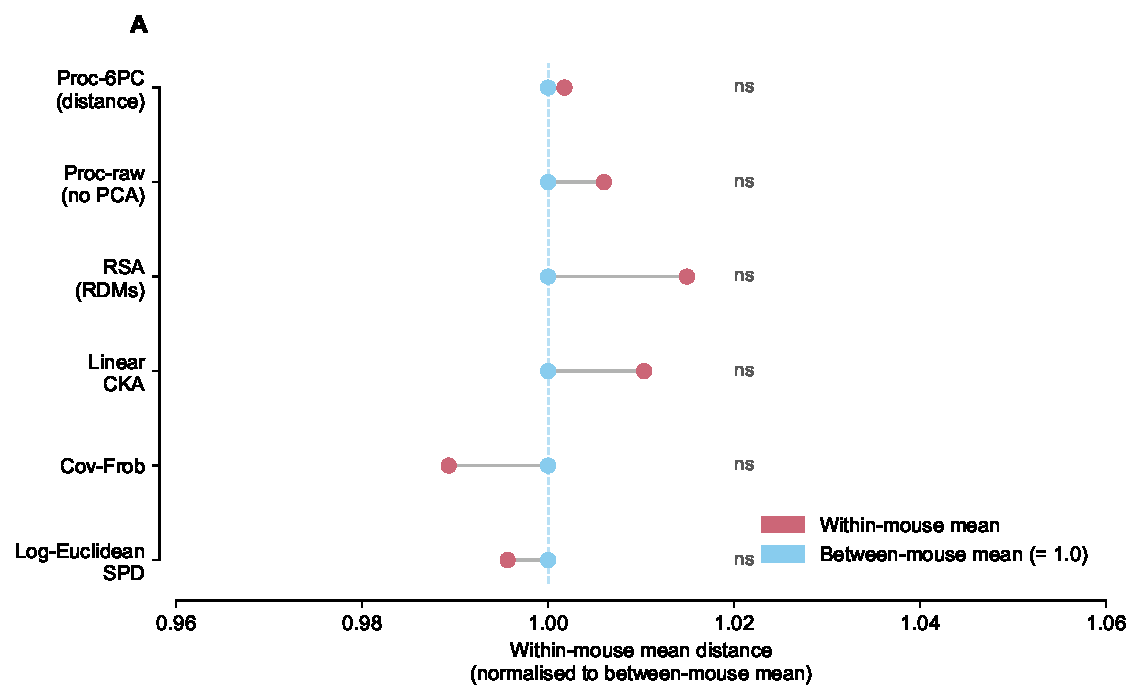
\includegraphics[width=0.72\textwidth]{fig_supp_emb_robustness.pdf}
  \caption{\textbf{Representational degeneracy is robust across six independent similarity metrics.}
  Within-mouse mean distance (red) versus between-mouse mean distance (blue, set to 1.0
  for each method) for six metrics applied to the same 54 agent activity records.
  Proc-6PC: Procrustes distance on 6-PC loading matrices (main analysis). Proc-raw: Procrustes on raw per-bout means without PCA. RSA: representational
  dissimilarity analysis on per-bout response RDMs. CKA: centred kernel alignment. Cov-Frob:
  Frobenius distance between neuron-neuron covariance matrices. Log-Euclidean SPD:
  affine-invariant distance on the SPD manifold. All pairwise comparisons are
  indistinguishable (all MW $p > 0.25$, ns), ruling out PCA truncation or a particular
  distance convention as an explanation for the null result.}
  \label{fig:supp_emb_robustness}
\end{figure}

% ----------------------------------------------------------------------------

\subsection*{S16. Dynamical null results}
\label{sec:supp_dynamics}

Trajectory RSM and Lyapunov analyses used a standardised synthetic sensory input
sequence (Section~\ref{sec:methods_specificity}). Activation trajectory cosine
similarities and Lyapunov exponents ($\lambda_1$) showed no between-mouse
differences (trajectory RSM: $p = \statDynamicsTrajectoryP$; Lyapunov:
$p = \statDynamicsLyaP$; fixed-point eigenvalue: $p = \statDynamicsLamP$).
Grand mean $\lambda_1 = \statDynamicsLyaMean \pm \statDynamicsLyaStd$, confirming
a uniform slightly stable dynamical regime across all mice.

\begin{figure}[H]
  \centering
  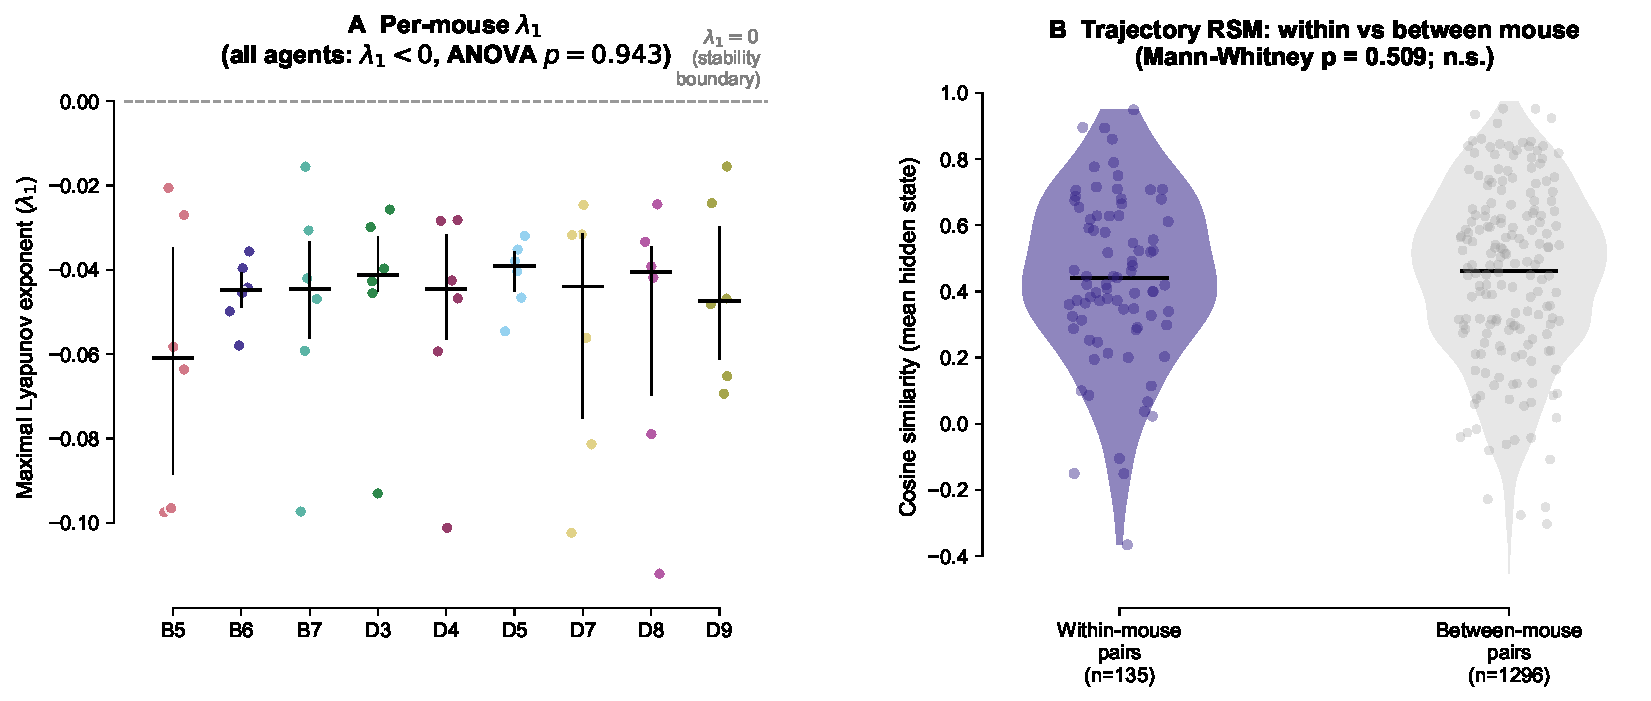
\includegraphics[width=\textwidth]{fig_s17_dynamics_null.pdf}
  \caption{\textbf{Dynamical null results.}
  (A)~Per-mouse maximal Lyapunov exponent $\lambda_1$ (strip plot; median and IQR shown).
  All 54 agents are slightly stable ($\lambda_1 < 0$); one-way ANOVA returns
  $F = \statDynamicsLyaF$, $p = \statDynamicsLyaP$ --- no mouse-specific stability
  signature.
  (B)~Within-mouse (purple) versus between-mouse (grey) activation trajectory cosine
  similarity (violin + strip). Distributions are indistinguishable
  (Mann-Whitney $p = \statDynamicsTrajectoryP$; n.s.).}
  \label{fig:supp_dynamics_null}
\end{figure}

% ----------------------------------------------------------------------------

\subsection*{S17. Attractor landscape analysis}
\label{sec:supp_attractor}

Each agent was run from 200 random initial states with zero sensory input for 500
steps to map its autonomous attractor landscape. Final interneuron and motor states
(8-dimensional) define an attractor fingerprint per agent. Pairwise sliced Wasserstein
distances between agent attractor distributions showed no within-mouse clustering
(within $\statActEmbAttrWithinWass \pm \statActEmbAttrWithinWassStd$ versus
between $\statActEmbAttrBetweenWass \pm \statActEmbAttrBetweenWassStd$;
Mann-Whitney $p = \statActEmbAttrMwP$).

\begin{figure}[H]
  \centering
  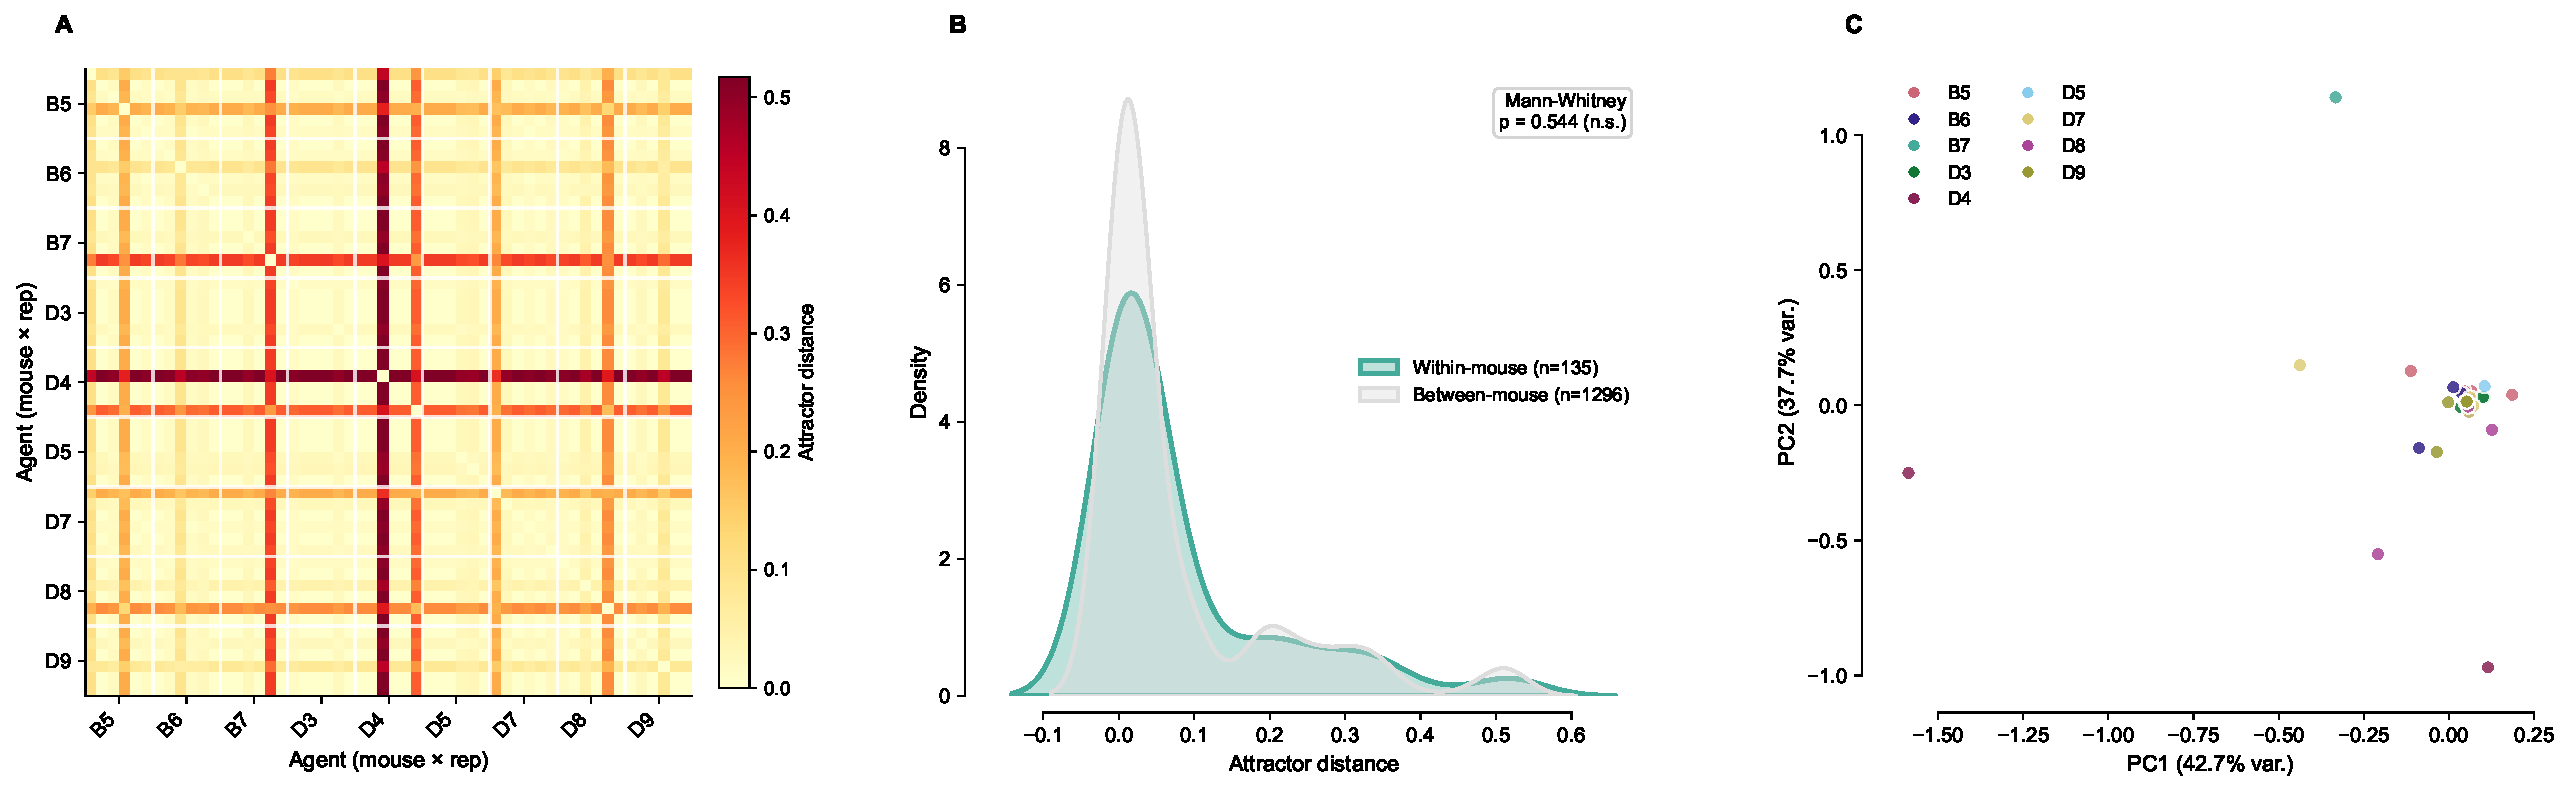
\includegraphics[width=\textwidth]{fig_supp_d4_attractor.pdf}
  \caption{\textbf{Attractor landscape is degenerate across mice.}
  \emph{Left:} $54 \times 54$ sliced Wasserstein distance matrix between agent attractor
  distributions (plasma scale). No block structure is visible.
  \emph{Centre:} KDE of within-mouse (red) versus between-mouse (blue) attractor
  distances (Mann-Whitney $p = \statActEmbAttrMwP$; n.s.).
  \emph{Right:} Attractor fingerprints in 2D (PCA of zero-input final states; one
  representative agent per mouse, 200 initial conditions each). Points coloured by mouse.
  No mouse-specific clustering is apparent.}
  \label{fig:supp_d4}
\end{figure}

% ---------------------------------------------------------------------------
\label{sec:supp_spec_evol_per_mouse}

Per-mouse specialisation trajectories. Figure~\ref{fig:supp_spec_evol_per_mouse}
shows the specialisation index (mean $\pm$ SD across 6 replicates) for each of the
9 mice independently over 150 generations. All mice develop positive specialisation
indices; the rate of emergence and final magnitude vary across mice, consistent with
the between-mouse variance visible in Figure~\ref{fig:paradox}E.

\begin{figure}[H]
  \centering
  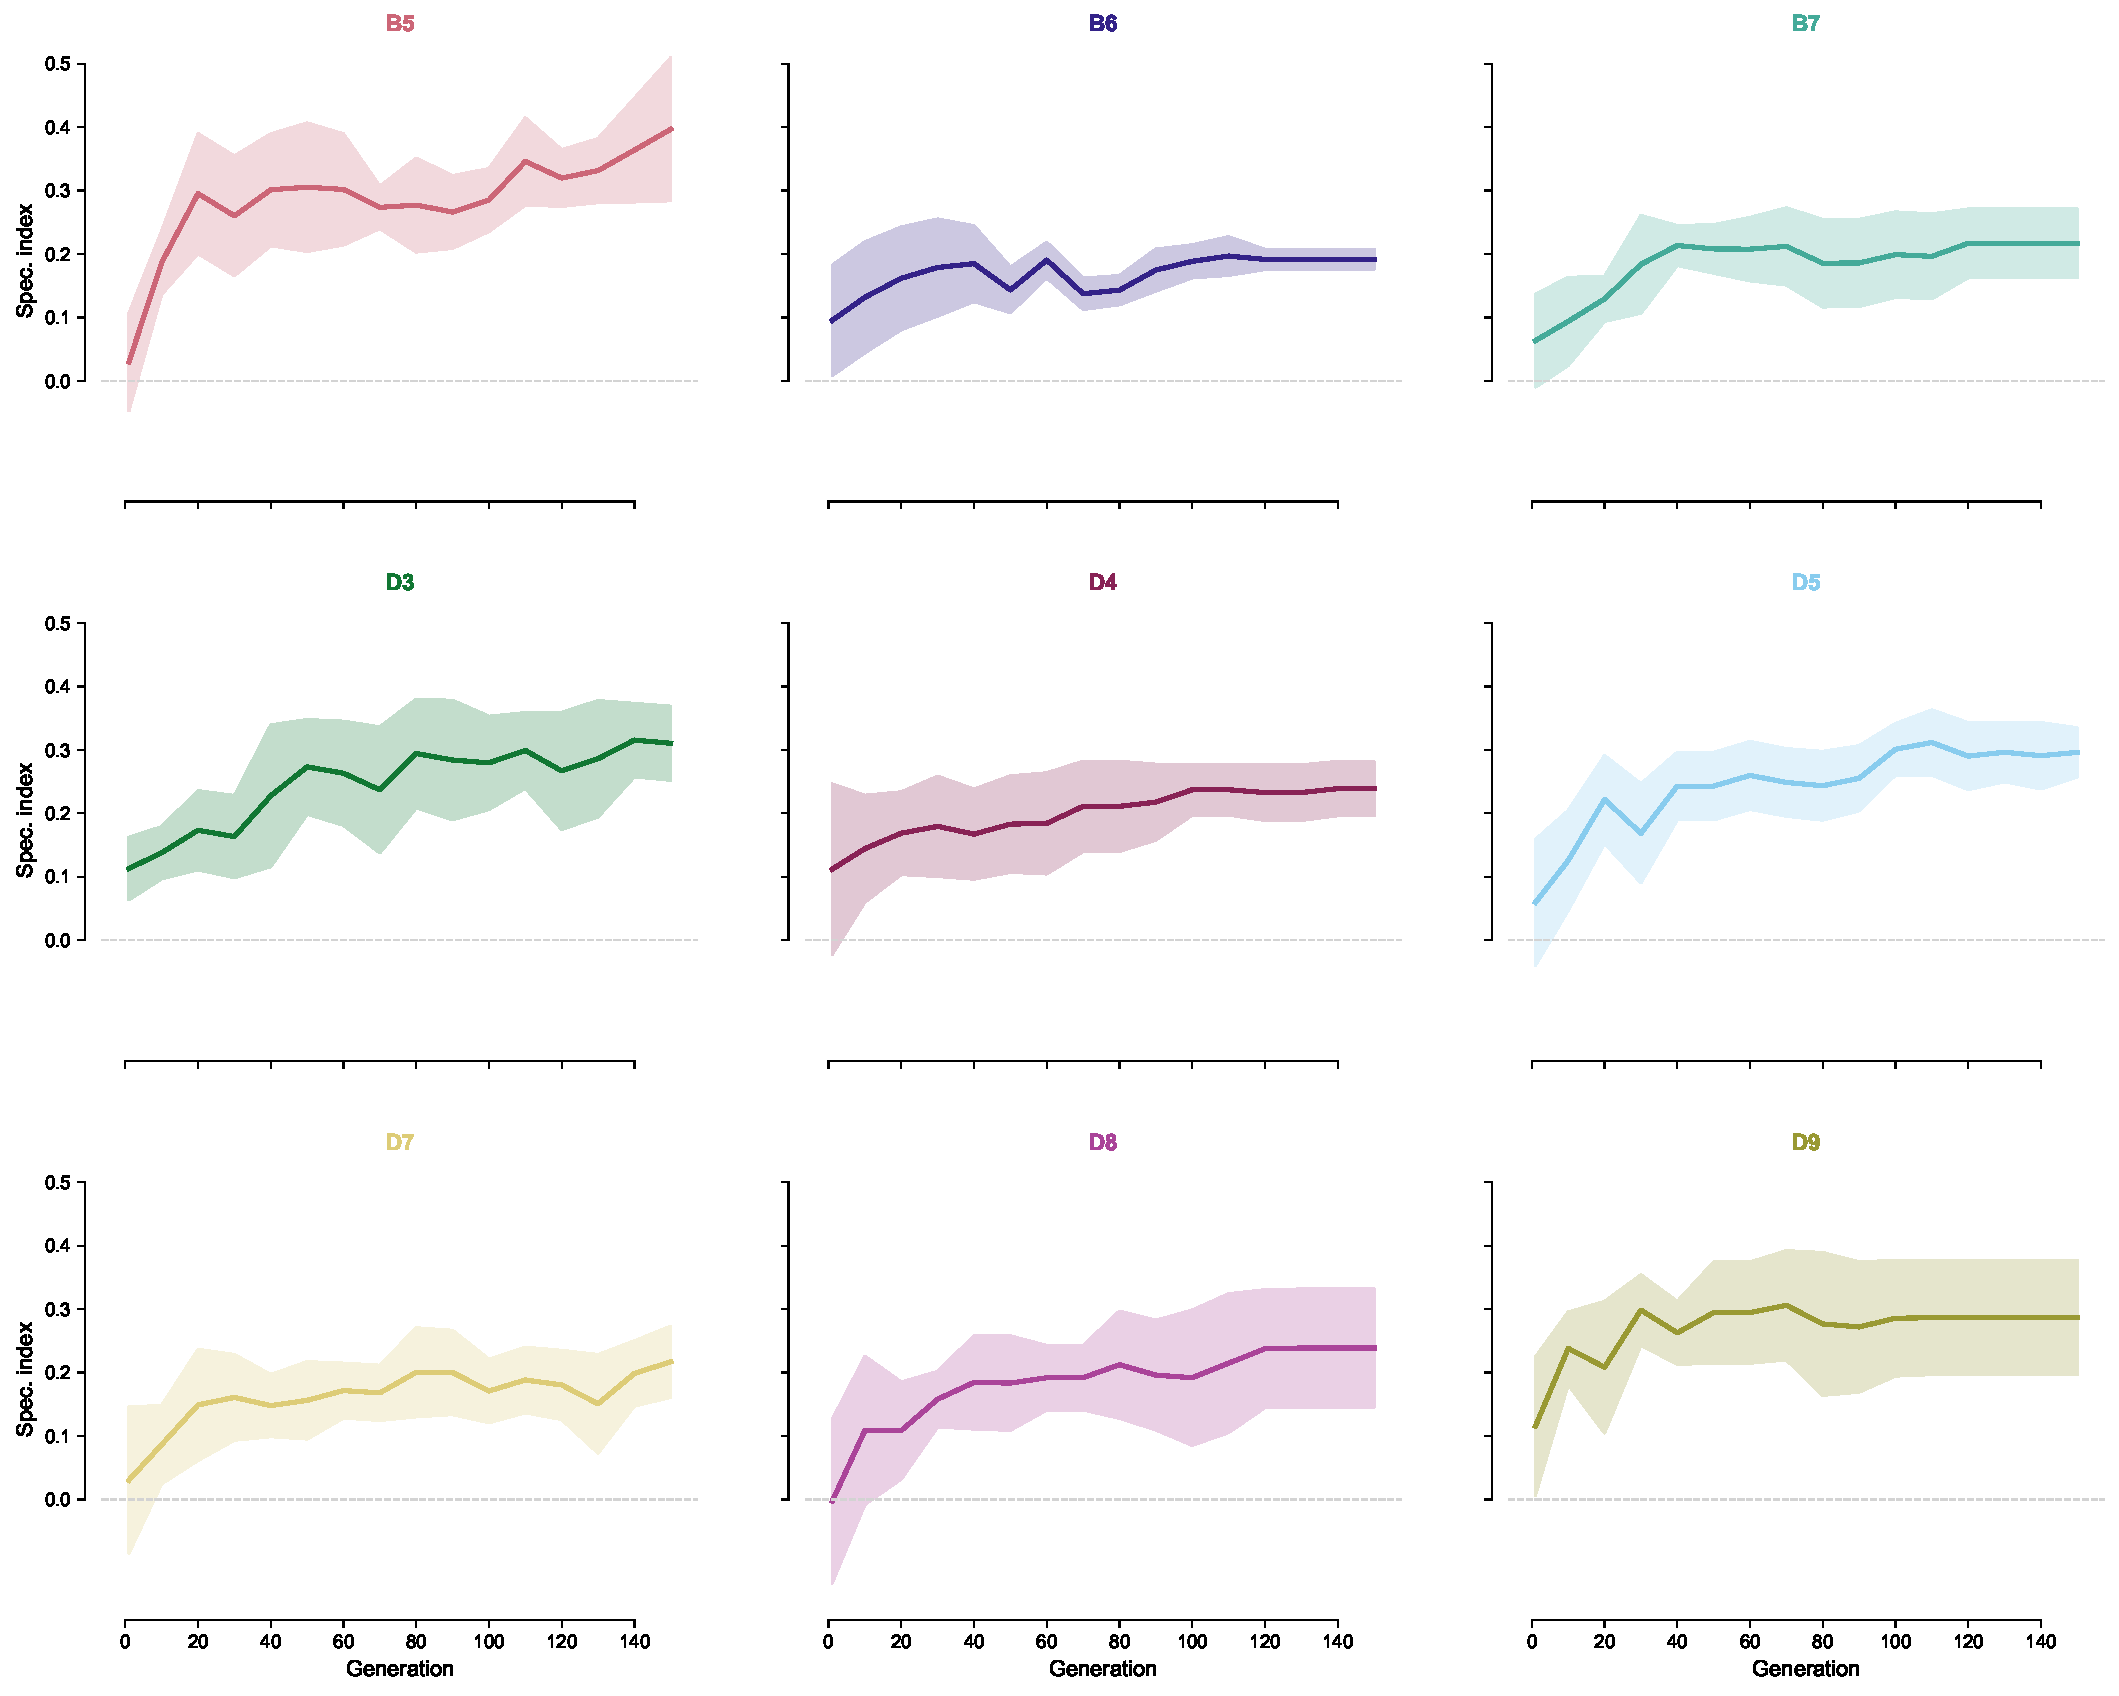
\includegraphics[width=\textwidth]{fig_supp_spec_evol_per_mouse.pdf}
  \caption{\textbf{Per-mouse specialisation index trajectories.}
  Specialisation index (mean $\pm$ SD, $n = 6$ replicates) over 150 generations for
  each of the 9 mice. Each panel corresponds to one mouse (colour-coded as in main
  figures). All mice reach positive specialisation indices; variance across replicates
  narrows with increasing generations.}
  \label{fig:supp_spec_evol_per_mouse}
\end{figure}

% ---------------------------------------------------------------------------
\label{sec:supp_sens_commitment_evo}

Sensitivity commitment co-develops with behavioural specialisation.
Figure~\ref{fig:supp_sens_commitment_evo} shows three temporal analyses from
the same generation checkpoints used in the main specialisation trajectory.
Panel~A reproduces the population mean specialisation index for reference.
Panel~B shows mean per-neuron sensitivity variance over generations for
specialists (blue) and generalists (orange) on a log scale; specialist variance
remains elevated relative to the generalist level from approximately generation~20
onward, indicating that the higher sensitivity commitment seen at generation~150
builds progressively rather than emerging late.
Panel~C shows pairwise cosine similarity of sensitivity profile vectors: within
the same mouse (solid) vs between mice (dashed). Within-mouse cosine similarity
falls below the between-mouse baseline over training, indicating that replicates
targeting the same mouse develop idiosyncratic mouse-specific sensitivity
profiles rather than converging on a single canonical solution~---~a further
expression of functional degeneracy within the commitment regime.

\begin{figure}[H]
  \centering
  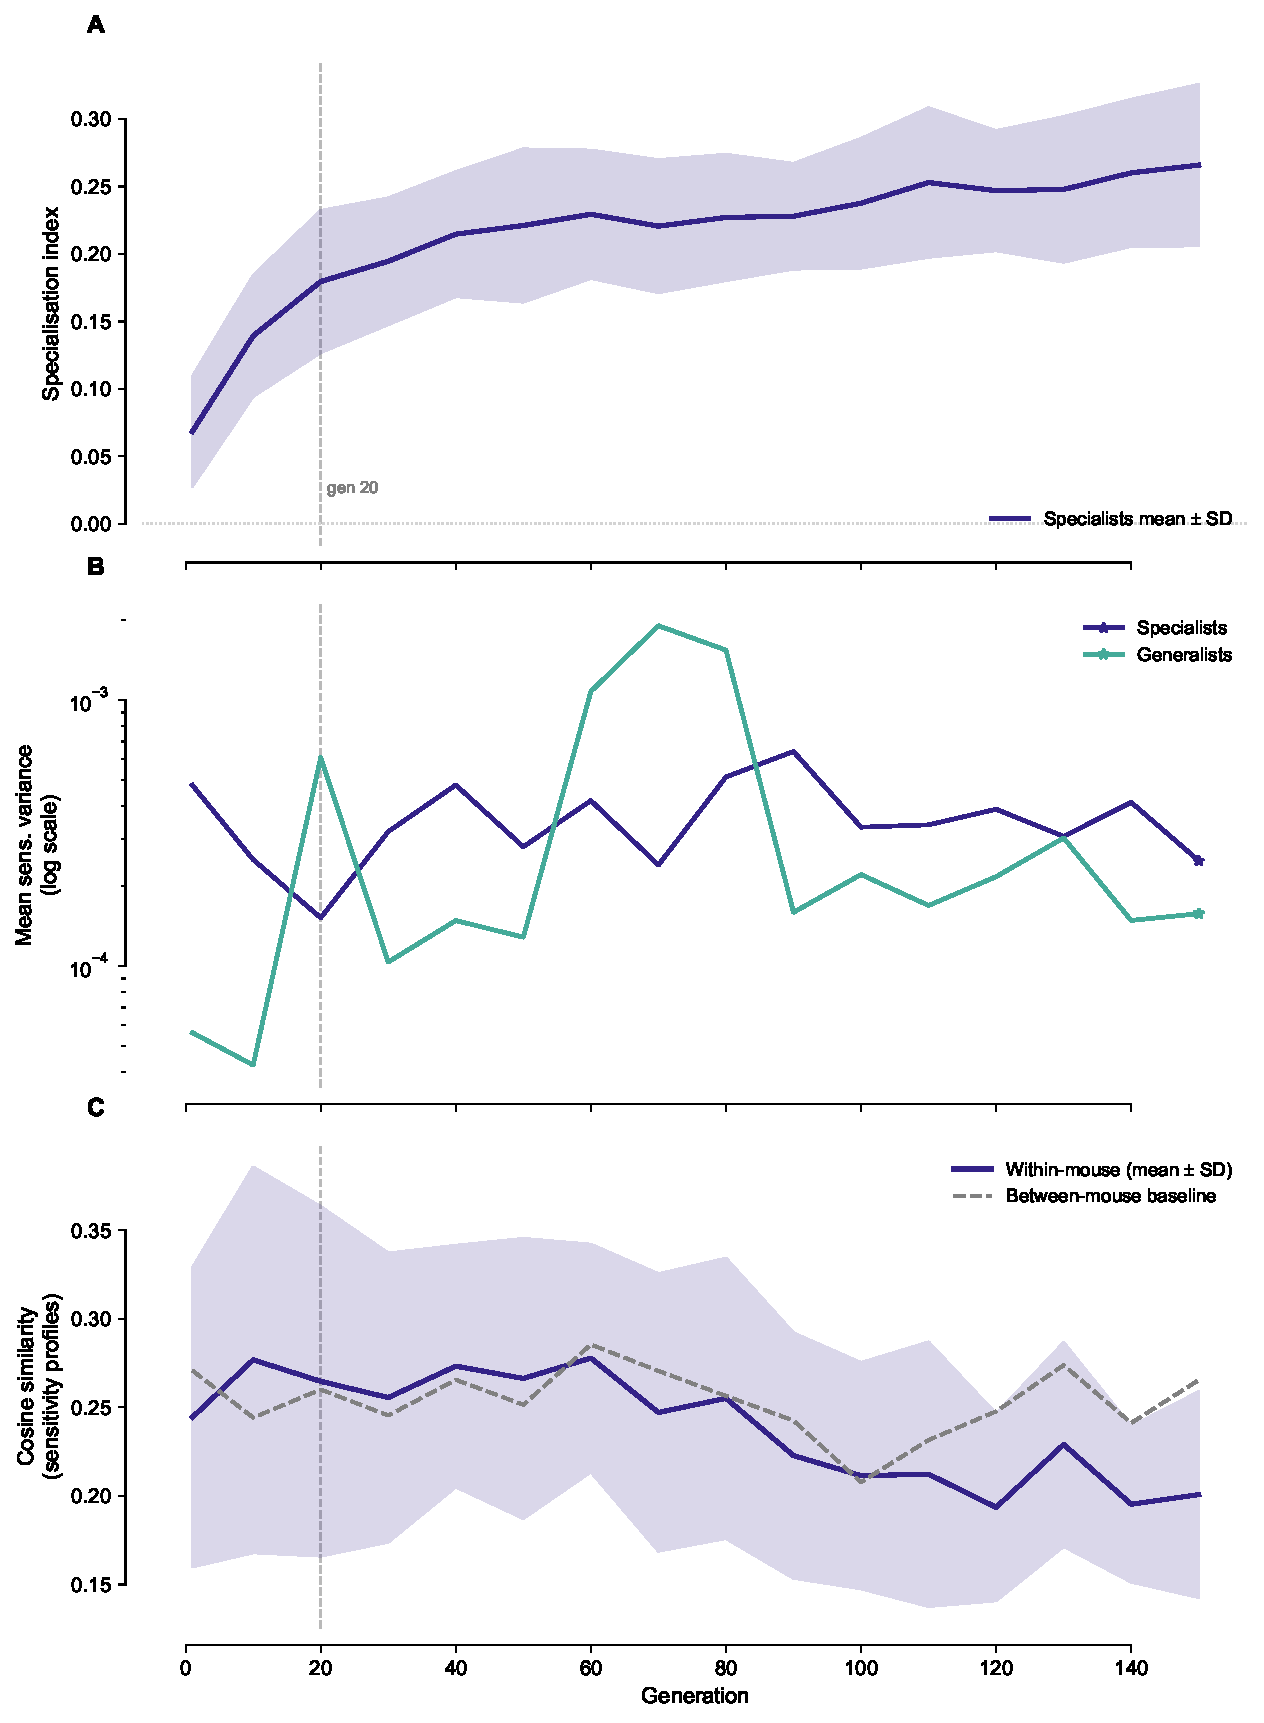
\includegraphics[width=0.75\textwidth]{fig_supp_sens_commitment_evo.pdf}
  \caption{\textbf{Sensitivity commitment temporal co-development.}
  (A)~Population mean behavioural specialisation index $\pm$ SD.
  (B)~Mean per-neuron sensitivity variance over generations: specialists (blue) vs
  generalists (orange), log scale. Dashed vertical line marks generation~20.
  (C)~Within-mouse pairwise cosine similarity of sensitivity profiles (solid line,
  $\pm$ SD shading) vs between-mouse baseline (dashed). Within-mouse similarity
  falls below the between-mouse baseline from approximately generation~50, indicating
  divergence of idiosyncratic mouse-specific sensitivity patterns across replicates.}
  \label{fig:supp_sens_commitment_evo}
\end{figure}

\end{document}

